% started at Sun Dec 20 18:29:58 CST 2015
% written by wuzhouhui250@gmail.com
% compiled by xelatex
% vim: ts=4 sts=4 sw=4 et tw=75

% vim: ts=4 sts=4 sw=4 et tw=75
% preamble here.

\documentclass[nofonts, oneside]{ctexbook}

\usepackage{geometry}
\usepackage{fontspec}
\usepackage{xeCJK}
\usepackage{amssymb}
\usepackage{hyperref}
% for number of footnote
\usepackage{pifont}
% 一页结束时, 脚注编号清零
\usepackage[perpage]{footmisc}
% verbatim and endverbatim
\usepackage{graphicx}
\usepackage{listings}
\usepackage{multicol}
\usepackage{tocloft}
\usepackage{graphics,graphicx,pdfpages}

% for fixing "Unable to load picture or PDF file 'bc-book.mps'"
\DeclareGraphicsRule{.mps}{eps}{*}{}

% 脚注编号带圈
\renewcommand\thefootnote{\ding{\numexpr171+\value{footnote}}}

% from package geometry
% 为边注加边框
\let\oldmarginpar=\marginpar
\renewcommand\marginpar[1]{%
    \oldmarginpar{\framebox{#1}}%
}
\geometry{%
	margin=1cm,
	marginparsep = 0.5cm,
	marginparwidth=1cm,
	top = 3cm,
	bottom = 3cm,
	outer = 3cm,
	inner = 3cm
}

% from package hyperref
\hypersetup{
    bookmarksnumbered = true,
    pdftitle = {Hacking Vim 7.2},
    pdfcreator = {https://m-mono.github.io},
    pdfauthor = {Kim Schulz},
    pdfsubject = {深入 Vim 7.2},
    colorlinks = false,
    pdfborder = 0 0 0,
    pdfkeywords = {不知道是谁 说过一句话:说世界上的程序员分为三种,一种是使用Vim的,还有一种使用Emacs的,剩下的都是第三种。由此可见Vim的强大程度,可以说,这是一款非常适合程序员使用的编辑器。Vim的设计哲学是如果你的工作只需要做一次,那没问题,怎么搞都行,如果你的工作是要重复的完成某些工作,则Vim总可以帮你找到更少的按键方式来实现相同的目标,为此,Vim设计了多种模式,常见的模式包括命令模式,编辑模式,命令模式等,这个也是和其他编辑器一个很不相同的地方,可能有些已经有其他编辑器习惯的人有点不太习惯的地方,但是如果将模式熟悉了就可以发现在不同的模式之间切换是很平常的事情,而且带来的好处是更少的按键和更快的输入。}
}




%\setCJKfamilyfont{heiti}{FandolHei}
% 章节格式
%%\CTEXsetup[format={\CJKfamily{heiti}\large\upshape}]{subsection}
%%\CTEXsetup[numberformat={\CJKfamily{heiti}\large\upshape\bfseries}]{subsection}
%%\CTEXsetup[format={\CJKfamily{heiti}}]{subsubsection}
% 目录格式
%\renewcommand\cftchapfont{\CJKfamily{heiti}}
\settowidth\cftchapnumwidth{第几十几章} % 最宽的可能编号
\renewcommand\cftchapaftersnumb{\hspace{2.2em}} % 额外间距

% from package fontspec and xeCJK
\setCJKmainfont[Path=Fonts/]{Inziu-Iosevka-SC-Regular.ttf}
\setCJKsansfont[Path=Fonts/]{Inziu-Iosevka-SC-Regular.ttf}
\setCJKmonofont[Scale=0.9,Path=Fonts/]{Inziu-Iosevka-SC-Regular.ttf}
\setmainfont[Path=Fonts/]{Inziu-Iosevka-SC-Regular.ttf}
\setsansfont[Path=Fonts/]{Inziu-Iosevka-SC-Regular.ttf}
% "Mapping={}" make quote symbol straight
\setmonofont[Mapping={},Path=Fonts/]{SourceCodePro-ExtraLight.ttf}

\newcommand\vi{\texttt{vi}}
\newcommand\vim{\texttt{vim}}

% TODO: warning 与 tips 环境有一对中括号, 而且高度随内容而改变.
\newenvironment{warning}%
{
    \begin{quotation}
        \parbox[c]{4em}{\includegraphics[scale=1.8]{./images/bc-book.mps}}
    \begin{minipage}{33em}
}
{
    \end{minipage}
    \end{quotation}
}

\newenvironment{tips}%
{
    \begin{quotation}
        \parbox[c]{4em}{\includegraphics[scale=1.8]{./images/bc-lampe.mps}}
    \begin{minipage}{33em}
}
{
    \end{minipage}
    \end{quotation}
}

\newcommand\file[1]{\texttt{#1}}
\newcommand\newterm[1]{#1}
\newcommand\email[1]{\href{mailto:#1}{#1}}
\newcommand\key[1]{\textit{#1}}

\newenvironment{vimcmdform}
    {\list{}{\leftmargin=2em\rightmargin=0em}\item[]}
    {\endlist}

\lstnewenvironment{vimcode}
    {\lstset{basicstyle=\ttfamily,
        xleftmargin=2em,
        breaklines=true,
        tabsize=4}}
    {}

\title{Hacking Vim 7.2 / 深入 Vim 7.2}
\author{Kim Schulz}
\begin{document}
	\begin{figure}[ht]
		\begin{center}
			
\includepdf[width=\paperwidth]{Title.jpg}
		\end{center}
	\end{figure}
	\newpage
	
\frontmatter
\pdfbookmark[0]{封面}{title}
\maketitle
\pdfbookmark[0]{目录}{contents}
\tableofcontents
% vim: ts=4 sts=4 sw=4 et tw=75
\chapter{前言}
\label{chap:preface}
\marginpar{1}
在计算机发展的早期,系统资源非常有限,开发人员必须想尽办法优化他们的应用程序,文本编辑器也是如此。Vim是当时最流行的编辑器之一,因为系统资源方面的限制,它被优化得近乎完美。\\

从那以后,计算机技术得到了快速的发展,虽然系统资源已经没有以前那么紧张了,但是Vim仍然坚持最初的原则。\\

乍看起来,Vim好像并没有什么值得称道的地方,但是,如果你能透过它简单的用户界面看到其本质,就会明白为什么到了如今这个年代,Vim仍然是众多用户最喜爱的编辑器。\\

它几乎囊括了你想要的任何一个功能,即使有所遗漏,也可以通过插件或脚本来实现。正是由于其出色的灵活性,使得它成为了众多任务的理想工具,以及世界上最先进的编辑器之一。\\

每天都有大量的新用户加入Vim社区,并开始用Vim处理他们的日常工作.虽然有时候使用起来比较复杂,但是与其他编辑器相比,人们还是更愿意选择Vim,本书就是为这些用户而写。\\

通过阅读本书,用户可以更加得心应手地使用Vim,从而提高工作效率。他们得到的不仅仅是一个优化的编辑器,还有优化的工作流程。本书帮助用户更加自如地使用Vim,从把它当作一个简单的文本编辑器开始,一直到其他日常工作,Vim都可以胜任。\\

祝你阅读愉快!

\section*{本书主要讨论什么}
\marginpar{2}
第\ref{chap:getting_started_with_vim}章: 开始,介绍Vim和它的几个比较有名的亲戚,并简要介绍它们和 vi 的关系及其历史。\\

第\ref{chap:personalizing_vim}章: 定制Vim,介绍如何配置Vim,使得它更符合用户的个人需求。主要介绍如何修改字体,配色方案,状态行,菜单,与工具条。\\

第\ref{chap:better_navigation}章: 快速导航,介绍一些在多个文件中快速导航的方法,通过这些方法,读者可以轻松地在多个文件之间穿梭。\\

第\ref{chap:production_boosters}章: 助推器,介绍Vim的若干特性,描述了模版,自动补全,拆叠,会话,和寄存器的使用方法。\\

第\ref{chap:advanced_formatting}章: 格式化进阶,讨论如何对文本和代码进行格式化。它还介绍了如何借助外部工具,使得Vim更加完美。\\

第\ref{chap:basic_vim_scripting}章:Vim脚本基础,这一章是为那些想通过脚本来扩展Vim功能的人而准备的,它介绍了脚本的基础知识,经过这一章的学习,读者应该能够写出一些简单的脚本。\\

第\ref{chap:extended_vim_scripting}:Vim脚本进阶,在第\ref{chap:basic_vim_scripting}章的基础上,再继续讲一些高级的脚本知识,包括如何在Vim脚本中使用外部的脚本语言。\\

附录 \ref{chap:vim_can_do_everything}: 无所不能的Vim,提供了一张游戏列表,它们都是用Vim脚本开发的,这一章还简单讨论了如何使用脚本实现聊天和邮件工具,另外还介绍了如何将Vim作为一个IDE使用。\\

附录 \ref{chap:vim_configuration_alternatives}:Vim配置管理,展示如何通过在线副本来更好地管理和获取Vim配置文件。\\

\section*{为了阅读本书,你还需要什么}
最近十年,Vim已经发展成一个功能非常丰富的编辑器,这同时意味着最新版的某些功能,旧版可能并不支持。\\

Vim 已经移植到了多种平台中,但并不是所有的功能对任意一种平台来说都是可用的。这主要是因为有些功能使用了和操作系统密切相关的特性,而这些特性在其他平台中可能并不提供。\\

\marginpar{3}
本书只关注Vim使用最广泛的两种平台:Linux与Microsoft Windows。由于Linux符合Unix标准,所以同样的结论在其他类Unix系统中仍然成立。\\

\begin{warning}
读者可以在 \url{www.vim.org} 上找到最新版的Vim源代码与二进制包。如果读者使用的是Linux,那么系统中很可能已经安装了Vim,而且是默认的编辑器。\\
\end{warning}

\section*{本书的目标读者}
\label{sec:who_this_book_is_for}
如果读者已经是一位Vim用户,而且想要学习更高级的技巧,那么这本书就是为你而写的。本书致力于帮助读者从一位Vim中级用户,上升为高级用户。\\

\section*{Vim 新手?}
\label{sec:new_to_vim}
虽然本书假设读者已经具备了Vim的基本知识,但即使是新手,本书也有一定的参考价值。\\

如果读者担心自己所掌握的Vim 知识不足以阅读此书,那么我建议你可以先看一下Vimtutor,在安装Vim时,会顺带安装这个Vim入门教程。\\

运行Vimtutor,然后跟着它学习Vim的基本使用方法,这大概需要30分钟。\\

Vimtutor支持多国语言,在启动程序时,可以通过指定国家代码来选择一种语言,国家代码由2个字母组成,比如ca,cs,de,el,eo,es,fr,hr,hu,it,ja,no,ro,和zh。例如,如果想要阅读德语版的Vimtutor,只需要在命令行执行\texttt{vimtutor de}。\\

\section*{排版约定}
\label{sec:conventions}
本书用不同风格的文本来表示不同种类的信息,这里有一些例子。\\

\marginpar{4}
包含在正文中的代码会这样显示:``键入 \texttt{:help 'statusline'},就可以打开Vim帮助系统,查看与状态行有关的全部帮助信息。''\\

代码块则是:
\begin{vimcode}
function! InfoGuiTooltip()
    "get window count
    let wincount = tabpagewinnr(tabpagenr(),'$')
    let bufferlist=''
    "get name of active buffers in windows
    for i in tabpagebuflist()
        let bufferlist .= '['.fnamemodify(bufname(i),':t').'] '
    endfor
    return bufname($).' windows: '.wincount.' ' .bufferlist ' '
endfunction
\end{vimcode}

命令模式的输入或输出写成:\\
\begin{vimcode}
:amenu icon=/path/to/icon/myicon.png ToolBar.Bufferlist :buffers<cr>
\end{vimcode}

\textbf{新的术语} \footnote{在中文版中并没有这样做 --- 译者注} 或\textbf{重点内容}加粗显示。读者在屏幕上看到的内容,比如菜单或对话框中的信息,会显示成:``这个命令在所有行的开头查找单词Error (用脱字符 \textasciicircum 标记)''。\\

\begin{warning}
这种文本框用来显示警告或重要的提示。\\
\end{warning}

\begin{tips}
这种文本框用来显示技巧和决窍。\\
\end{tips}

\section*{读者反馈}
\label{sec:reader_feedback}
对于读者的反馈我们总是非常欢迎。请把你关于这本书的想法告诉我们---不管是优点还是缺点,读者的反馈永远是我们不断进步的源泉。\\

反馈信息请发送到 \email{feedback@packtpub.com},并在邮件的主题中写上相关的书名。\\

\marginpar{5}
如果读者想向我们推荐书籍,请登陆\url{www.packtpub.com},在表单\texttt{SUGGEST A TITLE} 中填写相关的信息,或者发送邮件到\email{suggest@packtpub.com}。\\

如果你对某个主题很有研究,并且对写作也很感兴趣,请阅读\url{www.packtpub.com/authors} 的相关内容。\\

\section*{客户支持}
\label{sec:customer_support}既然读者买了 Packt 出版的书籍,那么我们会尽最大的努力让你觉得物有所值。\\
\begin{warning}
    下载书中的示例源代码:\\

    登陆 \url{http://www.packtpub.com/files/code/0509_Code.zip},下载书中的示例源代码,下载的文件中含有使用方法。\\
\end{warning}

\section*{勘误}
\label{sec:errata}

我们已经尽了最大的努力来保证内容的正确性,如果读者在书中发现了错误 --- 这个错误可能出现在正文中,也可能出现在代码中 --- 请把错误反馈给我们。通过反馈错误,可以帮助其他读者更顺利地阅读,也可以帮助我们提升后续版本的质量。无论读者发现了什么类型的错误,请登陆到\url{http://www.packtpub.com/support},选择对应的书籍,点击 \texttt{let us
know},然后输入相关的勘误信息。一旦勘误通过了校验,你的提交信息就会被接受,勘误也会上传到网页中,或者加到书籍勘误列表,这个列表可以在书籍的\texttt{Errata}部分找到。登陆\url{http://www.packtpub.com/support},选择对应的书籍,读者就可以找到该书所有的已知勘误。\\

\section*{版权声明}
\label{sec:piracy}

因特网物品的版权一直是一个让人头疼的问题。Packt 对版权和授权的保护向来非常重视,态度也很坚决。如果读者怀疑有人在因特网上非法复制我们的作品 --- 无论是什么形式 --- 请把相关的网址或网站名称发给我们(\email{copyright@packtpub.com}),这样我们才能快速地追回损失。希望读者能和我们一起尊重作者的辛勤付出,这样我们才能继续为你奉献精彩的作品。\\
\marginpar{6}

\section*{答疑}
\label{sec:questions}
无论你对书籍有什么疑问,都可以联系我们:\email{questions@packtpub.com},我们会尽最大的努力来回答你的问题。\\

\mainmatter
% vim: ts=4 sts=4 sw=4 et tw=75
\chapter{开始}
\label{chap:getting_started_with_vim}

\marginpar{7}
\newterm{Vim} (\newterm{Vi IMproved}) 编辑器最早由 Bram Moolenaar 于
1991 年 11 月发布, 当时只是作为 Unix vi 编辑器的 Amiga 平台克隆版.

一年后, Unix 平台的 Vim 发布, 接着, 它迅速成为了 vi 的替代版本.

由于宽松的授权和丰富的功能, 在开源社区的帮助下, Vim 逐渐流行起来.
越来越多的 Linux 发行版开始用 Vim 替换 vi. 虽然许多用户认为他们使用
的是 vi (如果他们是通过执行命令 \vi 来打开编辑的话), 可实际上
打开的是 Vim (命令 \vi 已经被 \vim 的链接替换掉, 所以经常会有人误以为
vi 和 Vim 是同一个程序).

在九十年代后期, vi 在编辑器之战中所输掉的劣势, 重新又被 Vim 给赢了回来,
编辑器之战指的是 vi 和 Emacs 之间的斗争. Bram 为 Vim 扩充了许多新特性,
而这些特性原本被  Emacs 党利用, 作为论证 Vim/vi 不如 Emacs 的论据, 即
使如此, Bram 仍然没有忘记先人开发 vi 的初衷.

如今, Vim 已经是一个功能丰富, 定制性强, 受人欢迎的编辑器. 它支持超过 200
种语言的语法高亮, 自动补全, 折叠, 撤消/重做, 多重缓冲区/窗口/标签, 以及
其他特性.

本章主要介绍
\begin{itemize}
    \item 如何获取与安装 Vim 编辑器
    \item Vim 编辑器家族
    \item Vim 的发布许可证
    \item 本书使用的公共术语
\end{itemize}

\marginpar{8}
\section{获取 Vim}
\label{sec:getting_vim}

读者也许对 Vim 有了一定的了解, 而且也使用了一段时间, 然而, 如果你还没有
使用过 Vim, 那么最好趁现在这个时候, 在自己的系统中安装 Vim.

可以从网站 \url{http://www.vim.org} 下载到 Vim 的最新版.
\begin{warning}
本书主要讨论 Vim 7.2, 如果用户所用的版本比较老, 请不要担心, 可以随时
更新到最新版.
\end{warning}
如果读者的操作系统是 Microsoft Windows, 只需要双击运行下载的 \texttt{*.exe}
文件, 就可以开始安装过程. 安装完毕后, 在 ``开始'' 菜单中就会出现一个指
向 gVim 的快捷键.

如果是 Linux, 那么安装方式取决于读者所使用的 Linux 发行版. 如今, 在大多数
发行版中已经预装了 Vim, 如果没有, 具体的安装方法请参考发行版
的软件包管理器 (例如, Debian 的软件包管理器是 Aptitude, Mandriva 是
urpmi, Ubuntu 的是 Synaptics). 如果系统中没有软件包管理器, 还可以从
上面所提供的网站中下载 Vim 的源代码, 手工编译安装, 具体的编译安装方法
可以看一下源码包中的 \file{readme} 文件.

\section{vi, Vim, 及其朋友}
\label{sec:vi_vim_and_friends}
vi 最早由 Bill Joy 于 1976 年发布, Vim 只是 vi 众多的衍生版之一. 其中一些
衍生版的特性和 vi 非常接近, 而另一些则新增了许多新特性, Vim 就属于后者.
接下来将会介绍一些比较著名 的 vi 衍生版, 并简要描述每个衍生版的
特点.
\marginpar{9}
\subsection{vi}
\label{subsec:vi}
vi 是 Vim 家族的原始祖先, 由 Bill Joy 在 1976 年开发, 系统平台是
\newterm{BSD} (\newterm{Berkeley Software Distribution}) 的一个早期版本.
vi 是当时最流行的编辑器 \newterm{ex} 的扩展版本. 而 ex 则是 Unix 编辑器
\newterm{ed} 的扩展版本. ``vi'' 的意思是 \newterm{visual in ex},
顾名思义, vi 仅仅是一个命令, 命令的作用是以可视化模式启动 ex
编辑器.

vi 是最早引入\newterm{模式} (\newterm{modality}) 概念的编辑器之一.
模式指的是在处理不同的任务时, 编辑器可以处于不同的工作模式 --- 有的模式
用来编辑文本, 有的模式用来选择文本, 还有一些模式用于执行命令.

模式是 vi 的主要特性之一, 这个特性使得热爱 vi 的人更加热爱它, 但也会让
讨厌 vi 的人更加讨厌.

自从第一个版本发布 之后, vi 就没有发生过比较大的变化, 但这并不妨碍它成
为 Unix 社区最流行的编辑器之一, 这主要是因为 \newterm{SUS} (\newterm{Single
Unix Specification}) 把 vi 列为 Unix 系统的必备软件之一 --- 只有符合
SUS 的系统才能称之为 Unix 系统.

\subsection{STEVIE}
\label{subsec:stevie}
1987 年, Tim Thompson 获得了他的第一台 \newterm{Atari ST}
(\newterm{Sixteen/Thirty-two}), 但这个平台还没有一款优秀的编辑器可供
使用, 于是, 他决定把 vi 移值到这个平台中. 1987 年 6 月, 他发布了一款
编辑器, 所使用的授权类似于后来的开源协议. 他在新闻组中发布了这款编辑器,
并取名为 \newterm{STEVIE} --- 意为 \newterm{ST Editor for VI Enthusiasts}.

这款编辑器非常简单, 只支持 vi 的一小部分功能, 但是它提供了一个对 vi 用
户来说非常熟悉的环境, 这可以帮助他们在 ST 平台上继续高效地工作.

发布之后, Tim Thompson 停止了 STEVIE 的开发工作, 但是 Tony Andrews 马上
接手了过来, 并且在一年内, 就把它移植到了 Unix 和 OS/2 系统中. 在这过程中,
越来越多的特性被加了进来, 但是到了 1990 年, 开发工作又停止了.

虽然 STEVIE 只生存了几年, 但是 Tim 和 Tony 把源代码放到了新闻组上,
任何人都可以免费地浏览和下载, 正因为如此, 后来的许多 vi 衍生版都或多或
少从这些代码中得到启发, 或以它们为基础再加以开发.
\marginpar{10}

\subsection{Elvis}
\label{subsec:elvis}
STEVIE 是比较流行的编辑器之一, 但是它还有许多问题, 限制也比较多. 当时
还在使用 Minix 的 Steve Kirkendall 注意到了 STEVIE 的一个缺点: 在编辑文件
时, 它会把整个文件读取到内存中, 对 Minix 来说这并不是一个很明智的做法.
于是 Steve 决定修改 STEVIE, 让编辑器把一个文件当做缓冲区使用, 而不是
在内存中编辑, 这产生了 \newterm{Elvis} v1.0.

虽然和 vi 比起来, Elvis 已经得到了很大的改善, 但是它仍然受到同样的限制
--- 行的最大长度, 以及单文件缓冲区.

为了完全摆脱这些限制, Steve Kirkendall 决定重写 Elvis, 这产生了 Elvis
v2, 当前可用的版本是 v2.2.

在 Elvis 的第 2 版中, Steve 添加了许多 vi 原来没有的特性, 其中比较重要
的有:
\begin{itemize}
\item 语法高亮
\item 多窗口支持
\item 网络支持 (HTTP 和 FTP)
\item 简单的 GUI 前端
\end{itemize}
Elvis 现在已经停止了开发, 但仍然被广泛地使用, Elvis 支持的平台包括
Unix, MS Windows (控制台程序, 或带有 GUI 的 WinElvis), 以及 OS/2.
\begin{warning}
关于 Elvis 的最新版请访问
\url{http://elvis.the-little-red-haired-girl.org/}.
\end{warning}

\subsection{nvi}
\label{subsec:nvi}
\newterm{nvi}, 全称 \newterm{new vi}, 是 AT\&T 与 加州大学伯克利分校
\newterm{Computer Science Research Group} (\newterm{CSRG}) 授权争论的
结果. vi 使用了 ed 的源代码, 而 ed 使用了 AT\&T System V Unix 授权,
所以 CSRG 无法使用 BSD 授权发布 vi, 于是他们决定发布 vi 的替代版本.
\marginpar{11}

新 vi 的开发人员是 Keith Bostic. vi 克隆了已经免费的 Elvis, 但是
Keith 希望新的编辑器和原始的 vi 尽量保持接近, 于是他采用了 Elvis 的代码,
并开发出一个和 vi 完全兼容的衍生版 --- nvi. 在原始  vi 的功能集
中, 只有 \newterm{打开模式} (\newterm{Open Mode}) 和 \newterm{lisp 编辑}
(\newterm{lisp edit}) 被剔除出去.

随着 4.4BSD 的发布, nvi 完全替代了 vi 编辑器, 而且再次使用了完全免费的
授权.

如今, 大多数基于 BSD 的操作系统都使用了 nvi 作为它们的默认 vi 编辑器,
包括 NetBSD, FreeBSD, 还有 OpenBSD, 并且功能也越来越丰富.

和原始的 vi 相比, nvi 包含的新特性主要有:
\begin{itemize}
    \item 多个编辑缓冲区
    \item 不限次数的撤消
    \item 扩展的正则表达式
    \item 支持 CScope
    \item 简单的脚本支持, 脚本语言可以是 Perl 或 Tcl/Tk
\end{itemize}

Keith Bostic 现在依然在维护 nvi, 但是开发量已经少了很多.
\begin{warning}
    可以到 \url{http://www.bostic.com/vi/} 获取最新版的 nvi.
\end{warning}

\subsection{Vim}
\label{subsec:vim}
\newterm{Vim} 编辑器是 vi 家族的天之骄子. 自从 Bram Moolenaar 在 1991 年
发布了 Vim 的第 1 版之后, 这个编辑器已经成长为世界上功能最丰富的编辑器
之一.
\marginpar{12}
Vim 的第 1 版和 Elvis 一样, 都是基于 STEVIE 的源代码. 然而, Bram 发布
的 Vim 只支持 Amiga 平台, 在当时, Amiga 是家庭计算机中最流行的平台之一.
那时候 Vim 还只是 \newterm{Vi IMitation} 的缩写形式, 事实上也的确是这
样, 因为当时仅仅希望 Vim 能尽量模拟 vi 的功能.

可是就在一年之后, 到了 1992 年, Bram 把 Vim 移值到了 Unix 平台, 这样做
的结果是 Vim 已经不仅仅是 vi 的衍生版, 而是变成了一个强有力的竞争对手. Vim
的开发工作非常迅速, 仅用了很短的时间, Vim 就拥有了许多原始 vi 不支持
的特性. 也正是由于这个原因, Vim 的全称变成了 Vi IMproved.

两年之内, Vim 就拥有了一大堆 vi 用户朝思暮想的功能, 这也使得越来越多的
vi 用户转而投向 Vim 的怀抱.

1998 年, Vim 的第 5 代版本发布, 这个版本包含了如今使用得最广泛的一个
特性: 脚本编程.

现在, 用户可以根据自己的需要, 通过编写脚本来扩展 Vim 的功能. 这是一个
非常大的进步, 因为在这以前, 如果想要为编辑器添加一个小功能, 通常需要用比较
低级的语言编码, 然后再重新编译 --- 整个过程非常麻烦.

最近十年, Vim 添加了许多新特性, 和其他编辑器, 以及 vi 的其他衍生版比起来,
其中的许多特性显得非常与众不同.

因为完整的列表比较长, 所以在这里仅列出 Vim 最显著的一些特性:
\begin{itemize}
    \item 在多个缓冲区, 窗口, 和标签页中同时编辑多个文件
    \item 高级脚本语言
    \item 支持 Perl 与 Python
    \item 支持超过 200 种语言的语法高亮
    \item 带有分支的, 不限次数的撤消/重做
    \item 根据上下文补全单词和函数
    \item 借助正则表达式, 支持高级的模式匹配
    \item 与多种编译器, 解释器, 以及调试器的紧密结合
    \item 可在线免费获取超过 1500 份 Vim 脚本程序
\end{itemize}
\marginpar{13}
Vim 所支持的平台非常广泛, 比如所有的 Unix 系统, Linux, MS Dos, MS Windows,
AmigaOS, Atari MiNT, OS/2, OS/390, MacOS, OpenVMS, RISC OS, 以及 QNX.

\subsection{Vile}
\label{subsec:vile}
\newterm{Vile} 也许是所有衍生版中最不像vi的一个 --- 甚至有人认为它根本就
不是 vi 的衍生版. Vile 试图把世界上最好的两个编辑器集成在一起 --- vi
与 Emacs.

这也解释了名字 Vile 的来源 --- \newterm{VI Like Emacs}.

Paul Fox 在 1990 年的夏季启动了 Vile 的开发计划, 其源代码基于公开的
\newterm{MicroEmacs} 编辑器, 在后面的日子里, Paul 为它添加了模式与其他
的类 vi 特性.

MicroEmacs 并没有具备 Emacs 编辑器的全部特性, 但是它支持长文本行,
以及在 多个窗口中同时编辑多个文件. 这些特性 vi 并不具备, 但是许多程序
员却很 需要它们.

为了把 MicroEmacs 改造成类 vi 编辑器, 开发人员做了大量的工作. 在这过程中
陆续有几位新成员加入到开发团队中, 其中就包括 Thomas E. Dickey, 他在 1992
参与进来, 他为 Vile 添加了许多新特性, 也修复了很多问题.

1994 年, Kevin Buettner 参与了进来, 着手开发 Vile 的 GUI 版本 ---
\newterm{xvile}, xvile 支持当时最常用的一些图形部件, 比如 Athena,
OpenLook, Motif, 以及 Xt Toolkit.

如今 Thomas 是 Vile 的主要维护人员, 开发工作也由他掌控. 但是他花在开发
上的时间十分有限, 在大多数情况下只是做一些问题修复工作.

Vi 与 Vile 在工作方式上不太一样, 而且只有一小部分的 vi 特性被保留到了
Vile 中. Vile 的主要特性包括:
\begin{itemize}
    \item 编辑模式 --- 为每一种文件类型配备一个模式
    \item 为了支持宏而添加的 Vile  过程语言
    \item Perl 支持 (实验性的)
    \item 根据用户的需要, 把命名函数绑定到按键上
\end{itemize}

Vile 支持的平台包括 Unix, Linux, BeOS, OS/2, VMS, 和 MS Windows,
每一种平台都同时拥有控制台版本和 GUI 版本.
\marginpar{14}
\begin{warning}
    关于最新版的 vile 可以访问
    \url{http://invisible-island.net/vile/vile.html}.
\end{warning}

\subsection{兼容性}
\label{subsec:compatibility}
虽然所有的 vi 衍生版在某种程度上都试图表现得像 vi 一样, 但是其中大多数
其实在朝着完全不同的方向发展. 这就意味着, 虽然它们都支持一些共同的功能,
比如语法高亮, 但是这并不要求一定要用同样的方法来实现. 因此, 如果有一个
Vim 的语法文件, 那它就不能被 Elvis 所使用.

即使是那些起源于 vi 的特性, 其实现方法也不一定相同. 有些衍生版所实现
的特性不如其他衍生版准确. 也许特性背后的思想都是相同的, 但是使用它们
的结果却有可能完全不同.

在下面这张表中, 笔者尽量精确地给出上面所提到的衍生版和 vi 的相似度百分比
(兼容性的最低值用 0\% 表示, 100\% 表示完全兼容). 它们之间的比较说明了
开发人员为了尽量精确地实现 vi 特性所付出的努力.

\vspace{0.5em}
\begin{tabular}{lll}
    \hline
    衍生版  & vi 兼容性 & 说明 \\
    \hline
    STEVIE  & 10\%      & 相同的特性集只有很小的一部分 \\
    Vile    & 10\%      & 相同的部分只包括常规概念, 比如模式 \\
    Elvis   & 80\%      & 有大量的特性集相同, 但是还有一些特性表现地很不
        相同 \\
    Nvi     & 95\%      & 接近完全兼容, 但是还是有一小部分特性表现地不
        一样 \\
    Vim     & 99\%      & 在 ``兼容模式'' 下, 几乎所有的特性都兼容 \\
    \hline
\end{tabular}
\vspace{0.5em}

表格只考虑了衍生版和 vi 共同拥有的特性, 也就是说虽然 Vim 拥有许多 vi 并
不支持的特性, 但是在共同支持的特性上, Vim 仍然表现得和 vi 非常类似.
除此之外, Vim 几乎实现了 vi 的所有特性, 有一些特性, Bram Moolenaar 把
它们当作 vi 的缺陷, 所以在 Vim 中用了不同的方法来实现. 注意, 为了能让
Vim 达到 99\% 的 vi 兼容性, 你必须执行下列命令, 把它设置成兼容模式:
\begin{vimcode}
:set compatible
\end{vimcode}
\marginpar{15}
\begin{warning}
    如果读者想要了解更多的关于 vi 与 Vim 之间的差异, 在 Vim 中输入命令:
    \texttt{:help vi-differences}
\end{warning}
另一个比较有趣的地方是, 虽然 STEVIE 非常精确地实现了 vi 的一部分功能集,
但由于比例过低, 所以人们并没有把它当作 vi 的近亲.

\section{博爱的 Vim}
\label{sec:vim_is_charityware}
Vim 的开发人员 --- Bram Moolenaar --- 选择了一种称为慈善授权的许可证
来发布 Vim. 该许可证允许用户不受限制地复制 Vim, 但是它鼓励大家向慈善团体捐赠.

如果你想要了解更多的关于捐赠的信息, 在打开 Vim 后, 执行
\begin{vimcode}
:help uganda
\end{vimcode}
除此之外, 用户还可以访问 \url{http://www.vim.org/sponsor/}, 获取更多的
关于如何赞助 Vim 项目的资料.

如果用户是一名 Vim 赞助人, 就有权利投票把哪些新特性加入到 Vim 中. 所以,
赞助不仅可以帮助他人, 还可以影响 Vim 的演变.

\section{公共术语}
\label{sec:common_terminology}

有些单词在不同的语境中会拥有不同的涵义, 因此, 先在这里解释一些本书将
会用到的重要术语:
\begin{itemize}
    \item \newterm{黑客} (\newterm{Hacker}): 技术迷, 喜欢钻研与技术相关
        的事物, 并对它们进行优化, 以满足自己或他人的需求.
    % TODO: 不知道该把 hacking 翻译成什么词比较合适
    \item \newterm{Hacking}: 黑客对软件或硬件进行探索
        和优化的过程. 因此 ``Hacking Vim'' 可以理解成为了满足黑客 (用户)
        的需求, 对 Vim 编辑器进行优化的过程.
    \item \newterm{脚本} (\newterm{Script}): 由一行或多行代码组成的文本
        程序, 可以通过解释器来运行. 一个脚本程序可以用多种不同的编程语言
        来编写, 但是在运行时必须选择一种与编程语言相匹配的解释器.
    \item \newterm{解释器} (\newterm{Interpreter}): 一种程序, 它可以
        从脚本中读取行, 然后一行接一行地加以执行. 解释器可以被构建到
        另一个程序中 (比如 Vim).
\end{itemize}
\marginpar{16}
\section{小结}
\label{sec:getting_started_with_vim_summary}
这一章简单地介绍了 Vim, 以及本书所关注的内容. Vim 只是历史悠久的 Unix
vi 编辑器的众多衍生版之一, 为了让读者对 vi 家族有一个感性的认识, 我们
介绍了几种比较著名的 vi 衍生版. 它们的历史, 以及和 vi 之间的联系,
只进行了简单的介绍, 另外我们还了解到, 虽然这些衍生版都试图向 vi 靠拢,
但它们之间并非完全兼容.

接着简单地介绍了一些关于慈善授权的概念, 以及作者如何利用 Vim 来筹集
善款, 从而帮助乌干达的儿童. 最后, 介绍了书中比较重要的几个术语,
并解释了本书书名 ``Hacking Vim'' 的意义.

现在, 读者可以继续往下阅读, 学习如何定制 Vim 编辑器.

% vim: ts=4 sts=4 sw=4 et tw=75
\chapter{定制 Vim}
\label{chap:personalizing_vim}
\marginpar{17}
如果读者经常使用计算机编辑文件, 那么应该会马上意识到拥有一款优秀的
编辑器是多么的重要. 一款优秀的编辑器能够成为你的好友, 帮助你高效地完成日常
工作. 但是什么样的编辑器才能称之为优秀呢?

通过观察不同的编辑器可以发现, 开发人员努力往编辑器身上加入他们认为用户需要
的特性, 籍此希望编辑器越来越好用, 成为顶尖中的顶尖.  但是还有一些编辑器勇于
承认自己的不足, 它们只希望能够尽量简单, 对用户友好, 能够更快速地启动.

有了 Vim 编辑器, 没有人能够决定谁才是用户的最佳选择. 相反, 用户可以根据自己的
需要, 对 Vim 进行大范围的修改, 使它更符合自己的口味: 力量掌握在用户手中,
而不是编辑器的开发人员.

有些设置和 Vim 的布局有关 (比如配色和菜单), 还有些设置可以影响用户使用
Vim 的方式, 比如按键绑定 --- 把某个组合键映射到特定的操作上.

本章将介绍一些 Vim 配置方法, 它们可以帮助用户把 Vim 配置成最适合自己的
编辑器.

这些方法主要针对下列配置操作:
\begin{itemize}
    \item 修改字体
    \item 修改配色方案
    \item 个性化的高亮
    \item 更丰富的状态行
    \item 切换菜单与工具条
    \item 添加自己的菜单与工具条按钮
    \item 个性化的工作区
\end{itemize}
\marginpar{18}
其中有些配置可用多种方法来实现, 读者可以根据自已的喜好来选择.

在正式使用 Vim 之前, 还需要知道一些和安装相关的事情, 比如 Vim
配置文件的存放位置.

\section{配置文件的存放位置}
\label{sec:where_the_configuration_files}
使用 Vim 时, 用户必须了解它的一系列配置文件. 这些配置文件的存放位置取决于
Vim 的安装目录, 以及所使用的操作系统.

通常来说, 用户只需要知道如何找到以下 3 个配置文件即可:
\begin{enumerate}
    \item \file{vimrc}
    \item \file{gvimrc}
    \item \file{exrc}
\end{enumerate}
\file{vimrc} 是 Vim 的主要配置文件, 它有两个版本 --- 全局的和个人的.

全局的 \file{vimrc} 存放在 Vim 系统文件的安装目录, 为了找到该目录,
需要启动 vim, 并在普通模式下执行
\begin{vimcode}
:echo $VIM
\end{vimcode}
输出的内容有可能是
\begin{itemize}
    \item Linux: \texttt{/usr/share/vim/vimrc}
    \item Windows: \texttt{c:\textbackslash program files\textbackslash
        vim\textbackslash vimrc}
\end{itemize}
个人的 \file{vimrc} 在用户的家目录, 家目录的位置取决于用户所使用的操作系统.
Vim 主要是为 Unix 系统开发的, 所以个人的 \file{vimrc} 会在文件名前加一个
句点符号, 从而隐藏起来. 在 Unix 中, 以句点开始的文件名可以把文件隐藏起来,
但在 Microsoft Windows 中不起作用, 作为替代, 在这些系统中 \file{vimrc} 的
文件名以下划线开始. 比如
\begin{itemize}
    \item Linux: \texttt{/home/kim/.vimrc}
    \item Windows: \texttt{c:\textbackslash Documents and
        Settings\textbackslash kim\textbackslash \_vimrc}
\end{itemize}
\marginpar{19}
个人的 \file{vimrc} 配置会覆盖全局的 \file{vimrc} 配置效果, 因此, 即使
用户没有权限修改 (甚至访问) 全局 \file{vimrc}, 也可以通过修改个人的
\file{vimrc} 来得到自己想要的配置效果.

如果想要得到用户的家目录路径, 只需要在 Vim 的普通模式下执行命令:
\begin{vimcode}
:echo $HOME
\end{vimcode}

获取个人 \file{vimrc} 路径的另一个方法是在普通模式下执行:
\begin{vimcode}
:echo $MYVIMRC
\end{vimcode}

\file{vimrc} 文件包含 \texttt{ex} (vi 预处理器) 命令, 每行一个, 在 Vim
启动过程中, 会自动从该文件中读取配置命令. 在剩下的内容里, 我们把 Vim 的
配置文件都称为 \file{vimrc}, 而不考虑它的具体存放路径.

\file{vimrc} 可以把其他文件作为配置信息的外部来源, 在 \file{vimrc} 中,
可以这样使用 \texttt{source} 命令:
\begin{vimcode}
source /path/to/external/file
\end{vimcode}
这种方法可以使 \file{vimrc} 保持简练, 也可以使配置文件更加结构化. (关于
如何保持 \file{vimrc} 简练的更多方法, 请参考附录
\ref{chap:vim_configuration_alternatives})

\file{gvimrc} 是专门给 Gvim 使用的配置文件, 类似于\file{vimrc}, 个人的
\file{gvimrc} 存放目录与 \file{vimrc} 相同, 全局的配置同样如此. 比如:
\begin{itemize}
    \item Linux: \texttt{/home/kim/.gvimrc} 与
        \texttt{/usr/share/vim/gvimrc}
    \item Windows: \texttt{c:\textbackslash Documents and
        Settings\textbackslash kim\textbackslash\_gvimrc}  与
        \texttt{c:\textbackslash Program Files\textbackslash
        vim\textbackslash gvimrc}
\end{itemize}
\begin{warning}
特定于 GUI 的配置项只有 Gvim 才能使用, 在剩下的内容里, 我们把 Gvim 的配置
文件都统一称为 \file{gvimrc}.
\end{warning}

\file{gvimrc} 不能替代 \file{vimrc}, 它仅仅是为了给 Vim 的 GUI 版本提供配置
信息. 换句话说, 读者没必要把相同的配置信息同时写在 \file{vimrc} 与
\file{gvimrc} 两个文件中.

文件 \file{exrc} 只是为了保持对编辑器 vi/ex 的向后兼容. 它的存放位置
与 \file{vimrc} 相同 (包括个人与全局), 使用方法也一样, 不过它很少被用到,
除非用户把 Vim 设置成 vi 兼容模式.
\marginpar{20}

\section{更改字体}
\label{sec:changing_the_fonts}
对于普通版的 Vim 来说, 更改字体通常没什么好做的, 因为 Vim 的字体与终端
字体一致. 然而, 对于 Gvim, 用户可以根据自己的需要随意地修改字体.

在 Linux 中, 设置字体的主要命令是 \file{guifont}, 例如:
\begin{vimcode}
:set guifont=Courier\ 14
\end{vimcode}
可以把 \texttt{Courier} 替换成你喜欢的任意一种字体的名字, 字体大小 14
也可以根据需求进行更改 (字体大小的单位是点 --- pt).

在 Windows 中修改字体用:
\begin{vimcode}
:set guifont=Courier:14
\end{vimcode}
如果不确定系统中是否存在某种字体, 用户可以在命令的末尾再添加一种字体,
两种字体间用逗号分开, 例如:
\begin{vimcode}
:set guifont=Courier\ New\ 12,Arial\ 10
\end{vimcode}
如果字体的名字中包含了空格或逗号, 那就必须用反斜杆转义, 例如:
\begin{vimcode}
:set guifont=Courier\ New\ 12
\end{vimcode}
这个命令把字体设置成 Courier New, 大小为 12, 但是该设置仅对当前会话有效.
如果希望每次打开 Vim 时都能够自动设置好字体, 那就得把命令添加到用户
的 \file{gvimrc} 文件中 (添加到配置文件中的命令需要删除 \texttt{set}
左边的 \texttt{:})

\begin{warning}
    在 Windows, Linux (使用 GTK+), Mac OS, 或 Photon 的 Gvim 中,
    如果执行 \texttt{:set guifont=*} 就可以打开一个字体选择窗口.
\end{warning}

用户可以根据不同的文件类型 (源代码文件, 普通文本文件, 日志文件等)
设置不同的字体. 例如, 假设用户希望如果打开的是一个普通文本文件
(\texttt{.txt}),
就把字体设置为 Arial, 大小 12. 完成这个操作只需要在 \file{vimrc} 中添加:
\begin{vimcode}
autocmd BufEnter *.txt set guifont=Arial\ 12
\end{vimcode}
\marginpar{21}
每当字体发生变化时, Gvim 的窗口大小就会自行调整. 这就意味着如果使用了较小的
字体, 窗口也会变小. 如果用户像之前说的那样, 对不同的文件类型设置了不同的
字体, 每当用户切换到具有不同文件类型的缓冲区时, 字体就会发生变化, 于是
窗口大小也会作相应的改变.
\begin{warning}
    用户可以到 Vim 帮助系统的 Help | guifont 中找到更多的资料.
\end{warning}
\section{修改配色方案}
\label{sec:changing_color_scheme}
当在终端环境下工作时, 用户常常只能面对黑底白字的屏幕, 这样的屏幕不仅无趣,
而且很昏暗, 如果能加点彩色就好了.

默认情况下, Vim 的窗口颜色与打开它的控制台相同, 但 Vim 还提供了更改颜色
的能力. 通常情况下, 为了修改颜色, 只需要修改配色方案文件即可, 这些文件通常
放在名为 \file{colors} 的目录中, 而目录 \file{colors} 位于 Vim 的安装目录.

为了把配色方案修改成某个系统中已有的方案, 执行:
\begin{vimcmdform}
\texttt{:colorscheme }\textit{schemename}
\end{vimcmdform}
在这个命令中, \textit{schemename} 是系统中已安装的某个配色方案的名字. 如果读者
不太清楚系统中已经安装了哪些配色方案, 请在输完
\begin{vimcode}
:colorscheme
\end{vimcode}
之后, 再键入至少一个空格, 然后就可以通过不断地按 \key{Tab} 键来浏览系统中
可用的所有配色方案. 如果看到了一个感兴趣的配色方案, 只需要按下 \key{Enter}
键就可以马上应用该方案.

除了前景色与背景色, 配色方案还会影响代码高亮, 错误标记, 以及文件中的其他可
视化标记.

用户会发现有些配色方案非常类似, 相互之间差别不大, 这是因为很多配色方案
都是由用户提供的, 如果用户对某个配色方案不太满意, 他可能会对方案中的某
一条配置进行修改, 然后再用另外一个名字重新发布.
\marginpar{22}
为了找到心仪的配色方案, 读者可以把所有的方案都试一遍. 读者可以从现在开始
选择一种配色方案, 并查看是否对该方案的所有颜色配置都满意, 在第
\ref{chap:basic_vim_scripting} 章, 我们会回过头来讨论如何改变配色方案的
配置, 以满足用户的所有特殊需求.
\begin{center}
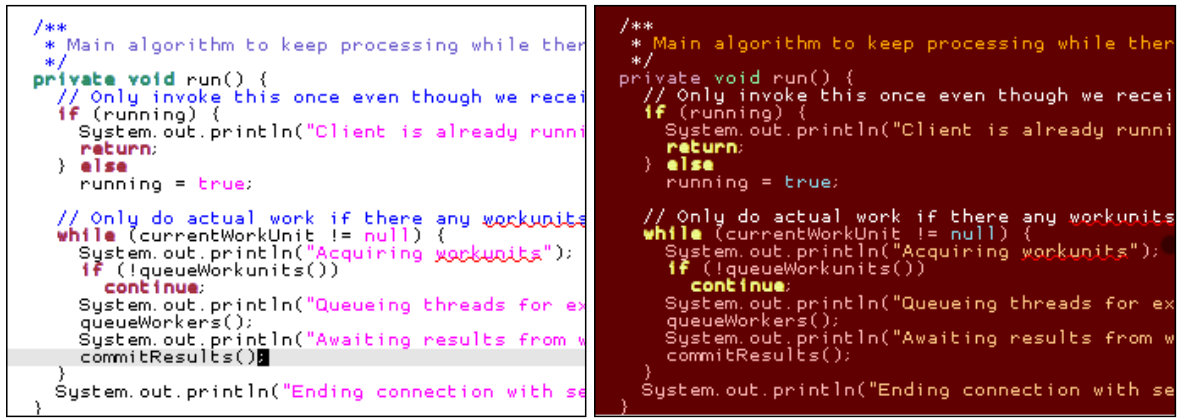
\includegraphics[scale=0.4]{./images/page22.png}
\end{center}

\subsection{个性化高亮}
\label{subsec:personal_highlighting}
在 Vim 中, 与高亮相关的最关键的技术是 \newterm{匹配} (\newterm{matching}).

通过匹配, Vim 几乎可以标记字母, 单词, 数值, 语句, 和文本行的任意一种组合.
用户甚至可以决定如何标记它们 (例如 用红色标记错误, 用绿色标记重点内容).

匹配通过下面这个命令完成:
\begin{vimcmdform}
\texttt{:match }\textit{group}\texttt{ /}\textit{pattern}\texttt{/}
\end{vimcmdform}
命令带有两个参数, 第一个参数是高亮文本时使用的色彩组的名字.
\begin{warning}
    配色方案影响的是全部的颜色设置, 而色彩组只是背景色 (或前景色) 的一个比
    较小的组合, 用户可以将其应用到某个方面, 比如匹配. 当 Vim 启动时, 根据
    所选择的配色方案, 大量的色彩组被设置成某个默认值.

    为了查看所有的色彩组, 执行 \texttt{:so \$VIMRUNTIME/syntax/hitest.vim}.
\end{warning}
\marginpar{23}
第 2 个参数是待匹配的模式. 模式是一个正则表达式, 可以很简单, 也可以极其
复杂 --- 取决于用户想要匹配什么样的内容. 匹配命令的一个比较简单的例子是:
\begin{vimcode}
:match ErrorMsg /^Error/
\end{vimcode}
\begin{center}
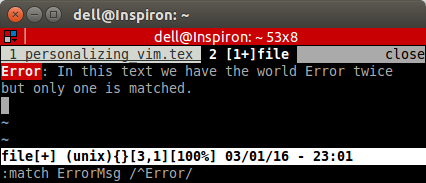
\includegraphics[scale=0.7]{./images/page23.png}
\end{center}

这个命令查找位于行的开始位置的单词 \textit{Error} (带有脱字符\ \texttt{ \^}),
如果找到了一个匹配, 就把匹配的文本用色彩组 \texttt{ErrorMsg} 的颜色
标记起来 (通常是红底白字).

如果读者不太喜欢已有的色彩组, 也可以自己定义一个, 定义色彩组的命令是:
\begin{vimcode}
:highlight MyGroup ctermbg=red guibg=red gctermfg=yellow
        guifg=yellow term=bold
\end{vimcode}
这个命令创建了一个名为 \file{MyGroup} 的色彩组, 红底黄字, 在控制台 (Vim)
和 GUI (Gvim) 环境下都是如此. 用户可以根据自己的喜好, 修改下列选项:

\begin{center}
\begin{tabular}{ll}
    \hline
    \texttt{ctermbg}    & 控制台环境下的背景色 \\
    \texttt{guibg}      & Gvim 环境下的背景色 \\
    \texttt{ctermfg}     & 控制台环境下的文本颜色 \\
    \texttt{guifg}      & Gvim 环境下的文本颜色 \\
    \texttt{gui}        & Gvim 环境下的字体格式 \\
    \texttt{term}       & 控制台环境下的字体格式 (比如粗体: bold) \\
    \hline
\end{tabular}
\end{center}

如果使用了已有的色彩组的名字, 那么在接下来的会话中如果用到了该色彩组,
所使用的将会是修改后的效果.

使用匹配命令时, 给定的模式会一直匹配下去, 直到执行一个新的匹配, 或者执行
下列命令:
\begin{vimcode}
:match NONE
\end{vimcode}
\marginpar{24}
匹配命令一次只能匹配一个模式, 但是 Vim 另外提供了 2 个命令用于一次匹配至
多 3 个模式. 命令很容易记忆:
\begin{vimcode}
:2match
:3match
\end{vimcode}
读者也许想知道这些匹配命令应该在什么样的情况下使用, 因为在平时的话这些命令
没什么大用处. 这里有一些例子, 它们展示出了匹配的强大之处.

\subsubsection{示例 1: 用彩色标记某列后面的文字}
\label{subsubsec:mark_color_characters_after_a_certain}
在写邮件时, 一条比较常见的规则是一行的长度不能超过 74 个字符 (在某些古老
的编程语言中, 同样存在这样的规则). 在这种情况下, 当用户在一行内写出的字符
数超过某个上限时, 如果 Vim 能够发出提醒那就再好不过了.

下面这个命令就可以完成上面提到的功能:
\begin{vimcode}
:match ErrorMsg /\%>73v.\+/
\end{vimcode}
执行该命令后, 一行内的第 73 个字符之后的那些字符都会被标记成错误. 匹配命令
中含有一个正则表达式, 这个表达式可以拆成:
\begin{center}
\begin{tabular}{ll}
    \hline
    \verb'\%>'  & 匹配该列之后的内容, 列号紧跟在尖括号的右边 \\
    \verb'73'   & 列号  \\
    \verb'v'    & 只能工作在可见的列上面 \\
    \verb'.\+'  & 匹配一个或多个任意的字符 \\
    \hline
\end{tabular}
\end{center}
\begin{center}
    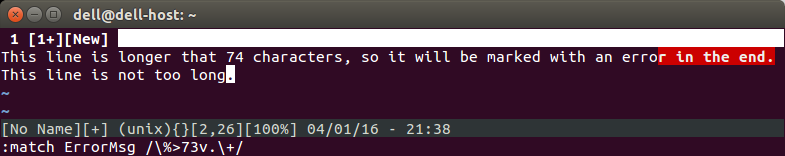
\includegraphics[scale=0.6]{./images/page24.png}
\end{center}
\marginpar{25}
\subsubsection{示例 2: 标记代码中未被用作缩进的制表符}
\label{subsubsec:mark_tabs_not_used_for_indentation_in_code}
编码时, 一条很重要的规则是制表符只被用作缩进代码, 其他地方则不允许使用制表
符. 然而, 对某些人来说常常会忘记该规则. 现在, 只需要一条简单的匹配命令, 就
可以时刻提醒着程序员.

下面这条命令把所有的, 不在行的开始位置上的制表符用错误信息的颜色标记出来:
\begin{vimcode}
:match ErrorMsg /[^\t]\zs\t\+/
\end{vimcode}
执行完该命令后, 程序员就可以时刻知道编码是否违反了规则 --- 把制表符用在了
代码内部. 把命令分解开来看, 它由下列这几个部分组成:
\begin{center}
    \begin{tabular}{ll}
        \hline
        \verb'[^'   & 字符组的开始标记, 组中的字符将不会被匹配到 \\
        \verb'\t'   & 制表符 \\
        \verb']'    & 字符组的结束标记 \\
        \verb'\zs'  & 一个宽度为 0 的匹配, 它把 ``匹配'' 置于一行的开始,
        并忽略任意的空格 \\
        \verb'\t\+' & 匹配一个或多个制表符 \\
        \hline
    \end{tabular}
\end{center}

\begin{center}
    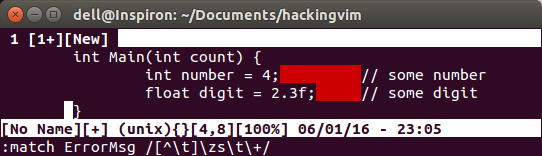
\includegraphics[scale=0.8]{./images/page25.png}
\end{center}

这个命令的意思是: 匹配所有的, 不在行的开始位置上的制表符 (忽略任意的空格).

如果你想用空格来缩进代码, 而不是制表符, 为了检查代码, 只需要把命令改成:
\begin{vimcode}
:match ErrorMsg /[\t]/
\end{vimcode}
这条命令的意思是: 匹配所有的制表符.
\marginpar{26}
\subsubsection{示例 3: 检查IP地址的有效性}
\label{subsubsec:preventing_errors_caused_by_ip_addresses}

如果用户需要在文本中写上大量的 IP 地址, 难免会出现错误 (例如
123.123.123.256). 为了防止出现这种情况, 可以把以下命令添加到文件
\file{vimrc} 中:
\begin{vimcode}
match errorMsg /\(2[5][6-9]\|2[6-9][0-9]\|[3-9][0-9][0-9]\)[.]
               \[0-9]\{1,3\}[.][0-9]\{1,3\}[.][0-9]\{1,3\}\|
               \[0-9]\{1,3\}[.]\(2[5][6-9]\|2[6-9][0-9]\|\
                \\ \[3-9][0-9][0-9]\)[.][0-9]\{1,3\}[.][0-9]
                \\{1,3\}\|\[0-9]\{1,3\}[.][0-9]\{1,3\}[.]\(2[5]
                \\ \[6-9]\|\2[6-9][0-9]|[3-9][0-9][0-9]\)[.][0-9]\{1,3\}
             \\|[0-9]\{1,3\}[.][0-9]\{1,3\}[.][0-9]\{1,3\}[.]
             \\(2[5][6-9]\|2[6-9][0-9]\|\[3-9][0-9][0-9]\)/

\end{vimcode}
相对于问题来说, 解决方法似乎有点太复杂了, 但请记住, 即使这条命令只能帮助你
一次, 但也值得把它加到配置文件.
\begin{warning}
从另一方面来看, 如果想匹配有效的 IP 地址, 执行:
\begin{vimcode}
:match Todo /\(\(25[0-5]\|2[0-4][0-9]\|[01]\?[0-9]
                [0-9]\?\)\.\)
                \\ \{3\}\(25[0-5]\|2[0-4][0-9]\|[01]\?
                [0-9][0-9]\?\)/
\end{vimcode}
\end{warning}

\section{更丰富的状态行}
\label{sec:a_more_informative_status_line}
在 Vim 窗口的底部, 读者会发现两样东西:
\begin{itemize}
    \item 命令行缓冲区 (输入命令的地方)
    \item 状态行
\end{itemize}
在默认的配置中, Vim 的状态行非常简单, 信息量也比较少. 状态行的右边显示
的是光标当前所在位置的行号与列号, 左边则是当前打开着的文件名 (如果有的话).

当执行 Vim 命令时, 状态行就会消失, 取而代之的是命令行缓冲区. 如果所执行的
命令带有输出信息, 那么这些信息就会出现在状态行的右侧.
\marginpar{27}
对于简单的文本编辑来说, 这样的状态行已经足够用了. 但是, 如果用户需要天天使用
Vim 来处理不同格式的文件, 那么一条信息量丰富的状态行将会提供很大的帮助.

这一节将会通过几个例子, 说明如何利用简单的办法来配置状态行, 使它
具有更丰富的信息.

配置状态行的命令具有形式:
\begin{vimcmdform}
\texttt{:set statusline}\ \ \textit{format}
\end{vimcmdform}
命令中的 \textit{format} 表示一个格式字符串 (就像 C 程序的 \texttt{printf}),
它描述了状态行的显示格式.

键入 \texttt{:help 'statusline'}, 打开 Vim 的帮助系统, 读者将会看到状态行
可以包含相当多的信息, 其中有些信息在日常工作中非常有用.

笔者的状态行信息包括:
\begin{itemize}
    \item 正在编辑的文件名
    \item 正在编辑的文件的格式 (比如 Dos, Unix)
    \item 文件类型
    \item 光标所在位置的字符的 ASCII 码值与十六进制值
    \item 光标所在的行号与列号
    \item 文件的长度 (以行为单位)
\end{itemize}
下面的命令可以让读者的 Vim 状态行包含上面提到的所有信息:
\begin{vimcode}
:set statusline=%F%m%r%h%w\ [FORMAT=%{&ff}]\ [TYPE=%Y]\ [ASCII=\%03.3b]\
 [HEX=\%02.2B]\ [POS=%04l,%04v]\ [%p%%]\ [LEN=%L]
\end{vimcode}
我在每一种信息的左右两边都加上了中括号, 这样做就更容易区分彼此. 加中括号只是为
了增加一些视觉效果, 如果不喜欢的话可以直接删掉.

\begin{center}
    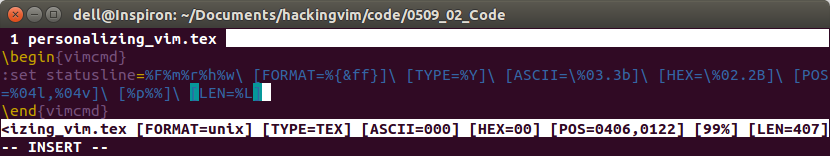
\includegraphics[scale=0.55]{images/page27.png}
\end{center}
\marginpar{28}
然而, 如果在安装 Vim 后没有做过多的配置, 即使执行了上面的状态行命令, 用
户也看不到状态行有什么变化. 这是因为默认情况下 Vim 根本就不会显示状态行,
它只会显示命令行缓冲区及其一小部分信息. 为了让 Vim 显示出真正的状态行, 用户
必须把下面这条命令添加到 \file{vimrc} 文件. 这条命令确保状态行始终显示在
倒数第 2 行的位置上:
\begin{vimcode}
:set laststatus=2
\end{vimcode}
执行完该命令后, 读者就会发现命令行缓冲区有了自己的位置: 窗口的最后一行. 通过
这条命令就可以保证状态行始终拥有自己的显示位置, 而用户也就能一直看到文件的
相关信息. 当然, 状态行会占据编辑区的一部分空间, 但是是否显示状态行由用户来
决定. 下面这条命令关闭状态行, 直到当前会话结束:
\begin{vimcode}
:set laststatus=0
\end{vimcode}

\section{切换菜单与工具条}
\label{sec:toggle_menu_and_toolbar}
如果用户是在控制台中使用 Vim, 就会逐渐习惯没有菜单与工具条的窗口. 但是如果用
的是 Gvim, 就会发现窗口界面提供了菜单与工具条.

许多人认为应该把额外的空间分配给更重要的文本使用, 而不是菜单与工具条. 如果
读者也是这么认为的, 那么读者可能希望在使用 Gvim 时, 移除菜单与工具条. 然而, 某
些脚本在菜单中增加许多有用的功能, 而这些功能也只能通过菜单来使用. 解决办法是
根据实际需要, 随时切换菜单与工具条.

下面的代码把 Gvim 的组合键 \key{Ctrl+F2} 映射到菜单与工具条的切换操作上,
如果读者喜欢这个功能的话, 可以把代码写到 \file{vimrc} 中.
\begin{vimcode}
map <silent> <C-F2> :if &guioptions =~# 'T' <Bar>
                         \set guioptions-=T <Bar>
                         \set guioptions-=m <bar>
                    \else <Bar>
                         \set guioptions+=T <Bar>
                         \set guioptions+=m <Bar>
                      \endif<CR>
\end{vimcode}
现在, 无论何时, 只要用户想关闭菜单与工具条, 好把空间留给文本, 只需要按下
\key{Ctrl+F2} 即可, 如果想它们了, 再按一下 \key{Ctrl+F2}, 它们就回来了.
\marginpar{29}
如果用户希望一直隐藏菜单或工具条, 只需要在 \file{vimrc} 中添加下面两个命令
中的一个即可.

为了完全移除菜单, 添加:
\begin{vimcode}
:set guioptions-=m
\end{vimcode}

为了完全移除工具条, 添加:
\begin{vimcode}
:set guioptions-=T
\end{vimcode}

\begin{warning}
    GUI 的其他设置可以通过命令 \texttt{set guioptions} 完成, 更多的信息可以
    参考\texttt{:help 'guioptions'}.
\end{warning}

\section{添加自定义菜单与工具条按钮}
\label{sec:adding_your_own_menu_and_toolbar_buttons}
如果使用的是 Gvim, 那么用户可以把经常用到的功能加到菜单中. 也许用户并不总
是需要通过菜单来使用某项功能, 但是如果忘记了具体的操作步骤, 还可以通过
菜单来完成. 如果用户确实需要快速地执行某个功能, 还可以把它直接加入到 Gvim
的工具条中.

这一节讨论如何在 Gvim 中制作菜单, 以及如何往工具条中加入额外
的按钮. 先从构造菜单开始.

\subsubsection{添加菜单}
\label{subsubsec:adding_a_menu}
简单来说, 为了构造一个菜单, 只需要为菜单中的每一个菜单项执行对应的命令即可.
只要遵循良好的命名规则, 用户就可以得到一个使用方便, 功能齐全的菜单.
\marginpar{30}
先从一个小例子开始, 假设用户想新增一个菜单, 比如缓冲区菜单.

\begin{center}
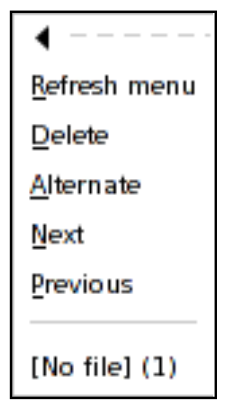
\includegraphics[scale=0.42]{./images/page30.png}
\end{center}

需要用到的命令是:
\begin{vimcmdform}
\texttt{:menu}\ \ \textit{menupath}\ \ \textit{command}
\end{vimcmdform}
这个命令的工作方式类似于命令 \texttt{map}, 后者把命令映射到一个组合键, 而前
者是把命令映射到一个菜单项.

命令带有两个参数. 第 1 个参数是菜单项在菜单中的实际路径, 第 2 个参数是菜单项
被点击时所执行的命令. 举个例子, 假设用户想要在菜单项 \newterm{Tabs} 中, 添加
一个新菜单项 \newterm{Next}, 执行:
\begin{vimcode}
:menu Tabs.Next <ESC>:tabnext<cr>
\end{vimcode}
之后, 用户就有了一个新菜单项 \newterm{Tabs}, 它只有一个子菜单项 \newterm{Next}.
现在, 如果用户点击菜单项 \newterm{Next}, 就会执行:
\begin{vimcode}
:tabnext
\end{vimcode}
命令前面的 \texttt{<ESC>} 为的是让 Vim 切换到普通模式,
后面的 \texttt{<cr>} 是真正开始执行命令的地方. 如果漏掉了 \texttt{<ESC>}, 那么
命令就无法正常地工作. 另外一种办法是根据当前的模式, 在命令前添加特定
的菜单项, 为此, Vim 提供了几个 \texttt{:menu} 的替代命令:
\begin{itemize}
    \item \texttt{:nmenu} 用于 \newterm{普通}(\newterm{Normal}) 模式
    \item \texttt{:imenu} 用于 \newterm{插入}(\newterm{Insert}) 模式, 前置
        \verb'^O'
    \item \texttt{:vmenu} 用于 \newterm{可视}(\newterm{Visual}) 模式, 前置
        \verb'^C', 后置 \verb'^\^G'
    \item \texttt{:cmenu} 用于 \newterm{命令行}(\newterm{Command-line}) 模式,
        前置 \verb'^C', 后置 \verb'^\^G'
    \item \texttt{:omenu} 用于 \newterm{操作挂起} (\newterm{OP-pending})
        模式, 前置 \verb'^C', 后置 \verb'^\^G'
\end{itemize}
\marginpar{31}
前置部分 (\verb'^O' 与 \verb'^C') 把 Vim 切换到普通模式.

\verb'^O' (\key{Ctrl+O}) 专门用于插入模式, 因为它会在执行完命令之后让编辑器
重新回到插入模式.

\verb'^\^G' (\key{Ctrl+\textbackslash}, \key{Ctrl+G}) 用于这样一种特殊情况:
全局插入模式被设置为真, 并且 Vim 把插入模式作为默认模式 (此时 Vim
是无模式的), 此时, 它们就可以把模式还原成原来的样子.
\begin{warning}
没必要为每一种模式创建一个同样的菜单项, 这时候只需要使用下面这个命令即可:
\begin{vimcmdform}
\texttt{:amenu}\ \ \textit{menu-path}\ \ \textit{command}
\end{vimcmdform}
这个命令可以根据当前的模式, 设置正确的前置命令与后置命令.
\end{warning}

现在开始创建新菜单 \newterm{Tabs}, 并添加几个新菜单项与功能. 执行了
下面这些命令后, 新菜单就有点像 \newterm{Buffers} 菜单了:
\begin{vimcode}
:amenu Tabs.&Delete :confirm tabclose<cr>
:amenu Tabs.&Alternate :confirm tabn #<cr>
:amenu <silent> Tabs.&Next :tabnext<cr>
:amenu <silent>Tabs.&Previous :tabprevious<cr>
\end{vimcode}
细心的读者会发现这些命令之中又多了点新东西.

第一个是 \texttt{<silent>}, 它可以阻止命令执行过程中, 命令的内容被回显到命令行
缓冲区. 当然, 这个功能只是装饰性的, 相比之下, 菜单路径中的 \verb'&' 就实
用多了. 把字符 \verb'&' 加在菜单路径的最后一个部分的某个字母之前, 就可以为该
菜单项定义一个快捷键. 有了快捷键, 定位并执行菜单项就可以更加方便.
\begin{center}
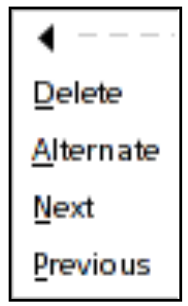
\includegraphics[scale=0.42]{./images/page31.png}
\end{center}
\marginpar{32}
假设用户想通过执行菜单项 \newterm{Tabs | Next} 来切换到下一个标签页, 现在,
只需要按下 \key{Alt + T + N} 即可. \key{Alt + T} 打开 \newterm{Tabs}, 再
按 \key{N} (之所以是 \key{N}, 是因为 \verb'&' 放在 \texttt{Next} 的
\texttt{N} 的前面) 来执行 \newterm{Next}. 如果有其他的菜单项使用了相同的
快捷键字母, 只需要一直按 \key{Alt} 就可以遍历所有的菜单项.
\begin{warning}
    如果用户希望下拉菜单的各项之间用一条横线分开, 可以使用 \texttt{SEP}
    (针对菜单项) 或 ``\texttt{:}'' (针对命令):
\begin{vimcode}
:amenu Tabs.-SEP-:
\end{vimcode}
用户创建的菜单仅对当前会话有效, 如果想要让菜单在下一次启动 Vim 时仍然存在,
可以把菜单的创建命令写到 \file{vimrc} 中 (写到 \file{vimrc} 的命令不需要前
面的冒号 \texttt{:}).
\end{warning}
现在已经有了一个简单的 \newterm{Tabs} 菜单, 看起来有点像菜单
\newterm{Buffers}. 不过它还不具备 \newterm{Buffers} 菜单所拥有的列出活动
缓冲区的功能. 缓冲区可以对用户隐藏起来, 而标签页肯定是可见的, 如果读者知道
这点, 就会明白这个功能对标签页来说没什么用处. 换句话说, 用户看见的标签页
就是当前编辑器中所有的标签页, 而且它们的名字都显示在标签的标题栏中.

一个 \newterm{Personal} 菜单可以用来完成许多有趣的事情. 如果用户需要处理多种
类型的文件, 甚至可以启动时为某个特定的文件类型创建菜单, 或者是在同一个菜单
下, 为不同的文件类型搭配不同的子菜单.

只需要遵循菜单路径的命名规范就可以创建出子菜单. 于是, 如果用户想要的菜单是
\newterm{Tabs | Navigation | Next}, 只需要用菜单路径
\texttt{Tabs.Navigation.\&Next} 来添加子菜单项 \newterm{Next}.

\subsubsection{添加工具条图标}
\label{subsubsec:adding_toolbar_icons}

既然已经知道了如何创建菜单, 那么给工具条添加自定义的图标就容易多了.
事实上, Vim 把工具条看作是带有特殊名字的菜单. 因此, 给工具条添加图标就像是
给菜单添加菜单项.

对于工具菜单, 为了给它添加一个子项目, 需要使用以 \texttt{ToolBar} 开始的
菜单路径. 为了给工具条添加一个用于执行命令 \texttt{:buffers} (列出打开的
缓冲区) 的子项目, 用户需要执行命令:
\begin{vimcode}
:amenu icon=/path/to/icon/myicon.png ToolBar.Bufferlist :buffers<cr>
\end{vimcode}
\marginpar{33}
当然, 用户必须把图标文件放在某个目录中, 并在命令中给出这个目录.

图标文件的存放目录通过参数 \texttt{icon} 传递给命令 \texttt{amenu}. 如果只
给出了文件名, 而没有给出路径, 那么 Vim 就会在运行时路径的 \texttt{bitmaps/}
目录下搜索图标文件 (运行时路径可以通过 \texttt{:echo \$VIMRUNTIME}
命令获取). 受支持的图标类型依赖于系统.

到现在为止就大功告成了! 执行完命令之后, 用户就可以看到他的图标出现在了工具
条中, 而且处在已有图标的最靠右的位置上. 如果点击该图标, Vim 就会执行命令
\texttt{:buffers}, 显示缓冲区列表.

和菜单一样, 可以通过特定于模式的菜单命令 \texttt{imenu}, \texttt{vmenu},
\texttt{cmenu} 等, 使得工具按钮只会在特定的模式下才会显示出来.

\begin{warning}
默认情况下, 新增的菜单或按钮图标处在已有的菜单或图标的右边, 可以通过优
先级来改变默认行为. 更多的信息请参考 \texttt{help menu-priority} 与
\texttt{:help sub-menu-priority}.
\end{warning}

\section{修改标签页}
\label{sec:modifying_tabs}
Vim 从 7.0 开始支持标签页. 标签页与其他应用程序中的标签不太一样 --- 在
Vim 中, 它是组织打开文件的一种方式. 每一个标签都可以包含若干个缓冲区,
甚至多个窗口.

有了标签页之后, 原来的针对所有缓冲区或窗口的命令 (例如 \texttt{:bufdo},
\texttt{:windo} 和 \texttt{:ball}) 将仅限于当前标签的窗口或缓冲区.

一般情况下, 所有的标签页以一种标签列表的形式呈现在窗口的上方 (就在编辑区
之上). 每一个标签页都有一个标签, 默认是处于当前活动缓冲区的文件名. 如果
一个标签页中同时打开了多个窗口, 那么标签也会显示窗口的数量.
\begin{center}
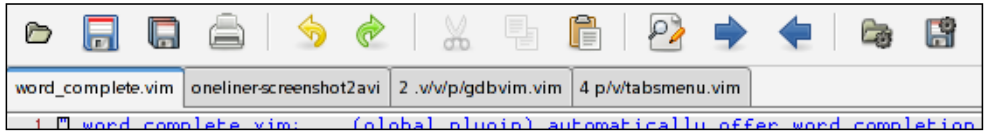
\includegraphics[scale=0.48]{./images/page33.png}
\end{center}
\marginpar{34}
有时候用户希望标签页的标签能提供更多的信息, 比如, 如果用户需要为每一个
项目建一个标签页, 要是能根据项目的名称来对标签页进行命名的话, 那就方便
多了.
\begin{center}

\includegraphics[scale=0.48]{./images/page34-1.png}
\end{center}
设置标签名的方法与状态行 (见 \ref{sec:a_more_informative_status_line} 节)
非常类似. 但是在这里设置的是 \texttt{tabline} 的属性, 而不是
\texttt{statusline}:
\begin{vimcmdform}
\texttt{:set tabline}\ \ \textit{tabline-layout}
\end{vimcmdform}
\begin{center}

\includegraphics[scale=0.48]{./images/page34-2.png}
\end{center}
如果是 Gvim, 则是
\begin{vimcode}
:set guitablabel
\end{vimcode}

虽然 \texttt{tabline} 的设置方法类似于 \texttt{statusline}, 但是前者会
更麻烦一点. 麻烦的主要原因在于用户必须时刻注意标签页是否处于活跃状态.
先从 Vim 的一个小例子开始.

如果标签页过多, 标签就会占据太多的空间, 尤其是当它们包含了当前活跃缓冲区
的完整文件名时. 我们希望只显示活跃缓冲区文件名的前 6 个字母, 而且当前
活跃的标签名以红底白字的方式呈现, 就像错误信息那样.

下面的 Vim 脚本程序完成的正是这个功能 (关于如何编写 Vim 脚本程序见第
\ref{chap:basic_vim_scripting} 章).
\begin{vimcode}
function ShortTabLine()
 let ret = ''
 for i in range(tabpagenr('$'))
   " select the color group for highlighting active tab
     if i + 1 == tabpagenr()
     let ret .= '%#errorMsg#'
   else
     let ret .= '%#TabLine#'
    endif

    " find the buffername for the tablabel
       let buflist = tabpagebuflist(i+1)
       let winnr = tabpagewinnr(i+1)
       let buffername = bufname(buflist[winnr - 1])
       let filename = fnamemodify(buffername,':t')
    " check if there is no name
\end{vimcode}
\marginpar{35}
\begin{vimcode}
    if filename == ''
      let filename = 'noname'
    endif
    " only show the first 6 letters of the name  and
    " .. if the filename is more than 8 letters long
    if strlen(filename) >=8
        let ret .= '['. filename[0:5].'..]'
    else
         let ret .= '['.filename.']'
    endif
 endfor

 " after the last tab fill with TabLineFill and reset tab page #
  let ret .= '%#TabLineFill#%T'
  return ret
endfunction
\end{vimcode}

现在, 需要把函数添加到 \file{vimrc}, 除此之外, 还要增加一行设置
\texttt{tabline} 的命令, 具体的设置命令是:
\begin{vimcode}
:set tabline=%!ShortTabLine()
\end{vimcode}
命令的执行结果是产生了一个更加紧凑的标签列表, 下面是效果截图:
\begin{center}

\includegraphics[scale=0.45]{./images/page35.png}
\end{center}

在 Gvim 中设置 \texttt{tabline} 的方法稍有不同, 不过基本思想是一样的. 然而
在 GUI 中, 用户不必考虑活跃标签的颜色, 也不必担心某个标签当前是否处于活跃
状态 --- 这些都是 GUI 自己需要考虑的东西.

于是, 可以对函数 \texttt{ShortTabLine()} 进行简化 --- 只需要设置标签
名即可:
\begin{vimcode}
function ShortTabLabel()
 let bufnrlist = tabpagebuflist(v:lnum)
 " show only the first 6 letters of the name + ..
 let label = bufname(bufnrlist[tabpagewinnr(v:lnum) - 1])
 let filename = fnamemodify(label,':h')
 " only add .. if string is more than 8 letters
  if strlen(filename) >=8
     let ret=filename[0:5].'..'
  else
    let ret = filename
 endif
     return ret
 endfunction
\end{vimcode}
\marginpar{36}
再把 \texttt{guitablabel} 的属性设置成函数的输出:
\begin{vimcode}
:set guitablabel=%{ShortTabLabel()}
\end{vimcode}
命令的执行效果是:
\begin{center}
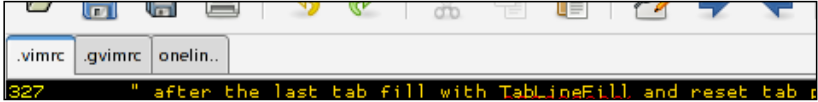
\includegraphics[scale=0.5]{./images/page36}
\end{center}

\begin{warning}
如果用户想要完全移除 Gvim 的标签栏, 执行 \texttt{:set showtabline=0}
(把 \texttt{showtabline} 设置成 1 则会重新显示标签栏).
\end{warning}

现在, 我们已经拥有了只含有有限信息的标签, 但还是希望能从其他地方
得到信息, 为了完成这个功能需要用到一个小技巧 --- 使用工具提示.

工具提示的优点是当用户没有激活它们时 (例如, 把鼠标移动到标签页的位置上,
就有可能激活标签页的提示信息),
就不会看到这些提示信息. 使用这种方法就可以做到在不填满整个编辑器的情况下,
仍然可以获取到信息.

为了给一个标签页设置工具提示, 需要使用下面的命令:
\begin{vimcode}
:set guitabtooltip
\end{vimcode}
用户需要把它设置成当鼠标经过标签名时, 希望显示出来的信息.

为了测试, 可以先输入一条简单的提示信息:
\begin{vimcode}
:set guitabtooltip='my tooltip'
\end{vimcode}
现在, 工具提示中就可以显示一条静态消息, 但我们需要更多的信息. 文件的路径部
分已经从标签中移走了, 但是有时候仍然需要这个信息. 有了工具提示,
就可以把路径信息显示在工具提示中:
\begin{vimcode}
:set guitabtooltip=%!bufname($)
\end{vimcode}

函数可以根据标签的不同, 显示对应的提示信息. 这里, 我们构造了一个小函数, 用
于显示用户会在标签中看到的所有信息, 不过用了一种更加有条理的方式显示出来:
\begin{vimcode}
function! InfoGuiTooltip()
    "get window count
\end{vimcode}
\marginpar{37}
\begin{vimcode}
    let wincount = tabpagewinnr(tabpagenr(),'$')
    let bufferlist=''
   "get name of active buffers in windows
    for i in tabpagebuflist()
        let bufferlist .= '['.fnamemodify(bufname(i),':t').'] '
    endfor
    return bufname($).' windows: '.wincount.' ' .bufferlist ' '
endfunction
\end{vimcode}
然后执行:
\begin{vimcode}
:set guitabtooltip=%!InfoGuiTooltip()
\end{vimcode}
下面这张截图展示了工具提示在 Gvim 中的效果:
\begin{center}
    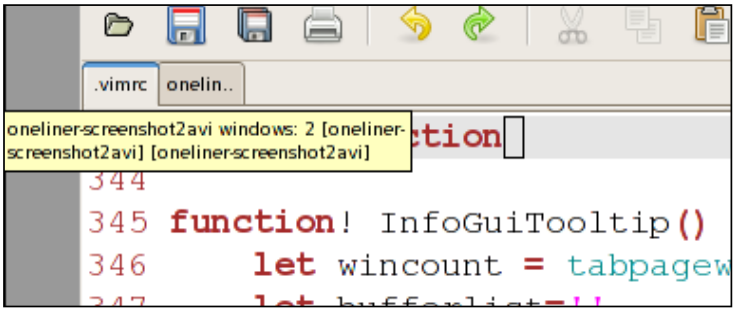
\includegraphics[scale=0.4]{images/page37.png}
\end{center}

用户还可以想到许多其他有趣的用法, 来使用标签与工具提示所提供的功能, 有了前
面的示例, 用户就可以自己动手来实现它们了.

\section{工作区定制}
\label{sec:work_area_personalization}

这一节介绍一些专门针对 Vim 编辑区的设置内容, 之所以介绍这些,
是因为当用户使用 Vim 编辑文本或代码时, 它们可以提高用户的工作效率.

\subsection{为光标添加视觉效果}
\label{subsec:adding_a_more_visual_cursor}
有时候, 用户正在编辑的文件可能带有多种颜色的语法高亮, 这些颜色会干扰用户
追踪光标的位置, 如果可以标记出光标当前所在的行, 那就方便多了.

已经有很多人写过 Vim 脚本来解决这个问题, 但是绝大部分都没什么用 (主要
是因为太慢了, 当文本过长时, 滚动速度就难以接受). 直到 Vim 版本 7, 这个
问题才得以解决, 而且, 它还提供了两种可能的办法来追踪光标的位置.
\marginpar{38}
第一种办法是命令 \texttt{cursorline}, 它可以标记当前光标所在的行, 比如把
当前行的背景色设置成另一种颜色, 而且不会破坏原来的语法高亮. 为了打开它,
执行:
\begin{vimcode}
:set cursorline
\end{vimcode}
命令所使用的颜色由色彩组 \texttt{CursorLine} 定义, 用户可以它设置成任意一种
颜色或风格, 比如:
\begin{vimcode}
:highlight CursorLine guibg=lightblue ctermbg=lightgray
\end{vimcode}
关于色彩组的更多内容请参考 \ref{subsec:personal_highlighting} 节.

\begin{center}
    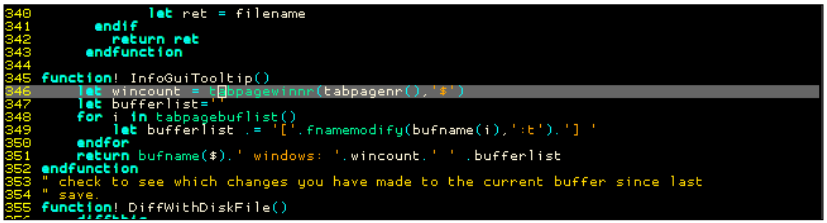
\includegraphics[scale=0.5]{./images/page38-1.png}
\end{center}

如果用户正在编辑的文件含有许多对齐的内容 (比如用制表符分隔的数据), 那么很自然
地就会用到:
\begin{vimcode}
:set cursorcolumn
\end{vimcode}

这个命令标记光标当前所在的列, 例如, 可以用另外一种颜色来标记.

和 \texttt{cursorline} 类似, 用户可以修改 \texttt{cursorcolumn} 的标记设置,
它的色彩组是 \texttt{CursorColumn}.

如果同时设置了 \texttt{cursorline} 与 \texttt{cursorcolumn}, 那么光标看起来
就像一对十字线, 这样就再也不用怕把它跟丢了.
\begin{center}
    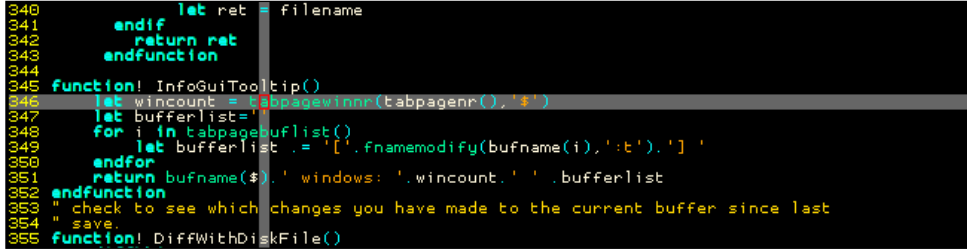
\includegraphics[scale=0.45]{./images/page38-2.png}
\end{center}
\marginpar{39}
\begin{warning}
虽然 \texttt{cursorline} 与 \texttt{cursorcolumn} 是在 Vim 本地实现的, 但是
仍然会影响文件的滚动速度.
\end{warning}

\subsection{添加行号}
\label{subsec:adding_line_numbers}
在编译或调试代码时, 错误信息通常会报告错误所在的行号, 为了定位到这一行, 用户
当然可以从第 1 行开始, 一行一行地往下数, 不过 Vim 提供了更为直接的办法. 只
需要执行 \texttt{:}\textit{XXX} (\textit{XXX} 表示行号), 用户就可以马上到达
第 \textit{XXX} 行.

另一种办法是在普通模式 (按下 \key{Esc} 就可以切换到普通模式) 下, 执行
\textit{XXX}\texttt{gg} 或 \textit{XXX}\texttt{G} (同样, \textit{XXX} 表示
行号). 但是, 如果能随时随地地看到行号可能会更加方便, 这时候就可以执行命令:
\begin{vimcode}
:set number
\end{vimcode}

执行完命令后, 编辑器就会在窗口的左边显示每一行的行号. 默认情况下行号占据 4
个空格的宽度, 3 个用于数字, 1 个用于空格. 这意味着行号所占据的宽度总是一样
的, 除非总行数超过了 999 行. 如果总行数超过了 999 行, 行号所占据的宽度就
会增加一列, 相应地, 文件内容就会右移一列.

当然, 用户可以修改行号占据的列宽, 相应的命令是:
\begin{vimcmdform}
\texttt{:set numberwidth=}\textit{XXX}
\end{vimcmdform}
把 \textit{XXX} 替换成你想要的列宽度.

\begin{warning}
    用户可能希望通过加大列宽度的值, 使得代码与行号之间的间距更大一些,
    但是这个配置无法通过 \texttt{numberwidth} 实现, 因为行号是右对齐的.
\end{warning}
\marginpar{40}

在下面的图片中, 读者可以看到: 当 \texttt{numberwidth} 的值增大时, 行号是如何
右对齐的.

\begin{center}

\includegraphics[scale=0.4]{./images/page40.png}
\end{center}

\begin{warning}
    用户可以通过修改色彩组 \texttt{LineNr} 来改变行号及其所在列的风格.
\end{warning}

\subsection{拼写检查}
\label{subsec:spell_checking_your_language}

这个道理谁都懂! 虽然人们对拼写都很在行, 但总会发生拼写错误或打错字的情况.
过去, 为了进行拼写检查 (文本内容已经写在了 Vim 中), 用户需要使用某种拼写检查
工具, 比如 Aspell 或 Ispell. 如果把拼写检查作为最后一项工作, 那么修改起来会
非常得累人, 除非你想过一会儿就检查一遍.

到了 Vim 版本 7, 这种麻烦的拼写检查方式终于可以结束了. 现在, Vim 内置了一个
拼写检查工具, 它支持的语言超过 50 种.

拼写检查工具会在用户输入单词的时候检查拼写的正确性, 所以如果有错误发生的话,
用户可以马上发现.

打开拼写检查的命令是
\begin{vimcode}
:set spell
\end{vimcode}
命令使用默认的语言 (英语) 打开拼写检查, 如果想要使用其他语言, 只需要把
\texttt{spelllang} 设置成该语言的代号即可. 比如:
\begin{vimcode}
:set spelllang=de
\end{vimcode}
\marginpar{41}
在这个命令中语言被设置为德语. 同一种语言可以用多种形式的格式来表达, 比如美式
英文可以写成:
\begin{itemize}
    \item \texttt{en\_us}
    \item \texttt{us}
    \item \texttt{American}
\end{itemize}

语言的名字甚至可以是专业名词, 比如 \texttt{medical}. 如果 Vim 无法识别用户
输入的语言名字, 那么在执行属性设置命令时, 它就会高亮显示无法识别的语言名字.

\begin{warning}
    如果把 \texttt{spelllang} 设置成某个还没有安装的语言, Vim 就会询问用户
    是否自动从 Vim 主页上下载对应的语言.
\end{warning}

对笔者个人来说, 我经常要用 Vim 同时处理不同的语言, 而且并不想每次都告诉 Vim
现在用的是什么语言.

对此 Vim 也有解决办法. 只要在设置属性 \texttt{spelllang} 时, 给它同时带上
多种语言即可 (语言之间用逗号分开), 这样 Vim 就可以用多种语言来进行语法检查.
\begin{vimcode}
:set spelllang=en,da,de,it
\end{vimcode}
Vim 将会按照顺序, 轮流根据每一种语言检查单词的拼写是否正确. 如果单词对某一种
语言来说是正确拼写的, 那它就不会被标记错误. 当然, 这就意味着如果有一个
单词的拼写本来是错误的, 可是碰巧它在另一种语言中是正确的, 那么它也不会被
当成错误, 这将会引入一个难以察觉的错误.

\begin{warning}
    用户可以到 Vim 的 FTP 站点 \url{ftp://ftp.vim.org/pub/vim/runtime/spell}
    上找到大量的语言包.
\end{warning}

Vim 与 Gvim 对错误单词的标记方法稍有不同.

在普通的 Vim 中, 拼写错误的单词使用色彩组 \texttt{SpellBad} 标记 (默认情况下
是红底白字).
\marginpar{42}

在 Gvim 中, 拼写错误的单词用红色的波浪线标记, 当然, 这也可以通过设置色彩组
来改变颜色 (关于如何设置色彩组见 \ref{subsec:personal_highlighting} 节).

\begin{center}
    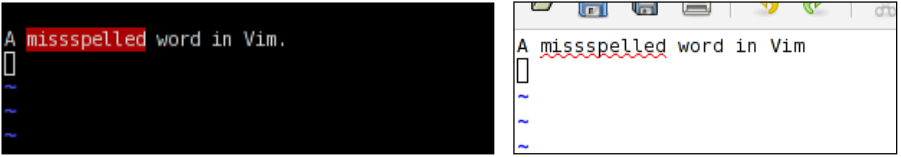
\includegraphics[scale=0.5]{./images/page42-1.png}
\end{center}

无论用户是在什么时候碰到拼写错误的单词, 都可以向 Vim 询问正确的拼写方式.
为此, 需要把光标置于单词中, 并切换到普通模式 (按 \key{Esc}), 然后按
\texttt{z=}.

\begin{center}
    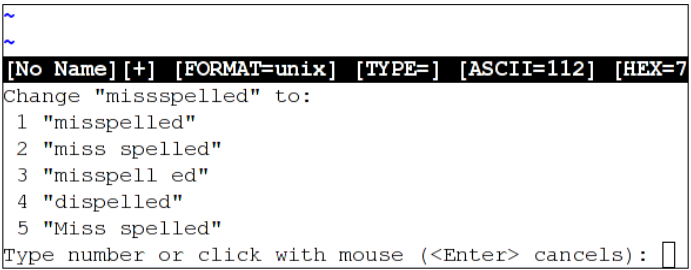
\includegraphics[scale=0.5]{./images/page42-2.png}
\end{center}

如果可能的话, Vim 将会猜测用户试图输入的单词的正确形式, 并给出一个候选列表.
在每个候选单词的前面都有一个数字, 如果其中有你想要的单词, 就输入单词前面的
数字或者单词本身, 然后按 \key{Enter}.

Vim 会给出一长串的候选单词, 除非用户把单词完全拼写错了, 否则的话, 单词的正
确形式应该就在候选单词的前 5 个中, 如果用户不想看到一长串的列表, 那么他就
可以用命令
\begin{vimcmdform}
\texttt{:set spellsuggest=}\textit{width}
\end{vimcmdform}
来限制列表的长度, 其中 \textit{width} 是列表的最大长度.
\marginpar{43}

\subsection{添加帮助性的工具提示}
\label{subsec:adding_helpful_tool_tips}

在 \ref{sec:modifying_tabs} 节, 我们学习了如何利用工具提示, 使得在占据较少
空间的情况下, 存放更多的信息, 以此为基础, 我们将把工具提示应用在编辑器的其中
地方.

编辑区是 Vim 中面积最大的部分, 所以, 为什么不利用工具提示, 在编辑区中添加
一些额外的信息呢?

在 Vim 中, 编辑区的工具提示称为 balloons, 只在当鼠标停在组成这个单词的
某个字符的上方时, 提示信息才会显示出来. 为了使用 balloons, 用户必须知道
下面这几个命令:
\begin{itemize}
    \item 第 1 个命令是在 Vim 中启用 balloons:
\begin{vimcode}
:set ballooneval
\end{vimcode}
    \item 第 2 个命令告诉 Vim 在显示信息之前需要等待多长时间 (默认是 600
    毫秒):
\begin{vimcode}
:set balloondelay=400
\end{vimcode}
    \item 最后一个命令是设置信息的内容:
\begin{vimcode}
:set balloonexpr="textstring"
\end{vimcode}
    信息的内容既可以是静态的文本字符串, 也可以是函数的返回值.
\end{itemize}

为了访问鼠标所在的位置的相关信息, Vim 提供了一些变量:
\begin{center}
\begin{tabular}{ll}
    \hline
    \texttt{v:beval\_bufnr} & 鼠标所在区域的缓冲区个数 \\
    \texttt{v:beval\_winnr} & 鼠标所在区域的窗口的个数 \\
    \texttt{v:beval\_lnum}  & 鼠标所在的行号 \\
    \texttt{v:beval\_col}   & 鼠标所在的列号 \\
    \texttt{v:beval\_text}  & 触发提示信息的字符所在的单词 \\
    \hline
\end{tabular}
\end{center}
\marginpar{44}
有了这些变量之后, 来看一些具体的例子.

\subsubsection{示例 1}
\label{subsubsec:example_1}

第 1 个例子基于 Vim 的帮助系统, 它展示了如何编写一个简单的函数, 用来显示
所有的变量.
\begin{vimcode}
function! SimpleBalloon()
   return 'Cursor is at line/column: ' . v:beval_lnum .
		\'/' . v:beval_col .
		\ ' in file ' .  bufname(v:beval_bufnr) .
		\ '. Word under cursor is: "' . v:beval_text . '"'
endfunction
set balloonexpr=SimpleBalloon()
set ballooneval
\end{vimcode}
脚本的运行结果是:
\begin{center}
    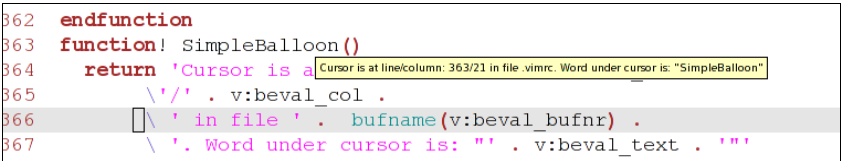
\includegraphics[scale=0.5]{./images/page44.png}
\end{center}

\subsubsection{示例 2}
\label{subsubsec:example_2}

现在来看一个更高级的例子, 这个例子把 balloons 应用到编辑区的特定区域上.
在这个例子中, 我们将会开发一个函数, 这个函数可以同时显示两种 balloons
信息:
\begin{itemize}
    \item 拼写错误的单词: 这个 balloons 信息给出候选单词.
    \item 折叠的文本: 这个 balloons 信息给出被折叠的文本的预览.
\end{itemize}

现在, 我们需要知道什么样的函数可以帮助判断鼠标是停在拼写错误的单词上,
还是停在一个折叠行 (这个折叠行代表了折叠后的多个文本行) 上.

为了判断单词的拼写是否错误, 需要打开拼写检查功能:
\begin{vimcode}
:set spell
\end{vimcode}
\marginpar{45}
打开后, 如果鼠标所在的单词有拼写错误, 被调用的内置拼写检查函数 ---
\texttt{spellsuggest()} --- 就会返回候选单词. 所以, 为了判断某个单词的拼写
是否有错, 只需要检查 \texttt{spellsuggest()} 的返回值即可. 不过有一点需要
注意, 即使单词没有拼错, \texttt{spellsuggest()} 也可能会返回候选单词.
为了解决这个问题, 在把单词交给 \texttt{spellsuggest()} 之前, 需要用另一个
函数过滤一下, 这个函数叫作 \texttt{spellbadword()}. 它的作用是把光标移动
到句子中第一个拼错的单词上, 然后再返回这个单词. 如果输入一个拼写正确
的单词, 那么它应该不返回任何信息. 如果没有单词被输送给
\texttt{spellsuggest()}, 那它就不会返回候选单词, 于是, 我们现在就可以检查
某个单词是否有拼写错误.

检查某个单词是否在一个折叠块中更简单. 以鼠标所在的行号作为输入参数,
调用函数 \texttt{foldclosed()} (回忆变量 \texttt{v:beval\_lnum}), 它会
返回鼠标所在的折叠块的第一行的行号, 如果不是折叠块, 就返回 \texttt{-1}.
换句话说, 如果 \texttt{foldclosed(v:beval\_lnum} 返回除了 \texttt{-1}
之外的其他值, 那么就在一个折叠块中.

把上面提到的所有内容都搜集起来, 就得到了下面这个函数:
\begin{vimcode}
function! FoldSpellBalloon()
  let foldStart = foldclosed(v:beval_lnum )
  let foldEnd   = foldclosedend(v:beval_lnum)
  let lines = []
  " Detect if we are in a fold
  if foldStart < 0
    " Detect if we are on a misspelled word
    let lines = spellsuggest( spellbadword(v:beval_text)[ 0 ], 5, 0 )
  else
    " we are in a fold
    let numLines = foldEnd - foldStart + 1
    " if we have too many lines in fold, show only the first 14
    " and the last 14 lines
    if ( numLines > 31 )
      let lines = getline( foldStart, foldStart + 14 )
      let lines += [ '-- Snipped ' . ( numLines - 30 ) . ' lines --' ]
      let lines += getline( foldEnd - 14, foldEnd )
    else
      "less than 30 lines, lets show all of them
      let lines = getline( foldStart, foldEnd )
    endif
  endif
  " return result
\end{vimcode}
\marginpar{46}
\begin{vimcode}
  return join( lines, has( "balloon_multiline" ) ? "\n" : " " )
endfunction

set balloonexpr=FoldSpellBalloon()
set ballooneval
\end{vimcode}

这些帮助性的 balloons 可以极大地提高用户的工作效率, 下面的图展示了折叠块
的预览效果:
\begin{center}
    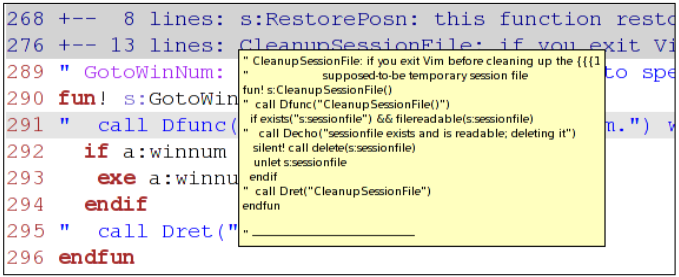
\includegraphics[scale=0.4]{./images/page46-1.png}
\end{center}

如果把它应用到一个拼写错误的单词上, 得到的就是:
\begin{center}
    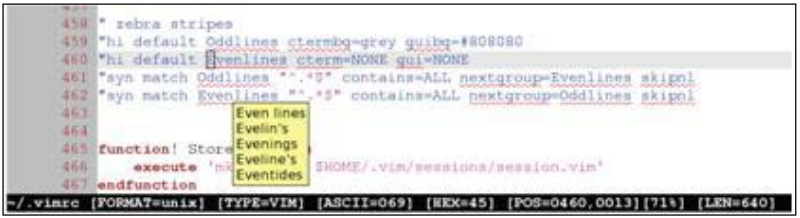
\includegraphics[scale=0.4]{./images/page46-2.png}
\end{center}

\begin{warning}
    在第 \ref{chap:production_boosters} 章, 读者将会学习到如何利用行
    的折叠来提高 Vim 的生产力.
\end{warning}

\subsection{使用缩写}
\label{subsec:using_abbreviations}

对于重复性工作很多人都深有体会, 但这种现象却恰恰是 Vim 想要极力避免的.
\marginpar{47}
Vim 的设计哲学是: 如果用户曾经为某件事物写过一次, 那就不需要再写第二次.
然而, 如果用户发现自己正在一次又一次地输入同一个内容, 那就说明他需要找到
一个更好的办法.

为了避免多次输入同一个内容, 用户可以使用 缩写 (abbreviations).

根据不同的使用模式, 可以使用以下三个命令来创建缩写:
\begin{itemize}
    \item \texttt{:abbreviate}: 创建在所有模式中均可使用的缩写
    \item \texttt{:iabbrev}: 创建只能在插入模式中使用的缩写
    \item \texttt{:cabbrev}: 创建只能在命令行中使用的缩写
\end{itemize}

上面所说的三个命令都需要两个参数 --- 文本的缩写形式与完整形式.

先用一个简单的例子来说明在什么情况下应该使用缩写.

\subsubsection{用缩写来快速插入地址}
\label{subsubsec:using_abbreviations_for_quick_address_insertion}
在过去的几年我更换了几次住所, 所以我的一个经常性的工作就是把新住址
告诉给别人. 为地址准备一个缩写并不会花上太多时间, 有了缩写之后, 就不用每
次都把整个地址都写出来.

命令的具体形式是:
\begin{vimcode}
:iabbrev myAddr 32 Lincoln Road, Birminham B27 6PA, United Kingdom
\end{vimcode}
每当我想要输入自己的地址时, 只需要键入 \texttt{myAddr}, 紧接着按一下空格
键, Vim 就会把 \texttt{myAddr} 自动地扩展为完整的地址.

Vim 非常聪明, 它可以判断用户是在输入一个缩写词, 还是仅仅在输入另一个单词
的某个部分, 所以它只会在输入缩写词并按了空格键之后, 才把缩写扩展为完整
的字符串. 如果在输完缩写词之后, 紧跟着的是一个普通的字母, 那么 Vim 就会知
道用户并不是在输入某个缩写词, 自然也就不会发生扩展. 有关缩写词 \texttt{abc}
的例子如下:
\begin{center}
\begin{tabular}{ll}
    \hline
    \texttt{abc<space>}     & 扩展 \\
    \texttt{abc<enter>}     & 扩展 \\
    \texttt{123abc<space}   & 不会扩展, 因为缩写词现在是某个单词的一部分 \\
    \texttt{abcd<space>}    & 不会扩展, 因为在缩写词后面紧跟着的是字母 \\
    \texttt{abc}            & 不会扩展, 除非接下来输入另一个特殊字符 \\
    \hline
\end{tabular}
\end{center}
\marginpar{48}

为了避免每次都执行一次缩写命令, 用户可以把它们放在 \texttt{VIMHOME} 的某个
文件中, 假设文件名就叫 \texttt{abbreviations.vim}, 然后在文件 \texttt{vimrc}
使用命令 \texttt{source} 来使能该文件 (需确保该文件是可读的):
\begin{vimcode}
:source $VIM/abbreviations.vim
\end{vimcode}

每当用户需要一个新的缩写词时, 可以先在编辑器中创建缩写词, 然后再把它加入到文件
\texttt{abbreviations.vim}.

也许读者已经意识到, 除了这些, 缩写可以应用在其他有趣的地方. 但无论如何,
这里有一些例子, 或许可以向你提供一些思路:
\begin{itemize}
    \item 纠正常见的拼写错误:
\begin{vimcode}
:iabbr teh the
\end{vimcode}
    \item 编程模版
\begin{vimcode}
:iabbr forx for(x=0;x<100;x++){<cr><cr>}
\end{vimcode}
    \item 更短的命令
\begin{vimcode}
:cabbr csn colorscheme night
\end{vimcode}
\end{itemize}

如果读者发现了一个新的缩写, 或许它看起来有点古怪, 刚开始用的时候还有点麻烦,
但是读者应该习惯这一点, 因为到最后将会发现, 它可以帮助你节省大量的时间.
用户唯一所要做的事就是把新的缩写加入到配置文件中, 然后再重新加载即可.

但是有时候缩写可能会比较恼人, 因为它自作聪明地扩展了用户并不希望扩展的单词.
比如, 用户有一个地址的缩写词是 ``addr'', 但是用户其实想写的是单词
``addressed''. 在这种情况下, 缩写功能会突然冒出来, 用户也很难轻易地写出他
所想要的单词.

一种解决办法是在插入单词之前调用一个函数, 该函数询问用户是否使用缩写
扩展功能.

该函数的一种实现是:
\begin{vimcode}
function! s:AbbrAsk(abbr,expansion)
    let answer = confirm("use the abbreviation '" . a:addr . "'?",
        "&Yes\n&No", 1)
    return answer ==  1 ? a:expansion : a:abbr
endfunction
\end{vimcode}
\marginpar{49}

函数需要两个参数, 第 1 个参数是缩写诩, 第 2 个参数缩写词扩展后的形式,
对我们的例子来说, 该函数的用法是:
\begin{vimcode}
:iabbrev <expr> addr <SID>AbbrAsk('addr', "your full address here")
\end{vimcode}

所以, 当用户写下 \texttt{addr} 时, Vim 会询问用户是否对缩写词进行扩展.

\subsection{修改按键绑定}
\label{subsec:modifying_key_bindings}

我们中的大部分人可能除了 Vim 之外, 还用过其他的编辑器, 正因为如此, 我们经常
需要用到一些特定的快捷键来完成不同的任务.

虽然 Vim 中的快捷键绑定在最开始设计时都是力求使用方便且快速, 但是在某些情况
下, 使用用户已经熟悉的快捷键可能会更快.

为了完成这个功能, Vim 几乎可以对任何一个单独的按键进行重新绑定.

这一节将会介绍在不同的模式下, 如何对 Vim 的按键绑定进行修改.

处理按键绑定的命令主要有:
\begin{itemize}
    \item \texttt{:map}  用于普通模式, 插入模式, 可视模式, 与命令行模式
    \item \texttt{:imap}  只能用于插入模式
    \item \texttt{:cmap}  只能用于命令行模式
    \item \texttt{:nmap}  只能用于普通模式
    \item \texttt{:vmap}  只能用于可视模式
\end{itemize}

每一个命令都需要两个参数, 第一个参数是被绑定的按键, 第二个参数是被绑定的命
令. 先看几个例子.

假设用户不太习惯在普通模式下用命令 \texttt{:w} 来保存文件, 因为你已经习惯了
\key{Ctrl-S}, 并且想继续使用下去.
\marginpar{50}
解决这个问题的一个映射可以是:
\begin{vimcode}
:map <C-s> :w<cr>
\end{vimcode}

注意命令中的 \texttt{<C-s>}, 这是组合键 \key{Ctrl+S} 在 Vim 中的表示方式.
除了 \texttt{C} (\key{Ctrl}), 用户还可以用 \texttt{A} (\key{Alt}) 或
\texttt{M} (\key{Meta}). 命令末尾的 \texttt{<cr>} 是真正执行命令的地方.
如果缺了它, 命令只会被显示在命令行中, 而不会被执行.

除了 \texttt{<cr>}, 还有其他的一些用来表示按键的特殊记号, 下面这张表显示了
比较常见的记号:
\begin{center}
    \begin{tabular}{ll}
        \hline
        按键        & 记号  \\
        \hline
        \texttt{<BS>}   & 退格 \\
        \texttt{<Tab>}   &  制表符 \\
        \texttt{<CR>}   & 回车  \\
        \texttt{<Enter>}   & 回车 \\
        \texttt{<Return>}   & 回车 \\
        \texttt{<Esc>}   & 转义 \\
        \texttt{<Space>}   & 空格 \\
        \texttt{<Up>}   & 方向键, 上 \\
        \texttt{<Down>}   & 方向键, 下 \\
        \texttt{<Left>}   & 方向键, 左 \\
        \texttt{<Right>}   & 方向键, 右 \\
        \texttt{<F1>} - \texttt{<F12>}  & 功能键, \texttt{F1} 到
            \texttt{F12} \\
        \texttt{\#1}, \texttt{\#2},...,\texttt{\#9}, \texttt{\#0}  & 功能键, 从
            \texttt{F1} 到 \texttt{F10} \\
        \texttt{<Insert>}   & 插入 \\
        \texttt{<Del>}   & 删除 \\
        \texttt{<Home>}   & 返回到行的开始 \\
        \texttt{<End>}   & 返回到行的结束 \\
        \texttt{<PageUp>}   & 下一页 \\
        \texttt{<PageDown>}   & 上一页 \\
        \hline
    \end{tabular}
\end{center}

如果用户只可能在插入模式下才会保存文件, 而且在保存之后想要继续在插入模式下
工作, 那就执行:
\begin{vimcode}
:imap <C-s> <esc>:w<cr>a
\end{vimcode}
\marginpar{51}

之后, \key{Ctrl+S} 就被映射成几个按键的组合. 首先, 按下 \texttt{<esc>}
(\key{Escape} 键), 使 Vim 从插入模式进入到普通模式. 然后, 使用
\texttt{:w<cr>} 完成实际的文件保存操作. 最后, 用 \texttt{a} 再回到插入模式,
并将光标移到行的末尾.

用户可以通过映射来适应大多数应用程序的标准的 复制/粘贴/剪切/保存 快捷键,
具体来说, 可以这样做:
\begin{vimcode}
" save file (ctrl-s)
:map <C-s> :w<cr>
" copy selected text (ctrl-c)
:vmap <C-c> y
" Paste clipboard contents (ctrl-v)
:imap <C-p> <esc>P
" cut selected text (ctrl-x)
:vmap <C-x> x
\end{vimcode}

如果是 Gvim, 甚至可以打开 \texttt{Save-as} 与 \texttt{Open} 的对话框:
\begin{vimcode}
" Open new file dialog (ctrl-n)
:map <C-n> :browse confirm e<cr>
" Open save-as dialog (ctrl-shift-s)
:map <C-S-s> :browse confirm saveas<cr>
\end{vimcode}

用户可能会遇到这样一种情况: 组合键的第一个按键已经绑定到了 Vim 的某个功能
上. 举个例子, 按键 \verb'$', 它的功能是把光标移到一行的末尾. 用户可能希望
为 \verb'$1' 新绑定一个功能, 为 \verb'$2' 绑定另一个功能, 如此等等. 具体的
形式是:
\begin{vimcode}
:map $1 :MyFunction1()<cr>
:map $2 :MyFunction2()<cr>
\end{vimcode}

现在, 如果用户按下了 \key{\$}, Vim 就会等待一秒, 等待另一个按键被按下,
如果在这一秒之内没有按键按下, Vim 就会执行原来的功能: 把光标移到一行的末尾.
相反, 如果在 1 秒之内用户按下了 \key{1}, Vim 就会执行函数
\texttt{MyFunction1()}.

有了按键映射功能, 用户就有了一个强大的工具来根据自己的需要, 对 Vim 进行
修改.

\begin{tips}
    关于映射的更多的帮助信息, 可以查看 Vim 的帮助系统: \texttt{:help
    key-mapping}.
\end{tips}
\marginpar{52}
\section{小结}
\label{sec:personalizing_vim_summary}

在这一章, 我们学习了如何根据自己的具体需求来配置 Vim.

首先学习了字体与配色方案的基本修改方法, 通过它们来修改 Vim 的外观.

接下来, 讨论了如何使用颜色来标记搜索匹配, 从而使得它们更容易被识别.

为了最大限度地利用 Vim, 用户通常将大部分的区域用于编辑, 而将小部分区域用于
其他功能. 因此, 我们介绍了如何配置状态行与标签列表, 使得它们占用更少的空间,
同时提供更多的信息.

虽然菜单栏与工具栏不是非常重要, 而且还会占用本来就有限的屏幕空间, 但是它们
仍然可以提供很大的用处. 在这一章, 学习了如何在菜单栏中添加自定义的菜单,
以及如何在工具栏中添加图标.

为了让编辑区更符合用户的需求, 可以对它进行许多修改. 这一章简单地讨
论了编辑区, 叙述了如何获得一个更好, 更具视觉效果的光标, 以及如何在编辑区中显
示行号.

我们还介绍了在 Vim 中如何进行拼写检查, 从而避免拼错单词. 如果拼写检查也无法
纠正错误, 还可以使用缩写.

最后, 介绍了按键绑定, 这样用户就可以继续使用其他编辑器的快捷键而养成的
习惯.

现在, 用户已经拥有了一个完全定制化的 Vim, 接下来, 用户可以更加深入地学习
如何在多个文件中更快速地跳转.

% vim: ts=4 sts=4 sw=4 et tw=80
\chapter{快速导航}
\label{chap:better_navigation}
\marginpar{53}
同时应付多个文件可能是一件非常麻烦的事, 有时候, 用户可能会花更多的时间来
定位文件, 而不是编辑.

Vim 的处世哲学是不浪费用户的宝贵时间, 所以它提供了许多用于定位文件的方法.

这一章将会介绍 Vim 如何帮助用户在多个文件中导航, 无论此时是在
处理 1 个文件, 还是 50 个文件. 其中的某些方法使用标记, 以便于稍后返回到该
区域, 还有些方法使用搜索来定位目标.

这一章包含的内容有:
\begin{itemize}
    \item 在单个文件中更快地导航
    \item 在 Vim 帮助系统中更快地导航
    \item 在多个缓冲区中更快地导航
    \item 使用 Vim 文件浏览器, 以便更快地搜索文件
    \item 文件内搜索
    \item 使用 \texttt{vimgrep} 在多个文件或多个缓冲区中搜索
    \item 利用标记来导航
    \item 通过符号来得到更好的概览
\end{itemize}

学习后这一章之后, 用户的导航速度将会有质的提升, 在搜索文件时也不会再遇到
什么问题.
\marginpar{54}
\section{在文件内更快地导航}
\label{sec:faster_navigation_in_a_file}

有时候, 即使是一件最简单的工作 --- 比如在一个单独的文件中导航 --- 也有优化
的空间. Vim 提供了几种在文件内导航的方法, 这些方法可以根据文件的内容和组织
结构而加以调整. 其中有些方法非常简单, 而另外一些则比较复杂.

\subsection{基于上下文的导航}
\label{subsec:context_aware_navigation}

在大部分情况下, 正在编辑的文件是有结构的. 如果是普通的文本文件, 那么文件的结
构可以是段落, 语句, 单词, 在另外的一些场合中, 还有可能是函数, 代码块和代码
行.

Vim 支持根据文件的结构, 在文件中跳转. 它还提供了一些按键绑定, 从而可以更
方便地跳转到某个特定的位置上.

先来看一些例子:
\begin{itemize}
    \item 在普通的文本文件中移动
    \item 在代码文件中移动
\end{itemize}

\subsubsection{在普通的文本文件中移动}
\label{subsubsec:moving_around_within_a_text_file}

假设用户正在编辑一个普通文件文件, 此时光标正停留在一个句子的中部, 而用户
突然意识到自己忘了把本段的第一个字母大写. 虽然用户可以通过方向键, 或
\texttt{h}, \texttt{j}, \texttt{k}, \texttt{l}, 把光标移到段落的首字母. 然而, 在普通
模式下, 直接按下面这个按键可以得到更好的效果:
\begin{vimcode}
{
\end{vimcode}

按完这个按键之后, 光标已经停在了段落的开头, 或者是段落正上方的空行 (如果
有的话). 现在, 用户可以通过按下 \key{Esc} 进入到普通模式, 再按 \texttt{\{},
把光标移到段落的开始. 与此类似, 用户只要按下和 \texttt{\{} 相对的按键, 即:
\begin{vimcode}
}
\end{vimcode}
就可以把光标移到段落的末尾.

也许用户并不是在段落的末尾工作, 而是在修改段落中的某些错误. Vim 可以记住
用户之前修改过的地方 (实际上, Vim 可以记住最近 999 个被修改过的地方), 因此
用户可以通过查询这些信息, 从而回到正确的位置. 在普通模式下执行下面这个命令:
\begin{vimcode}
g,
\end{vimcode}
\marginpar{55}
执行该命令几次, 就可以遍历之前修改过的地方. 和 \texttt{\{} 一样, 它也有一个相反
的命令, 用于反向遍历之前修改过的地方, 这个命令是
\begin{vimcode}
g;
\end{vimcode}
如果没有更多的地方可供遍历, Vim 就会发出一个警告.

还有一种情况是, 用户并不是在段落的开头忘记了大写字母, 而是在句子的开头, 对此,
Vim 也提供了一对命令, 用来把光标移到句子的开始与末尾, 这对命令是:
\begin{itemize}
    \item \texttt{(}: 移到句子的开头
    \item \texttt{)}: 移到句子的末尾
\end{itemize}

Vim 不希望用户在移动光标上花费太多的时间, 虽然用户可以通过方向键来遍历字母, 从
而在单词间移动, 但是 Vim 还是认为这太浪费按键了. Vim 提供了一组命令, 用于在单词
间移动, 比如:
\begin{itemize}
    \item \texttt{w}: 移到下一个单词的首字母
    \item \texttt{b}: 移到前一个单词的首字母
    \item \texttt{e}: 移到单词的末尾
\end{itemize}
这些命令可以互相组合, 比如, 用户想要移到下一个单词的末尾, 只需要执行:
\begin{vimcode}
we
\end{vimcode}

对于单词的定义, Vim 有两套标准:
\begin{itemize}
    \item 一个 word 由字母, 数字, 破折号, 下划线组成
    \item 一个 WORD 由非空白字符 (除了制表符与空格) 组成
\end{itemize}
前面提到的命令用于 word, 当然, WORD 也会有相应的命令, 只不过使用的是大写形式
(比如用 \texttt{W} 移到下一个 WORD 的首字母).
\marginpar{56}
\begin{warning}
    如果读者希望在一行内多次执行本小节中提到的命令, 只需要在执行命令前加上一个
    数字即可, 这个数字表示命令执行的次数. 例如, \texttt{5w} 表示光标向前移动 5
    个单词.
\end{warning}

\subsubsection{在代码文件中移动}
\label{subsubsec:moving_in_a_code_file}

和普通文本文件相比, 代码文件并没有段落或句子上的概念, 它包含的是大量的结构和块,
其中每一个结构或块都有特定的上下文含义. 一个简单的例子是:
\begin{verbatim}
    if (a == b)
    {
        print "a and b are the same"
    }
\end{verbatim}
代码中, 带有 \texttt{print} 的行在 \texttt{if} 块的上下文环境中.

因为 Vim 深受众多程序员的喜爱, 所以它提供了许多在代码中跳转的命令, 它们的共同
点是, 目标位置和原来位置的代码之间存在着一些语境上的联系.

一个简单的例子可以是 C 语言中的 \texttt{\#if}-\texttt{\#else}-\texttt{\#endif}
代码块, 这三个元素分别处于代码块的开始, 中间, 和结束.

如果用户此时正位于 \texttt{\#if} 所在的行, 执行命令:
\begin{vimcode}
%
\end{vimcode}
就可以跳转到 \texttt{\#else} 所在的行, 此时再按一次 \verb'%', 又会跳转到
\texttt{\#endif} 所在的行, 再按一次 \verb'%' 就会回到最初的 \texttt{\#if}.

Vim 无法识别所有的编程语言的构造, 不过在默认情况下, 它可以识别 C 语言的大部分
结构. 除此之外, 它还可以识别出大部分编程语言的普通代码块 --- 代码块通过圆括号
与花括号定界 (例如, \verb'{' 标出了块的开始, 而 \verb'}' 则表示块的结束).
\marginpar{57}
\begin{warning}
    如果用户希望 Vim 能够识别其他更多语言的构造, 可以通过安装插件
    \texttt{matchit} 来实现, Vim 7.0
    以上的版本已经安装了该插件, 不过也可以到 \url{http://www.vim.org/scripts/}
    上获取.
\end{warning}

通过对程序员如何使用圆括号/花括号的简单了解, Vim 向用户提供了几个有用的导航命令.
也就是说, 只要代码使用了圆括号/花括号来标记一个块的开始, 并且使用相应的结束符号
来标记块的结束, Vim 就能识别该代码块.

假设用户现在正在某个函数内, 这个函数包含多行代码, 而用户想要跳转到函数的开头.
在大部分情况下, 包围函数体的花括号是光标当前所在位置的最外层的花括号 (假设用户
正在编写该函数). 于是, 对 Vim 来说, 为了跳转到函数的开头, 只需要找到最外层的那
对花括号, 然后再跳到开括号即可.
\begin{verbatim}
    function myExample() {
        ...many lines of code...
        /* cursor is placed at the beginning of this line */
        ...many lines of code...
    }
\end{verbatim}
在上面的例子中, 命令 \verb'%' 把光标移动到闭括号, 再按一次 \verb'%' 就可以跳到
开括号. 但是, 如果此时光标正处于另一对花括号的内部, 又该如何? 在这种情况下, 命
令 \verb'%' 只能让光标在这对花括号之间移动, 而无法移动到函数的开头.

Vim 还提供了其他一些方便的命令:
\begin{itemize}
    \item \texttt{[[} 与  \texttt{][}: 向后/向前移动到下一节的开头 (比如函数的开
        头)
    \item \texttt{[]} 与  \texttt{]]}: 向后/向前移动到下一节的结束 (比如函数的末
        尾)
\end{itemize}
多次执行这些命令可以让光标移动到 下一节/上一节 的 开头/结束, 这样的话, 循环遍历
文件中的函数就方便多了.

如果文件中含有两个或更多的函数, 而此时光标位于第 1 个函数的开头, 按下 \texttt{[}
两次可以把光标移动到下一个函数的开头, 以此类推. 如果想要回到前一个函数中, 只需要
按下 \texttt{]]}, 光标就回到了前一个函数的开头.
\marginpar{58}
\begin{warning}
    需要注意的是, 在大部分的面向对象语言中, 类的开头与结束通常是最外层的区段.
\end{warning}

很多时候, 用户只是想要跳转到当前块的起始处 (例如, \texttt{while} 循环的开始),
因为块内的局部变量都在这里定义, 对于这个需求, Vim 也有对应的一套命令:
\begin{itemize}
    \item \verb'[{': 跳转到块的开始
    \item \verb']}': 跳转到块的结束
\end{itemize}

如果是注释块, 则不会被括号所包围, 因此 Vim 也就无法利用括号来跳转到块的开始或结
束.

为了处理注释块, Vim 提供了一些特殊的移动命令:
\begin{itemize}
    \item \verb'[/': 跳转到注释块的开始
    \item \verb']/': 跳转到注释块的结束
\end{itemize}

在默认的情况下, Vim 并不支持所有可能的注释格式, 它支持的注释格式主要是 C 语言
(\verb'/* */'), C++ (\verb'//'), 和大多数的脚本语言 (\verb'#'). 然而, 如果用户
想要添加对新语言语法的支持, 那么让 Vim 支持它的注释格式也是可以办到的.

有时候, 当用户在编写某小段代码时, 很有可能会忘记某个变量最初是如何定义的. Vim
提供了一个用于查看变量定义 (或变量第一次出现的地方, 如果是解释型语言 --- 比如
Python --- 就可能有这个需求) 的命令, 不过前提是变量是在当前文件内定义的. 当光标
位于变量名上时, 按下下面这个命令, 就可以跳到变量的声明位置:
\begin{vimcode}
gd
\end{vimcode}
这个变量非常容易记忆, 它可以看成 ``Goto Declaration'' 的缩写.

当执行这个命令时, Vim 所做的操作是跳到当前区段的开始 (回忆命令 \verb'[['), 因为
这里是定义局部变量的通常位置, 然后, Vim 在文件中向前搜索变量名第一次出现的
地方. 如果在到达搜索开始的地点时还没有找到, 那就跳到文件的第 1 行, 再向前搜索变
量的全局定义. 如果还是没有找到, Vim 就会在文件内执行 \verb'*' 搜索 (更多的关于
\verb'*' 搜索的内容可以参考 \ref{sec:search_and_you_will_find} 节).
\marginpar{59}

如果用户已经知道变量是在全局定义的, 又或者是想要查找变量的全局定义, 那么可以使
用 Vim 的一个命令, 该命令从文件的第 1 行开始查找, 而不是在当前区段内查找. 这个
命令是:
\begin{vimcode}
gD
\end{vimcode}
Vim 非常聪明, 它会自动忽略注释块中的变量引用, 因为这里绝不可能出现变量的声明.

如果 Vim 找到了变量的定义 (或者是该变量在文件中第一次被用到的地方),
那么光标就会跳转到该位置.

\begin{tips}
    在执行 \texttt{gd} 之前输入一个 \texttt{1} (即 \texttt{1gd}), 就可以让 Vim
    忽略被 \verb'{}' 包围的代码块的匹配, 该代码块出现在当前的光标位置之前
    (例如, 在文件早先位置定义的另一个函数).
\end{tips}

\subsection{在长行内导航}
\label{subsec:navigating_long_lines}

有些人喜欢回绕显示过长的行, 而有些人则希望单行显示, 即使过长的行会跑到边界之外.
从笔者个人来说, 我更倾向于回绕显示, 因为这样可以更方便地看到文本的全貌. 不过这有时会
让人感到很讨厌. 如果用户面对着一个回绕的长行, 那么回绕的部分在视觉效果上就像新
的一行那样显示. 这本来并没有什么问题, 但是如果在这种回绕的长行内移动光标 --- 比如
用 \texttt{j}/\texttt{k} --- 那么 Vim 就会忽略回绕的部分, 而直接把光标移动到
真正的 下/上 一行. 如果用户不太喜欢这种行为, 也可以通过一个小技巧解决.

假如用户希望在按住 \key{Alt} 的同时, 再用方向键 上/下 来移动光标, 那么 Vim
就应该按照视觉上的行 --- 而不是实际的行 --- 来响应. 为了完成这样的效果, 需要在
文件 \texttt{vimrc} 中添加几行按键映射:
\begin{vimcode}
map <A-DOWN> gj
map <A-UP> gk
imap <A-UP> <ESC>gki
imap <A-DOWN> <ESC>gji
\end{vimcode}

映射只能在普通模式与插入模式下使用. 如果用户希望在没有按住 \key{Alt} 的情况下
也能正常工作, 只需要删除掉按键组合中的 \texttt{A-} 部分即可 (例如把第一条命令
改成 \texttt{map <DOWN> gj}).
\marginpar{60}

\section{在 Vim 帮助中快速地导航}
\label{sec:faster_navigation_in_vim_help}

Vim 自带了非常完善的帮助系统, 用户此时应该已经用到了这个功能. 然而你可能不知道的
是, Vim 的帮助系统支持超链接, 就像网页中的那样. 有两种超链接 --- 主题链接标记
成 ``some subject'', 而选项链接标记成 ``option''.

一个主题链接引用到帮助系统中一节的开始, 而选项链接则会把你带到一个特定选项的描
述. 如果把光标移动到一个链接上, 再按下 \key{Ctrl+]}, 就可以跳转到链接的目标地址,
无论该链接是什么类型. 这个功能非常方便, 但是如果用户使用的不是英语键盘布局, 那么
可能就无法用单个按键来表示 \texttt{]}, 在这种情况下, 重新映射按键会比较好. 在一
个网络浏览器中, 用户可以跳转到一个链接上, 再按下 \key{Enter}, 为了完成这样的效
果, 用户可以执行:
\begin{vimcode}
nmap <buffer> <CR> <C-]>
\end{vimcode}

如果用户正在使用网页浏览器, 并且想要回到之前浏览过的页面中, 这个操作可以通过按
退格键来完成. 如果在 Vim 帮助系统中也加上这个功能, 那就再好不过了. 下面这个映射
可以用来完成这个功能:
\begin{vimcode}
nmap <buffer> <BS> <C-T>
\end{vimcode}

通过易于记忆的按键绑定, 在 Vim 帮助系统中前进或后退. 接下来, 不
妨添加几个导航键, 用于寻找当前打开着的帮助文件中的下一个/前一个主
题或选项链接. 有了这些导航键的帮助, 用户就可以在帮助文件中快速地滚动
搜索, 直到找到想要的信息.
\begin{vimcode}
nmap <buffer> o /''[a-z]\{2,\}''<CR>
nmap <buffer> O ?''[a-z]\{2,\}''<CR>
nmap <buffer> s /\|\S\+\|<CR>
nmap <buffer> S ?\|\S\+\|<CR>
\end{vimcode}

现在, 用户可以按下 \texttt{o} 前进到下一个选项链接, 按 \texttt{s} 前进到下一个
主题链接, 后退操作是类似的, 只不过把小写字母改成大写字母 --- 按下 \texttt{O}
后退到前一个选项链接, 按下 \texttt{S} 后退到前一个主题链接.

\begin{warning}
    为了防止按键映射之间互相干扰, 用户可以把它们添加到文件 \texttt{help.vim} 中,
    并把该文件存放到 \verb'$VIMHOME/ftplugin/'.
\end{warning}
\marginpar{61}

到目前为止, 对于 Vim 帮助系统导航的提升只剩下最后一点工作: 需要一种
快速打开帮助系统的方法. 通常来说, 当用户按下 \key{F1} 时, 帮助系统就在默认页面
打开. 然而, 如果在按下 \key{F1} 时, Vim 能够自动搜索光标当前位置下的单词, 那
就方便多了. 完成这个功能的按键映射是:
\begin{vimcode}
:map <F1> <ESC>:exec "help ".expand(<"cWORD>")<CR>
\end{vimcode}
这个例子稍微有点难以理解. 命令 \texttt{:help} 用于查找待搜索的命令, 而跟在它后
面的命令并不会被解释执行, 正因为如此, 所以要用 \texttt{:exec} 把命令包裹起来.

为了获取光标下的单词, 用到了 \texttt{cWORD}. 大写部分 \texttt{WORD} 表示:除
了空白字符 (空格与制表符) 外的所有字符都可以是单词的构成成分. 我们需要这样的单词
定义, 因为 Vim 的命令除了字母数字, 还可以包含其他特殊字符 (比如说, 查找
\texttt{<cWORD>} 的帮助信息).

这个按键映射可以从帮助系统的外部调用, 也可以把它写到 \texttt{vimrc}, 但不能写
到 \texttt{help.vim}.

\section{在多个缓冲区中更快地导航}
\label{sec:faster_navigation_in_multiple_buffers}

许多情况下, 用户并不是在处理一个文件, 对于每一个打开过的文件, Vim 都会打开一个
缓冲区. 缓冲区可以被显示或隐藏, 这意味着为了找到某个文件, 用户必须找到与它
对应的缓冲区.

当然, 用户可以打开缓冲区列表, 然后在列表中一个个搜索. 为了打开缓冲区列表, 需要
执行:
\begin{vimcode}
:buffers
\end{vimcode}

这份列表是不可交互的. 为了选择期望中的缓冲区, 用户需要查看缓冲区列表左边的数字,
这个数字表示文件所在的缓冲区号码. 有了这个号码, 用户就可以直接打开与该号码对应的
缓冲区, 具体的命令是:
\begin{vimcmdform}
\texttt{:buffer }\textit{N}
\end{vimcmdform}
\textit{N} 表示缓冲区的号码.

这种打开缓冲区的方法并不总是最高效的. 用户还可以用下面这两个命令来循环遍历所有
的缓冲区:
\begin{itemize}
    \item \texttt{:bnext}
    \item \texttt{:bprevious}
\end{itemize}
\marginpar{62}

虽然这些命令拥有缩写形式 (\texttt{:bn} 与 \texttt{:bp}), 但它们仍然需要在普通
模式下输入并执行. 这意味着为了执行这两个命令, 至少需要按 5 个按键, 还是不太方
便.

为了更快地遍历缓冲区, 用户可以把下面这两个按键映射加入到 \texttt{vimrc}:
\begin{vimcode}
map <C-right> <ESC>:bn<CR>
map <C-left> <ESC>:bp<CR>
\end{vimcode}
上面两行命令的功能是用组合键 \key{Ctrl+Left} 打开前一个缓冲区, 用
\key{Ctrl+Right} 打开下一个缓冲区. 于是, 在按住 \key{Ctrl} 的同时, 重复地按下
左/右方向键, 就可以快速地遍历缓冲区列表.

\begin{warning}
    如果用户只想在当前文件和前一个文件之间切换, 可以用 \key{Ctrl+6} (插入模式下
    用 \key{Ctrl+o} \key{Ctrl+6}) 或者 \texttt{:e\#}.
\end{warning}

\section{快速打开引用过的文件}
\label{sec:open_referenced_files_faster}

在许多程序设计语言中, 你可以在当前文件中包含其他文件, 这样就可以把一个文件的内
容切分后放到多个文件中. 文件的包含类似于:
\begin{verbatim}
    #include "somefile.h"
\end{verbatim}
在上面的示例中, \texttt{somefile.h} 是被包含的文件的名字.

如果能有一个简便的方法用来打开被包含的文件, 那就太棒了. Vim 的确提供了这样的
命令. 把光标移动到你想要打开的文件名上, 再在普通模式下执行:
\begin{vimcode}
gf
\end{vimcode}
可以把这个命令记成 ``goto file''. 执行这个命令时, Vim 会在下列几个地方寻找文件:
\begin{itemize}
    \item Vim 首先在选项 \texttt{path} 中定义的, 并且相对于当前打开着的文件的
        目录中寻找.
    \item 如果没有找到, Vim 就使用函数 \texttt{suffixadd}, 查看是否可以通过加上
        一个后缀来搜索到文件 (比如, 在文件名后面加上 \texttt{.c})
\marginpar{63}
    \item 如果还是没有找到, Vim 就使用表达式 \texttt{includeexpr}, 把文件名转换
        成更像文件名的形式 (例如, 把 \texttt{java.com.http} 转换成
        \texttt{java/com/http.java})
\end{itemize}

如果 Vim 找到了文件, 它就会在当前缓冲区中打开它, 如果没有找到, 就返回一条错误
消息. 如果当前所在的缓冲区有更新的内容还没有被保存, 或者是其他正在进行的工作
阻止了 Vim 丢弃当前打开着的文件, 那么 Vim 就无法打开另一个文件. 有时候这相当
恼人, 幸好有办法可以阻止这种情况发生. 只要把下面这行命令添加到 \texttt{vimrc},
Vim 就会在另一个缓冲区中打开新文件, 这样 Vim 就不需要丢弃当前打开着的文件:
\begin{vimcode}
:map gf :edit <cfile><CR>
\end{vimcode}
这行代码覆盖了命令 \texttt{gf} 原来的功能, 取而代之的是用命令 \texttt{:edit} 打
开光标下的文件. 如果文件不存在, 命令就会打开一个新的空缓冲区.

\begin{warning}
    使用 \texttt{gf} 时, 如果想让 Vim 支持带空格的文件名, 可以把 \texttt{set
    isfname+=32} 添加到 \texttt{vimrc}, \texttt{32} 是空格字符在 ASCII 表中的
    十进制值.
\end{warning}

\section{搜索即可得到}
\label{sec:search_and_you_will_find}

很多人都有过这种感觉: 依稀记得自己在某个地方给写错了, 可就是想不起来是在哪里.
解决这种问题的办法通常是搜索.

Vim 当然也可以搜索. Vim 的搜索可以分成三类:
\begin{itemize}
    \item 在当前文件中搜索
    \item 在多个文件中搜索
    \item 在帮助系统中搜索
\end{itemize}

下面的一节将会向读者展示这三类搜索的使用秘诀.
\marginpar{64}

\subsection{在当前文件内搜索}
\label{subsec:search_the_current_file}

也许用户正在编辑的文件并不长, 但是要想通过肉眼在字里行间搜索仍然是一件非常痛苦
的事情. Vim 提供了几种在文件内搜索的方法, 先从一些简单的例子开始.

\subsubsection{示例 1: 搜索单词的下一次出现}
\label{subsubsec:example_1_find_the_next_occurrence_of_a_word}

用户知道在单词 ``someWord'' 的附近有自己感兴趣的内容, 为了找到它, 可以在普通模
式下执行:
\begin{vimcode}
?someWord
\end{vimcode}
该命令在文件内向后搜索问号右边的单词的第一次出现. 如果光标当前是在文件的末尾,
用它来搜索单词正好合适. 然而, 如果当前光标是在文件的开始, 那么向前搜索可能会
更合理一点. 为了向前搜索单词, 只需要把问号改成斜杆:
\begin{vimcode}
/someWord
\end{vimcode}
被搜索的单词可能会多次出现, 第一次找到的地方可能不是用户想要的. 不用担心, 按下
\texttt{n} 就可以按照搜索方向, 前进到单词的下一次出现. 如果想要临时改变搜索方向,
按下 \texttt{N}, 就会跳转到单词的前一次出现.

如果用户想要再搜索一次相同的内容, 没必要再次输入完整的单词, 只需要执行
\texttt{??} 或 \texttt{//}.

如果用户设置了 \texttt{incsearch}, 在用户输入待搜索单词的同时, Vim 就开始执行
搜索任务, 并把光标移动到搜索到的单词所在的位置. 每当用户输入待搜索单词的下一个
字符时, 光标就会跳转到与当前搜索文本相匹配的 下一次/前一次 出现.

\begin{warning}
    在输入待搜索的文本后, 用户必须按下 \key{Enter}, Vim 才会真正地去执行搜索
    任务, 否则的话, 光标会回到最初的位置. 为了取消搜索, 并回到最开始的地方, 只
    需要按下 \key{Esc}.
\end{warning}
\marginpar{65}

\subsubsection{搜索光标下的单词}
\label{subsubsec:search_for_a_word_under_the_cursor}

如果用户已经很接近待搜索单词的某次出现, 但它并非你所想要的那次出现. 或者是你想要
遍历某个单词所有出现过的地方, 并且这个单词已经写出来了, 那就没有必要把单词再
打一遍, Vim 提供了应对这种情况的命令. 把光标移动到待搜索的单词上, 再在普通模式
下按下下面任意一个键:
\begin{vimcode}
#
*
\end{vimcode}
第一个命令搜索光标下的单词的前一次出现, 第二个命令搜索单词的下一次出现. 多次执
行命令可以重复地跳转到单词的 下一次/前一次 出现. 有了这两个命令的帮助, 遍历某个
单词的所有出现 就方便多了.

也许用户想要搜索的内容并不是一个完整的单词, 只是单词的一部分. 对此 Vim 也有解决
办法, 在普通模式下执行下面命令中任意一个:
\begin{vimcode}
g#
g*
\end{vimcode}
现在, 光标不仅会跳转到单词的下一次出现, 还包括包含该单词的单词. 例如: 把光标移
到单词 ``foo'' 上, 再按下 \texttt{g\#}, 如果上文含有单词 ``foobar'' 与 ``food'',
光标就会陆续跳转到这两个单词上.

\subsection{在多个文件内搜索}
\label{subsec:search_in_multiple_files}

也许用户想要搜索的内容并不在当前文件内, 甚至不知道在哪个文件中. 在
类 Unix 系统中, 比如 GNU/Linux, 用户可以用 Shell 命令 \texttt{grep}, 在多个指
定的文件内搜索特定的单词或模式. Windows 操作也有类似的命令: \texttt{FIND} 和
\texttt{FINDSTR}, 但是用户很少使用它们. 为了向所有的的 Vim 用户 (无论他们使用
的是什么操作系统) 提供在多个文件内搜索的方法, Vim 配备了自己的 \texttt{grep}
命令. 命令的使用方式是:
\begin{vimcode}
:vimgrep /pattern/[j][g] file file2... fileN
\end{vimcode}
\marginpar{66}
这个命令需要两个参数. 第一个参数是用户想要搜索的模式, 用户既可以使用 Vim 的正
则表达式, 也可以直接输入单词. 模式需要用一对 \texttt{/} 括起来, 在右边的
\texttt{/} 后面, 用户可以添加一个标志: \texttt{j} 或 \texttt{g}. 标志可以帮助
用户选取结果, 以及如何展示搜索结果.
\begin{warning}
    除了 \texttt{/}, 你也可以用任意一个 非 ID 字符. 一个非 ID 字符指的是没有
    定义在选项 \texttt{isindent}\footnote{Vim 中找不到该选项 --- 译者注}
    中的字符.
\end{warning}

如果添加了标志 \texttt{g}, 那么搜索结果就会包含一行内的所有匹配. 意思是说如果
在同一行内, 待搜索的模式出现了三次, 那么在搜索结果中该行就会显示三次. 如果添加
标志 \texttt{j}, 那么用户将看不到搜索的结果, 其实 Vim 是把搜索结果更新到了
quickfix 列表中, 以便于后面的检索 (关于 quickfix 列表的更多信息, 参考
\texttt{:help quickfix}). 如果没有标志 \texttt{j}, 那么光标将会直接跳转到第一个
匹配, 剩下的匹配结果则添加到 quickfix 列表.

\begin{warning}
    为了显示 \texttt{vimgrep} 搜索结果的 quickfix 列表, 可以使用 \texttt{:clist}
    命令, 或者用 \texttt{:cnext} / \texttt{:cprevious} 跳转到前一个/后一个匹配.
\end{warning}

\texttt{vimgrep} 的第二个参数是待搜索的文件列表. 文件列表可以由单独的文件名,
或文件名列表, 或包含通配符的模式 (比如 \texttt{*.c *.h}) 组成. 用户还可以使用
双星号通配符 \texttt{**}, 比如用 \texttt{**/*.c}, 来搜索当前目录中的所有 C 文
件, 并递归搜索子目录.
\begin{center}
    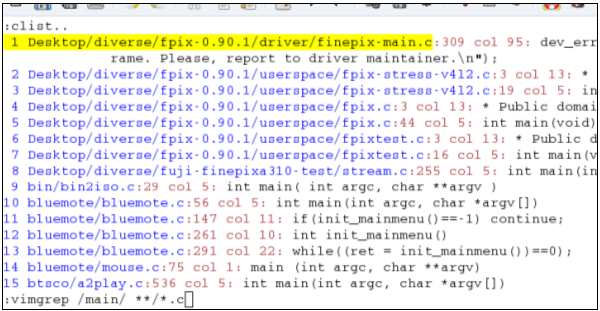
\includegraphics[scale=0.7]{./images/page66.png}
\end{center}
\marginpar{67}
\subsection{搜索帮助系统}
\label{subsec:search_the_help_system}

有时候需要从 Vim 中得到某些帮助信息, 此时用户可能并不确切地知道应该查找哪些信
息. 当然, 你可以在整个帮助系统中从头开始查找, 不过, Vim 的帮助系统包含众多的文
件, 以及数以千计的关键词.

为了解决这个问题, Vim 提供了一个专门的命令. 在前一节中, 用的是
\texttt{vimgrep}, 而对于 Vim 帮助系统, 则用的是下面这个命令:
\begin{vimcmdform}
\texttt{:helpgrep }\textit{pattern}\texttt{ [@LANG]}
\end{vimcmdform}
命令需要一个必填参数 --- 待搜索的模式 --- 还有一个是可选参数, 用于限定语
言, 先来看一个例子. 比如说用户需要一些关于自动补全的帮助信息, 但是不知道
从哪里开始查找. 因为用户只了解英文, 所以你希望帮助信息也是英文的. 完成这个搜索
的命令是:
\begin{vimcode}
:helpgrep completion@en
\end{vimcode}
命令所执行的操作是在所有的英文 (\texttt{en}) 文档中搜索单词 \texttt{completion}.
搜索完成后, 光标会跳转到第一个匹配, 剩下的匹配结果则添加到 quickfix 列表, 以便
稍后检索.

\begin{warning}
    如果用户想使用 location 列表, 而不是 quickfix 列表, 就用 \texttt{:lhelpgrep}
    替换掉 \texttt{:helpgrep}.
\end{warning}

实际上, 命令 \texttt{helpgrep} 并没有遍历所有的文档, 而是使用了 tag list 来搜索
模式. Tag list 并不会自动生成, 所以, 如果用户安装的插件带有自己的文档, 那就必须
使用下面的命令:
\begin{vimcode}
    :helptags /path/to/documentation
\end{vimcode}
把 \texttt{/path/to/documentation} 替换成新文档的安装位置, 但是为了能让 Vim 找
到文档, 新文档必须放在 Vim 选项 \texttt{runtimepath} 定义的几个目录的
\texttt{docs/} 子目录中 (参考 \texttt{:help 'runtimepath'}).
\marginpar{68}

\section{标记位置}
\label{sec:x_marks_the_spot}

有时, 当用户在编辑文件的某一行时, 需要跳到另一个地方查看一下. 之后, 可能很
难找到原来的那一行.

如果能在离开前作一下标记, 这样的话, 找到离开时的位置就方便多了.

为此, Vim 提供了一些工具用于完成这个功能. 这些工具可以分成两类:
\begin{itemize}
    \item 可见的标记
    \item 隐藏的标记
\end{itemize}

\subsection{可见的标记 --- 使用符号}
\label{subsec:visible_markers_using_signs}

在 Vim 中, 可以用一个可见的标记 --- 符号 --- 来标记一行. 一个符号指的是一
个标记, 它会显示在编辑器最靠左的列中.

\begin{warning}
    如果用户想改变显示符号的列的颜色, 可以使用下面这个命令:
    \begin{vimcode}
    :highlight SignColumn guibg=darkgrey
    \end{vimcode}
\end{warning}

根据所使用的 Vim 版本 (控制台或 GUI) 的不同, 符号或者是一些字符的组合 (比如
\texttt{>>}), 或者是一个图标. 为了使用符号, 需要作一些设置. 如果把设置信息写
在 \texttt{vimrc} 中, 就用不着每次都设置一遍.

第一件要做的事是定义你想用的符号. 定义符号的命令是:
\begin{vimcmdform}
\texttt{:sign define}\ \textit{name}\ \textit{arguments}
\end{vimcmdform}
\textit{arguments} 可以是下面几种之一:
\begin{itemize}
    \item \texttt{linehl}: 用于标记行的色彩组
    \item \texttt{text}: 该文本将作为符号, 显示在控制台 Vim 中 (比如
        \texttt{>>!!} 或 \texttt{++}). 每一个符号最多可以用两个字符.
    \item \texttt{texthl}: 用于标记符号文本的色彩组
    \item \texttt{icon}: 图标的完整路径, 该图标可用在 Gvim 的符号中. 图标应该
        足够小, 小到能够放到两个字符的空间中. 图标文件的格式可以是位图文件,
        不过最好是 \texttt{.xpm}.
\end{itemize}
\marginpar{69}
一个简单的例子是:
\begin{vimcode}
:sign define information text=!> linehl=Warning texthl=Error icon=/path/
to/information.xpm
\end{vimcode}
把符号定义好, 并且把定义的命令添加到 \texttt{vimrc} 后, 我们
已经准备好把该符号放到文件中的某个位置, 放置符号的命令是:
\begin{vimcode}
:exe ":sign place 123 line=" . line(.) ."name=information file=" .
expand("%:p") \end{vimcode}
用户可以把数字 \texttt{123} 替换成任意一个数字, 它将作为这个符号的 ID.

正如读者所看到的那样, 放置符号的命令写起来有点麻烦, 但可以把它映射到一
个键上.

命令的效果是把名字为 \texttt{information}, 且 ID 号为 \texttt{123} 的符号放置
到当前打开文件 (\verb'expand("%:p")') 的当前行 (\texttt{line(.)}). 映射的命令
是:
\begin{vimcode}
:map <F7> :exe ":sign place 123 line=" . line(".") ."name=infomation
file=" . expand("%:p")<CR>
\end{vimcode}
上面的命令把符号 \texttt{infomation} 映射到键 \key{F7}, 当你按下 \texttt{F7}
时, 符号就会被放置到当前行.
\begin{center}
    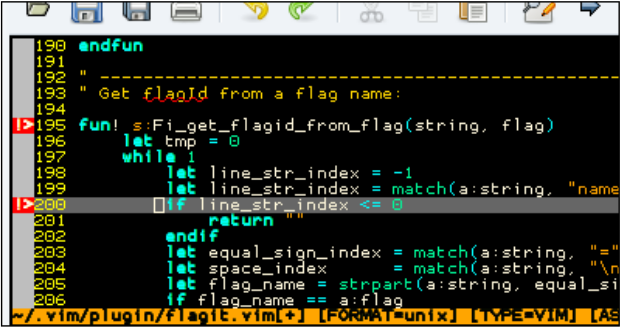
\includegraphics[scale=0.6]{./images/page69.png}
\end{center}
有时候, 用户想要移除符号, 用术语来讲, 叫作 ``unplace'' 一个符号:
\begin{vimcmdform}
\texttt{:sign unplace}\ \textit{ID}
\end{vimcmdform}
\marginpar{70}

命令中的 \textit{ID} 是放置符号时的 ID (在前面的例子中就是 \texttt{123}). 这个
命令会把所有的, 用该 ID 放置的符号移除. 用户可能只想把当前文件中的指定符号移
除, 这时候可以在命令的末尾加上另一个参数, 用来指定文件:
\begin{vimcmdform}
\texttt{:sign unplace}\ \textit{ID}\ \texttt{file=}\textit{name}
\end{vimcmdform}
或者用下面这个命令从当前缓冲区中移除符号:
\begin{vimcmdform}
\texttt{:sign unplace}\ \textit{ID}\ \texttt{buffer=}\textit{bufferno}
\end{vimcmdform}
命令中的 \textit{bufferno} 是当前缓冲区的编号 (可以通过命令 \texttt{:buffers}
查看).

如果只想移除当前行的符号, 用:
\begin{vimcode}
:sign unplace
\end{vimcode}
为了和放置符号的按键映射相对应, 把它映射到 \key{Ctrl+F7} 上:
\begin{vimcode}
:map <C-F7> :sign unplace<CR>
\end{vimcode}

\begin{warning}
    如果你在同一个文件中, 用同一个 ID 添加了多个符号, 那么上面的命令只会移除
    文件内最靠前的符号, 而非当前行的符号.
\end{warning}

既然本章讨论的是导航, 那么我们也要介绍一下如何跳转到一个符号. 这种跳转在 Vim 中
称为 符号跳转 (sign-jumping), 所使用的命令是:
\begin{vimcmdform}
\texttt{:sign jump}\ \textit{ID}\ \texttt{file=}\textit{file}
\end{vimcmdform}
命令中的 \textit{ID} 是你想要跳转到的符号 ID, \textit{file} 指定在哪个文件中
搜索该符号. 除了 \texttt{file=}\textit{file}, 还可以用 \texttt{buffer=}%
\textit{bufferno}.

同样, 如果在同一个文件/缓冲区内用同一个 ID 添加了多个符号, 那么命令只能跳转到
该 ID 在文件内的第一个符号.

\begin{warning}
    Paul Rouget 开发了一个 Vim 脚本, 通过它用户可以非常方便地使用符号. 脚本的
    下载地址是 \url{http://www.vim.org/scripts/script.php?script_id=1580}.
\end{warning}
\marginpar{71}

\subsection{隐藏的标记}
\label{subsec:hidden_markers_using_marks}

为了给当前行作标记, 用户可以使用标记 (mark). 它的使用方法非常简单, 总的来说,
它由两个在普通模式下使用的命令组成, 一个用于设置标记, 另一个用于跳转到标记.
除非打开标记列表, 否则用户无法判断某一行是否含有标记.

首先来看一下如何标记当前行. 为了标记当前行, 只需要在普通模式下按下
\texttt{m}, 后面再紧跟着某个字符, 这个字符可以是 \texttt{0}-\texttt{9},
\texttt{a}-\texttt{z},或 \texttt{A}-\texttt{Z} 中的一个. 例如, 如果用户执行
了 \texttt{ma}, 那就是说用名字为 \texttt{a} 的标记来标记当前行. 然后, 如果用户
想要跳转到标记 \texttt{a} 所在的行, 只需要按下 \texttt{'a} (单引号 + 标记名),
光标就会马上跳转到该行的开始 (如果该行是缩进过的, 那就跳转到该行的第一个非空白字
符).

有时候, 光是跳转到一行的开始可能还不够, 如果能直接跳转到添加标记时光标所在的具
体位置可能会更好一点. 为了达到这个目的, 需要把跳转命令中的单引号改成反单引号
(\texttt{`}), 于是, 跳转到标记 \texttt{a} 的命令就变成了 \texttt{`a}.

不同的标记名含有不同的意义, 它们的使用范围如下所示:
\begin{center}
    \begin{tabular}{lp{40em}}
    \hline
    标记        & 用法 \\
    \hline
    \texttt{0}-\texttt{9} & 这个标记集来源于文件 \texttt{.viminfo}, 通常保留
    给 Vim 内部使用 (比如, 标记 \texttt{0} 表示文件最后一次退出时, 光标所在的
    位置. 然而, 用户可以利用这些标记来实现 ``打开最近使用过的文件''. \\
    \texttt{a}-\texttt{z} & 这些标记只在当前文件内有效, 当文件关闭时删除这些
    标记. 如果用户此时是在当前文件的缓冲区内, 那么只能通过这些小写字母标记在
    文件内跳转. \\
    \texttt{A}-\texttt{Z} & 这些标记可以跨越文件使用. 即使没有打开目的标记所在
    的文件, 也可以直接跳转到标记所在的位置. 如果 \texttt{.viminfo} 文件是可用
    的, 那么这些标记就会被保存下来, 直到下一次对文件进行编辑. \\
    \hline
\end{tabular}
\end{center}

用户可以通过下面这个命令来获取完整的, 正在使用的标记列表:
\begin{vimcode}
:marks
\end{vimcode}
命令显示了每个标记所在的文件与行号. 为了删除一个或多个标记, 执行:
\begin{vimcmdform}
\texttt{:delmarks}\ \textit{markid markid...markid}
\end{vimcmdform}
具体的使用例子有:
\begin{vimcode}
:delmarks a b c
:delmarks a-c
:delmarks a f-i 1-4
\end{vimcode}
\marginpar{72}
如果用户想要删除当前缓冲区内的所有标记, 执行:
\begin{vimcode}
:delmarks!
\end{vimcode}

当使用 Vim 时, 它会自动设置其他类型的标记. 其他类型的标记包括但不限于: 最后
一次退出插入模式时光标所在的位置; 可视模式下被选中的文本的开始与结束; 最后一
次被修改的地方.

关于如何使用标记, 以及其他类型标记的更多信息, 参考 \texttt{:help mark-motions}.

\section{小结}
\label{sec:better_navigation_summary}

这一章介绍了在文件与缓冲区内快速导航的方法.

首先介绍了如何根据文件的上下文结构, 在文件内部快速导航. 除此之外, 还讨论了
如何在冗长并且折叠过的行中移动光标.

然后介绍了如何在 Vim 的帮助系统中导航, 还学习到了如何通过简单的按键绑定,
使得导航更加直观, 便于记忆.

既然已经知道了如何在文件内导航, 还要知道如何在多个文件与多个缓冲区之间导航.
再接下来的小节我们学习了如何快速地在缓冲区之间导航, 以及如何通过两次击键, 来
打开被另一个文件所引用的文件.

导航的方式有许多种, 在接下来的小节我们学习到利用搜索, 不仅可以在打开的文件内
导航, 甚至包括磁盘上的文件. 还学习了如何在 Vim 的帮助系统搜索某个主题的相
关帮助信息.

最后, 我们学习了如何通过符号与标记在文件间跳转, 以及使用 Vim 时, 它会如何
自动地帮助用户添加标记.

我们已经学习到了如何在 Vim 中迅速地导航, 可以继续阅读下一章节. 下一章
将会用到更多的 Vim 内置功能 来提高工作效率.

% vim: ts=4 sts=4 sw=4 et tw=80
\chapter{助推器}
\label{chap:production_boosters}

\marginpar{73}
在这一章将会看到, 即使是一些小小的改动, 也可以极大地促进 Vim 的工作效率.
有些技巧是由 Vim 的特性提供的, 另外一些则需要用户自已编写一些脚本.

无论你把 Vim 当成一个修改配置文件的小工具, 还是把它用作某个大型开发项目的主要
编辑器, 你都可以发现本章介绍的方法可以极大地提高 Vim 的使用效率.

这一章讨论的主题包括:
\begin{itemize}
    \item 使用模版文件的模版
    \item 使用缩写的模版
    \item 使用已知单词与 tag list 的自动补全
    \item 使用 omnicompletion 的自动补全
    \item 宏与宏录制
    \item 使用会话
    \item 使用会话的项目管理
    \item 寄存器与撤消分支
    \item 折叠
    \item 使用 \texttt{vimdiff} 分析差异
    \item 使用 \texttt{netrw} 随时随地地打开文件
\end{itemize}

阅读完这一章之后, 用户使用 Vim 的工作效率应该可以提高好几个百分点.
\marginpar{74}

\section{使用模版}
\label{sec:using_templates}

无论编辑的是哪一种类型的文件, 当打开一个新文件时, 总有一些基础性的工作需要完成.
手动完成这些基础工作是一件非常乏味的事件, 更讨厌的是每次打开一个新文件时, 都
要重新再做一遍. 所以说干嘛要花这么多的时间, 来做一件使用模版就可以完成的事情?

在接下来的两节, 将会看到一些不同类型的模版. 其中一些模版特定于文件类型, 另
外一些则会使用用户的输入来触发小内容模版 (比如, 程序员经常用到的代码片断).

\subsection{使用模版文件}
\label{subsec:using_template_files}

每次打开一个新文件时, 用户做的第一件事经常是输入某些头部信息, 当然, 所要输入的
信息取决于文件的类型. 比较常见的例子包括:
\begin{itemize}
    \item 在新的 HTML 文件中添加基本结构 (\texttt{<html>}, \texttt{<head>},
        \texttt{<body>}).
    \item 在所有的 C 文件添加头部信息, 在文件 \texttt{main.c} 中添加
        \texttt{main()} 函数.
    \item 在 Java 文件中添加主类.
\end{itemize}
除了这些, 读者应该还能想到其他一些例子.

那么, 怎么才能创建一个模版文件? 不妨用 HTML 文件作为例子来进行讲解.
这种文件的结构是静态的, 因此非常适合用模版来处理. HTML 模版的内容是:
\begin{vimcode}
<html>
    <head>
        <title></title>
            <meta name="generator" content="Vim" />
            <meta name="author" content="Kim Schulz" />
    </head>
    <body>
        <p>Content goes here...</p>
    </body>
</html>
\end{vimcode}
在 \texttt{VIMHOME} 目录下创建一个新目录 \texttt{templates/}, 并把上面的
模版文件保存到这个目录中, 假设把模版文件命令为 \texttt{html.tpl}.
\marginpar{75}
现在, 第一个模版已经准备就绪, 不过, 创建一个新的 HTML 文件时, 需要加载
模版文件, 为了完成加载, 把下面这行命令添加到 \texttt{vimrc} 中:
\begin{vimcode}
:autocmd BufNewFile *.html 0r $VIMHOME/templates/html.tpl
\end{vimcode}
这个命令可以确保在新建一个 \texttt{*.html} 文件时, 模版文件的内容会自动加
载到新文件中. 于是, 在开始编辑新文件前, 文件中就已经包含了模版的内容.

本来这样做没什么问题, 但是当添加的模版文件越来越多时, 用户可能会越来越讨厌每
次都要往 \texttt{vimrc} 中添加一行加载命令. 所以, 把加载模版的命令写得
更灵活一点:
\begin{vimcode}
:autocmd BufNewFile * silent! 0r $VIMHOME/templates/%:e.tpl
\end{vimcode}
命令的功能是: 无论何时打开一个新文件, Vim 就在模版目录中搜索以文件扩展名命名
的模版. 比如, 创建一个 \texttt{index.html} 文件时, Vim 就在
\texttt{\$VIMHOME/templates/} 中搜索名为 \texttt{html.tpl} 的模版文件.

如果没有找到指定的模版, Vim 就创建一个空文件.

再把模版写得更完善一点: 添加对占位符 (占位符指的是将要添加文本的地方) 的
支持. 一个占位符看起来可以非常得与众不同, 这取决于用户, 我通常把它们显示成类似
于 \texttt{<+KERWORD+>} 的形式. 如果在前面的 HTML 模版中添加上占位符,
模版的内容就变成了:
\begin{vimcode}
<html>
    <head>
        <title><+TITLE+></title>
            <meta name="generator" content="<+GENERATOR+>" />
            <meta name="author" content="<+AUTHOR+>" />
    </head>
    <body>
        <p><+CONTENT+></p>
    </body>
</html>
\end{vimcode}

现在, 已经准备好了占位符, 接下来的工作就是在占位符之间跳转. 为了让跳转更加
方便, 把跳转命令添加到 \texttt{vimrc} 中. 用户可能想要把组合键 \key{Ctrl+j}
映射到跳转命令, 因为这样做的话便于在插入模式下使用, 组合键中 \texttt{j} (意
指 jump) 也更容易记忆. 映射组合键的命令是:
\begin{vimcode}
nnoremap <c-j> /<+.\{-1,}+><cr>c/+>/e<cr>
inoremap <c-j> <ESC>/<+.\{-1,}+><cr>c/+>/e<cr>
\end{vimcode}
\marginpar{76}
现在, 只需要按下组合键 \key{Ctrl+j}, 你就可以方便地跳转到文件中的下一个占位符,
输入文本, 然后再跳转到下一个占位符.

通过在占位符中添加关键字, 就可以提醒用户应该在占位符中输入什么样的内容.

\begin{warning}
可以通过命令 \texttt{match} 高亮显示占位符, 具体的设置命令是:
\verb'match Todo /<+.\++>/', 把这行命令添加到 \texttt{vimrc} 中 (可以把命令中的
\texttt{Todo} 替换成任意一种你喜欢的色彩组.
\end{warning}

\subsection{把缩写作为模版}
\label{subsec:abbreviations_as_templates}

上一小节介绍了如何为不同类型的文件制作模版, 这一节介绍如何为文件内容制作模版.

第 \ref{chap:personalizing_vim} 章简单地介绍了如何通过缩写来减少击键的
次数, 现在把缩写应用到模版中. 回忆一下下面这个命令的作用:
\begin{vimcode}
:iabbrev match replace-string
\end{vimcode}
我们只想让上面的命令工作在插入模式, 这是因为模式模版本来就应该工作在插入模式下.
对于 C 文件来说, 一个常见的例子是:
\begin{vimcode}
:iabbrev <buffer> for( for (x=0;x<var;x++){<cr><cr>}
\end{vimcode}
无论在什么时候输入文本 \texttt{for(}, Vim 都会自动插入一段 \texttt{for} 循
环. \texttt{(} 可以防止手工输入的 \texttt{for} 循环被自动转换. 插入的内容看起
来就像:
\begin{vimcode}
for (x=0;x<var;x++){

}
\end{vimcode}

\begin{warning}
    缩写词左边的 \texttt{<buffer>} 把命令的作用范围限制在当前缓冲区内.
\end{warning}

正如你所看到的那样, 生成的代码模版是静态的. 为了让模版更灵活一点, 把前面一节介
绍的占位符应用进来.
\marginpar{77}
在这种情景下使用的占位符更像是一个跳转点, 因此把它们简化成 \texttt{<+++>}.
除此之外, 在插入模式模版之后, 需要在光标的下一个位置上放置一个占位符, 对于
前面的例子来说, 光标的下一个位置应该是左括号的右边.

为了实现这个目标, 引入 \texttt{!cursor!} 占位符, 命令的内容是:
\begin{vimcode}
iabbrev for( for(!cursor!;<+++>;<+++>){<cr><+++><cr>}<Esc>
    :call search('!cursor!','b')<cr>cf!:
\end{vimcode}
(上面的命令都在同一行上)

现在, 无论何时输入 \texttt{for(}, Vim 都会自动插入一段 \texttt{for} 循环, 然后
把光标移动到占位符 \texttt{!cursor!} (当光标移过来时, 占位符上原来的内容会自动
被移除). 接下来, 用户就可以方便地填写 \texttt{for} 循环的参数, 并用 \key{Ctrl+j}
跳转到下一个参数的位置.

也许读者已经知道, 许多编程语言都有相同的主要结构 (比如 \texttt{for} 循环), 但是
它们之间的差异导致了无法使用同一个模式模版. 再回过头来看一下手上已有的东西,
看看是否可以让它们识别文件类型.

前面的一节介绍了如何根据文件的扩展名来加载相应的模版文件, 具体的命令
是:
\begin{vimcode}
:autocmd BufNewFile * silent! 0r $VIMHOME/templates/%:e.tpl
\end{vimcode}
对这个命令进行修改, 使得 Vim 可以根据文件的类型, 为模式模版自动加
载适当的缩写.

为了能让命令更聪明一点, 把命令的功能用函数来实现. 函数的代码是:
\begin{vimcode}
function! LoadTemplate(extension)
    silent! :execute '0r $VIMHOME/templates/'. a:extension. '.tpl'
    silent! execute 'source $VIMHOME/templates/'.a:extension.'.patterns.tpl'
endfunction
\end{vimcode}
为了调用函数, 把 \texttt{autocmd} 修改成:
\begin{vimcode}
:autocmd BufNewFile * silent! call LoadTemplate('%:e')
\end{vimcode}
函数 \texttt{LoadTemplate} 在 \texttt{\$VIMHOME} 的 \texttt{templates} 子目录
下搜索两个文件: \texttt{EXTENSION.tpl} 与 \texttt{EXTENSION.patterns.tpl},
其中 \texttt{EXTENSION} 表示当前打开着的文件的扩展名.
\marginpar{78}
第 1 个文件包含了特定文件类型的模版, 而第 2 个文件则包含了特定文件类型的缩写
命令. 如果没有找到对应的文件, 那么命令 \texttt{silent!} 就会抑制错误信息的输
出, 什么也不会显示出来.

现在, 模版文件中该包含什么样的内容完全由用户来决定.

\begin{warning}
    已经有人为 Vim 编写了大量的模版系统脚本, 其中大部分都是以本章介绍的概念为基础,
    但是增加了许多额外的功能. 除了这里介绍的之外, 如何用户还想要更多的模版选项,
    笔者推荐你看一下由 Gergely Kontra 编写的 mu-template, 可以到下面这
    个网址下载: \url{http://www.vim.org/scripts/script.php?script_id=222}.
\end{warning}

\subsection{snipMate 脚本}
\label{subsec:snippets_with_the_snipmate_script}

虽然已经有大量的模版系统脚本可供使用, 而且它们中的大部分都是以本章介绍的概念
为基础, 但是有时候对于特定的文件格式, Vim 还是没有提供足够的支持. 对于这些情况,
用户可以使用 snippet 脚本. Snippet 和用在模版中的缩写有点类似, 但是要更高级一
点.

如果读者想在 Vim 中使用 snippet, 笔者推荐 snipMate 脚本, 下载地址是
\url{http://www.vim.org/scripts/script.php?script_id=2540}.

snipMate 可以让用户在不需要了解 Vim 脚本的前提下, 为自己的文件格式定义高级的
snippet.

假设用户想为 \texttt{for} 循环创建一个 snippet (在前面的一节里用的是
\texttt{iabbrev}),  那就这样做:
\begin{vimcode}
snippet for
    for (${1:i} = 0; $1 < ${2:count}; $1${3:++}) {
        ${4:/* code */}
    }
\end{vimcode}
把上面这段文本写到一个文件中, 再把这个文件放到 \texttt{\$VIMHOME/snippets} 目
录下, 把文件命名为 \textit{filetype}\texttt{.snippet} (\textit{filetype}
表示文件类型,
比如 C 代码就写成 \texttt{c.snippet}, PHP 代码就写成 \texttt{php.snippet}).
\marginpar{79}
脚本的第一行表示开始一个新的 snippet, 当输入 \texttt{for} 并且后面再紧跟着一个
\key{Tab} 键时, 执行 snippet 脚本.

再接下来的一行是最神奇的, 脚本实际生成的代码看起来就像:
% FIXME
\begin{vimcode}
    for (i = 0; I < count; i++) {
        /* code */
    }
\end{vimcode}

snippet 被插入之后, 它把光标放在了第 1 个 \texttt{i} 的位置, 并切换到插入
模式, 可以轻易地把 \texttt{i} 换成另一个变量. 现在, 最神奇的事情发生了,
% FIXME
第 1 个 \texttt{i} 被换掉之后, 第 2 个 \texttt{i} (后面带有 \texttt{++}
的那个) 也会被自动更新成新变量. 修改了 \texttt{i} 之后 (如果需要的话), 按下
\key{Tab} 键, 光标就会跳转到 \texttt{count}, 并再次切换到插入模式. 现在你可以
以同样的步骤修改 \texttt{count} 并按下 \key{Tab} 键, 之后, 光标跳转到
\texttt{++}, 再按下 \key{Tab} 跳到 \texttt{/* code */}, 你可以在这里写下其他代
码.

在 snippet 的不同变量之间跳转, 简直不能再简单了.

snipMate 系统通过查找由 \texttt{\$\{NUMBER:INITIAL\_VALUE\}} 创建的特殊标记进行
工作. 标记中的 \texttt{NUMBER} 指出了按下 \key{Tab} 时, 将要跳转到的序列.
如果 \texttt{NUMBER} 是 1, 那么光标会首先处在这个位置上, 如果 \texttt{NUMBER}
是 3, 那么它就是按下两次 \key{Tab} 后光标所在的位置, 以此类推.
\texttt{INITIAL\_VALUE} 是在修改 snippet 之前, 首先插入到 snippet 中的文本.
比如 \texttt{\$\{1:i\}} 把 \texttt{i} 作为文本插入到 snippet 中, 并首先把光标
放在此处.

如果需要在多个地方使用同一个变量, 可以通过 \texttt{\$NUMBER} 来引用. 比如说,
想要让 \texttt{i} 出现在多个地方, 那就在需要出现 \texttt{i} 的地方写上
\texttt{\$1} 即可. 写上 \texttt{\$1} 所有地方在开始时都会显示成 \texttt{i},
当改变 \texttt{i} 时, 其他地方的 \texttt{i} 也会自动更新.

这里介绍的只是创建 snippet 的基础知识, 不过一旦在系统中安装了 snipMate,
就可以通过 Vim 的帮助系统学习到更多的高级知识.

还可以在 snipMate 中找到更多的惊喜. 用户会发现, snipMate 已经为许多常见
的文件格式准备好了 snippet 脚本, 包括 \texttt{.c}, \texttt{.php},
\texttt{.perl}, \texttt{.java}, \texttt{.html}, \texttt{.tex}, 甚至还包括 Vim
脚本.
\marginpar{80}

\begin{warning}
    关于下载与如何使用 snipMate 脚本, 用户可以访问
    \url{http://www.vim.org/scripts/script.php?script_id=2540}.
\end{warning}

\section{Tag List}
\label{sec:using_tag_list}

Tag list 就像是程序员的字典. Tag list 实际上是一个包含了所有种类的关键词的文件,
这些关键词可以用来识别程序的各个要素, 包括函数名, 变量名, 类的方法, 具体的要素
依赖于编程语言. Tag list 文件并非由 Vim 生成, 而是 tag list 生成程序. Tag list
生成程序有很多种, 比较常见的有:
\begin{itemize}
    \item Exuberant Ctags: 用于 C, C++, Java, Perl, Python, Vim, Ruby (以及其
        他 25 种语言)
    \item Vtags: 用于 Verilog 文件
    \item Jtags: 用于 Java 文件
    \item Hdrtags: 用于 C/C++, Asm, Lex/Yacc, LaTeX, Vim, Maple
    \item Ptags: 用于 Perl 文件
\end{itemize}

因为 Exuberant Ctags (简称 Ctags) 使用得最为广泛, 支持的语言也是最多的, 因此
在下面的例子里我们用它生成 tag list.

以一个小项目进行讲解, 这个项目包含了 3 个 C 文件:
\begin{itemize}
    \item \texttt{main.c}: 包含 \texttt{main} 函数的文件
    \item \texttt{myfunctions.c}: 包含了程序中用到的各个函数
    \item \texttt{myfunctions.h}: \texttt{myfunctions.c} 中的函数的头文件
\end{itemize}
假设代码已经写完, 现在为这些代码文件生成一个 tag list 文件.

在存放源代码文件的目录下执行命令:
\begin{vimcode}
ctags *.c *.h
\end{vimcode}
命令执行完毕后, 会在当前目录下创建一个新文件, 文件名是 \texttt{tags}.
这个文件就是 tag list 文件, 它包含了源代码中所有函数与变量的信息.
\marginpar{81}
\begin{warning}
    \texttt{ctags} 命令提供了大量的参数, 用于指定编程语言, 更多的信息可以通过
    \texttt{ctags --help} 来查看.
\end{warning}
启动 Vim 后, 必须告诉它去使用 \texttt{tags} 文件, 这可以通过设置选项
\texttt{tags} 来完成:
\begin{vimcode}
:set tags=/path/to/tags
\end{vimcode}
现在, Vim 已经知道了 \texttt{tags} 文件的存在, 接下来就可以在 Vim 使用它.

\texttt{main.c} 调用了 \texttt{myfunctions.c} 中定义的函数. 假设用户
知道有一个函数叫作 \texttt{calcValue}, 但却不知道该函数接收什么样的参数, 比较
好的做法是看一下函数是如何定义的, 这时候就可以使用 \texttt{tags} 文件提供的功
能. 假设用户已经在源代码文件中写下了:
\begin{vimcode}
myvalue = calcValue(
\end{vimcode}
为了查看函数 \texttt{calcValue} 的定义, 把光标移动到函数名上, 按下组合键
\key{Ctrl+]}, 此时会出现下面两种情况中的一种:
\begin{itemize}
    \item 只找到一个匹配, 于是光标会直接跳转到定义函数的地方
    \item 找到多个匹配, 于是 Vim 把这些匹配以列表的形式显示出来
\end{itemize}
在第 2 种情况下, 用户可以选择跳转到哪一个匹配. 如果用户使用的编程语言支持重载,
就会出现这种情况: 同一个函数有多个版本.

函数看完之后, 用户需要回到之前离开的地方, 继续往下工作. 按下组合键
\key{Ctrl+t} 就可以跳转到上一次离开的地方.

\begin{warning}
    如果用的是 Gvim, 还可以通过鼠标来跳转到关键词的定义: 按住 \key{Ctrl} 键
    的同时, 按下鼠标左键.
\end{warning}
用户可以把在 tag 间的跳转当成栈操作. 当跳转到一个关键词时, 相当于把关键词的 tag
压栈, 从 tag 返回时, 相当于把栈顶的 tag 弹出栈.
\marginpar{82}
使用下面这个命令查看当前的栈状态:
\begin{vimcode}
:tags
\end{vimcode}
\begin{center}
    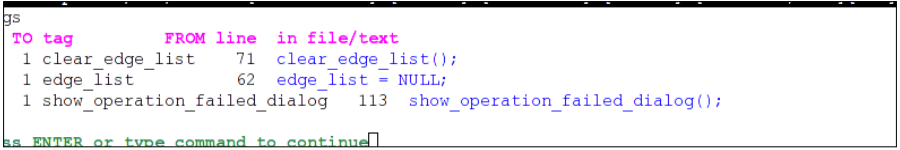
\includegraphics[scale=0.5]{./images/page82.png}
\end{center}
上图中以 \texttt{>} 开始的行是当前所在的 tag. 除了组合键 \key{Ctrl+]}
与 \key{Ctrl+t}, 还可以用下面这两个命令完成同样的功能:
\begin{itemize}
    \item \texttt{:tag}: 跳转到这个 tag
    \item \texttt{:pop}: 回到上一个 tag
\end{itemize}

如果匹配的 tag 比较多, 要是能把这些 tag 以列表的形式罗列出来可能会比较方便.
为了得到这个列表, 可以用下面两个命令中的任意一个:
\begin{itemize}
    \item \texttt{:tselect}
    \item \texttt{:ptselect}
\end{itemize}
第 1 个命令列出所有匹配的 tag, 为了选择其中一个, 需要输入 tag 所在行的行首的
数字.

第 2 个命令完成同样的工作, 但是它会在预览窗口中显示列表. 如果用户选错了 tag,
或者是想查看列表中的下一个 tag, 可以用下面的命令在 tag 间移动:
\begin{itemize}
    \item \texttt{:tnext}: 移动到列表中的下一个 tag
    \item \texttt{:tprev}: 移动到列表中的前一个 tag
\end{itemize}

用户可能还没有从前面的例子中体会到 tag list 的强大之外, 想像一下, 假设项目中的
文件不只 3 个, 而是散布在数百个目录中的上千个文件, 这时候, 用户肯定没办法记住
每个函数所在的位置, 这时候就非常需要一个强大的索引工具, 就像 tag list.
\marginpar{83}
\subsection{更便捷的 taglist 导航}
\label{subsec:easier_taglist_navigation}

在大多数的非英文键盘布局中, 按键 \texttt{]} 无法直接使用, 必须通过其他的组合
键 --- 比如 \key{Ctrl+Alt+G+r+9} --- 完成 \key{Ctrl+]} 的功能. 在这种情况下,
把命令映射到直接可用的按键上会更方便一点, 对此, 笔者使用了下面的映射:
\begin{vimcode}
:nmap <buffer> <F7> <C-]>
:nmap <buffer> <C-F7> <C-T>
:nmap <buffer> <A-F7> :ptselect<cr>
:nmap <buffer> <F8> :tnext<cr>
:nmap <buffer> <C-F8> :tprev<cr>
\end{vimcode}
现在, 用户可以用 \key{F7} 与 \key{Ctrl+F7} 在 tag 间跳转, 用 \key{Alt+F7}
获取 tag 列表, 用 \key{F8} 与 \key{Ctrl+F8} 遍历 tag.

\subsection{taglist 的其他用法}
\label{subsec:other_usages_of_taglists}

Taglist 不仅可以用来查找函数与变量的定义, 还可以用来查找其他信息. 笔者在这里只
是简单地提一下 taglist 在 Vim 中的其他应用:
\begin{itemize}
    \item \texttt{lookupfile.vim}: 由 Hari Krishna Dara 开发, 该脚本使用 tag
        list 在一个预处理过的项目中查找指定的文件, 脚本的最新版见
        \url{http://www.vim.org/scripts/script.php?script_id=1581}.
    \item \texttt{taglist.vim}: 由 Yegappan Lakshmanan 开发的插件, 在程序员中
        非常流行. 它是一个完整的源代码浏览工具, 在一个分割的窗口中显示函数,
        关键词, 变量, 定义的概览. 插件的下载地址是
        \url{http://www.vim.org/scripts/script.php?script_id=273}.
    \item \texttt{ctags.vim}: 由 Gary Johnson 与 Alexey Marinichev 开发.
        脚本可以在状态条或窗口标题栏中显示光标所在位置的函数的名字. 脚本使用
        Exuberant Ctags 为当前打开的文件自动生成 tag 文件. 脚本的下载地址是
        \url{http://www.vim.org/scripts/script.php?script_id=610}.
    \item \texttt{autoproto.vim}: Jochen Baier 专门为 C 程序员开发的脚本. 当
        程序员输入函数名与第一个左括号后, 脚本在预览窗口中显示该函数的原型.
        脚本的下载地址是
        \url{http://www.vim.org/scripts/script.php?script_id=1553}.
\end{itemize}
\marginpar{84}
\begin{warning}
    关于 tag 的更多信息与使用方法, 可以查阅 Vim 的帮助系统 \texttt{:help tags}.
\end{warning}

\section{使用自动补全}
\label{sec:using_autocompletion}

作为一个遵循 Vim 哲学的用户, 总是希望用最少的击键来完成一件事, 因为额外的击键
意味着额外的时间.

所以说, 如果 Vim 可以猜出用户正想打的单词, 并且可以自动补全, 那又何必每次
都从头输到尾呢?

在 Vim 中有多种办法来自动补全单词, 其中一些只能补全用户曾经在某个打开的缓冲区
中输过的单词, 还有一些牵涉到了对当前正在使用的代码的分析 --- 不仅仅是当前打开
文件, 还包括整个源代码树.

接下来的小节讨论使用自动补全的三种方法:
\begin{itemize}
    \item 已知单词的自动补全
    \item 基于字典文件的补全
    \item 识别上下文的自动补全
\end{itemize}
除此之外, 还会介绍一些使用技巧, 通过按键绑定来更方便地使用自动补全.

\subsection{已知单词的自动补全}
\label{subsec:autocompletion_with_known_words}

这一节将会看到自动补全的最简单的用法 --- 为已知单词进行补全.

无论用户在写什么内容, 都会出现输入重复单词的情况. 在 Vim 中, 用户可以在输入
完单词的头两个字母后, 按下组合键 \key{Ctrl+n}.
\marginpar{85}

假设用户想要在 Vim 中输入 ``I have beautiful flowers in my flower garden''.

在刚开始时, 文件中没有任何其他的内容, 因此用户不得不一个字母一个字母地写下
文本的开始部分, 直到 ``I have beautiful flowers in my f''.

用户接下来会输入单词 ``flower'', 但是, 由于在前面已经输入了 ``flowers'',
当输入 ``f'' 后, 按下 \key{Ctrl+n}, Vim 就会把 ``f'' 自动扩展为 ``flowers'',
只要把多余的 ``s'' 删掉即可. 和输入整个单词相比, 这要快很多.

随着文本的增多, 读者会发现越来越多的单词可以自动补全.

组合键 \key{Ctrl+n} 所做的工作是向前搜索匹配的单词. 如果用户知道自己刚刚才输入
过同样的单词, 那么用 \key{Ctrl+p} 会更快一点, 因为这个组合键是向后搜索匹配.
一般来说, 除非文件非常大, 或者可能的匹配非常多, 否则 \key{Ctrl+n} 与
\key{Ctrl+p} 对用户来说并没有太大的区别.

\subsection{使用字典的自动补全}
\label{subsec:autocompletion_using_dictionary_lookup}

一个比较好的使用技巧是把用户所使用的语言的全部单词, 都搜集到一个巨大的字典
文件中, 然后再把这个文件作为字典加载到 Vim 中 (在因特网上很容易搜索到这种文件).
为了把文件作为字典载入到 Vim 中, 执行下面的命令:
\begin{vimcode}
:set dictionary+=/path/to/dictionary/file/with/words
\end{vimcode}
现在, Vim 已经事先知晓了大量的单词, 用户可以利用这些单词进行自动补全. 不过,
有一些地方会不一样. 因为补全时被搜索的单词并非在某个打开的缓冲区中, 而是
在选项 \texttt{dictionary} 所配置的字典文件中, 所以需要用另一个快捷键:
\key{Ctrl+x+k}.
\marginpar{86}
按下 \key{Ctrl+x} 后, 会进入补全模式, 再接着按下 \key{Ctrl+k}, 就可以在字典中
查询关键词 (\key{k} 指是的是 keyword).
\begin{center}
    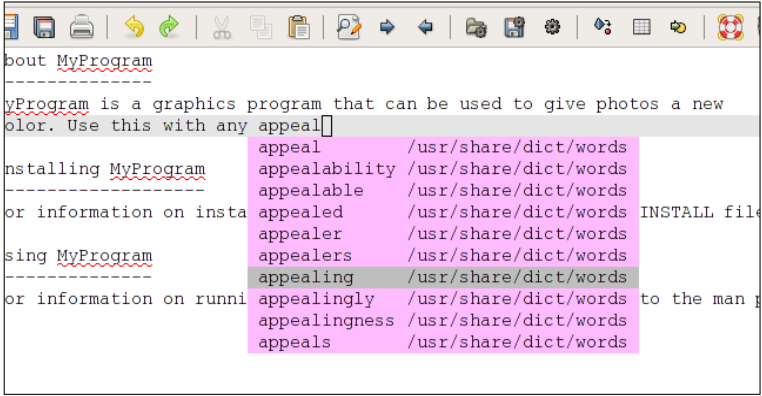
\includegraphics[scale=0.6]{./images/page86.png}
\end{center}

还有其他几种补全类型, 包括:

\key{Ctrl+x} 后跟:
\begin{itemize}
    \item \key{Ctrl+l}: 补全一整行文本
    \item \key{Ctrl+n}: 从当前缓冲区中补全单词
    \item \key{Ctrl+k}: 从字典中补全单词
    \item \key{Ctrl+t}: 从同义词典中补全单词 (见 \texttt{:help 'thesaurus'})
    \item \key{Ctrl+i}: 从当前文件与被包含的文件中补全单词
    \item \key{S}: 拼写建议 (仅 Vim 7.0 以上的版本支持)
\end{itemize}

其他的将会在下节介绍.

\subsection{omnicompletion}
\label{subsec:omnicompletion}

哪些内容应该自动补全, 哪些内容不应该自动补全 --- 对此我们都有完美的解决办法.
但是对于 Vim 来说, 在 7.0 版出现之前, 用户对补全并没有绝对的控制权.

Vim 7.0 引入了一种全新的补全技术 --- omnicompletion. 它使得用户可以精确地定义
补全功能应该如何工作. 实际上, 用户需要自己来编写补全函数 (除非已经有人把函数
写好了).
\marginpar{87}
和前一节介绍的一样, 激活补全的方法是先输入几个字母, 按下 \key{Ctrl+x} 进入到
补全模式, 再紧接着按下 \key{Ctrl+o} 使用 omnicompletion.

为了添加用户自定义的补全函数, 执行:
\begin{vimcode}
:set omnifunc=MyCompleteFunction
\end{vimcode}
现在, 用户只需要定义函数 \texttt{MyCompleteFunction}, 这个函数用于完成补全操作.
上面的命令只在当前活动缓冲区内才有效, 如果希望每个缓冲区都可以使用该补全函数,
那么就要对每个缓冲区执行这个设置命令.
\begin{warning}
    \texttt{omnifunc} 的设置通常在文件类型插件内完成, 这样的话, 补全函数就可以绑
    定到特定的文件类型上.
\end{warning}

现在来看一个补全函数的例子. 假设用户有一个通讯录文件, 文件的内容是人名及其邮件
地址, 就像:
\begin{vimcode}
Kim Schulz|kim@schulz.dk
John Doe|john.doe@somedomain.com
Jane Dame|jd@somedomain2.com
Johannes Burg|jobu@somedomain3.net
Kimberly B. Schwartz|kbs@somedomain.com
\end{vimcode}

用户想在写完一个人名后, 通过补全插入对应的邮件地址, 完成这个功能的函数是:
\begin{vimcode}
function! CompleteEmails(findstart, base)
	  if a:findstart
	    " locate the start of the word
	    let line = getline('.')
	    let start = col('.') - 1
	    while start > 0 && line[start - 1] =~ '\a'
	      let start -= 1
	    endwhile
	    return start
	  else
	    " find contact names matching with "a:base"
	    let res = []
		 " we read contactlist file and sort the result
	    for m in sort(readfile('/home/kim/.vim/contacts.txt'))
	      if m =~ '^' . a:base
				let contactinfo = split(m, '|')
\end{vimcode}
\marginpar{88}
\begin{vimcode}
		      " show names in list, but insert email address
		      call add(res, {'word': contactinfo[1],
                     \ 'abbr': contactinfo[0].' <'.contactinfo[1].'>',
                 \ 'icase': 1} )
	      endif
	    endfor
	    return res
	  endif
	endfunction
\end{vimcode}

函数接收两个参数 --- 所有的 omnicompletion 函数都是如此. Vim 第一次调用函数时,
把第 1 个参数 \texttt{findstart} 设置为 1 (\texttt{base} 为空). 这样的参数状态
表示这是第一次调用, 函数应该搜索用户当前所写的单词的开始.

然后, Vim 再次调用函数, 这次调用把 \texttt{findstart} 设置为 0, 把 \texttt{base}
设置成开始补全的单词. 这一次, 函数会打开通讯录文件, 以行为单位, 把文件读到
一个列表中, 对列表排序, 然后遍历列表.

每一行的内容按照 \texttt{|} 分割, 如果某个单词, 是以用于补全的单词的字母作为开
始, 那就把这个单词添加到结果列表中, 这个结果列表最后会作为函数的返回值返回.
函数可以修改弹出内容的外观, 和它所匹配的内容, 这两个功能无法通过添加电子邮件
地址来完成, 而是要通过构建一个字典 (见 \texttt{:help Dictionary}), 在构建字典
时会接触到一些特定的关键词. 在这个案例中使用下列三个关键词:
\begin{itemize}
    \item Word: 应该插入的真正的单词
    \item Abbr: 在弹出列表中使用的单词, 而非直接使用 word
    \item Icase: 如果其值非零, 则匹配是区分大小写的
\end{itemize}

其他的关键词及其意义可以在 Vim 的帮助系统中找到:
\begin{vimcode}
:help 'omnifunc'
\end{vimcode}

现在 Vim 已经有了一个单词列表用于补全, 在这个案例中则是一些像下面这样的行:
\begin{vimcode}
"Kim Schulz <kim@schulz.dk>"
\end{vimcode}
无论何时写下一些字母,比如 \texttt{ki}, 然后按下 \key{Ctrl+x Ctrl+o}, Vim 就会
以列表的形式, 弹出所有的, 以 \texttt{ki} 开始的名字.
\marginpar{89}
\begin{center}
    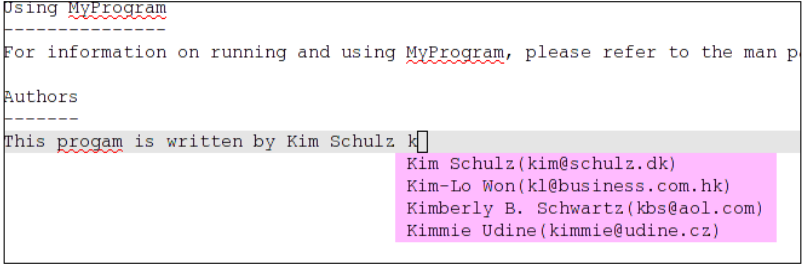
\includegraphics[scale=0.55]{./images/page89.png}
\end{center}
按 \key{Ctrl+o} 可以循环遍历列表中的条目. 另外, 还可以用 \key{Ctrl+n} 向前遍历,
用 \key{Ctrl+p} 向后遍历.

\subsection{多合一补全}
\label{subsec:all_in_one_completion}

用户可能不想记住这么多的补全快捷键, 为什么就不能为所有的补全类型只使用一个快捷
键呢? Vim 可以帮助你实现这个愿望, 现在来看一下具体要怎么做.

大部分支持补全的编辑器通常把这个功能映射到 \key{Tab} 键.

通过下面这个命令, 用户可以在 Vim 的帮助系统中找到一个叫作
\texttt{CleverTab()} 的函数:
\begin{vimcode}
:help ins-completion
\end{vimcode}
这个函数可以让用户使用 \key{Tab} 键来补全单词, 而非 \key{Ctrl+n}. 函数可以自动
区分是应该插入一个制表符, 还是应该做补全操作. 如果用户是在一行的开始, 或者是
某个空白符的后面按下 \key{Tab} 键, 那就是插入一个制表符. 在其他的情况下, 函数
会试图完成已知单词的补全.

借用帮助系统中的 \texttt{CleverTab} 函数, 并对它加以扩展, 使得它可以从下
面的, 带有优先级的列表中选择补全方法:
\begin{itemize}
    \item omnicompletion
    \item 字典补全
    \item 已知单词的补全
\end{itemize}
\marginpar{90}
下面是实现该函数的一个例子:
\begin{vimcode}
function! SuperCleverTab()
	'check if at beginning of line or after a space
    if strpart( getline('.'), 0, col('.')-1 ) =~ '^\s*$'
      return "\<Tab>"
    else
		" do we have omni completion available
       if &omnifunc != ''
		" use omni-completion 1. priority
          return "\<C-X>\<C-O>"
       elseif &dictionary != ''
			" no omni completion, try dictionary completio
			return "\<C-K>"
		else
			"use omni completion or dictionary completion
			"use known-word completion
          return "\<C-N>"
      endif
    endif
endfunction

" bind function to the tab key
inoremap <Tab> <C-R>=SuperCleverTab()<cr>
\end{vimcode}

把函数的代码与按键绑定添加到 \texttt{vimrc} 中, 然后用户就可以用 \key{Tab} 键来
完成各种类型的补全.

按下 \key{Tab} 键进行补全时, 函数检查此时是否是要插入一个制表符. 如果不是, 那
就检查 omnicompletion 函数 (通过 \texttt{omnifunc} 设置) 是否可用. 如果函数不
可用, 那就检查字典是否可用. 如果字典还是不可用, 那就使用最简单的已知单词补全.

\section{宏录制}
\label{sec:using_macro_recording}

编辑具有单一结构的文本时, 或许最好的功能就是录制一段输入宏, 然后再重复执行宏.

完成这个工作的接口非常简单, 更强大的是, 几乎任何东西都可以录制, 接下来我们就
来介绍这个强有力的工具.
\marginpar{91}

先看一下将会用到的命令:
\begin{itemize}
    \item \texttt{qa}: 从现在开始录制, 并记录到寄存器 \texttt{a}. 可以使用任意
        的寄存器, 用寄存器 \texttt{a} 只是为方便起见.
    \item \texttt{q}: 如果是在正在录制时按下, 则停止录制
    \item \texttt{@a}: 执行记录在寄存器 \texttt{a} 中的宏 (可以把 \texttt{a}
        替换成其他的寄存器)
    \item \texttt{@@}: 执行上一次所执行的宏命令
\end{itemize}
可以在 \texttt{@} 前加上任意的数字, 表示重复执行该命令多少次. 例如,
\texttt{15@a} 表示把寄存器 \texttt{a} 中所记录的命令重复执行 15 遍.

先看一个普通的录制会话过程:
\begin{vimcode}
qq
command1
command2
....
commandN
q
10@q
\end{vimcode}
读者可能会好奇这有什么用, 因为这只是在重复执行一串命令罢了. 这种问题最好通过
例子来说明.

想像一下用户有一大串的信息需要处理, Unix 系统的日志文件就属于这种类型. 日志文件
的内容类似于:
\begin{vimcode}
Mar 20 17:23:54 Inspiron kernel: [33604.866998] ath9k 0000:09:00.0: no hotplug settings from platform
Mar 20 17:23:54 Inspiron kernel: [33604.867007] pcieport 0000:00:1c.7: no hotplug settings from platform
Mar 20 17:23:54 Inspiron kernel: [33604.867015] ehci-pci 0000:00:1d.0: no hotplug settings from platform
Mar 20 17:23:54 Inspiron kernel: [33604.867020] ehci-pci 0000:00:1d.0: using default PCI settings
Mar 20 17:23:54 Inspiron kernel: [33604.867039] lpc_ich 0000:00:1f.0: no hotplug settings from platform
Mar 20 17:23:54 Inspiron kernel: [33604.867043] lpc_ich 0000:00:1f.0: using default PCI settings
Mar 20 17:23:54 Inspiron kernel: [33604.867063] ahci 0000:00:1f.2: no hotplug settings from platform
Mar 20 17:23:54 Inspiron kernel: [33604.867067] ahci 0000:00:1f.2: using default PCI settings
Mar 20 17:23:54 Inspiron kernel: [33604.867084] pci 0000:00:1f.3: no hotplug settings from platform
Mar 20 17:23:54 Inspiron kernel: [33604.867089] pci 0000:00:1f.3: using default PCI settings
...
\end{vimcode}
\marginpar{92}

现在, 用户想要把这个日志文件转换成 HTML, 并以表格的形式呈现数据, 看起来就像:
\begin{vimcode}
<tr><td>Oct 8 21:23:34</td><td>laptopia</td><td>kernel:</td><td>ACPI...</td><tr>
\end{vimcode}

用户可以选择一行一行地编辑文件, 直到最后一行. 但也可以这样做, 先编辑一行, 并把
编辑命令录制下来, 然后再把录制下来的命令应用到剩下的每一行. 最开始的编辑命令可
以是下面这些 (假设光标原来是在第一行的开始):
\begin{center}
    \begin{tabular}{ll}
    \hline
    \texttt{qa}             & 开始录制, 并把内容记录到寄存器 \texttt{a} 中 \\
    \texttt{i<tr><td>[ESC]} & 切换到插入模式, 插入 HTML 标记, 再回到普通模式 \\
    \texttt{/ [CR]}         & 向前搜索空格 \\
    \texttt{3n}             & 向前搜索到第 3 个空格 \\
    \texttt{xi</td><td>[ESC]}& 删除空格, 切换到插入模式, 添加 HTML 标记, 再切换
        到普通模式 \\
    \texttt{n}              & 前进到下一个空格 \\
    \texttt{xi</td><td>[ESC]}& 删除空格, 切换到插入模式, 添加 HTML 标记, 再切换
        到普通模式 \\
    \texttt{n}              & 前进到下一个空格 \\
    \texttt{xi</td><td>[ESC]}& 删除空格, 切换到插入模式, 添加 HTML 标记, 再切换
        到普通模式 \\
    \texttt{A</td></tr>[ESC]}&在行的末尾添加 HTML 标记, 再切换到普通模式 \\
    \texttt{j\^}            & 前进到下一行的开始 \\
    \texttt{q}              & 宏录制结束 \\
    \hline
\end{tabular}
\end{center}

\begin{warning}
    \texttt{[ESC]} 指的是按下转码键: \key{Esc}, \texttt{[CR]} 指的是按下回车键:
    \key{Enter}.
\end{warning}

宏准备好了, 光标的位置也已就位, 现在可以重复地执行宏, 并且在每次执行完宏后,
光标都会处在就绪的位置上.

用户可以用 \texttt{@a} 回放存放在寄存器 \texttt{a} 中的宏, 除此之外, 用户还
需要做的就是添加 HTML 的头部与尾部信息, 这很简单.
\marginpar{93}
这只是宏应用的一个简单示例, 如果读者认真回忆一下, 可能会想到更多的, 可以用宏
来优化的工作.

\section{使用会话}
\label{sec:using_sessions}

不知读者有没有想过, Vim 会为你保存多少信息. Vim 保存的信息涵盖了大量的内容, 其
中包括:
\begin{itemize}
    \item 打开的文件, 缓冲区, 窗口, 和标签页
    \item 历史命令
    \item 文本的变化点
    \item 选择与撤消分支
    \item 窗口, 分割 与 GUI 窗口的大小
    \item 光标的位置
\end{itemize}

保存的信息可以分为三类:
\begin{itemize}
    \item 第一类设置信息称为视图 (view), 该类信息应用到一个单独的窗口上. 一个视
        图可以被存储和还原, 因此每当用户使用视图时, 窗口都会呈现出相同的外观.
    \item 第二类设置信息称为会话 (session). 它是一系列视图的集合, 再加上视图
        之间如何配合的信息. 和视图一样, 会话也可以保存下来, 以便于稍后检索.
    \item 剩下的其他信息都归为第三类, 也就是所有的, 不能直接应用到任意一个窗口
        的全局设置. 这些设置可以用会话保存下来, 因此它们也可以保存/还原.
\end{itemize}

接下来的小节将会介绍如何在日常的工作中运用会话.

\subsection{简单的会话使用}
\label{subsec:simple_session_usage}

在使用会话的过程中, 最经常做的事就是把当前正在运行的会话 (如果没有经过特别的设
置, 则是默认会话) 保存到会话文件中, 这样就可以在需要时重新加载会话. 保存会话
的命令是:
\begin{vimcmdform}
\texttt{:mksession}\ \textit{file}
\end{vimcmdform}
保存当前视图的命令是:
\begin{vimcmdform}
\texttt{:mkview}\ \textit{file}
\end{vimcmdform}
\marginpar{94}
命令中的 \textit{file} 是用户指定的, 用于保存会话或视图的文件名. 如果没有指定该
参数, 则默认保存到当前工作目录的 \texttt{Session.vim} 文件中.

\begin{warning}
    如果文件事先存在, 为了覆盖掉文件原来的内容, 需要在 \texttt{mksession} 的末
    尾紧跟上一个感叹号 \texttt{!}.
\end{warning}

使用视图时, 用户可以同时拥有多个不同的视图. 如果每个视图都保存到当前工作目录下, 那
么用不了多长时间, 工作目录就会被视图文件填满. 为了避免这个问题, 可以用下面的命令
告诉 Vim, 应该把视图文件放到哪个目录下:
\begin{vimcode}
:set viewdir=$HOME/.vim/views
\end{vimcode}
上面的命令会把所有的视图文件保存到目录 \texttt{\$HOME/.vim/views}.

假设用户当前打开了三个窗口, 在退出 Vim 之前, 用户执行了:
\begin{vimcode}
:mksession
\end{vimcode}
在下一次准备打开文件时, 用户希望用相同的会话来启动 Vim, 此时可以用命令行选项
\texttt{-S}:
\begin{vimcode}
vim -S Session.vim
\end{vimcode}

除此之外, 用户也可以选择在启动 Vim 后, 用下面的命令来加载会话文件:
\begin{vimcode}
:source Session.vim
\end{vimcode}

对于视图, 加载方式是:
\begin{vimcode}
:loadview View.vim
\end{vimcode}

加载一个会话会改变编辑器的整体布局, 而加载一个视图则只会改变当前活动窗口的布局.
\marginpar{95}
\begin{warning}
    用户如果希望 Vim 记住所有的设置信息, 比如光标的位置与折叠信息, 那么就需要在
    \texttt{vimrc} 中添加如下内容:
    \begin{vimcode}
    set viewdir=$VIMHOME/views/
    autocmd BufWinLeave * mkview
    autocmd BufWinEnter * silent loadview
    \end{vimcode}
    无论何时在同一个窗口中打开另一个缓冲区, 之前的缓冲区的视图都会被自动保存下来,
    并且当再次打开之前的缓冲区时, 会自动还原保存的视图.
\end{warning}

会话的一个常用技巧是定义一个命令, 命令的功能是在退出 Vim 时自动保存会话, 而在打开 Vim
时自动还原保存的会话. 使用这个方法就可以让用户在不丢失设置, 已打开文件列表等
信息的前提下, 自由地启动与退出 Vim. 为了完成这个功能, 可以在 \texttt{vimrc} 中
添加如下命令:
\begin{vimcode}
autocmd VimEnter * call LoadSession()
autocmd VimLeave * call SaveSession()
function! SaveSession()
   execute 'mksession! $HOME/.vim/sessions/session.vim'
endfunction

function! LoadSession()
   if argc() == 0
      execute 'source $HOME/.vim/sessions/session.vim'
   endif
endfunction
\end{vimcode}
关闭 Vim 后, 会话保存到 \texttt{\$HOME/.vim/sessions/session.vim}.

根据打开 Vim 方式的不同, 或者是打开由命令行参数指定的文件, 或者是打开最后一次
会话. 比如说:
\begin{itemize}
    \item \texttt{vim file.txt}: 这种打开方式不会加载最后一次会话.
    \item \texttt{vim}: 这种打开方式会加载最后一次会话, 之前打开的文件会再次
        被打开.
\end{itemize}

如果用户希望在会话文件中存放更多的信息, 可以把额外的信息存放到额外的会话文件中.
方法是创建一个其名字类似于会话文件的文件, 不过要把扩展名 \texttt{.vim} 改成
\texttt{x.vim}. 例如, \texttt{Session.vim} 的额外会话文件是
\texttt{Sessionx.vim}. 额外的会话文件应该和其所属的会话文件放在同一目录下. 用户
可以把想要添加的命令全写到这个文件中, 当 Vim 加载会话文件时, 会把额外的会话
文件中的命令执行一遍.
\marginpar{96}

\subsection{满足个人的会话需求}
\label{subsec:satify_you_own_session_needs}

用户可能并不需要会话文件中存放的所有信息, 有时, 用户可能仅仅是想要保存打开过
的文件的信息, 而在其他时候, 可能是所有的会话信息. 幸运的是, Vim 提供了设置
保存会话信息的方法.

所使用的设置命令是 \texttt{sessionoptions}, 使用方法是:
\begin{vimcmdform}
\texttt{:set sessionoptions=}\textit{options}
\end{vimcmdform}
\textit{options} 是一个由逗号分隔的列表, 列表中可以出现下列选项:
\begin{center}
    \begin{tabular}{lp{35em}}
        \hline
        \textbf{\texttt{blank}}  & 保存空白窗口 \\
        \textbf{\texttt{buffers}} & 保存所有缓冲区的信息, 包括隐藏的与未加载的缓冲区 \\
        \textbf{\texttt{curdir}} & 保存当前工作目录的相关信息 \\
        \textbf{\texttt{folds}} & 保存缓冲区内容中的折叠信息 \\
        \texttt{globals} & 保存全局变量的相关信息, 这里的全局变量指的是以大写
        字母开始, 且类型为字符串或数值的变量 \\
        \textbf{\texttt{help}} & 保存帮助窗口 \\
        \texttt{localoptions} & 保存用户在单个窗口中创建的局部变量与局部映射的
        相关信息 \\
        \textbf{\texttt{options}} & 保存所有的选项信息, 包含全局的与局部的 \\
        \texttt{resize} & 保存 UI 窗口的尺寸信息 (行数与列数) \\
        \texttt{sesdir} & 如果设置了该选项, 当前目录就会是会话文件的存放目录
        (如果同时设置了 \texttt{curdir}, 则该选项不可用) \\
        \texttt{slash} & 把所有文件路径中的反斜杆换成斜杆 (这样做就可以让 Unix
        兼容 Windows 的文件路径) \\
        \textbf{\texttt{tabpages}} & 保存所有的标签页信息, 如果没有设置该选项, 则只会保
        存当前处于活跃状态的标签页 \\
        \texttt{unix} & 使用 Unix 格式的行结束符, 而非 Windows 格式 \\
        \texttt{winpos} & 保存 UI 窗口的屏幕位置信息 \\
        \textbf{\texttt{winsize}} & 保存所有打开窗口的尺寸 \\
        \hline
    \end{tabular}
\end{center}
\marginpar{97}
粗体显示的是 Vim 的默认设置选项. 每次设置选项时并不需要全部设置, 可以通过运算符
\texttt{+=} 和 \texttt{-=} 来增加或移除选项. 比如说, 用户想要在默认选项的基础上
添加 \texttt{winpos}, 并移除 \texttt{folds}, 可以这样做:
\begin{vimcode}
:set sessionoptions+=winpos
:set sessionoptions-=folds
\end{vimcode}
用下面的命令显示当前的会话选项:
\begin{vimcode}
:echo &sessionoptions
\end{vimcode}

\begin{warning}
    实际上, 用户可以用该方法查看所有的 Vim 设置: 通过执行命令 \texttt{:echo},
    并在选项名的前面加上 \texttt{\&}, 比如 \texttt{:echo \&somesessting}.
\end{warning}

\subsection{会话与项目管理}
\label{subsec:sessions_as_a_project_manager}

有时候, 用户可能想要把会话文件作为某种原始的项目文件来使用, 这些项目文件包含了
项目的相关信息. 因此, 如果用户正在处理某个项目, 并且打开了大量的文件与窗口, 只需
执行:
\begin{vimcode}
:mksession!
\end{vimcode}
该命令会把当前会话保存到当前工作目录的 \texttt{Session.vim} 文件中. 如果用户希望
在启动 Vim 时, 自动加载会话文件 (如果存在的话) , 可以把下面这行命令添加到
\texttt{vimrc}:
\begin{vimcode}
silent source! Session.vim
\end{vimcode}
添加了该命令之后, 如果在当前工作目录中存在 \texttt{Session.vim} 文件, 就可以自
动加载. 所以, 只要让会话文件保持在项目目录中, 用户就可以方便把项目加载到 Vim,
但是请记住, 如果打开了新文件, 或者是修改了窗口/缓冲区, 都需要重新保存会话文件.
\marginpar{98}

这只是把会话应用到项目管理的简单用法, 当然, 还有更高级的方法. Wenzhi Liang 开
发了一个实用的脚本, 在 Gvim 的菜单中添加了一个 Project 菜单项. 通过这个菜单项,
用户可以把当前会话保存为以项目命名的文件, 之后, 再通过点击菜单来还原项目, 还
可以在不同的项目之间切换. 如果用户不再需要某个项目, 还可以通过菜单来删除该项目
的会话文件.
\begin{center}
    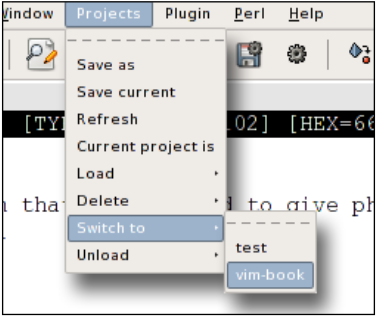
\includegraphics[scale=0.6]{./images/page98.png}
\end{center}

关于该脚本的更多信息, 以及下载地址, 见:
\url{http://www.vim.org/scripts/script.php?script_id=279}

\begin{warning}
    该脚本要求系统中安装了 Perl 与 Bash.
\end{warning}

\section{寄存器与撤消分支}
\label{sec:registers_and_undo_branching}

用户可能都有过这种体验: 刚刚才删除完一段文本, 可是过了一会儿发现, 其他地方还需
要那段文本; 或者是已经复制/剪切了一段文本, 但是过了一会儿之后, 之前复制/剪切的文
本就不见了, 因为剪贴板只能存放一段文本, 后面的文本会把前面的文本给覆盖掉 ---
Vim 是不会让这种事情发生的.

当用户修改文本, 并且需要跟踪被删除/复制的文本, 又或者是跟踪通常情况下对文本作
出的修改时, 可以使用 Vim 提供的两个工具:
\begin{itemize}
    \item 寄存器: 寄存器是一种带有多个缓冲区的高级剪贴板, 可以用来存放被剪切,
        删除或复制的文本.
\marginpar{99}
    \item 撤消分支: 撤消分支是 Vim 版本控制的一种简单形式. 利用撤消分支, 用户
        可以把文件回滚到某个特定的时刻, 或者是回滚一定的次数. 如果用户对某些
        撤消操作感到后悔, 还可以回过头来找到包含这些修改的撤消分支.
\end{itemize}

接下来的两节将会向读者介绍如何在日常的工作中运用寄存器与撤消分支. 读完
之后, 读者将会认识到它们的强大之外, 以及它们在日常工作是如何帮助用户的.

\subsection{使用寄存器}
\label{subsec:using_registers}

在许多程序与操作系统中, 用户只能利用一个剪贴板来完成文本的剪切与复制. 在 Vim 中
不会出现这种情况, 因为用户可以访问多达 9 种不同的剪贴板, 更准确来说, 应该是 9
种不的寄存器类型.

有些寄存器类型的工作领域有所重叠, 但还有一些则拥有自己独特的目的. 用户可以在多
种不同的命令或操作中 (比如复制, 删除, 粘贴) 使用寄存器. 寄存器的名字都以双引号
\texttt{"} 开始, 比如 \texttt{"x}, 所以, 现在来看一下如何使用一个寄存器.
假设现在要用的寄存器是 \texttt{"x}, 至于 \texttt{x} 实际上是表示哪个寄存器,
稍后解释.

为了把某段文本复制到寄存器中, 可以用命令 \texttt{y} 来完成, 不过这次有所不同,
在复制之前, 先告诉 Vim 被复制文本的存放位置:
\begin{vimcmdform}
\texttt{"xy} (用 \texttt{"xyy} 可以复制一整行)
\end{vimcmdform}
对于用来剪切文本的命令 \texttt{x} 也是一样的:
\begin{vimcode}
"xx
\end{vimcode}
对于删除文本的命令 \texttt{d} 则是:
\begin{vimcode}
"xd
\end{vimcode}

现在, 用户已经在寄存器 \texttt{"x} 中存放了一段文本, 并且想要把这段文本粘贴到
正式文本中, 可以用命令 \texttt{P} (粘贴在光标位置之前) 或 \texttt{p} (粘贴在
光标位置之后), 但在粘贴之前, 要先指定寄存器:
\begin{vimcmdform}
\texttt{"xP} 或 \texttt{"xp}
\end{vimcmdform}
\marginpar{100}

如果用户忘记自己使用了哪些寄存器, 可以执行命令:
\begin{vimcode}
:registers
\end{vimcode}

现在, 用户已经知道了如何在基本命令中使用寄存器, 那么接下来将会分别介绍每
一种寄存器类型.

\subsubsection{匿名寄存器}
\label{subsubsec:the_unnamed_register}

之所以称为匿名寄存器, 是因为它只能通过 \texttt{""} 来访问. 每当用户使用命令
\texttt{y} 复制文本, 或者是用 \texttt{d} (删除), \texttt{c} (删除, 并进入插入
模式), \texttt{s} (替换), \texttt{x} (剪切) 删除文本时, Vim 都会自动填充该寄存
器. 匿名寄存器始终指向最近使用的寄存器, 也就是说, 即使用户在删除/复制文本时,
指定了一个特定的寄存器, 匿名寄存器也可以正常工作. 比如说, 命令 \texttt{"xdd}
会把被删除的文本同时存入寄存器 \texttt{x} 与匿名寄存器.

如果用命令 \texttt{p} 或 \texttt{P} 粘贴文本时没有指定寄存器, 那么 Vim 就从匿名
寄存器获取被粘贴的文本.

\subsubsection{行内删除寄存器}
\label{subsubsec:the_small_delete_register}

如果用户删除的文本小于一行, 那么 Vim 就把删除的文本存入一个特殊的寄存器 --- 行
内删除寄存器 \texttt{"-}, 前提是用户没有指定其他的寄存器.

\subsubsection{带编号的寄存器}
\label{subsubsec:the_numberred_registers}

带编号的寄存器包括 \texttt{"0}, \texttt{"1}, 一直到 \texttt{"9}. 带编号的寄存
器分为两类, 第一类是寄存器 \texttt{"0}, 它总是包含了最近一次被删除 (\texttt{d}
或 \texttt{x})/修改 (\texttt{c}) 的文本. 如果用户删除或修改了新的文本, 寄存器
\texttt{"0} 的内容就会被新文本覆盖.

类似于寄存器 \texttt{"0}, 寄存器 \texttt{"1} 也包含了最近一次被删除/修改的文本.
然而, 如果用户指定了其他的寄存器, 又或者是文本的长度少于一行 (此时会自动使用
行内删除寄存器), 那么寄存器 \texttt{"1} 的内容就不会被覆盖. 为了和 vi 兼容, 如
果在删除/修改文本时, 使用下面这些移动命令: \verb'%', \verb'(', \verb')',
\verb'{', \verb'}', \verb'`', \verb'/', \verb'?', \verb'n', \verb'N', 那就总是
使用寄存器 \texttt{"1}, 如果文本少于一行, 还会把文本存入寄存器 \texttt{"-}.
\marginpar{101}

和寄存器 \texttt{"0} 有所不同的是, 寄存器 \texttt{"1} 的内容并不会因为新内容的
加入而被删除, 相反, 原有的内容会移到寄存器 \texttt{"2}. 如果寄存器 \texttt{"2}
原来是非空的, 那么寄存器 \texttt{"2} 的内容会先移到寄存器 \texttt{"3}, 以此类推,
直到寄存器 \texttt{"9}. 寄存器 \texttt{"9} 的原有内容会由于新内容的加入而被覆
盖掉. 通过这种方式, 寄存器 \texttt{"1} 到寄存器 \texttt{"9} 就可以记住删除/修
改的历史内容, 即使用户删除了新的文本, 也可以通过这 9 个寄存器访问到早先被删除
的文本.

\subsubsection{命名寄存器}
\label{subsubsec:the_named_registers}

命名寄存器分为两种 --- \texttt{"a} 到 \texttt{"z} 与 \texttt{"A} 到
\texttt{"Z}.

如果使用的是小写字母的寄存器, 比如 \texttt{"a}, 那么它们就像普通的寄存器那样
工作 --- 将删除或复制的文本存入该寄存器. 当有新的内容被添加进来时, 寄存器中原
来的内容就会被覆盖掉.

如果使用的是大写字母的寄存器, 比如 \texttt{"A}, 那么当有新的内容被添加进来时,
原来的内容并不会被覆盖掉, 而是把新内容追加到原有内容的末尾.

\begin{warning}
    如果往选项 \texttt{coptions} 添加新值 \texttt{'>'}, 那么追加到大写字母寄
    存器的新文本与旧文本之间将会以换行符分开, 给选项设置新值的命令是:
    \texttt{:set coptions+='>'}.
\end{warning}

因为用户对命名寄存器具有完全的控制力, 因此用户应该最先熟悉如何使用它们.

\subsubsection{只读寄存器}
\label{subsubsec:the_read_only_registers}

有四个只读寄存器, 它们的特殊之外在于只有 Vim 才有权限修改它们. 用户只能
通过命令 \texttt{P}, \texttt{p} 或 \texttt{:put} 访问它们的内容. 四个只读寄
存器存放的内容有所不同:
\begin{itemize}
    \item \texttt{"\%}: 该寄存器包含了当前活动缓冲区的文件名.
    \item \texttt{"\#}: 该寄存器包含了当前活动缓冲区上一次打开的文件, 也被称为
        备选文件.
    \item \texttt{".}: 该寄存器总是包含了最近一次插入的文本. 因此, 用户可以通
        过执行 \texttt{".p} 来重复粘贴最近一次插入的文本.
\marginpar{102}
    \item \texttt{":}: 该寄存器包含了用户上一次在命令行执行的命令. 如果用户重
    复执行一条历史命令, 那么寄存器的内容就不会被覆盖. 为了使被执行的命令存入
        该寄存器, 用户至少需要输入命令中的一个字符.
\end{itemize}

\subsubsection{选择与投递寄存器}
\label{subsubsec:the_selection_and_drop_registers}

这种寄存器类型包含了三个寄存器: \texttt{"*}, \texttt{"+} 与 \verb'"~'. 这 3
个寄存器用于存放与检索用户在 Gvim 中选择的文本. 寄存器 \texttt{"*} 实际上访问
的是窗口系统的剪贴板. 如果使用的操作系统是 Miscrosoft Windows, 那么用户在使用
寄存器 \texttt{"*} 与 寄存器 \texttt{"+} 并不会感到有什么不同. 然而, 如果是
Linux, 那就不一样了, 因为 X11 (Linux 的窗口系统) 的选择寄存器不止一个, 而是三
个. 寄存器 \texttt{"+} 存放的是用户所选择的任意一段文本, 典型的选择方式是通过
鼠标完成. 然而, 仅当用户显式地告诉 Vim 去复制文本时, 寄存器 \texttt{"*} 的内
容才会改变.

任意一个 GUI 应用程序都可以访问这些寄存器, 它们的使用方法和日常的复制粘贴没
什么区别.

最后一个寄存器 \verb'"~' 称为投递寄存器, 它包含了最近一次投递到 Vim 的文本.
所以说, 如果用户在另一个程序中选择了一段文本, 并把它拖动到 Vim 的窗口中, 那么
寄存器 \verb'"~' 就包含了这段文本.

\subsubsection{黑洞寄存器}
\label{subsubsec:the_black_hole_register}

顾名思义, 这个寄存器就像黑洞那样工作 --- 进入该寄存器的任意内容都无法再被取
回. 如果用户希望彻底删除某些文本, 也不想让任意一个寄存器记录被删除的文本, 此
时就可以用黑洞寄存器. 黑洞寄存器的名字是 \texttt{"\_}, 使用寄存器的例子有
\texttt{"\_x} 或 \texttt{"\_dd}. 如果用户试图读取刚刚写入到该寄存器的内容, 将
会发现, 无论如何尝试, 都不会返回任何内容.

\subsubsection{搜索模式寄存器}
\label{subsubsec:search_pattern_register}

无论何时使用命令 \texttt{/}, 被搜索的模式都会自动存入搜索模式寄存器. 寄存器
的名字 \texttt{"/} 非常容易记忆, 因为它就是在搜索命令 \texttt{/} 前加上了双
引号, 表明这是一个寄存器. 如果打开了选项 \texttt{hlsearch}, Vim 就会根据寄存
器中的内容来高亮文本. 用户可以利用这个特点, 修改寄存器的内容, 从而高亮显示
其他文本. 在不执行搜索的前提下修改寄存器内容的方法是:
\footnote{原文是 \texttt{:let "/ = }\textit{pattern}, 应该是笔误. --- 译者注}
\marginpar{103}
\begin{vimcmdform}
    \texttt{:let @/="}\textit{pattern}\texttt{"}
\end{vimcmdform}
命令中的 \textit{pattern} 是 \texttt{hlsearch} 将要高亮显示的字符串.

\subsubsection{表达式寄存器}
\label{subsubsec:the_expression_register}

Vim 的最后一种寄存器类型是表达式寄存器, 然而, 称它为寄存器并不恰当, 因为它并不
像其他通常的寄存器那样存放文本, 用户甚至不能写该寄存器. 取而代之的是, 它允许用
户访问命令行, 对表达式求值并返回运算结果, 就好像它一开始就存放在寄存器中似的.

访问表达式寄存器的方式是输入它的名字 \texttt{"=}. 输入完等号后, 光标自动跳转
到命令行窗口, 如果命令行窗口的第一个字符是等号, 则说明用户现在工作在表达式寄
存器. 现在用户可以输入待求值的表达式, 并以回车键结束, 之后, 可以用命令
\texttt{p} 或 \texttt{:put} 把运算结果粘贴到正文中. 如果不想对已输入的表达式
进行求值, 则按 \key{Esc} 结束. 如果用户在按回车键之前没有输入表达式, Vim 就会
使用上一次输入的表达式. 表达式必须是有效的, 而且应该返回一个字符串. 如果表达式
的结果是数值, Vim 会自动把它转换成字符串. 如果用户无法确定运算结果的类型, 可以
使用函数 \texttt{string()} 把结果转换成字符中再返回.\footnote{对表达式寄存器更
方便的用法是: 在插入模式下, 按 \texttt{<c-r>=} (按组合键 \textit{Ctrl+R}, 再
按等号), 接着输入待求值的表达式, 输入完按回车键, 运算结果就会自动插入到正文中.
--- 译者注}

\begin{warning}
    执行 \texttt{:help expression}, 查看如何输入有效的表达式.
\end{warning}

\subsection{撤消分支}
\label{subsec:using_undo_branching}

用户应该都执行过对已修改文本的撤消操作. 通常情况下, 执行撤消操作的方式是按工具
栏的撤消按钮, 或者是组合键, 这样, 最后一次对文本的修改就会被撤消.

在这一方面, Vim 走得更远一些, 而且新增了对分支的支持.

这一节介绍什么是撤消分支, 以及如何在日常工作中使用它.
\marginpar{104}

先来介绍一下什么是撤消分支. 假设现在有一个文件, 而用户已经在它上面作了很多
修改, 这时, 用户突然意识到最后四次更改是错误的. 通常来说, 这时用户会执行四次
撤消命令 (或者直接执行 \texttt{4u}), 这样的话, 最后四次更改就会被取消. 在这里
执行的撤消操作和其他编辑器中的撤消操作没什么不同. 假设现在用户想要对文件作另
一个更改, 比如说改正一个拼写错误.

如果用户此时修改了拼写错误, 那么, 一般来说, 之前被撤消的四次更改操作, 其信息
都会被丢掉 --- 不过 Vim 并不会这样做.

当用户撤消了四次修改, 并添加了一个新修改时, Vim 会在撤消分支树上添加一条新分
支, 此时的撤消分支树看起来就像:
\begin{vimcode}
        A-B-C-D
        /
    E-F-G-H
\end{vimcode}

其中一条分支包含了四个已经被撤消的修改, 另一条分支则包含了最近几次的修改 (拼
写改正). 如果用户继续编辑文本 (不包含撤消操作), 那么撤消树中就只会有这两条分
支. 如果用户在撤消某些操作后, 又作了新的修改, 撤消树就会新增一条分支. 到了最
后, 用户将会看到一棵长满分支的撤消树, 它包含了所有的撤消与编辑操作.

下面这个命令可以查看当前存在着的撤消分支的概览:
\begin{vimcode}
:undolist
\end{vimcode}
命令会显示分支的三种信息 --- 修改号 (用于标识一条分支), 分支所包含的修改的次
数, 分支上最后一次修改发生的时间, 命令的输出信息就像:
\begin{vimcode}
number  changes time ~
6       5       12:12:11
11      8       14:01:15
\end{vimcode}

如果用户想要切换到某个特定的修改号, 执行:
\begin{vimcmdform}
\texttt{:undo }\textit{n}
\end{vimcmdform}
命令中的 \textit{n} 是修改号.
\marginpar{105}

可以用下面的命令在修改列表中后退:
\begin{vimcmdform}
    \texttt{g-}(如果是前进的话, 则是 \texttt{g+})
\end{vimcmdform}

那么, \texttt{g-} 与 \texttt{u} 之间有什么区别? 让我们通过例子来说明.

在 Vim 的编辑区中输入下面的文本:
\begin{vimcode}
My name is Jim
\end{vimcode}
把光标移动到跳到字母 \texttt{J}, 按三次 \texttt{x} 来删除名字 \texttt{Jim},
文本变成了:
\begin{vimcode}
My name is Jim
My name is im
My name is m
My name is 
\end{vimcode}
现在, 用户突然意识到正确的名字是 \texttt{Jimmy}, 于是他撤消了修改:
\begin{vimcode}
My name is m
My name is im
My name is Jim
\end{vimcode}
撤消之后, Vim 中已经有了一条删除名字 \texttt{Jim} 的撤消分支. 现在把名字改为
\texttt{Jimmy}:
\begin{vimcode}
My name is Jimm
My name is Jimmy
\end{vimcode}
但是, 用户真正的名字其实是 \texttt{Kim}, 而非 \texttt{Jimmy}. 因为 \texttt{Jim}
已经和 \texttt{Kim} 很接近了, 所以用命令 \texttt{u} 回滚, 并把 \texttt{J} 改成
\texttt{K}:
\begin{vimcode}
My name is Jimm
My name is Jim
My name is im
My name is Kim
\end{vimcode}
把 \texttt{Jim} 回滚到 \texttt{Jimmy} 后, 会新增一条撤消分支.

现在, 用命令 \texttt{g-} 在修改列表中后退:
\begin{vimcode}
My name is Kim
My name is im
\end{vimcode}
\marginpar{106}
(从这里开始, Vim 切换到一条新的分支)
\begin{vimcode}
My name is Jim
My name is Jimm
My name is Jimmy
\end{vimcode}
(从这里开始, Vim 切换到一条新的分支)
\begin{vimcode}
My name is 
My name is m
My name is im
My name is Jim
\end{vimcode}
如果用的是命令 \texttt{u}, 则变化过程是:
\begin{vimcode}
My name is Kim
My name is im
My name is Jim
My name is Jimm
My name is Jimmy
My name is Jim
\end{vimcode}
可以看到, 命令 \texttt{u} 只是单纯地撤消施加上文本上的修改, 并不理会分支的变化.
而命令 \texttt{g-} 则会按照分支来进行撤消.

简单来说, 撤消分支使得用户可以访问到文本曾经经历过的任何状态.

除了在分支中一步一步地回退之外, 还可以直接跳转到某个时间点的文本状态. 为了完
成这个功能,
Vim 提供了两个命令, 分别用来在撤消历史中向前跳转和向后跳转, 命令的执行形式是:
\begin{vimcmdform}
\texttt{:earlier }\textit{N}\texttt{s} \\
\texttt{:earlier }\textit{N}\texttt{m} \\
\texttt{:earlier }\textit{N}\texttt{h} \\
\texttt{:later }\textit{N}\texttt{s} \\
\texttt{:later }\textit{N}\texttt{m} \\
\texttt{:later }\textit{N}\texttt{h}
\end{vimcmdform}
命令中的 \textit{N} 表示跳过的秒数(\texttt{s}), 分种数 (\texttt{m}), 或小时数
(\texttt{h}). 命令 \texttt{:undolist} 可以显示分支上最后一次修改发生的时间, 通
过这个信息, 用户可以大致计算出需要跳过的时间长度.
\marginpar{107}
熟悉撤消分支的使用可能会需要点时间, 可是一旦上手之后, 它会对用户的日常工作产生
极大的帮助.

\section{折叠}
\label{sec:folding}

一般来说, 编辑大型文件时 (尤其是源代码文件), 用户很难获取一份好的概览. Vim 提
供了一个特性可以解决这个问题 --- 折叠文本块. 这一节介绍如
利用折叠获取文本内容的概览.

折叠指的是将一个范围内的行 (比如一个函数的定义) 折叠成一行, 但不丢失文本内容.
比如折叠下面的文本:
\begin{vimcode}
function myFunction() {
    var a = 1;
    var b = 0;
    var c = a + b;
    return c;
}
\end{vimcode}
折叠后的效果类似于:
\begin{vimcode}
+-- 6 lines: function myFunction() {
\end{vimcode}
在这个示例中, 折叠是根据代码的语法, 用花括号来判断被折叠的范围. Vim 可以根据
下面的信息来折叠文本:
\begin{itemize}
    \item 手动折叠: 由用户手动标出被折叠的范围 (见 \texttt{:help fold-manual})
    \item 缩进折叠: 根据缩进来折叠文本 (见 \texttt{:help fold-indent})
    \item 表达式折叠: 根据表达式来折叠文本 (见 \texttt{:help fold-expr})
    \item 语法折叠: 根据语法来折叠文本 (见 \texttt{:help fold-syntax})
    \item 差异折叠: 折叠未被修改的文本 (见 \texttt{:help fold-diff})
    \item 标记折叠: 根据文本中插入的标记来折叠文本 (见
        \texttt{:help fold-marker})
\end{itemize}
具体使用哪一种指示信息取决于文本的类型, 以及用户的具体操作.
\marginpar{108}

现在开始介绍如何完成折叠操作, 在这之前, 要做的第一件事是打开折叠选项:
\begin{vimcode}
:set foldenable
\end{vimcode}
打开后, Vim 就会注意到在普通模式下输入的折叠命令. 用来打开和关闭折叠的命令有很
多个, 主要的有:
\begin{itemize}
    \item \texttt{zc}: 关闭一个折叠
    \item \texttt{zo}: 打开一个折叠
    \item \texttt{zM}: 关闭所有的折叠
    \item \texttt{zR}: 打开所有的折叠
\end{itemize}
假设把语法折叠作为折叠时的指示信息, 首先把光标移动到需要折叠的区域 (比如某
个函数的内部), 切换到普通模式, 执行命令 \texttt{zc} 来关闭折叠, 现在, 用户就可
以看到函数的定义代码被折叠成一行. 下面的图片显示了折叠与未折叠的代码:
\begin{center}
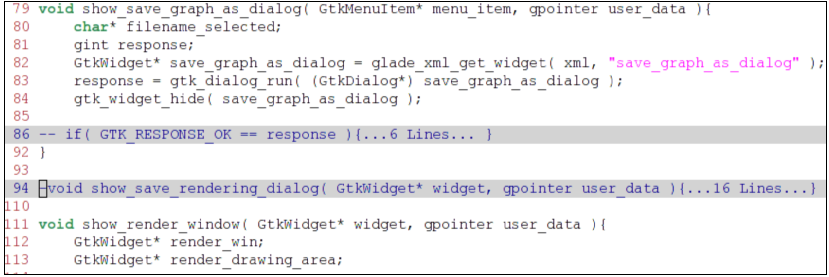
\includegraphics[scale=0.55]{./images/page108.png}
\end{center}

\begin{warning}
    如果用户不想记住打开与关闭折叠的命令, 可以把打开或关闭折叠的切换命令绑定
    到一个按键上, 比如空格: \texttt{:nnoremap <space> za}
\end{warning}

如果用户觉得折叠后的行无法提供自己想要的信息, 可以通过修改选项
\texttt{foldtext} 的值来改变折叠行所显示的信息. 修改的方式是让
\texttt{foldtext} 指向另一个函数, 这个函数返回用户希望看到的信息:
\begin{vimcode}
:set foldtext=MyFoldFunction()
\end{vimcode}
函数 \texttt{MyFoldFunction()} 的实现代码是:
\marginpar{109}
\begin{vimcode}
function! MyFoldFunction()
	let line = getline(v:foldstart)
	" cleanup unwanted things in first line
	let sub = substitute(line, '/\*\|\*/\|^\s+', '', 'g')
	" calculate lines in folded text
	let lines = v:foldend - v:foldstart + 1
	return  v:folddashes.sub.'...'.lines.' Lines...'.getline(v:foldend)
endfunction
\end{vimcode}
函数使得折叠后的行变成:
\begin{vimcode}
+--function myFunction() {...6 Lines...}
\end{vimcode}

用户可以看到函数中使用了三个以 \texttt{v:} 开始的变量, 这些变量由 Vim 设置,
分别包含了:
\begin{itemize}
    \item \texttt{v:foldstart}: 被折叠的第一行的行号
    \item \texttt{v:foldend:}: 被折叠的最后一行的行号
    \item \texttt{v:folddashes}: 为每一层折叠包含一个连字符
\end{itemize}

最后一个变量指出了折叠所在的层次. 假设有这样一段代码:
\begin{vimcode}
if (x != y) {
    if (y != x) {
        print "x not y"
    }
}
\end{vimcode}
最内层 \texttt{if} 的 \texttt{v:folddashes} 将会包含 \texttt{--} (第二层), 而
最外层 \texttt{if} 的 \texttt{v:folddashes} 则是 \texttt{-} (第一层).

折叠行末尾的连字符是自动加上去的. 如果用户希望使用其他字符, 比如等号, 可以这
样做:
\begin{vimcode}
:set fillchars=fold:=
\end{vimcode}

用户可能会感到奇怪为什么需要连字符? 当中的原因其实非常明显. Vim 还有一个称为
\texttt{foldcolumn} 的折叠设置选项, 这个选项说明了应该使用文本左边的多少列
来显示折叠信息. 选项实际上是用这些列画出一个 ASCII 折叠树, 折叠中的连字符就
是树叶. 例如:
\begin{vimcode}
| some text
+- a first level fold
|
    beginning of open fold
2   indication of fold level
2     - do -
- open fold beginning level 1
+-- a second level fold.
| more text
| more text
\end{vimcode}
\marginpar{110}

正如用户所看到的那样, Vim 用 ASCII 字符画出了一棵树:
\begin{vimcode}
|
+-
|
+--
|
+-
+--
\end{vimcode}
下面的命令可以设置树的宽度:
\begin{vimcmdform}
\texttt{:set foldcolumn=}\textit{n}
\end{vimcmdform}
命令中的 \textit{n} 是一个 0 到 12 之间的数, 如果折叠的层次比较少, 推荐使用 1
或者 2; 否则的话, 推荐使用 3 到 5.

\begin{warning}
    用户可以对打开或关闭着的所有折叠执行某个命令:
    \begin{itemize}
        \item \texttt{:folddoopen }\textit{cmd}: 对所有未在关闭的折叠中的行
            \footnote{不仅是处在打开的折叠中的行, 也包括不包含折叠信息的行}
            执行命令 \textit{cmd}
        \item \texttt{:folddoclose }\textit{cmd}: 对所有处在关闭的折叠中的行
            执行命令 \textit{cmd}
    \end{itemize}
\end{warning}

\subsection{提取大纲}
\label{subsec:simple_text_file_outlining}

当用户使用 Vim 编写一个简单的文本文件时, 可能会突然意识到文件已经写得又长又乱
了, 这时候就很需要为文件列一个提纲. 这一节介绍如何使用折叠来为文
件提取大纲, 提取大纲对于改善文件的结构至关重要.

假设文本文件的内容是:
\begin{vimcode}
Chapter 1
Section 1 - Vim help
here is some text about the vim help system.
Section 2 - vim scripts
this section contains info about vim scripts.
\end{vimcode}
\marginpar{111}

现在, 用户想要折叠文本, 使得只有 Section 的头部显示出来. 如果用手动折叠 (
\texttt{:set foldmethod=manual} 则比较方便, 方法是选中 Section 内的所有行 (包
括头部), 然后按下 \texttt{zf}, 就可以把这些行折叠起来. 另外, 用户可以认为
\texttt{Chapter 1} 是第一层折叠, 每一个 Section 是第二层, 关闭 Section 所在的
折叠后应该变成:
\begin{vimcode}
-Chapter 1
+Section 1 - Vim help   (2)
+Section 2 - Vim scripts    (4)
\end{vimcode}

\begin{warning}
    为了达到上面的效果, 需要做如下设置:
    \begin{vimcode}
    :set foldcolumn=1
    :set fillchars=fold:\  "there is a space after the \
    :set foldtext=getline(v:foldstart).'    ('.v:foldstart.')'
    \end{vimcode}
\end{warning}

经过这样的处理之后, 文件看起来就像是书籍的目录, 不同之处是这仅仅是一个普通的文本
文件而已. 只要新增的行是在之前的行的后面, Vim 就仍然会把新增的行当作是折叠的一
部分.

如果想要删除折叠, 只需要在可视模式下选中文本, 再按下 \texttt{zd}.

如果用户想让文本拥有不同的格式 (比如, 用 \texttt{= =} 包围 Section 的头部),
这当然可以实现 --- 只要用户标记了自己的折叠区域, 那么实现起来就不会有什么问题.

\subsection{使用 vimdiff 比较差异}
\label{subsec:using_vimdiff_to_track_the_changes}

有时候, 用户可能拥有同一文件的多个版本 --- 这些版本之间可能相同, 也可能不同.
在 Unix 系统中, 有一个称为 \texttt{diff} 的命令, 这个命令很早就开始被人们使用
(最早出现于 1974 年), 但是其他系统很可能没有该命令. 这个命令的功能是显示两个
文件的差异, Vim 也提供了一个用于比较差异的工具 --- \texttt{vimdiff}. 这一节介
绍如何使用 Vim 比较文件的差异.
\marginpar{112}

\texttt{vimdiff} 是 Vim 内置的差异比较工具, 它使用颜色显示文件间的差异 (被
比较的两个文件分别处在两个纵向切割或横向切割的窗口中). 下面的图片显示了
\texttt{vimdiff} 的工作界面:
\begin{center}
    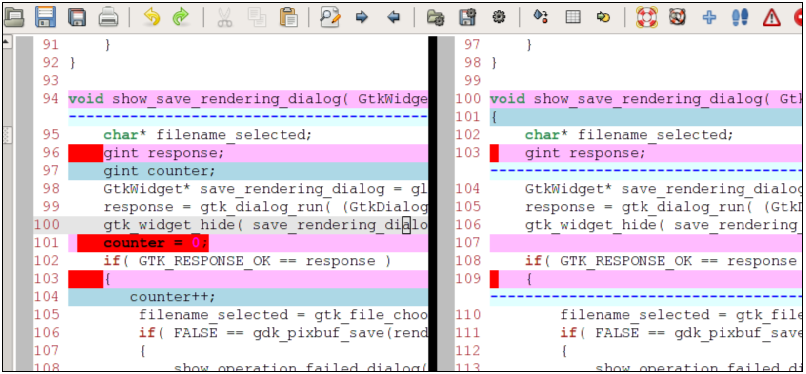
\includegraphics[scale=0.5]{./images/page112.png}
\end{center}

有若干种方式可以用来启动 \texttt{vimdiff}. 在安装了 Vim 的系统中, 一般都有一
个叫作 \texttt{vimdiff} 的程序快捷键, 用户可以通过它启动 \texttt{vimdiff}:
\begin{vimcode}
vimdiff file1 file2
\end{vimcode}
上面的命令行等价于:
\begin{vimcode}
vim -d file1 file2
\end{vimcode}

启动 \texttt{vimdiff} 时至少需要提供两个文件进行比较, 至多可同时比较 4 个文件.

如果用户已经启动了 Vim, 并且想要激活 \texttt{diff} 模式, 那么可以这样做:
\begin{itemize}
    \item \texttt{:diffsplit }\textit{filename}: 水平切割窗口, 并在其中一个窗口
        打开 \textit{filename}, 所有和 \texttt{vimdiff} 相关的设置会同时应用
        到这两个窗口中.
    \item \texttt{:vert diffsplit }\textit{filename}: 垂直切割窗口, 并在其中
        一个窗口中显示 \textit{filename}, 所有和 \texttt{vimdiff} 相关的设置
        会同时应用到这两个窗口中.
    \item \texttt{:diffthis}: 使得当前窗口成为差异窗口的一部分. 当用户想要再
        次对某个文件进行差异比较时, 可能会用到该命令.
\end{itemize}
\marginpar{113}

一个常见的例子是比较当前文件, 与上一次 Vim 所保存的备份之间的差异 (备份文件的
文件名以波浪号 \verb'~' 结尾). 假设用户正在编辑的文件是 \texttt{main.c}, 则
可以在任意时刻保存文件, 然后执行:
\begin{vimcode}
:vert diffsplit main.c~
\end{vimcode}
执行命令后, 窗口被垂直分割成两个, 文件间的差异通过颜色标记出来 (具体的颜色
取决于当前使用着的色彩主题)

还有一种情况是, 对文件作出修改的并不是用户本人,  而是另一个开发人员向用户发
了一个文件补丁, 对于这种情形, Vim 也提供了一个 \texttt{diff} 视图, 用于查看补
丁被应用到文件后所带来的变化. 方法是打开补丁所对应的文件, 然后执行 \texttt{vert
diffpatch }\textit{patchfile}, 或者省略 \texttt{vert}, 直接执行
\texttt{:diffpatch }\textit{patchfile}.

命令中的 \textit{patchfile} 是其他开发人员发送给用户的补丁. 执行命令后,
Vim 会在另一个窗口中打开文件, 把补丁打到该文件上, 然后比较打补丁前, 与打补
丁后文件的差异.

\subsection{在 vimdiff 中导航}
\label{subsec:navigation_in_vimdiff}

和普通的 Vim 窗口相比, 在 \texttt{vimdiff} 窗口中导航会稍有不同.

例如, 滚动其中一个窗口时, 会同时滚动另一个窗口. 实际上, 窗口之间的每一行, 其
相对位置不变, 这是通过选项 \texttt{scrollbind} 来实现的:
\begin{itemize}
    \item 开启同时滚动的命令是:
\begin{vimcode}
:set scrollbind
\end{vimcode}
    \item 关闭同时滚动的命令是:
\begin{vimcode}
:set noscrollbind
\end{vimcode}
\end{itemize}

当在 \texttt{diff} 窗口中编辑文件时, Vim 会自动根据文件内容的变化, 来相应地更
新窗口中的颜色; 如果没有更新, 则可以执行:
\begin{vimcode}
:diffupdate
\end{vimcode}
\marginpar{114}

如果光标正处在某一 \texttt{diff} 窗口中, 而用户希望在修改之间快速地跳转, 这就
需要用到下面的命令:
\begin{itemize}
    \item \texttt{[c}: 跳转到前一个修改的开始
    \item \texttt{]c}: 跳转到下一个修改的开始
\end{itemize}
通过这种方法, 用户可以在文件的相关区域间方便地跳转, 并且可以很容易看出对文件
作了哪些修改.

如果光标正处在 \texttt{vimdiff} 窗口的某一差异上, 而且用户知道该修改对文件的
另一版本也是需要的. 虽然可以把修改复制下来, 并插入到另一个文件的适当位置, 但
是 Vim 提供了比这更方便的做法. 下面这个命令可以把修改应用到同一文件的另一个版
本上:
\begin{vimcode}
:diffput
\end{vimcode}

执行该命令时, 光标必须处在待应用的修改上. 另一方面, 如果光标是处在不含有修改
的文件上, 那么用户可以先跳转到含有修改的文件上, 然后把修改应用到另一个文件,
或者直接使用下面的命令:
\begin{vimcode}
:diffget
\end{vimcode}
除了这两个命令, 还可以在普通模式下使用另外两个替代命令 \texttt{do} 与
\texttt{dp}.

\begin{warning}
    更多的内容请参考 \texttt{:help vimdiff}.
\end{warning}

\subsection{使用 diff 跟踪变化}
\label{subsec:using_diff_to_track_changes}

前面一节已经学习到如何使用 \texttt{vimdiff} 来比较同一文件的不同版本之
间的差异, 但是, 如果用户仅仅是想知道在保存之前, 对当前活动缓冲区作了哪些修
改, 那又应该怎么办呢? 这一节介绍如何查看硬盘上的文件与缓冲区中的文件之间的差
异, 也就是自从上一次保存以来, 文件所发生的变化.
\marginpar{115}
用户所要做的首先是把下面的代码添加到文件 \texttt{vimrc}:
\begin{vimcode}
function! DiffWithFileFromDisk()
	  let filename=expand('%')
	  let diffname = filename.'.fileFromBuffer'
	  exec 'saveas! '.diffname
	  diffthis
	  vsplit
	  exec 'edit '.filename
	  diffthis
	endfunction
\end{vimcode}

函数为当前缓冲区中的文件保存一份临时副本 (包含了最新的修改), 然后对临时文件与
硬盘上的文件进行差异比较.

为了调用这个函数, 需要执行:
\begin{vimcode}
:call DiffWithFileFromDisk()
\end{vimcode}
也可以为调用命令绑定一个快捷键:
\begin{vimcode}
:nmap <F7> :call DiffWithFileFromDisk()<cr>
\end{vimcode}
上面的命令把功能键 \key{F7} 绑定到函数调用, 使用时只需要切换到普通模式, 再按
下 \key{F7}, 就可以看到用 \texttt{diff} 模式标记的修改.

现在, 用户就可以在保存文件之前, 查看所有未保存的修改, 检查是否每个修改都是正确
的.

\section{打开任意位置的文件}
\label{sec:open_files_anywhere}

系统管理员与网站开发人员经常会被同一个问题所困扰, 如果解决得不好的话, 会给人带
来很大的麻烦, 这个问题就是他们所浏览的文件大部分都存放在远程服务器上.

系统管理员对此问题的解决办法通常是远程登录到服务器上 (比如用 ssh (Secure
Shell), 然后再在服务器上直接修改配置文件.

网站开发人员的解决办法通常是先把文件下载到本地, 编辑好后再上传到服务器上, 下
载与上传的工具可以用 FTP 客户端, 或 Webdav.
\marginpar{116}

如果不使用上面提到的方法, 那又应该怎么办呢? 为什么他们就不能在本地直接编辑远程
服务器上的文件? Vim 可以在不需要额外扩展的前提下完成这件事. Vim 含有一个称为
netrw (Net Read/Write) 的系统, 它可以用来编辑远程服务器上的文件,
通过例子介绍如何使用它.

假设有一个网站开发人员, 叫作 John, 他把他的主页放在远程服务器
\texttt{remote.server.com} 上. 现在他想要编辑文件 \texttt{index.html}, 这个文
件存放在服务器家目录下的 \verb'public_html/'. 使用 Vim 打开此文件的命令是:
\begin{vimcode}
vim ftp://john@remote.server.com/public_html/index.html
\end{vimcode}

Vim 根据参数识别出它需要使用 FTP 协议连接到服务器 \texttt{remote.server.com},
所使用的用户名是 \texttt{john}, 如果还需要输入密码, Vim 就会在连接时给出
提示信息. Vim 从服务器上下载一份文件的副本到本地, 用户所编辑的正是该副本, 所
不同的是每当用户保存文件时, Vim 都会同时保存一份到服务器上.

如果 John 已经打开了 Vim, 则可以使用下面两个命令中的一个打开远程服务器上的文
件:
\begin{vimcode}
:Nread ftp://john@remote.server.com/public_html/index.html
:Nread remote.server.com john PASSWORD public_html/index.html
\end{vimcode}
命令中的 \texttt{PASSWORD} 是登录时所使用的密码. 除了可以读取远程服务器上的文
件, 还可以把本地文件写到远程服务器上, 甚至可以在一台服务器上打开文件, 并把它
保存到另一个服务器上. 把文件保存到 FTP 服务器的命令是:
\begin{vimcode}
:Nwrite ftp://user@server/path/to/filename
:Nwrite server user password path/to/filename
\end{vimcode}

\begin{warning}
    针对不同的协议, \texttt{:Nread} 与 \texttt{:Nwrite} 所使用的参数也有所不
    同, 可以通过 \texttt{:Nread ?} 与 \texttt{:Nwrite ?} 查看具体的规则.
\end{warning}

除了 FTP, Vim 还支持以下协议:
\begin{itemize}
    \item SCP
    \item SFTP
    \item RCP
    \item HTTP (只读)
    \item DAV
\marginpar{117}
    \item rsync (只读)
    \item fetch (只读)
\end{itemize}

为了在 Vim 的命令中使用这些协议, 只需要把前面例子中的 \texttt{ftp} 替换成对应
的协议名 (小写形式) 即可.

然而, 有一点需要注意. 为了使用这些协议, Vim 依赖于外部的命令行程序. 在 Linux
系统中, 这些程序默认都是可用的, 但是对于 Miscrosoft Windows 来说, 只有 FTP
是可用的. 为了查看 Vim 所使用的外部程序, 以及如何修改它们, 执行:
\begin{vimcode}
:help netrw-externapp
\end{vimcode}

除了读取与编辑远程文件, Vim 还可以列出远程目录中的所有文件, 这做便于用户选择
正确的文件进行编辑. 为了列出远程目录中的文件, 只需要把 \texttt{:Nread} 的参数
由文件改为目录即可, 例如:
\begin{vimcode}
:Nread scp://user@server/some/directory/
\end{vimcode}
执行命令后, 用户可以选择任意一个文件进行编辑, 就好像它们就在本地目录.

\begin{warning}
    如果是 Linux 系统, 则用户可以把登录远程服务器所用的用户名与密码保存到本地
    家目录的 \texttt{.netrc} 文件中, 更多的信息参考 \texttt{:help netrw-netrc}.
\end{warning}

\subsection{更快的远程文件编辑}
\label{subsec:faster_remote_file_editing}

用户既然已经知道了如何直接编辑远程服务器上的文件, 那么他就很有可能同时打开多个
远程文件. 这时用户就会遇到一个很恼人的情况: 每当移动到另一个缓冲区时 (用命令
\texttt{:bufferprev} 或 \texttt{:buffernext}), 都需要重新登录.

默认情况下, 每次显示缓冲区的文件内容时, Vim 都会尝试重新加载文
件. 也就是说, 如果打开的是一个远程文件, 那么 Vim 就会尝试重新登录, 以检查文件是
否需要重新加载.

但是这真的有必要吗? 如果远程文件除了用户之外, 没有其他人正在编辑, 那么在切换
缓冲区时就不需要重新加载文件.
\marginpar{118}

每一个缓冲区都有一套选项, 指明了在不同的情况下如何处理缓冲区. 其中之一就是
\texttt{bufhidden}, 它表示当缓冲区被隐藏 (在窗口中不可见) 时 Vim 该做什么操作.
默认情况下该选项的值为空, 如果把它设置成 \texttt{hide}, 那就是告诉 Vim 当在
窗口中看不到缓冲区时, 只需把它隐藏即可; 当再次把它显示在窗口中时, 只需把它显示
出来即可. 为了不让 Vim 在切换缓冲区时重新从远程加载文件, 在 \texttt{vimrc} 中
添加:
\begin{vimcode}
set bufhidden=hide
\end{vimcode}

\section{小结}
\label{sec:production_boosters_summary}

这一章介绍了如何在日常工作中更高效地使用 Vim. 介绍了很多方法, 也提出
了一些优化措施.

首先是介绍了如何利用模版来降低文本输入的工作量. 最开始是使用缩写来插入模版,
然后, 是根据不同的文件类型来制作并插入对应的模版文本. 最后, 讨论如何使用
snipMate 脚本来为任意的文件格式制作高级 snippet.

接着是自动补全. 我们介绍了各种不同的补全方法, 还说明了如何把众多补全方法都绑
定到 \key{Tab} 键上.

通过记录一系列命令, 用户就可以多次重复执行同一段命令序列. 说明了如何使用
宏录制, 把日志文件的内容转换成 HTML 格式.

再接下来是 Vim 的会话. 介绍了如何保存窗口的状态, 以及如何把会话用作项目
管理程序.

通过寄存器, 用户可以使用多达 9 个不同的寄存器/剪贴板.

通过折叠文本, 用户能够得到更好的文件概览, 因为无关紧要的部分都被隐藏在了折叠
中. 还可以利用折叠来制作文件的提纲.
\marginpar{119}

文件被修改过了, 但是具体改了哪些地方呢? 我们介绍了如何使用 Vim 内置的
\texttt{diff} 功能. 通过它, 用户可以获取文件修改的概览, 或者是在维持良好的
\texttt{diff} 概览的前提下, 撤消或添加分支.

编辑本地文件是一回事, 编辑远程机器上的文件是另一回事. Vim 可以做到直接编辑
或操作远程文件, 而且和编辑本地文件相比, 用户并不会感到有什么不同.

在下一章, 我们将会学习到如何使用 Vim 的格式化选项来格式化普通文本或代码.
% end of chapter 4

% vim: ts=4 sts=4 sw=4 tw=80
\chapter{格式化进阶}
\label{chap:advanced_formatting}
\marginpar{121}

很多时候, 最简单的工作就是把文本或代码修改成更易阅读的形式. 本章将会
介绍一些简单的方法, 用于对文本进行格式化 --- 无论是普通文本还是代码.

这一章主要分为三个部分:
\begin{itemize}
    \item 文本格式化
    \item 代码格式化
    \item 使用外部格式化工具
\end{itemize}

学完这一章后, 用户应该可以清楚地知道当要对文本进行格式化时, 什么情况下应该用
Vim, 什么情况下不应该用 Vim.

\section{格式化文本}
\label{sec:formatting_text}

在编辑普通文本时, 虽然大多数人更喜欢使用图形化字处理软件, 比如 Microsoft Word
或 OpenOffice, 但是许多纯文本编辑器, 比如 Vim, 也可以把事情做得很好. 在下面的
一节里, 将会介绍如何利用 Vim 强大的功能来格式化普通文本.
\marginpar{122}

\subsection{文本分段}
\label{subsec:putting_text_into_paragraphs}

这一节所介绍的知识可能是整本书中最简单的, 但是对于格式化普通文本来说, 却可能是
最有用的. 假设用户正在编写一段文本, 并且在编写的过程中丝毫没有注意到行的变化与
文本的格式. 最终, 用户可能会写出一行非常长的文本, 此时他才注意到应该对文本重新
进行格式化, 摆在他面前的有两个选择:
\begin{itemize}
    \item 遍历文本, 并在适当的地方断行
    \item 用某个命令对整段文本进行格式化
\end{itemize}
很显然, 后者是最好的选择, 并且格式化后的结果也可以和其他结果保持一致. 所使用的
命令是:
\begin{vimcode}
gqap
\end{vimcode}
上面的命令其时是两个命令的组合:
\begin{itemize}
    \item \texttt{gq}: 把紧接在该命令后的动作所覆盖到的文本进行格式化
    \item \texttt{ap}: 选择一个段落 (``a paragraph'')
\end{itemize}

换句话说, 由 \texttt{gq} 与 \texttt{ap} 组合而成的命令告诉 Vim 去遍历当前段落
并格式化. 由两个空白行包围起来的部分定义为一个段落, 因此, 为了开始一个新的段
落, 只需要添加一个空行即可.

Vim 所做的格式化实际上是让行作出更漂亮的断行, 使得每一行的长度都不会超过某个
特定的大小 (Vim 自动地在适当的两个单词间作出断行).

格式化后文本的宽度由选项 \texttt{textwidth} 定义, 如果用户希望每行最大的宽度不
超过 80 个字符, 那就在 \texttt{vimrc} 中添加:
\begin{vimcode}
:set textwidth=80
\end{vimcode}
如果 \texttt{textwidth} 的值被设置为 0, 那么 Vim 就把它设置成窗口的宽度 ---
但是永远不会多于 \texttt{textwidth} 所设置的字符个数.\footnote{ 原文是
If the option is set to 0, the Vim sets it to the width of the window ---
but never more than the number of characters defined in the the
\texttt{textwidth} setting.}
\marginpar{123}

\begin{warning}
    通过设置选项 \texttt{formatoptions} 可以控制 Vim 如何格式化段落. 更多的信
    息可以参考 \texttt{:help 'formatoptions'} 与 \texttt{:help 'fo-table'}.
\end{warning}

\texttt{gq} 可以和任意的移动命令配合使用, 并且在格式化之后, 光标将会停留在移动
命令结束的地方 (典型的情况是停留在当前特定区域的最后一行). 如果用户希望在格式
化后, 光标仍旧处于格式化开始前的位置, 那就把 \texttt{gq} 改成 \texttt{gw}. 如
果用户的光标原来是在段落中第一行的开始, 此时执行 \texttt{gwap}, 命令结束后, 光
标仍然会停留在段落中第一行的开始.

用户可以在命令的前面加上数字, 使得它重复执行, 例如, \texttt{5gqap} 将会对当前
与下面的四个段落进行格式化. 如果想要对文件内的所有段落进行格式化, 就执行
\texttt{1gqG}.

前面的介绍的格式化命令不仅对普通文本有效, 对其他任意类型的内容同样有效, 而且用
户可以决定使用哪种格式化函数.

用户可以为指定的文件类型设置任意的格式化函数, 方法是设置 Vim 的选项
\texttt{formatexpr}. 例如, 如果用户想要对 C 源代码进行格式化, 只需要在
\texttt{vimrc} 中添加:
\begin{vimcode}
:set formatexpr=c#Formatter()
\end{vimcode}
这行命令告诉 Vim, 在打开一个 C 源代码文件时, 使用函数 \texttt{Formatter()},
这个函数定义在 Vim 为 C 文件自动加载的文件中.

\begin{warning}
    自动加载的文件可以在 \texttt{VIMHOME} 的子目录 \texttt{autoload} 中找到.
    文件根据所服务的文件类型来命令, 以后缀 \texttt{.vim} 结束. 例如, 为 C 文
    件自动加载的文件是 \texttt{VIMHOME/autoload/c.vim}.
\end{warning}

一个格式化函数含有三个变量, 利用这三个变量可以找到待格式化的文本.
\begin{itemize}
    \item \texttt{v:num}: 待格式化的第一行的行号
    \item \texttt{v:count}: 待格式化的行的数量
    \item \texttt{v:char}: 这个变量包含了将被插入的字符, 可以为空
\end{itemize}

格式化函数的一个简单示例是:
\marginpar{124}
\begin{vimcode}
function! MyFormatter()
   let first = v:num
   let last = v:num + v:count
    while(first<=last)
       call setline(first, '> '. getline(first))
       let first = first+1
    endwhile
endfunction
\end{vimcode}
这个格式化文本接收所有的行, 在每一行的开始添加 \texttt{>}, 就像电子邮件中的引
用.

上面展示的格式化函数非常简单, 如果需要更高级一点的, 那么函数的复杂度就会快速
增加, 因此公开可用的格式化函数非常有限 (这些函数是为了某些特定的目标而开发的).

\subsection{对齐文本}
\label{subsec:aligning_text}

在大多数字处理程序中, 最基本的格式化选项之一是左对齐, 右对齐, 或居中. 其中
一些程序甚至可以让文本两端对齐, 这样做可以让每一行的结束尽可能地向边缘靠近.

虽然上面提到的格式化类型对字处理程序来说非常常见, 但对于普通文本编辑器来说就
很少见了, Vim 就位列其中.

Vim 支持三种类型的对齐 --- 左对齐, 右对齐, 居中. 在介绍它们如何工作之前,
先简单解释一下支持这种对齐类型的文本编辑器为什么很少.

对于常见的文本编辑器来说, 它们不含有隐藏信息, 也就是说, 用户所能看到的, 就是
用户所能拥有的 --- 没有页面宽度, 没有对齐, 什么都没有.

另一方面, 在字处理程序中, 文档隐藏了相当丰富的信息, 这些信息告诉编辑器如何
根据用户的需要, 对文本进行格式化.

因为上面所说的情况对 Vim 并不适用, 所以用户得向 Vim 提供一些信息, 来帮助 Vim
进行格式化. 例如, 为了让编辑器知道对齐时所需的边缘, 用户需要设置文本的宽度.

说完了这些, 先来看一下居中排列的命令:
\begin{vimcode}
:[range]center WIDTH
\end{vimcode}
\marginpar{125}
命令中的 \texttt{range} 是用户希望居中的行的范围, \texttt{WIDTH} 是每行最多的
字符数. 典型的用法是在可视模式下选中待居中的文本 (按住 \key{Shift+v}, 然后移
动光标), 然后再输入命令. 按下 \texttt{:} 后, 用户将会发现 Vim 自动地把选中的
文本的范围记成 \texttt{'<,'>}, 这表示从选中文本的第一行到最后一行.

接下来, 用户需要输入 \texttt{center} 与文本的宽度. 如果选项 \texttt{textwidth}
已经设置妥当, 那就不需要输入 \texttt{WIDTH}.

如果选项 \texttt{textwidth} 的值为 0, 用户又没有在命令中设置 \texttt{WIDTH},
那么 Vim 就默认使用 80 个字符的宽度. 在字处理程序中, 用户很容易就可以看出文本
是否是居中的, Vim 对文本进行居中时, 只是在前面加上适当数量的空格, 这样
做意味着无论是在什么时候修改了文本, 用户都要重新对文本进行居中.

下面的命令用于左对齐:
\begin{vimcode}
:[range]left INDENT
\end{vimcode}
同样, 执行这个命令时需要提供行的范围, 如果需要的话, 再提供缩进的宽度. 这个命令
可以用来精确地设置文本的左边边缘.

最后是右对齐命令. 同样的, Vim 可能并不知道一行的宽度, 因此执行命令时还要提供
宽度信息. 命令的形式是:
\begin{vimcode}
:[range]right WIDTH
\end{vimcode}
范围内的行用空格缩进, 使得每一行的结束都是对齐的, 宽度由用户指定. 和居中一样,
无论何时修改了文本, 都要重新对文本进行右对齐.

\subsection{标记标题}
\label{subsec:marking_headlines}

使用普通的文本编辑器编写文档时, 用户可能需要创建自定义的格式或标记, 使得文本
更容易阅读.

为了提高可读性, 一个常见的操作是为那些用作标题的字符串作标记, 这些标题可以是
文本的章节.
\marginpar{126}

如果是字处理程序, 只需要把字体设置得更大更粗就可以了, 但是这样的字体设置对
Vim 却是不可能实现的, 因为 Vim 字体的大小是固定的. 因此, Vim 用户必须通过其他
的方法来标记标题.

笔者个人的选择是在标题的下面添加一行, 来表示这是一个标题行.

一个简单的例子是:
\begin{vimcode}
My Headline
===========
This is the text on the document. It could cantain one
or more lines of text.
\end{vimcode}
不同级别的标题可以用不同类型的标记来表示:
\begin{vimcode}
Level1
======
Level2
------
-Level3-
\end{vimcode}

为了更方便地添加下划线, 在 Vim 中可以用宏来实现, 使用这种方法不用担心下划线添
加得太多或太少.

前面两个级别的标题宏可以实现成:
\begin{vimcode}
yypVr=o
\end{vimcode}
宏的各个部分的具体涵义是:
\begin{itemize}
    \item \texttt{yy}: 复制当前行
    \item \texttt{p}: 粘贴
    \item \texttt{V}: 选中一整行
    \item \texttt{r}: 用后面的字符 (在这里是 \texttt{=}) 替换掉选中的字符
    \item \texttt{o}: 在光标的下面添加一个空行, 把光标移动到这行的开始, 并切
        换到插入模式
\end{itemize}

这个宏的基本功能是获取当前行 (标题行), 并复制它. 然后把复制得到的行的所有字符
替换成某个字符 (在这个例子中是 \texttt{-} 或 \texttt{=}), 最后, 插入一个新行,
并切换到插入模式.

对第三级别的标题来说, 我们必须采取其他办法, 所做的操作无非是在一行的开始
和结束添加一个连字符, 可以用一条替换命令来完成:
\marginpar{127}
\begin{vimcode}
:s/\.(.*\)/-\1-/
\end{vimcode}
把命令拆成三部分来说明:
\begin{itemize}
    \item \texttt{:s///}: 替换命令
    \item \verb'\(.*\)': 正则表达式, 表达式把当前行的所有字符作为输入, 并把
        它们作为搜索模式
    \item \verb'-\1-': 替换模式. 替换模式告诉 Vim 在第一个被匹配的子模式前
        添加一个连字符, 在子模式的后面再加上一个连字符
\end{itemize}

记住, 这些宏可能会写得很复杂, 但我们可以很轻易地为它们绑定一个快捷键, 例如:
\begin{vimcode}
:map h1 yypVr=0
:map h2 yypVr-0
:map h3 :s/\(.*\)/-\1-/
\end{vimcode}
现在, 用户可以在普通模式下, 通过按 \texttt{h1}, \texttt{h2}, \texttt{h3} 来添
适当的标题行. 如果用户不想在标题行的下面添加一个空行并切换到插入模式, 就把上
面的映射命令中的 \texttt{o} 删掉.

\subsection{创建列表}
\label{subsec:creating_lists}

项目列表与编号列表是文档中的常见结构. 本节将会介绍在 Vim 中如何方便
地创建这些列表.

首先来看一个函数, 这个函数接收某个范围内被选中的行, 然后把它们转化成项
目列表. 在这个列子里, 一个简单的项目列表是:
\begin{vimcode}
* first item
* second item
* third item
\end{vimcode}
为每一行的开始添加星号的函数可以是:
\begin{vimcode}
function! BulletList()
    let lineno = line(".")
    call setline(lineno, "    * " . getline(lineno))
endfunction
\end{vimcode}
\marginpar{128}

认真看一下函数的实现, 就会发现它所做的不过是获取当前行, 然后再用它的一份
拷贝替换掉自身, 在前面添加一个空格, 一个星号, 然后是一个制表符.

很显然, 函数只对一行有效, 然而, 如果用户选中了一个范围内的所有行, 那么 Vim 就
会为每一个选中的行调用一次函数, 从第一行, 一直到最后一行. 如果是为每一行添加
相同的内容, 那么这种方法就很方便.

然而, 上面介绍的方法并不适合编号列表, 因为用户必须记住下一个号码从多少开始.

所以, 现在来看下面的函数, 它把某个范围内选中的行转换成编号列表 --- 列表的每一
项都占据一行:
\begin{vimcode}
function! NumberList() range
  " set line numbers in front of lines
  let beginning=line("'<")
  let ending= line("'>")
  let difsize = ending-beginning +1
  let pre = ' '
  while (beginning <= ending)
      if match(difsize, '^9*$') == 0
          let pre = pre . ' '
      endif
    call setline(ending, pre . difsize . "\t" . getline(ending))
    let ending=ending-1
    let difsize=difsize-1
  endwhile
endfunction
\end{vimcode}

这个函数稍微有点复杂, 但和它所解决的问题比起来, 还是比较简单的 --- 在每一行
的开始添加一个数字.

除此之外, 函数还做了一个额外的工作 --- 数字右对齐:
\begin{vimcode}
    1 item1
    2 item2
    ...
   10 item10
   11 item11
    ...
  100 item100
    ...
\end{vimcode}
\marginpar{129}

为了做到这样的对齐, 需要考虑两个问题:
\begin{itemize}
    \item 必须知道列表最大的编号
    \item 必须一次处理所有的行
\end{itemize}

为了解决第一个问题, 必须查看范围内第一行与最后一行的行号, 两个行号之间的差就
是行数, 于是就得到了列表编号的最大值. 由于考虑了第二个问题, 所以这
是唯一可能的解决办法, 如果不这样做的话, 那么函数每次就只能看到当前行.

解决第二个问题的办法是在函数名的后面添加关键字 \texttt{range}, 这个关键字告诉
Vim, 函数是对一个范围内的行作操作, 而不仅仅是一行.

函数从范围内的最后一行处理到第一行, 无论何时碰到一个只含有 9 的数字 (比如 99,
9999), 都说明编号中的字符少了一个 (例如, 从第 1000 行到第 999 行), 为了弥补缺
少的一个字符, 函数为缩进新增一个空格. 通过这种办法, 可以一直保证数字的右对齐,
无论范围内有多少行.

\begin{warning}
    在 \url{http://www.vimoutliner.org}, 用户可以找到利用标题格式化, 列表格式
    化等技术来为文档列提纲的脚本. 如果用户需要在 Vim 中为文档列提纲, 最好试一
    下这个脚本.
\end{warning}

\section{格式化代码}
\label{sec:formatting_code}

在对代码进行格式化时经常需要考虑很多因素. 每一种语言都有自己的语法规则, 还有
些语言对格式非常依赖. 在有些情况下, 程序员需要按照公司给出的规定来格式化代码.

那么, Vim 如何知道用户想把代码格式化成什么样子? 简单来说 Vim 并不需要知道. 但
是 Vim 有办法让用户完全按照自己的需要来格式化代码.
\marginpar{130}

虽然具体的格式化细节不尽相同, 但是它们都遵循一些基本的规则, 也就是说, 用户只
需要关心不同的地方即可. 在大部分情况下, 格式化规则的修改可以通过一系列的 Vim
选项设置, 在这些选项当中, 比较重要的有以下几个:
\begin{itemize}
    \item \texttt{formatoptions}: 这个选项负责特定格式的设置 (见 \texttt{:help
        'fo'})
    \item \texttt{comments}: 什么是注释, 以及如何对它们进行格式化 (见
        \texttt{:help 'com'})
    \item \texttt{(no)expandtab}: 用空格代替制表符 (见 \texttt{:help
        'expandtab'})
    \item \texttt{softtabstop}: 一个制表符可以用多少个空格来代替 (见
        \texttt{:help 'sts'})
    \item \texttt{tabstop}: 一个制表符的宽度 (见 \texttt{:help 'ts'})
\end{itemize}

通过这些选项, 用户几乎可以设置与缩进相关的方方面面. 但是光有这些还不足够,
用户仍
然需要告诉 Vim 是否需要自动缩进, 还是由用户手动完成缩进. 如果用户希望由 Vim
来完成缩进, 可以通过 4 种方法来完成, 下面的小节将会介绍与代码缩进
相关的一系列选项.

\subsection{Autoindent}
\label{subsec:autoindent}

Autoindent 是缩进代码最简单的方式. 它的功能仅仅是与上一行保持相同的缩进层次.
所以说, 如果当前行缩进了 4 个空格, 按下 \key{Enter} 后插入的空行也会缩进 4 个
空格. 至于什么时候修改缩进的层次则完成取决于用户. 这种缩进方式适用于若干行需
要保持相同缩进层次的语言. 打开 autoindent 的命令是 \texttt{:set autoindent}
或 \texttt{:set ai}.

\subsection{Smartindent}
\label{subsec:smartindent}

Smartindent 比 autoindent 稍微智能一些. 它仍然可以让上一行的缩进层次保持到下
一行, 但用户无需手动修改缩进层次. Smartindent 可以识别出 C 语言的大部分结构,
并根据它们来决定何时增加/减少缩进层次. 由于许多编程语言都或多或少地都继承了 C
语言的语法, 所以 smartindent 也可以应用到其他语言. 打开 smartindent 可以用下
面两个命令中的任意一个:
\begin{itemize}
    \item \texttt{:set smartindent}
    \item \texttt{:set si}
\end{itemize}
\marginpar{131}

\subsection{cindent}
\label{subsec:cindent}

Cindent 经常被称为 clever indent(聪明的缩进) 或 configurable indent(可配置的
缩进), 这是因为与前面介绍的两种缩进相比, 它的可配置性更强. 有三种设置选项:
\begin{itemize}
    \item \texttt{cinkeys}: 这个选项包含了一个列表, 列表中的各项之间用逗号分
        开, Vim 可以根据列表中的项来改变缩进层次. 一个例子是: \texttt{:set
            cinkeys="0\{,0\},0\#,:"}, 意思是说无论何时碰到一个以 \verb'{', 或
            \verb'}', 或 \verb'#' 作为开始的行, 或者是以 \verb':' 作为结束的
            行 (很多语言的 \texttt{switch} 结构都用到了 \verb':'), Vim 都要
            再缩进一层. \texttt{cinkeys} 的默认值是 \texttt{"0\{, 0\}, 0), :,
        0\#, !\textasciicircum F, o, O, e"}, 更多的信息见 
        \texttt{:help cinkeys}.
    \item \texttt{cinoptions}: 这个选项包含了所有的, 专门用于 cindent 的选项.
        它是一个各项之间由逗号分开的列表, 通过这个列表可以设置大量的选项. 一
        个例子是 \texttt{cinoptions=">2,\{3,\}3"}, 意思是说在正常的缩进之上,
        再额外添加两个空格, 另外, 在 \verb'{' 与 \verb'}' 的左边添加三个空格,
        以便与前一行作比较. 因此, 如果目前的缩进是 4 个空格, 那么刚才所说的
        设置会使代码变成:
\begin{lstlisting}[
    basicstyle=\ttfamily,
        xleftmargin=2em,
        breaklines=true,
        tabsize=4,
        showspaces=true,
]
if (a == b)
   {
      print "hello";
   }
\end{lstlisting}
        \texttt{cinoptions} 的默认值是 \path{">s,e0,n0,f0,{0,}0,^0,%
        :s,=s,l0,b0,gs,hs,ps,ts,is,+s,c3,C0,/0,(2s,us,U0,w0,W0,m0,j0,%
        )20,*30"}, 更多的信息见 \texttt{:help 'cinoptions'}.
    \item \texttt{cinwords}: 这个选项包含的关键词会让 Vim 在下一行增加缩进. 一
        个例子是 \texttt{:set }\path{cinwords="if,else,do,while,for,switch"},
        这同时也是它的默认值. 更多的信息见 \texttt{:help 'cinwords'}.
\end{itemize}
\marginpar{132}

\subsection{Indentexpr}
\label{subsec:indentexpr}

Indentexpr 是最灵活的缩进选项, 但同时也是最复杂的. 使用 indentexpr 时, 它会
对一个表达式求值, 然后计算出一行的缩进. 因此, 用户写出的表达式必须能被 Vim
求值. 打开这个选项的方法是为它设置一个表达式, 比如:
\begin{vimcode}
:set indentexpr=MyIndenter()
\end{vimcode}
命令中的 \texttt{MyIndenter()} 是一个函数, 负责计算行的缩进.

函数的一个简单例子是模仿选项 autoindent 的功能:
\begin{vimcode}
function! MyIndenter()
   " Find previous line and get it's indentation
   let prev_lineno = s:prevnonblank( v:lnum)
   let ind = indent( prev_lineno )
   return ind
endfunction
\end{vimcode}

即使是想把函数的功能增强一点, 函数的复杂度也会迅速增长. Vim 自带了多种编程语言
的缩进表达式, 如果用户想要自己编写缩进表达式, 可以以它们为基础, 再加以修改. 用
户可以在 \texttt{VIMHOME} 的子目录 \texttt{indent} 中找到实现代码.

更多的信息见 \texttt{:help 'indentexpr'} 与 \texttt{:help 'indent-expression'}.

\subsection{代码块快速格式化}
\label{subsec:fast_code_block_formatting}

缩进选项设置完毕后, 用户可能想根据新设置的选项更新一下代码的格式. 为了更新代码,
只需要告诉 Vim 重新缩进第一行到最后一行, 具体的命令是:
\begin{vimcode}
1G=G
\end{vimcode}
如果把命令拆开来看, 各个部分的意思是:
\begin{itemize}
    \item \texttt{1G}: 跳到文件的第一行 (也可以使用 \texttt{gg})
    \item \texttt{=}: 根据格式化的配置对文本加以缩进
    \item \texttt{G}: 跳到文件的最后一行 (缩进的结束位置)
\end{itemize}
\marginpar{133}

如果把命令映射到按键上, 使用起来就更加方便:
\begin{vimcode}
:nmap <F11> 1G=G
:imap <F11> <ESC>1G=Ga
\end{vimcode}
后一个命令尾巴的 \texttt{a} 是为了在格式化完成后, 重新回到插入模式, 因为在执行
命令前就处在插入模式下. 现在, 只需按下 \key{F11}, 就可以对整个缓冲区的文本重新
缩进.

\begin{warning}
    注意, 如果待缩进的代码含有编程错误, 比如在 C 代码中漏写了一个分号, 那么代
    码就不会被正确地缩进. 利用这个性质可以在一定程序上检查编程错误.
\end{warning}

有时候, 用户可能仅仅是想格式化某一小块代码, 对于这种情况, 用户可以使用代码块
自然形成的范围, 或者是在可视模式下选择一段代码, 然后再格式化.

后一种方法比较简单. 先是切换到可视模式, 比如按下 \key{Shift+v}, 然后再按
\key{=} 来重新缩进被选中的代码行.

另一方面, 如果要使用代码块, 则有多种不同的方法来实现. 在选择代码块时, Vim 提供
了很多的方法. 为了与一个缩进代码的命令作组合, 我们必须介绍这些不同类型的代码
块, 以及选择它们的命令:

\begin{itemize}
    \item \verb'i{': 内部块 (Inner block), 指的是 \verb'{' 与 \verb'}'
        之间的所有内容 (
        不包括 \verb'{' 与 \verb'}'). 还可以用 \verb'i}' 与 \texttt{iB} 来选
        择.
    \item \verb'a{': 一个块 (A block), 指的是 \verb'{' 与 \verb'}'
        之间的所有内容 (包括
        \verb'{' 与 \verb'}'). 还可以用 \verb'a}' 与 \verb'aB' 来选择.
    \item \verb'i(': 括号内 (Inner parenthesis), 指的是 \verb'(' 与 \verb')'
        之间的所有内容 (不包
        括 \verb'(' 与 \verb')'), 还可以用 \verb'i)' 与 \verb'ib' 来选择.
    \item \verb'a(': 一对括号 (A parentheses), 指的是 \verb'(' 与 \verb')'
        之间的所有内容 (包括 \verb'(' 与 \verb')'), 还可以用 \verb'a)' 与
        \verb'ab' 来选择.
    \item \verb'i<': 内部 \verb'<>' 块 (Inner \verb'<>' block), 指的是
        \verb'<' 与 \verb'>'
        之间的所有内容 (不包括 \verb'<' 与 \verb'>'), 还可以用 \verb'i>'
        来选择.
    \item \verb'a<': 一个 \verb'<>' 块 (A \verb'<>' block), 指的是
        \verb'<' 与 \verb'>'
        之间的所有内容 (包括 \verb'<' 与 \verb'>'), 还可以用 \verb'a>'
        来选择.
    \item \verb'i[': 内部 \verb'[]' 块 (Inner \verb'[]' block), 指的是
        \verb'[' 与 \verb']'
        之间的所有内容 (不包括 \verb'[' 与 \verb']'), 还可以用 \verb'i]'
        来选择.
    \item \verb'a[': 一个 \verb'[]' 块 (A \verb'[]' block), 指的是
        \verb'[' 与 \verb']'
        之间的所有内容 (包括 \verb'[' 与 \verb']'), 还可以用 \verb'a]'
        来选择.
\end{itemize}
\marginpar{134}

现在, 我们已经知道了 Vim 是如何看待一个代码块的, 接下来, 只需要告诉它如何
操作代码块, 在这个例子中, 是希望 Vim 重新缩进代码块. 前面已经说到,
\texttt{=} 可以用来重新缩进代码, 所以重新缩进代码块的一个示例是:
\begin{vimcode}
=i{
\end{vimcode}
用上面的命令重新缩进下面的代码 (\verb'|' 表示光标的当前位置):
\begin{vimcode}
if( a == b )
  {
    print |"a equals b";
  }
\end{vimcode}
执行命令后, 代码变成 (默认使用 C 语言的缩进格式):
\begin{vimcode}
if( a == b )
  {
    print |"a equals b";
  }
\end{vimcode}
如果改用 \verb'a{' 来选择代码块, 代码就会变成:
\begin{vimcode}
if( a == b )
  {
    print "a equals b";
  }
\end{vimcode}
在最后一段代码中, 命令 \verb'=a{' 同时纠正了花括号与打印语句的缩进.

有时候, 用户可能会遇到一个带有多级代码块的代码块, 并且用户希望重新缩进当前代码
块及包围它的代码块. 不用担心, Vim 提供了一个很方便的做法. 比如, 如果用户想要重
新缩进当前代码块及包围它的代码块, 只需要把光标放在相对内层的代码块上, 并执行:
\begin{vimcode}
=2i{
\end{vimcode}
这个命令告诉 Vim 重新缩进内层代码块中的两层, 从当前 ``活跃'' 的块到该块的外层.
可以把命令中的 \texttt{2} 替换成用户想要重新缩进的层数. 当然, 还可以把
\texttt{i} 替换成其他的代码块选择命令, 从而精确地选择待缩进的代码块.

上面介绍的这些, 就是缩进代码所要掌握的全部内容.
\marginpar{135}

\subsection{自动格式化粘贴的代码}
\label{subsec:auto_format_pasted_code}

经常有程序员告诉我, 他们会经常复用已有的代码, 这意味着他们经常需要复制与粘
贴代码.

许多用户在把代码粘贴到 Vim 窗口中时, 都会碰到过 ``阶梯效应'' --- 当插入代码时,
Vim 会尝试对代码进行缩进, 造成的结果是越往后, 行的缩进层次越深, 类似于阶梯:
\begin{vimcode}
code line 1
    code line 2
        code line 3
            code line 4
               ...
\end{vimcode}
解决这个问题的办法通常是把 Vim 设置成 粘贴 (paste) 模式, 用到的命令是:
\begin{vimcode}
:set paste
\end{vimcode}
代码粘贴完毕后, 用下面的命令把 Vim 设置回正常的插入模式:
\begin{vimcode}
:set nopaste
\end{vimcode}

那么, 除此之外, 是否还有其他的方法呢? Vim 是否可以根据文件中已有的其他代码来
自动格式化被粘贴的代码? 其实很简单.
\begin{vimcode}
p=`]
\end{vimcode}
上面的命令只是把普通的粘贴命令 (\texttt{p}) 和另一命令组合, 后者会自动缩进前
面插入的行 (\texttt{=`]}). 这个命令基于下面的事实: 当用户使用命令 \texttt{p}
来粘贴文本时, 光标将会停留在被粘贴文本的第一个字符上, 组合上命令 \texttt{`]}
之后, 光标就会移动到最近一次插入的文本行的最后一个字符上, 并且可以从被粘贴文
本的第一行移动到最后一行.

所以, 用户所要做的就是把这个命令绑定到一个快捷键上, 并用该快捷键来粘贴文本.
\marginpar{136}

\section{使用外部格式化工具}
\label{sec:using_external_formatting_tools}

即使是经验丰富的 Vim 用户也会经常说 Vim 可以做任何事情, 虽然事实上并不是这样,
但其实已经很接近了 --- 对于 Vim 不能做的事, 最好借助外部工具来完成.

下面的小节介绍最经常使用的格式化工具, 以及如何使用它们.

\subsection{Indent}
\label{subsec:indent}

程序 Indent 可能是最常使用的 Vim 外部工具. 从 80 年代开始, 它就被安装到了各种
不同的 Unix 平台中, 后来还被移值到了 Microsoft Windows.

顾名思义, 这个程序的功能就是缩进代码 --- 特别是那些类 C 代码. 用户可
会感到奇怪 --- 既然 Vim 本来就可以缩进代码, 而且做得也很不错, 那干嘛还要用外
部工具呢? 这个问题非常好, 答案是 Vim 确实在这一方面做得很好, 但是 Indent 做得
更好, 并且更容易在多个编辑器之间对缩进进行标准化.

由于 indent 专门用于缩进代码, 所以它的效率和 Vim 相比会高出很多, 对于后者来
说, 缩进代码只是一项特性而已, 而不是唯一的特性. Indent 对代码的理解力很高, 可
以根据代码来缩进 --- 即使含有语法错误.

那么, 在 Vim 中应该如何使用 Indent? 前面的几节已经介绍了 Vim 关于缩
进的几个选项, 然而, 现在只需要一个选项即可:
\begin{vimcmdform}
\texttt{:set equalprg=}\textit{program}
\end{vimcmdform}

这个选项的功能是当使用命令 \texttt{=} 缩进代码时, Vim 应该使用哪种外部工具.
对于
Indent, 只要把 \textit{program} 替换成程序 Indent 的路径即可. 设置之后, 无论
何时使用缩进命令 (比如 \texttt{1G=G}), Vim 就会把待缩进的文本输送给程序
Indent. 甚至可以在选项中加上命令行选项.

Indent 有着非常丰富的命令行选项, 另外还可以通过它的配置文件来修改 Indent 的
行为.
\marginpar{137}

\begin{warning}
    可以从以下网址下载到最新版的 Indent:
    \url{http://www.gnu.org/software/indent/}.
\end{warning}

\subsection{Berkeley Par}
\label{subsec:berkeley_par}

90 年代早期, Adam M. Costello 开始开发一个简单的命令行工具, 这个工具的唯一功
能是按照用户的要求, 重新格式化文本中的段落. 工具的名字是 Par, 一两年后, 该工
具拥有了非常丰富的功能, 几乎可以重新格式化任意类型的段落.

正因为如此, Par 成了 Vim 的理想工具, 现在介绍一些使用示例.

假如, 用户想重新格式化段落, 使得每一行最大长度不超过 78 个字符, 那就在 Vim 中
执行:
\begin{vimcode}
:set formatprg=par\ -w78
\end{vimcode}

选项 \texttt{formatprg} 告诉 Vim, 当使用命令 \texttt{gq} 时, 应该调用哪个外部
工具来格式化文本. 值得注意的是, 程序和它的参数之间的空格用一个反斜杆转义, 这
做就可以让 Vim 把程序与它的参数看作一个整体.

\begin{warning}
    注意, 如果 \texttt{formatexpr} 为空, 则只会使用 \texttt{formatprg}, 否则
    的话, 就使用 \texttt{formatexpr}.
\end{warning}

前面曾经提到过, Vim 无法对文本进行两端对齐, 幸运的是, Par 可以帮助 Vim
完成这件工作. 只需要在上面的命令行参数中加上 \texttt{j} (意思是 justify),
就可完成两端对齐:
\begin{vimcode}
:set formatprg=par\ -w78j
\end{vimcode}

Par 不仅可以用在普通文本中, 对于代码的某些部分也可以使用, 比如注释.

假设用户拥有下面一段注释:
\begin{vimcode}
/********************************************************************/
/* This function helps you modify a string and remove all */
/* unnecessary characters . */
/* Don't use this on widechar strings or strings shorter than 10 */
/* characters */
/********************************************************************/
\end{vimcode}
\marginpar{138}
用户可以选中这些注释, 然后执行:
\begin{vimcode}
!par 60r
\end{vimcode}
(Vim 会在 \texttt{!} 的前面自动加上 \texttt{'<,'>})

执行后, 注释变成:
\begin{vimcode}
/**********************************************************/
/* This function helps you modify a string and remove all */
/* unnecessary characters . Don't use this on widechar    */
/* strings or strings shorter than 10 characters          */
/**********************************************************/
\end{vimcode}

只需要一个简单的命令, 用户就可以把丑陋的, 未格式化过的注释变成精心排列的文本.

Par 的手册页包含了许多例子.

\begin{warning}
    读者很容易就可以把不同的 Par 命令映射到不同的按键上去, 通过这种办法, 可
    以为所有的文本, 注释, 线性表等设置格式化快捷键.
\end{warning}

\subsection{Tidy}
\label{subsec:tidy}

如果用户从事网页开发, 或者 XML 文件编辑, 那么程序 tidy 就会成为你的好帮手. 这
个程序可以清理代码, 使之符合 W3C 规范. 符合 W3C 规范指的是代码的构造必须遵守
由 W3C 规定的 HTML 守则.

作为一个网页开发人员, 笔者有时候会浏览别人写的 HTML 或 XML 文件, 打开后只看
到了一团乱麻. 后来, 笔者会在打开之前, 先用 tidy 处理一下所有的 \texttt{.xml},
\texttt{.html} 或 \texttt{.html} 文件. 这个工作可以借助 Vim 的自动命令来完成,
自动命令可以添加在文件 \texttt{vimrc} 中.

对于 XML 文件, 自动命令的具体代码是:
\begin{vimcode}
au FileType xml exe ":silent 1,$!tidy --input-xml true --indent yes -q"
\end{vimcode}
对于 HTML 文件, 自动命令是:
\begin{vimcode}
au FileType html exe ":silent 1,$!tidy --indent yes -q"
\end{vimcode}
\marginpar{139}
需要注意得是, 这个命令会在打开文件时悄无声息地修改掉文件内容. 在上面两个命令
中, Vim 会在指定的路径中搜索程序 tidy, 无论是 Linux 还是 Windows.

观察 tidy 的命令行参数后可以看到, 它也可以用来重新缩进 HTML/XML. 这个选项提高
了文件的可读性, 也更容易获取文件的概览.

因为 tidy 可以检查出文档的错误, 所以用户可以把 tidy 的命令映射到一个键上, 这
样的话就可以随时检查文档是否符合 W3C 规范.

\begin{warning}
    可以到 \url{http://tidy.sourceforge.net} 下载到最新版的 tidy.
\end{warning}

\section{小结}
\label{sec:advanced_formatting_summary}

本章介绍了如何更好地格式化普通文本与代码.

首先, 我们介绍了如何通过一对简单的 Vim 命令, 把文本格式化成更易阅读的形式.
还介绍了文本的对齐, 还解释了纯文本编辑器在对齐方面的困难. 接下来, 我们创建
了一个函数, 该函数用于标记标题行, 以及生成无编号与编号列表. 我们还看到了 Vim
非常的灵活, 比如用户可以告诉 Vim 是否需要对选中的文本中的每一行执行操作, 又或
者是是否让用户来处理, 并将待处理的行一次都反馈给用户的函数.

接下来介绍了在 Vim 中如何格式化代码, 尤其是缩进. 因为每个人都有
着自己独特的编码风格, 所以很难有一个通用的功能来完成代码的格式化. Vim 提供了
一个灵活的接口, 使得用户可以按照自己的需要来设置. 我们还介绍了一些用来迅速格
式化代码的技巧, 甚至还包括如何格式化从其他地方粘贴到 Vim 中的代码.

最后, 介绍了如何利用外部工具来使得 Vim 更加完美. 外部工具可以帮助用户格式
化文本与代码, 我们介绍了几种比较流行的外部工具, 以及在 Vim 中使用它们的方法.
\marginpar{140}

到了这里, 用户应该可以熟练地利用 Vim 内建功能, 使得它更符合自己的需求. 接下来,
读者将学习到如何编写 Vim 脚本.
% end of chapter 5

% vim: ts=4 sts=4 sw=4 tw=80
\chapter{Vim 脚本基础}
\label{chap:basic_vim_scripting}
\marginpar{141}

Vim 的一个最强大之处是允许高级用户通过编写脚本增强 Vim 的功能. 通过脚本, 用
户几乎可以往 Vim 中添加任意功能, 而且很容易与其他用户分享.

这一章会介绍编写 Vim 脚本的基础知识, 讨论的主题包括:
\begin{itemize}
    \item 编写语法高亮脚本
    \item 安装与使用脚本
    \item 不同类型的脚本
    \item 如何开发脚本
    \item Vim 脚本的基本语法
    \item 在 Vim 脚本中使用其他脚本语言
\end{itemize}

学习完这一章之后, 对于如何使用 Vim 脚本, 读者应该会有一个基本的概念, 而且有能
力写出一个简单的脚本, 从而为 Vim 添加新的功能.

\section{语法高亮方案}
\label{sec:syntax_color_schemes}

在许多程序员看来, 根据语法来高亮代码是 Vim 最重要的特性之一. 语法高亮不仅使代码
看起来更清晰, 还可以帮助用户发现编码错误. Vim 语法高亮系统所使用的脚本非常像
Vim 脚本, 但是语法高亮脚本定义的是颜色, 而不是功能. 下一节介
绍如何创建一个语法高亮方案.
\marginpar{142}

\subsection{第一个语法高亮文件}
\label{subsec:your_first_syntax_color_file}

简单来说, 语法高亮的关键是识别出文本中的特定单词与结构, 然后再给它们设置上对
应的颜色. 然而, 大部分情况下要稍微复杂一点, 因为语法高亮还要识别上下文语境.
假设现在要语法高亮下面的代码:
\begin{vimcode}
/* if x equals y then return the value */
if (x == y)
  {
    return x;
  }
\end{vimcode}

如果仅仅是根据单词与符号来匹配, 那也可以得到一个相当不错的结果. 下面是具体
的配置命令 (每个选项的意义已经在第 \ref{chap:personalizing_vim} 章中进行了介
绍):
\begin{vimcode}
:syntax keyword myVars x y
:syntax match mySymbols "[{}();=]"
:syntax keyword myKeywords if return
:highlight myVars ctermfg=red guifg=red
:highlight mySymbols ctermfg=blue guifg=blue
:highlight myKeywords ctermfg=green guifg=green
\end{vimcode}

\begin{center}
    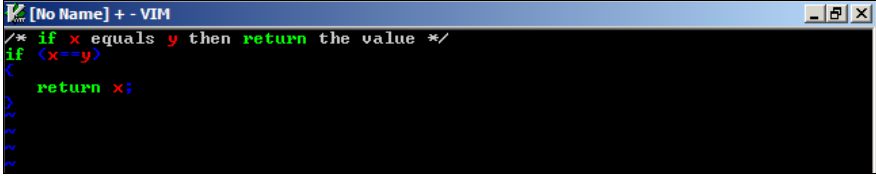
\includegraphics[scale=0.5]{./images/page142.png}
\end{center}

从上图中可以看到, 代码部分的高亮还不错, 可是注释语句却不令人满意. 这是因为我们
只是对单个单词进行匹配, 所以注释中的相同单词也会被匹配. 这种配置方法很难分辨出
代码与注释.
\marginpar{143}

那么, 我们可以从这个简单的例子里学习哪些东西呢? 那就是, 与高亮比起来, 更重要的
是要找到期望中的单词, 然后再给它们设置对应的颜色. 现在增加一些上下文的信
息, 把 \verb'/*' 与 \verb'*/' 之间的部分标记成注释, 然后再高亮其余的部
分. 代码部分被标记上颜色之后, 就不需要再上色了, 因此规则的顺序很重要. 具体的
配置代码是:
\begin{vimcode}
:syntax match myComments "/\*.*\*/"
:syntax keyword myVars x y
:syntax match mySymbols "[{}();=]"
:syntax keyword myKeywords if return
:highlight myVars ctermfg=red guifg=red
:highlight mySymbols ctermfg=blue guifg=blue
:highlight myKeywords ctermfg=green guifg=green
:highlight myComments ctermfg=yellow guifg=yellow
\end{vimcode}
最终的效果是:
\begin{center}
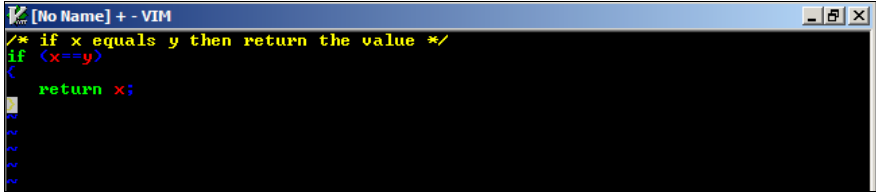
\includegraphics[scale=0.5]{./images/page143.png}
\end{center}

现在, 这段代码的高亮已经相当得体. 当然, 这只是一个小例子, 而且只用到了 Vim 语
法高亮的一小部分功能, 接下来将会介绍更多的内容.

\section{区域高亮}
\label{sec:syntax_regions}

前面的例子是用选项 \texttt{match} 来选择注释语句. 在某些情况下,
我们很难创建一个适当的匹配语句, 这时候, 就需要用到其他一些更方便的做法.

在 Vim 中, 用户可以选中一整个代码区, 然后再高亮它们, 为了选择一个代码区, 只需要
提供区域的开始与结束. 对于前面的例子, 如果使用区域高亮的话, 具体的命令是:
\begin{vimcode}
:syntax region myComments start=/\/\*/ end=/\*\//
\end{vimcode}
\marginpar{144}
有了这个命令, 很轻易就能匹配下面的任意一个注释块:
\begin{vimcode}
/* single line comment */
/*******************************
 *  multi line comments
 *******************************/
/* multi line comment
 */
\end{vimcode}

除了设置区域开始与结束, 选项 \texttt{region} 还可以做更多的事. 它还可以根据其
他语法规则来高亮区域内的某些代码. 笔者常做的一个操作是为函数注释设置几个关键词,
比如 \texttt{FIXME}, \texttt{OBSOLETE}, \texttt{TODO}, 等等, 这样, 我就可以把
代码写成:
\begin{vimcode}
/*  function: splitString()
 *  args    : string
 *  OBSOLETE
 */
function splitString(string) {
...
\end{vimcode}
剩下的工作, 就是创建一个关键词组:
\begin{vimcode}
:syntax keyword myKeywords OBSOLETE FIXME TODO
\end{vimcode}
现在, 需要修改命令 \texttt{region} 的设置, 以允许区域内包含其他语法元素,
修改后的命令是:
\begin{vimcode}
:syntax region myComments start=/\/\*/ end=\/\*\// contains=myKeywords
\end{vimcode}

如果需要在区域内包含多于一个的语法组, 只需要把它们写成列表的形式 (列表元素之间
用逗号分开), 再写到 \texttt{contains} 的后面.

\begin{warning}
    只有当开始与结束都在同一行时, 你才能告诉 Vim 这个区域是正确的, 方法是在
    命令 \texttt{syntax} 中添加一行选项. 如果没有这个选项, Vim 会在遇到开始时
    就开始高亮代码, 遇到结束时 (或者是文件的末尾) 停止.
\end{warning}
\marginpar{145}

在某些情况下, 用户可能希望在一个区域中嵌套另一个区域, 对于这种情况, 用户必须
把这项需求显式地告诉 Vim, 方法是在区域命令的末尾加上选项 \texttt{contained}:
\begin{vimcode}
:syntax region myComments start=/\/\*/ end=\/\*\// contains=myKeywords
contained
\end{vimcode}

在某些情况下, 一个代码块可以出现在代码中的任意一个位置, 当然, 用户不想针对每
一个代码块各写一个语法组, 这时候, 只需要把 \texttt{contains} 改成 \texttt{ALL}.

除了 \texttt{ALL}, 其他的关键词还包括:
\begin{itemize}
    \item \texttt{ALLBUT}: 如果它是列表的第一项, 那么列表中的其余项目在区域中
        都不会被高亮显示
    \item \texttt{CONTAINED}: 如果该项在列表中, 那么带有选项 \texttt{contained}
        的语法组就会在区域中被高亮显示
    \item \texttt{TOP}: 如果该项在列表中, 那么除了带有选项 \texttt{contained}
        的语法组, 其他所有的语法组都会被包含进来
\end{itemize}

有了上面的帮助, 用户就可以轻易地选择大范围的语法组, 而不用一个一个地把它们写下
来. 一个例子是选择除了 \texttt{myComments} 之外的所有语法组, 具体的命令是:
\begin{vimcode}
:syntax region myCodeblock start=/{/ end=/}/ contains=ALLBUT,myComments
\end{vimcode}

\begin{tips}
    如果用户知道某些语法组经常一起使用, 可以把它们放在一个簇 (cluster) 中:
    \texttt{:syntax cluster myCluster
    contains=myKeywords,mySymbols,myConditions}. 引用一个簇时可以在名字前加
    \verb'@': \texttt{:syntax region myComments start=}\verb'/\/\*/ end=/\*\//'
        \texttt{contains=@myCluster}.
\end{tips}

现在, 用户只需要把所有的配置命令都写到一个文件中, 再把这个文件放到
\texttt{VIMHOME} 的 \texttt{syntax} 子目录内. 文件的后缀名是 \texttt{.vim},
前缀名是文件所对应的编程语言源代码文件的后缀名, 比如 C 语言源代码文件的后缀名
是 \texttt{.c}, 那么它的语法文件就是 \texttt{c.vim}.

在前面的例子中, 所有语法组的名字都以 \texttt{my} 开始, 这是因为它所对应的编程
语言是 \texttt{my} (当然, 只是假设性的). 如果是 C 语言, 那么比较好的做法是
语法组的名字以 \texttt{c} 开始, 比如 \texttt{cKeywords}, \texttt{cConditions},
\texttt{cSymbols}, 等等).

继续前面的例子, 刚才说到 \texttt{my} 语法文件所对应的编程语言源代码文件
的后缀名是 \texttt{.my}, 为了简便起见, 我希望 Vim 把文件识别成具有文件类型
\texttt{my}.
\marginpar{146}

如果 Vim 无法识别用户正在编辑的文件, 那么就需要注册它们. 方法是在
\texttt{VIMHOME} 目录下的 \texttt{filetype.vim} 中添加几行. 如果该文件不存在,
可以手工创建. 对笔者的编程语言来说, 需要添加以下几行:
\begin{vimcode}
augroup filetypedetect
autocmd BufNewFile,BufRead *.my setfiletype my
augroup END
\end{vimcode}
上面的代码告诉 Vim 把两行 \texttt{augroup} 之间的所有内容都添加给自动命令组
\texttt{filetypedetect}. 这个命令组用于确定文件所拥有的文件类型.

在我们的例子中, 命令的功能是无论何时打开一个后缀为 \texttt{.my} 的文件, 就把
它的文件类型设置成 \texttt{my}. 如果用户还想区别其他文件类型, 还可以在两行
\texttt{augroup} 之间添加其他 \texttt{autocmd}.

注意, 如果 Vim 检查到用户正在编辑的文件的类型是 \texttt{my}, 它就会自动
查找匹配的语法文件, 它会在目录 \texttt{VIMHOME/syntax/} 内查找以文件类型名开始
的语法文件, 在这里就是 \texttt{my.vim}.

为了创建自己的语法文件, 用户所需要做的工作就是这些, 有了这些语法文件之后, 无
论何时打开用户的文件, Vim 都会自动加载它们.

\begin{warning}
    学习编写语法文件的最佳方法是阅读别人写的语法文件. 安装 Vim 后, 就已经安装
    了大量的语法文件, 涵盖了几乎所有常见的文件类型, 用户可以以它们为基础, 从
    而写出自己的语法文件.
\end{warning}

另一方面, 如果用户想要在已存在的语法文件中添加额外的识别, 有两种方法可以做到.
其中一种是找到那个文件, 然后添加自己的内容, 另外一种更好的办法是使用 Vim 的后
处理功能, 该功能可以覆盖 Vim 已经加载的脚本或语法文件. 第二种办法可以做到无论系统
上的脚本怎么更新, 都不用改动自己的部分, 因为它们已经和脚本隔离开了.

使用后处理器的秘诀是脚本文件的存放位置. 在用户的 \texttt{VIMHOME} 目录下, 有一
个子目录 \texttt{after} (如果不存在, 则手工创建). 无论 Vim 在何时查找脚本, 语
法文件, 或配色方案, 它都会在 \texttt{after} 子目录内查找同名的文件. 比如说, 如
果 Vim 找到了 \texttt{VIMHOME/syntax/c.vim}, 它就会接着查找
\texttt{VIMHOME/after/syntax/c.vim}, 看看是否有需要覆盖的地方. 这种情况同样
适用于从下面这些目录找到的脚本:
\marginpar{147}
\begin{itemize}
    \item \texttt{plugin}
    \item \texttt{ftplugin}
    \item \texttt{indent}
    \item \texttt{autoload}
    \item \texttt{syntax}
    \item \texttt{colors}
\end{itemize}
只要用户需要某个文件, 就可以把上面的任意一个目录放到 \texttt{after} 目录下,
如果 Vim 找到了文件, 就会使用它.

\subsection{配色方案与语法高亮}
\label{subsec:color_scheme_and_syntax_coloring}

在前面的例子中, 通过命令 \texttt{:syntax} 添加了用户自己的高亮色彩组. 这
使得用户对配色具有了完全的控制权, 但同时也限制了用户能使用的颜色的种类.
因此, 在其他地方可能就不能用配色方案所定义的颜色了.

一个更好的办法是使用 Vim 已经定义好了的色彩组, 这就把色彩定义与语法高亮分成了
两个部分. 通过这种方法, 无论在何时修改了配色方案, 语法高亮都会自动地更新.

下面的命令可以列出所有已经定义了的颜色:
\begin{vimcode}
:highlight
\end{vimcode}

\begin{warning}
    或者, 用户还可以看一下配色方案文件, 这些文件存放在 \texttt{VIMHOME} 的
    \texttt{colors} 目录下.
\end{warning}

\section{使用脚本}
\label{sec:using_scripts}

每个人都会有一些特定的编辑器需求, 其中有些需求比较简单, 比如按键绑定, 而有一些
则比较复杂, 当然, Vim 不可能满足每个人的需要, 所以它提供了脚本供程序员扩展
Vim.
\marginpar{148}

但是如果用户不是个程序员, 或者没有时间自己开发脚本, 那又该怎么办呢? 这当然不是
个问题, Vim 是免费发布的, 因此有很多用户同样免费发布自己开发的脚本. 他们中的许
多人会把自己的脚本放到 \url{http://www.vim.org} 上供人免费下载, 其他用户很容易
就可以搜索到自己想要的脚本.

\subsection{脚本类型}
\label{subsec:script_types}

在 Vim 官网可以找到大量的脚本, 它们的功能各异, 有的很简单 (比如插入日期), 有的
则比较复杂 (比如 IDE 编程环境), 但是实际上, Vim 只能识别某几种预定义的脚本类型
组.

如果认真查看一下脚本类型, 就会发现它们可以分为两组, 第一组是全局插件组, 该
组包含的脚本会在 Vim 启动时, 或者是在用户执行某些特定的函数调用时补始化. 这种
脚本的典型例子包括为 Gvim 添加菜单, 为已经定义了的函数添加功能, 又或者是根据用
户的需要修改某些特性.

第二组是文件类型插件组. 该组包含的脚本和某个 (或某些) 特定的文件类型相关联, 只
有当相应类型的文件被打开或创建时, 才会加载脚本. 组内脚本的功能可以是为某个特定
的文件类型添加特性, 还可以是某些特定的工具. 比如, 为某种编程语言的编译操作定义
一个快捷键, 或者是在程序员编写的每一个函数上方添加一段注释. 组内的脚本还包括语
法高亮, 虽然和其他脚本相比, 语法高亮脚本的安装位置不太一样.

\subsection{安装脚本}
\label{subsec:installing_scripts}

下载脚本后, 它们的格式通常是下面三种之一:
\begin{itemize}
    \item 一个单一的 \texttt{.vim} 文件
    \item 一个压缩文件 (通常是 Zip 格式), 里面包含了一个或多个 \texttt{.vim}
        文件, 以及文档
    \item Vimball 格式, 一种 Vim 脚本安装文件
\end{itemize}

如果待安装的脚本仅仅是一个单一的脚本文件, 安装的方法是把它复制到
\texttt{VIMHOME/plugin} 目录下, 如果是和某种文件类型相关的脚本, 就复制到
\texttt{VIMHOME/ftplugin}.
\marginpar{149}
如果用户使用的是多用户操作系统, 只需要把它们安装在 Vim 安装目录 (而非
\texttt{VIMHOME}) 下面的同名子目录中, 就可以同时为所有的用户提供服务.

如果脚本被打包成压缩文件, 其安装方法就很难说清楚. 典型的安装方法是把压缩文件
复制到 \texttt{VIMHOME}, 然后再解压. 解压后, 压缩包中的文件会自动存放到对应的
目录内. 通常在压缩文件中都有一个 \texttt{README} 或 \texttt{INSTALL} 文件, 它
们详细介绍了脚本的安装方法.

\begin{warning}
    如果脚本是在 \url{http://www.vim.org} 上找到的, 那就同时也能找到脚本的安
    装方法.
\end{warning}

最后一种格式需要通过 Vimball 来安装, Vimball 是为 7 及以上版本的 Vim 而开发的.
Vim 接收若干个文件, 然后把它们组合成一个单一的 Vim 脚本归档文件, 文件的后缀名
是 \texttt{.vba}, 意思是 Vimball.

在开始使用 Vimball 之前, 得先安装 Vimball 脚本, 这个脚本用于读取与安装 Vimball
文件. 和其他脚本一样, 用户可以到 Vim 官网下载到该脚本.

\begin{warning}
    在 \url{http://www.vim.org/scripts/script.php?script_id=1502} 上可以下载
    到最新版的 Vimball.
\end{warning}

安装完 Vimball 脚本后, 就可以用它来安装其他 Vim 脚本.

假设用户现在有一个名为 \texttt{myscript.vba} 的 Vimball 文件, 为了安装它, 先
在 Vim 中打开该文件, 打开文件后, Vim 就会告诉用户如何安装
\texttt{myscript.vba}. 安装的方法通常是执行下面的命令:
\begin{vimcode}
:source %
\end{vimcode}
命令会把脚本安装到从选项 \texttt{runtimepath} 中找到的第一个目录内. 如果想修改
安装目录, 就把命令换成:
\begin{vimcode}
:UseVimball PATH
\end{vimcode}
\marginpar{150}
用户需要把 \texttt{PATH} 替换成脚本的安装路径. 需要注意的是, 有些脚本只能安装在
特定的目录下, 否则的话, 脚本就不能正常工作.

有时候, 用户可能想在安装之前查看一下 Vimball 中包含的文件. Vim 提供了一个这样
的命令, 使用方法是在打开 Vimball 之后, 执行:
\begin{vimcode}
:VimballList
\end{vimcode}

查看后, 如果没什么问题, 就可以用 \texttt{:source} 或 \texttt{:UseVimball}
安装.

\subsection{卸载脚本}
\label{subsec:uninstalling_scripts}

通常来说, 不存在用于卸载脚本的自动化方法, 用户必须手动地把文件删除掉. 不过
Vimball 含有卸载机制.

如果用户记得安装时所用的 Vimball 文件名, 就可以通过它来卸载脚本. 卸载 Vimball
的命令是:
\begin{vimcmdform}
\texttt{:RmVimball }\textit{vimballname}
\end{vimcmdform}
把 \textit{vimballname} 替换成安装脚本时所用的 Vimball 文件名. 如果脚本不是
安装有默认路径下 (通过 \texttt{:UseVimball} 命令), 就在命令的末尾加上安装路径:
\begin{vimcmdform}
\texttt{:RmVimball }\textit{vimballname path}
\end{vimcmdform}

为了把 Vimball 与将要删除的文件关联起来, 脚本会在 \texttt{VIMHOME} 下创建一个
名为 \texttt{.VimballRecord} 的文件. 注意, 如果你把这个文件删除了, 就不能卸载
之前所有的, 通过 Vimball 安装的脚本 (当然, 还可以通过手工删除来卸载).

\section{脚本开发}
\label{sec:script_development}

在使用 Vim 的过程中难免会遇到这样的情况: 自己想要的功能, Vim 却不提供. 所以现
在正好就是学习 Vim 脚本开发的好时机.

不过, 在开始前得先考虑几个问题.
\marginpar{151}
首先, 用户必须确定自己所想要的功能其他人还没有为此写过脚本 --- 干嘛要自己造轮子呢?
如果已经有人写了一个脚本, 而这个脚本的功能与你的非常接近, 那干嘛不直接修改他
的脚本, 从面扩展它的功能, 使得它既能服务于你, 又能服务于他人? 这种开发方法可
以缩短时间, 同时还可以避免类似脚本的泛滥.

如果找不到满意的脚本, 那就得自己开发. 对于这些情况, 首先要考虑当脚本开发完成
后, 是否会发布它. Bram Moolenaar 将 Vim 免费发布, 很多脚本开发人员也是这么做
的, 所以笔者也希望你发扬分享的精神.

\begin{warning}
    关于开源许可证的更多信息, 登陆 \url{http://www.opensource.org/}.
\end{warning}

如果用户决定分享你的脚本, 那你最好早早地就考虑到 Vim 可以运行在多种不同的平台上,
所以用户的脚本最好也能够在这些平台上运行, 这意味着:
\begin{itemize}
    \item 不能期望某些外部工具是可用的
    \item 不能期望某些外部工具已经安装了, 即使你的确安装了它们
    \item 用户必须记住, 在不同的平台上, 文件系统也有所不同
    \item 用户必须记住某些功能只能在某些平台上使用
    \item 尽量使得各个特性是可配置的, 因为其他人可能并不喜欢它原来的样子
\end{itemize}

把这些记在心里后, 接下来就可以学习开发 Vim 脚本, 现在, 先来看一些实际
的例子.

\subsection{脚本开发基础}
\label{subsec:script_writing_basics}

接下来的几节将会介绍一些基本的类型与结构, 知道这些是开发出好脚本的
前提.

如果用户是一名程序员, 那就会对 Vim 的脚本语言感到很熟悉, 因为它的结构与其他
编程语言是类似的.
\marginpar{152}

\subsubsection{类型}
\label{subsubsec:types}

简单来说, Vim 只有两种类型的数据 --- 字符串与数值. 之所以是简单来说, 是因为
这两种类型还包含了其他的子类型. 一个数值可以有三种表示方法:
\begin{itemize}
    \item 十进制: \texttt{1}, \texttt{2}, \texttt{3}, \texttt{100} 等
    \item 十六进制: \texttt{0x01}, \texttt{0x02}, \texttt{0x03}, \texttt{0xa0},
        \texttt{0x64} 等
    \item 八进制: \texttt{01}, \texttt{02}, \texttt{03}, \texttt{012},
        \texttt{0144} 等
\end{itemize}

在表示十六进制与八进制数时, 需要分别在数的左边加上 \texttt{0x} 与 \texttt{0}.
Vim 可以方便地对数字进行运算, 即使数字间的进制不太相同, 比如, 可以计算下面的
表达式:
\begin{vimcode}
:echo 10 + 0x0A + 012
\end{vimcode}
运算结果是 \texttt{30}.

Vim 中的字符串用一对单引号或双引号括起来, 比如:
\begin{vimcode}
:echo "this is a string"
:echo 'this is a string'
\end{vimcode}

如果想在字符串中表示用于括住字符串的字符 (单引号或双引号), 就用反斜杆转义:
\begin{vimcode}
:echo "this is a string with a \" double quotes"
:echo 'the double quote " does not need escaping here'
\end{vimcode}

使用单引号还是双引号取决于具体的场景.

在单引号括住的字符串中, 字符串将会按照字面显示, 也被称为字面字符串. 这就意味着
在单引号括住的字符串中不能使用特殊的转义字符.

比如, 下面的字符串可以按照预想中的方式 (分成两行显示) 输出:
\begin{vimcode}
:echo "string with\n two lines"
\end{vimcode}
但这个就不可以:
\begin{vimcode}
:echo 'string with\n two lines'
\end{vimcode}
\marginpar{153}

除了换行符 \verb'\n', 其他的转义字符序列还包括:

\begin{center}
\begin{tabular}{ll}
   \hline
   \verb'\n'    & 换行符 \\
   \verb'\r'    & 回车符 \\
   \verb'\t'    & 制表符 \\
   \verb'\123'  & 该八进制数所表示的字符 \\
   \verb'\x123' & 该十六进制数所表示的字符 \\
   \verb'\u'    & 最多 4 个十六进制数所表示的字符 \\
   \verb'\f'    & 换页 \\
   \verb'\e'    & 转码 \\
   \verb'\b'    & 退格 \\
   \hline
\end{tabular}
\end{center}

除了这些转义字符序列, 还可以插入其他 Vim 可识别的按键缩写, 比如 \texttt{<CR>},
与 \texttt{<ESC>}, 但是得在前面加上反斜杆: \verb'\<CR>', 甚至还可以插入其他
快捷键缩写, 比如 \texttt{<C-W>}, 但同样得加反斜杆.

\subsubsection{变量}
\label{subsubsec:variables}

Vim 有 5 种类型的变量, 使用方法大不相同 (虽然定义的方式是相同的). 这 5 种类
型是:
\begin{itemize}
    \item 字符串: \texttt{"this is a string"} 就是一个简单的字符串
    \item 数值: 比如 \texttt{123} 或 \texttt{0x123}
    \item 线性表: 含有多个条目的有序序列 (或有序数组)
    \item 字典: 一个无序的关联数组, 保存有\ 键-值\ 对
    \item 函数引用: 指向一个函数的引用
\end{itemize}

变量的名字可以包含字母, 数字与下划线, 但不能以数字开始.

\begin{warning}
    尽量使用有意义的名字, 始终记住可能会有其他人阅读你的代码. 为了避免自己的
    变量名与别人的变量名混淆, 可以让自己的变量名以某个特殊的名字开始, 比如
    自己姓名的首字母缩写: \texttt{KSmyvariable}. 如果有多个程序员在开发同一
    套脚本, 那还可以用脚本文件名的缩写, 比如 Vim 排序脚本中的变量名可以是
    \texttt{VSmyvariable} 或 \texttt{VSSmyvariable}.
\end{warning}
\marginpar{154}

所有类型的变量都是通过命令 \texttt{:let} 定义:
\begin{vimcode}
:let myvar = VALUE
\end{vimcode}
命令中的 \texttt{VALUE} 取决于变量的具体类型. 对于字符串与数字, 定义的方式与
前面讲过的相同, 比如:
\begin{vimcode}
:let mystringvar = "a string"
:let mynumbervar = 123
\end{vimcode}
处理字符串与数值类型的变量时, 根据具体的使用方式, 这两种类型可以互相转换, 这
意味着即使执行了:
\begin{vimcode}
:let mystringvar="123"
\end{vimcode}
也可以使用:
\begin{vimcode}
:let mynumbervar=mystringvar-23
\end{vimcode}
在算术表达式中, \texttt{mystringvar} 会自动转换成数值类型.
\begin{warning}
    可以通过加 0, 从而把一个字符串强制转换成数值, 比如 \texttt{:let
    mynumber=mystringvar+0}. 为了把一个数值强制转换成字符串, 可以使用函数
    \texttt{string()}: \texttt{:let mystring=string(mynumber)}.
\end{warning}

这种自动类型转换对线性表与字典不适用, 因为它们包含的值可能一点也不相同. 下面
的表格汇总了类型转换的各种情况:
\begin{center}
    \begin{tabular}{ll}
        \hline
        输入类型 & 结果类型 \\
        \hline
        \texttt{"hello" . "world"}  & \texttt{"hello world"} (字符串) \\
        \texttt{"number" .123}  & \texttt{"number 123"}(字符串) \\
        \texttt{"123" + 10} & \texttt{133} (数字) \\
        \texttt{"123" - 10 . "hits"} & \texttt{"113 hits"} (字符串) \\
        \texttt{"123" - 10 + "hits"} & \texttt{113} (数值) \\
        \hline
    \end{tabular}
\end{center}

定义线性表的方式是将表内的各个值用逗号分开, 外面再包围一对中括号:
\begin{vimcode}
:let mylistvar1 = [1,2,"three",0x04,myfivevar]
\end{vimcode}
线性表的元素还可以是一个线性表:
\begin{vimcode}
:let mylistvar2 = [[1,2,3],["four","five","six"]]
\end{vimcode}
\marginpar{155}

可以看到, 上面定义的线性表包含了字符串, 数值, 和线性表. 因此线性表可以作为存
放不同类型变量的容器.

稍后将会介绍如何使用线性表中的变量, 以及如何与其他线性表一起工作.

创建一个字典变量的命令是:
\begin{vimcode}
:let mydictvar1 = {1: "one", 2: "two", 3: "three"}
\end{vimcode}
命令创建了包含三个项目的字典变量, 项目的键是数值, 值是字符串.

不管把键写成数值, 还是字符串, Vim 都会把它们转换成字符串, 所以上面的命令会把
键值对定义成 \texttt{1:one}.

字典中还可以包含其他字典, 比如:
\begin{vimcode}
:let mydictvar2 = {1: "one", 2: "two", "tens":{0: "ten", 1: "eleven"}}
\end{vimcode}
可以看到, 键不需要遵守特别的顺序, 也不一定非得是数值类型 (比如例子中的
\texttt{"tens"}).

稍后将会介绍如何访问字典中的值, 以及字典与线性表之间如何互相转换.

最后一种变量类型是函数引用, 这种类型的变量包含了指向某个函数的引用, 和其他类
型的变量相比, 其不同点是它是可执行的. 定义函数引用的命令是:
\begin{vimcode}
:let Myfuncrefvar = function("Myfunction")
\end{vimcode}
命令把变量 \texttt{Myfuncrefvar} 绑定到函数 \texttt{Myfunction}. 需要注意的是,
变量名以大写字母开始, 这是因为所有的用户自定义函数的函数名都以大写字母开始,
因此作为函数执行的变量也要遵命这个规定.

在使用函数引用类型的变量时, 只需要在函数名的后面加上一对括号:
\begin{vimcode}
:echo Myfuncrefvar()
\end{vimcode}
除此之外, 还可以用:
\begin{vimcode}
:call Myfuncrefvar()
\end{vimcode}
\marginpar{156}

如果函数所绑定的函数需要输入参数, 那就把参数放到括号中, 就像
\texttt{Myfuncrefvar(arg1, arg2,..., argN)}.

变量可以拥有不同的作用域, 这意味着某些变量只能在函数内访问, 而有些变量可以在
任意一个地方被访问到.

脚本开发人员需要把变量的作用域告诉给 Vim, 方法是在变量名的前面加上作用域指示
符.

如果在定义变量时没有定义作用域, 那就是全局的, 如果变量是在函数内定义的, 那么
作用域仅限于函数内部. 总共有以下 8 种作用域:
\begin{itemize}
    \item \texttt{v}: Vim 预定义的全局作用域
    \item \texttt{g}: 全局作用域
    \item \texttt{b}: 缓冲区作用域 --- 只在定义变量的缓冲内有效
    \item \texttt{t}: 标签页作用域 --- 只在定义变量的标签页内有效
    \item \texttt{w}: 窗口作用域 --- 只在当前窗口内有效
    \item \texttt{l}: 函数作用域 --- 只在定义它的函数内部有效
    \item \texttt{s}: 来源文件作用域 --- 只在通过命令 \texttt{:source} 加载的
        文件内有效
    \item \texttt{a}: 参数作用域 --- 专门用于函数的参数
\end{itemize}

\begin{warning}
    Vim 脚本的注释以引号开始, 例如 \texttt{"this is a comment}.
\end{warning}

下面的程序用到了几个不同的作用域:
\begin{vimcode}
let g:sum=0
function SumNumber(num1,num2)
    let l:sum = a:num1+a:num2
    "check if previous sum was lower than this
    if g:sum < l:sum
        let g:sum=l:sum
    endif
    return l:sum
endfunction
" test code, this will print 7 (value of l:sum)
echo SumNumbers(3,4)
" this should also print 7 (value of g:sum)
echo g:sum
\end{vimcode}
\marginpar{157}

虽然局部变量与全局变量的名字可以相同, 但是如果用户已经知道某个全局变量的名字,
最好就不要再使用同名的局部变量.

\begin{warning}
    尽量使用具体的作用域. 这种方法可以避免全局变量被一些你无法控制的变量所
    污染.
\end{warning}

\subsubsection{条件}
\label{subsubsec:conditions}

开发 Vim 脚本时, 有时候在执行代码之前需要检查某个条件是否满足. 大多数现代
编程语言使用条件语句进行条件检查. Vim 同样也有这种语句, 它的格式是:
\begin{vimcode}
if condition
    code-to-execute-if-condition-is-met
endif
\end{vimcode}
如果 \texttt{condition} 的值为真, \texttt{if} 和 \texttt{endif} 之间的语句就
会执行, 否则就不执行.

那么, 在 \texttt{if} 结构中可以使用哪些条件? 主要有两种 --- 使用逻辑
运算符的语句, 与使用字符串运算符的语句. 现在来看一下这两种运算符如何使用. 其
总的形式都是:
\begin{vimcode}
value1 OPERATOR value2
\end{vimcode}
命令中的 \texttt{OPERATOR} 是用于比较 \texttt{value1} 与 \texttt{value2} 的运
算符. 比如:
\begin{vimcode}
value1 >= value2
\end{vimcode}
如果 \texttt{value1} 大于或等于 \texttt{value2} 则表达式为真. 这只是逻辑运算符
中的一种, 其他的逻辑运算符还有:
\begin{itemize}
    \item \texttt{val1 == val2}: 如果 \texttt{val1} 等于 \texttt{val2}, 则表达
        式为真
    \item \texttt{val1 != val2}: 如果 \texttt{val1} 不等于 \texttt{val2}, 则
        表达式为真
    \item \texttt{val1 > val2}: 如果 \texttt{val1} 大于 \texttt{val2}, 则
        表达式为真
    \item \texttt{val1 < val2}: 如果 \texttt{val1} 小于 \texttt{val2}, 则
        表达式为真
    \item \texttt{val1 >= val2}: 如果 \texttt{val1} 大于或等于 \texttt{val2},
        则表达式为真
    \item \texttt{val1 <= val2}: 如果 \texttt{val1} 小于或等于 \texttt{val2},
        则表达式为真
\end{itemize}
\marginpar{158}

这些运算符既可以用于数值类型, 也可以用于字符串类型, 因为 Vim 可以自动进行转
换. 如果是对字符串进行比较, 在比较时会逐个比较各个字母的 ASCII 码值. 例如
\texttt{"bbb" > "aaa"} 为真, 而 \texttt{"abc" > "abd"} 为假 (这是因为
\texttt{a} 的 ASCII 值比 \texttt{d} 小).

如果是对字符串进行处理, 还有更多的运算符可供选择. 如果用户想查看某个字符串是
含有特定的子字符串或字符, 则可以使用部分匹配运算符, 使用方式是:
\begin{itemize}
    \item \verb'str1 =~ str2': 如果 \texttt{str1} 包含 \texttt{str2}, 或
        \texttt{str1} 与 \texttt{str2} 相同, 则为真
    \item \verb'str1 !~ str2': 如果 \texttt{str1} 不包含 \texttt{str2}, 并且
        \texttt{str1} 与 \texttt{str2} 不相同, 则为真
\end{itemize}

使用这两个运算符时, \texttt{str2} 通常是一个模式, 并且可以使用 Vim 的正则表达
式 (见 \texttt{:help regexp}). 这就意味着不仅仅可以进行简单的匹配, 还可以是非
常复杂高级的匹配.

所有的这些条件运算符都可以用于 \texttt{if} 语句内, 稍后你将会看到, 它们还可以
用在其他地方.

现在来看几个条件表达式的具体使用示例.

在某些情况下, 用户可能希望某块代码只在某个条件满足时才执行, 当条件不满足时执行
另一块代码. 这种情况下可以使用两个 \texttt{if} 条件 ---  一个用于检查条件是否
为真, 另一个用于检查条件是否为假. 不过, 还有另一种方法.

另一种方法是使用 \texttt{if-else-endif} 语句, 它的使用方法是:
\begin{vimcode}
if condition
    code-to-execute-if-condition-is-true
else
    code-to-execute-if-condition-is-NOT-true
endif
\end{vimcode}
\marginpar{159}

另一种情况是需要检查多个条件, 而且只有其中一个条件会满足, 代码的形式是:
\begin{vimcode}
if condition1
    code-to-execute-if-condition1-is-true
else
    if condition2
        code-to-execute-if-condition2-is-true
    endif
endif
\end{vimcode}

可以看到, \texttt{condition1} 与 \texttt{condition2} 中只有一个的值可以为真,
并且两个都可以为假. 但是这样的代码是成簇的, 额外的 \texttt{endif} 如果放的位
置不对, 会导致错误的 \texttt{if} 结构.

一个更好的方式是使用 \texttt{if-elseif-else} 结构:
\begin{vimcode}
if condition1
    code-to-execute-if-condition1-is-true
elseif condition2
    code-to-execute-if-condition2-is-true
endif
\end{vimcode}

这段代码所做的工作与前一个的相同, 但是它的可读性更高. \texttt{elseif} 出现的
次数可以多于一次, 这就意味着可以在同一个结构中判断多个条件, 而不用担心会出现
什么问题.

稍后将会介绍如何在循环结构中使用条件判断.

\subsubsection{使用线性表与字典}
\label{subsubsec:working_with_lists_and_dictionaries}

之前的内容已经介绍了如何创建线性表与字典, 现在讨论如何访问这两个结
绝中的数据.

如果用户已经有了一个线性表变量, 并且想要访问表中的某个变量, 访问的方法是在线
性表变量的名字后面加上一对方括号, 并在括号内填上所要访问的值在线性表中的索引.
索引是表项在线性表中的存放位置, 从 \texttt{0} 开始. 假设我们想要访问下面线性
表中的元素 \texttt{"three"}:
\begin{vimcode}
:let mylistvar1 = [1,2,"three",0x04,myfivevar]
\end{vimcode}
\marginpar{160}
\texttt{"three"} 的索引是 2, 所以可以这样访问它:
\begin{vimcode}
:echo mylistvar[2]
\end{vimcode}
如果线性表中还有线性表, 比如 \texttt{mylistvar2}:
\begin{vimcode}
:let mylistvar2 = [[1,2,3],["four","five","six"]]
\end{vimcode}
如果想要访问 \texttt{"four"} 所在的元素, 就需要访问里面那个线性表的索引 0,
与外面那个线性表的索引 1:
\begin{vimcode}
:echo mylistvar2[1][0]
\end{vimcode}

在线性表中还可以使用负的索引值. 如果索引值是负的, 那个这个索引就是相对于表的
末尾, 而不是开头. 所以, 访问 \texttt{"four"} 的另一种形式是:
\begin{vimcode}
:echo mylistvar2[-1][-3]
\end{vimcode}
因为 $-0$ 与 $0$ 是相同的, 所以最后一项的索引是 $-1$.

\begin{warning}
    如果试图访问一个不存在的元素, Vim 就会返回一个错误. 为了避免返回错误信息,
    可以用 \texttt{get()} 获取元素: \texttt{:echo get(mylistvar1, 2)}, 其中
    \texttt{2} 是试图访问的元素的索引.
\end{warning}

如果想要往一个已存在的线性表中添加一个新元素, 有很多种方法都可以做到. 最简单的
方式是用函数 \texttt{add()}, 它的一个使用示例是:
\begin{vimcode}
:let mylistvar3 = [1,2,3,4]
:call add(mylistvar3, 5)
:echo mylistvar3
\end{vimcode}
上面的命令在 \texttt{mylistvar3} 添加一个新元素 \texttt{5}, 然后打印整个线性
表. 添加元素的另一种方法是使用 Vim 的拼接功能. 运算符 \texttt{+} 可以用来拼接
两个线性表, 它的一个使用示例是:
\begin{vimcode}
:let mylistvar4 = [1,2,3,4]
:let mylistvar4 = mylistvar4 + [5,6,7,8]
:echo mylistvar4
\end{vimcode}
上面的命令先是创建一个具有 4 个元素的线性表, 然后再拼接上一个新的线性表, 再把
拼接后的线性表赋给自己. 最终, 线性表中将含有 8 个元素.
\marginpar{161}

\begin{warning}
    在拼接两个线性表时, 还有一个更方便的运算符: \texttt{+=}. 这个运算符可以把
    右手边的线性表拼接到左手边的线性表上, 比如: \texttt{:let mylistvar4 +=
    [5,6,7,8,]}
\end{warning}

如果待拼接的线性表只含有一个元素, 那么它的效果与添加一个新元素是相同的.

除了运算符 \texttt{+}, 还可以用函数 \texttt{extend()} 来完成拼接. 它的一个使
用例子是:
\begin{vimcode}
:let mylistvar5 = [1,2,3,4]
:call extend(mylistvar5, [5,6,7,8])
:echo mylistvar5
\end{vimcode}
注意, \texttt{add()} 与 \texttt{extend()} 之间有很大的不同. 在上面的例子中如果
把 \texttt{extend()} 换成 \texttt{add()}, 那么最终的结果是把一个线性表添加到
另一个线性表中, 相当于:
\begin{vimcode}
:let mylistvar5 = [1,2,3,4,[5,6,7,8]]
\end{vimcode}
这个线性表只有 5 个元素, 面且最后一个元素是一个含有 4 个元素的线性表.

移除元素的方法与添加元素的方法类似, 只不过要把 \texttt{add()} 换成
\texttt{remove()}, 比如:
\begin{vimcode}
:call remove(mylistvar5, 3)
\end{vimcode}
这个命令从 \texttt{mylistvar5} 中移除索引为 \texttt{3} 的元素.

现在开始介绍如何访问与修改字典变量. 前面已经介绍过创建一个字典变量的命令
类似于:
\begin{vimcode}
:let mydictvar1 = {1: "one", 2: "two", 3: "three"}
\end{vimcode}

访问字典变量的方式与线性表非常类似. 假如用户想访问 \texttt{"two"}, 那就得在字
典变量的后面加个 \texttt{[]}, 并在括号内填上它的键值, 就像:
\begin{vimcode}
:echo mydictvar1[2]
\end{vimcode}
\marginpar{162}

看起来和访问线性表差不多, 但是如果把键值改成字符串, 那就不一样了:
\begin{vimcode}
:let mydictvar4 = {'banana': 'yellow', 'apple': 'green'}
\end{vimcode}
现在, 用户想要访问苹果的颜色:
\begin{vimcode}
:echo mydictvar4['apple']
\end{vimcode}
上面的命令会在屏幕打印出 \texttt{'green'}. 如果键值仅由 ASCII 字母, 数字, 与
下划线组成, 则还可以用:
\begin{vimcode}
:echo mydictvar4.apple
\end{vimcode}
键值的第一个字符必须是 ASCII 字母.

线性表中的元素是有序的, 并且含有索引, 相比之下, 字典是无序的, \mbox{键}-值
对中的键用于获取对应的值.

修改字典中的某个值的命令是:
\begin{vimcode}
:let mydictvar4['apple'] = 'red'
\end{vimcode}
往字典变量中添加新元素的命令和上面的相同, 唯一需要注意的地方是所使用的键必须是
变量中未出现过的.

用户可以在字典变量上附加一个函数, 使用该函数可以对字典变量中的元素进行一些操
作, 让我们通过一个例子来说明.

比如说, 我们想要达到这样一个功能: 接收一个数值, 把数值中每一个数位上的数字转
换成对应的英文拼写形式. 假设完成这个转换过程的函数是 \texttt{convert}, 而它
所附加的字典变量是:
\begin{vimcode}
:let mynumbers = {0:'zero',1:'one',2:'two',3:'three',4:'four',
                5:'five',6:'six',7:'seven',8:'eight',9:'nine'}
\end{vimcode}
函数是:
\begin{vimcode}
function mynumbers.convert(numb) dict
    return join(map(split(a:numb,'\zs'),'get(self, v:val,"unknown")'))
endfunction
\end{vimcode}
上面的函数代码中有两个地方需要注意.

第一个需要注意的地方是函数的定义方式与普通函数的定义方式相同, 除了函数名需要
包含字典变量的名字, 并且在函数参数的后面需要加上关键字 \texttt{dict}.
\marginpar{163}
这个关键词告诉 Vim 把该函数当成一个字典函数, 并对一个特殊的变量作操作 ---
\texttt{self}, 在这个例子中, 变量 \texttt{self} 指向函数所关联的字典变量.
这意味着我们可以通过 \texttt{self[1]} 获取值 \texttt{"one"}, 以此类推. 函数
的实现由四个子函数组成:
\begin{itemize}
    \item \texttt{split}: 把存放在变量 \texttt{a:numb} 中的参数切分到一个匿名
        线性表中, 例如:
\begin{vimcode}
:let a = split("one two")
:echo a;    " this prints "one"
\end{vimcode}
\item \texttt{map}: 把一个给定的命令映射到线性表 (通过调用 \texttt{split}
    得到的线性表) 中的每一个元素上, 例如:
\begin{vimcode}
:let mylist = ["one", "two", "three"]
:call map(mylist, "<" . v:val . ">")
:echo mylist[0] " this prints <one>
\end{vimcode}
\item \texttt{get}: 从 \texttt{self} 中取一个键值是 \texttt{v:val} (从
    \texttt{map} 中获取的值) 的元素, 例如:
\begin{vimcode}
:let mylist2 = ["one", "two", "three"]
:echo get(mylist2, 2, "none") " prints three
:echo get(mylist2, 3, "none") " prints "none"
\end{vimcode}
\item \texttt{join}: 连接所有的, 由 \texttt{map}-\texttt{get} 返回的元素,
    例如:
\begin{vimcode}
:let mylist3 = ["one", "two", "three"]
:let mystring = join(mylist3, "+")
:echo mystring " prints one+two+three
\end{vimcode}
\end{itemize}
更多的信息请参考 \texttt{:help split()}, \texttt{:help join()},
\texttt{:help map()}, \texttt{:help get()}.

说得更明白一点, 函数 \texttt{mynumbers.convert} 的功能是接收一个范围内的数字
(\texttt{a:numb}), 然后把它切分成单独的数字, 再把每个数字当成一个键去索引字典
(\texttt{mynumbers}, 或 \texttt{self}) 中对应的值, 把所有返回的值连接起来,
值与值之间用一个空格分开, 最后再返回这个字符串.

现在, 用户可以把自己的字典变量当成一个转换器, 把数值转换成对应的英文形式, 使
用方式是:
\begin{vimcode}
:echo mynumbers.convert(12345)
\end{vimcode}
\marginpar{164}
上面的命令将会打出 \texttt{"one two three four five"}, 正好就是 \texttt{12345}
的英文表示形式. 不仅如此, 我们可以以此为基础, 联想出其他更多的功能.

\subsubsection{循环}
\label{subsubsec:loops}

在处理线性表或字典类型的变量时, 经常需要遍历变量中的所有元素, 对于这种情况,
程序员通常会使用循环结构, Vim 同样也提供了这种结构.

Vim 提供了两种形式的循环:
\begin{itemize}
	\item \texttt{for} 循环
	\item \texttt{while} 循环
\end{itemize}

\paragraph{\texttt{for} 循环}
\label{para:for_loops}

\texttt{for} 循环可以有多种构造方式, 其中最简单的一种是:
\begin{vimcode}
for var in ranges
	do-something
endfor
\end{vimcode}
在上面的形式中, 循环依次遍历每一个元素, 每次迭代都会更新变量 \texttt{myvar} 的
值, 一个例子是:
\begin{vimcode}
for myvar in range(1,10)
	echo myvar
endfor
\end{vimcode}
上面的命令使用了函数 \texttt{range()} 来生成从 1 到 10 的整数, 循环从 1 开始
遍历所有的数. 循环的每次迭代都会把变量 \texttt{myvar} 的值更新成当前从范围中
所取得的值. 循环结束后, 将会打印出 1 到 10 这十个数字.

虽然上面的命令并没有用到线性表, 但是很容易就可以把函数替换成线性表, 换成线性
表后的形式是:
\begin{vimcode}
for var in list
	do-something
endfor
\end{vimcode}
\marginpar{165}
上面的命令形式非常简单, 现在来看一个具体的使用例子:
\begin{vimcode}
let mylist = ['a','b','c','d','e','f','g','h','i','j','k']
for itemvar in mylist
    echo itemvar
endfor
\end{vimcode}
命令执行时, 会陆续打印从 \texttt{a} 到 \texttt{k} 的所有字母. 用 \texttt{for}
循环遍历线性表的代码都遵循上面的形式.

如果想要循环打印字典变量中的元素, 则需要多做一点工作, 这是因为字典变量的元素
与一个键关联, 而不是索引. 但是有一个函数可以帮助用户从字典变量中提取键, 然后
就可以像处理线性表那样, 遍历所有的键, 这个函数的名称是 \texttt{keys()}. 先
来看一下使用示例:
\begin{vimcode}
let mydict = {a:"apple", b:"banana", c:"citrus" }
for keyvar in keys(mydict)
    echo mydict[keyvar]
endfor
\end{vimcode}
在上面的例子中, 从字典变量 \texttt{mydict} 中获取到一个包含了所有键的线
性表, 然后遍历表中的每一个元素, 将元素的值放到变量 \texttt{keyvar} 中, 然后
再用 \texttt{keyvar} 从字典变量中获取对应的值.

因为字典变量中的各个元素是无序的, 所以上面的命令可能会打印出 \texttt{banana
citrus apple}. 有个函数可以对键进行排序, 从面得到有序的值, 这个函数是
\texttt{sort}:
\begin{vimcode}
let mydict = {a:"apple", b:"banana", c:"citrus" }
for keyvar in sort(keys(mydict))
    echo mydict[keyvar]
endfor
\end{vimcode}
使用 \texttt{sort} 的前提是键是可排序的, 这对上面的例子来说并不成问题:
\texttt{a} 排在 \texttt{b} 之前, 而 \texttt{b} 排序在 \texttt{c} 之前.

\begin{warning}
    \texttt{sort} 还可以第二个参数, 这个参数是一个函数名, 这就使得用户可以
    提供自己的排序函数. 更多的信息与示例请参考 \texttt{:help sort()}.
\end{warning}
\marginpar{166}

\paragraph{\texttt{while} 循环}
\label{para:while_loops}

接下来讨论的是 \texttt{while} 循环. 正如它的名字所表现得那样, 当条件为真时
执行循环. \texttt{while} 循环的基本结构是:
\begin{vimcode}
while condition
    execute-this-code
endwhile
\end{vimcode}
只要条件为真, 就会循环执行 \texttt{while} 与 \texttt{endwhile} 之间的代码.
现在来看一个具体的例子:
\begin{vimcode}
let x=0
while x <= 5
    echo "x is now "x
    let x+=1
endwhile
\end{vimcode}
上面的代码定义了一个变量 \texttt{x}, 其初始值为 \texttt{0}, 然后开始执行循环,
直到 \texttt{x} 大于 \texttt{5} 为止. 在每次迭代时, 代码都会打印 \texttt{x}
的值, 然后再递增 \texttt{x}, 代码执行的结果是:
\begin{vimcode}
x is now 0
x is now 1
x is now 2
x is now 3
x is now 4
x is now 5
\end{vimcode}

使用 \texttt{while} 循环时, 通过一些特别的语句, 可以用到一些额外的特性.

第一个语句是 \texttt{break}, 它可以马上停止循环, 并将流程跳转到
\texttt{endwhile} 之后. 一个例子是:
\begin{vimcode}
let x = 0
let y = 1000
while x <= 1000
    let y -= 10
    if y <= x
        break
    endif
    let x += 1
endwhile
\end{vimcode}
\marginpar{167}
上面的代码创建了两个变量: \texttt{x} 与 \texttt{y}, 分别赋值为 \texttt{0}
与 \texttt{1000}. 然后开始 \texttt{while} 循环, \texttt{y} 在每次迭代时都递减
\texttt{10}, \texttt{x} 递增 \texttt{1}. 如果发现 \texttt{y} 小于等于
\texttt{x}, 就通过 \texttt{break} 语句马上跳出循环.

除了 \texttt{break}, 在 \texttt{while} 循环中还可以用 \texttt{continue}.

执行这个语句会跳过本次循环的余下语句, 然后马上开始下一次迭代.

一个例子是:
\begin{vimcode}
let x = 0
while x <= 5
    let x += 1
    if x ==  2
        continue
    endif
    echo "x is now " x
endwhile
\end{vimcode}
上面的代码把 \texttt{x} 从 \texttt{1} 递增到 \texttt{5}. 我们希望除了当
\texttt{x} 等于 \texttt{2} 时, 代码把 \texttt{x} 的每一个值打印出来. 所以,
如果 \texttt{x} 等于 \texttt{2}, 就通过 \texttt{continue} 语句马上结束
掉当前循环, 开始下一次循环.

代码的输出是:
\begin{vimcode}
x is now 1
x is now 3
x is now 4
x is now 5
\end{vimcode}
关于循环, 需要知道的就这么多了.

\begin{warning}
    \texttt{break} 与 \texttt{continue} 还可以在 \texttt{for} 循环中使用, 其
    使用方法与在 \texttt{while} 循环中的一样.
\end{warning}
\marginpar{168}

\subsubsection{创建函数}
\label{subsubsec:creating_functions}

前面介绍的所有内容已经用了相当多的代码片段, 这些片段都被组合成 Vim
函数. 但我们还没有真正讨论过如何构造函数, 以及函数到底是什么.

从一个简单的函数开始讨论:
\begin{vimcode}
function Name(arg1, arg2, ...argN) keyword
    code-to-execute-when-function-is-called
endfunction
\end{vimcode}
\texttt{Name} 是函数的名字, 函数名以字母开始, 并且只能包含字母, 数字, 下划线.

\texttt{arg1} 到 \texttt{argN} 是函数的参数, 它们是调用函数时必须提供的东西.
如果不需要提供参数, 那就留空 (在函数名之后填一对空的括号: \texttt{()}). 函数
最多可以有 20 个参数, 可以按照自己的喜好给这些参数命名.

在参数列表的右括号的后面可能会有一个关键词, 这个关键词告诉 Vim 该函数的用途,
以及应该如何调用该函数. 函数的关键词包括:
\begin{itemize}
    \item \texttt{dict}: 告诉 Vim 该函数绑定到一个字典 (本章的前面出现过这个
        关键词)
    \item \texttt{range}: 告诉 Vim 函数为一个范围内的行调用一次, 而不是为每
        一行调用一次 (第 \ref{chap:advanced_formatting} 章出现过这个关键词)
\end{itemize}
在大部分情况下都不需要这两个关键字, 因此可以不管它们.

在函数内部, 是该函数被调用时所要执行的代码. 函数内部所有变量的作用域都是局部
的, 当函数执行结束后就不能再被访问. 如果用户希望在函数内部仍然可以访问某个外部
变量, 或者把它当作一个参数传递给函数, 或者在函数名的前面加上 \texttt{g:},
把它的作用域定义成全局的.
\marginpar{169}
\begin{warning}
    如果把一个变量作为参数输送给函数, 在传递参数时, 只是把参数的值传递给函数,
    如果参数在函数内部被修改了, 并不会影响到函数外部的实际参数.
\end{warning}

函数参数的作用域是 \texttt{a:}.

这里展示一个简单的函数, 它需要两个参数, 然后打印它们的和:
\begin{vimcode}
function PrintSum(num1, num2)
    let sum = a:num1 + a:num2
    echo "the sum is ".sum
endfunction
\end{vimcode}
上面的代码展示了如何使用参数, 不过用户可能还想在函数内部更新作为全局变量的和,
就像下面这样:
\begin{vimcode}
let sum = 0
function PrintSum(num1, num2)
    let sum = a:num1 + a:num2
    echo "the sum is ".sum
    let g:sum = sum
endfunction
\end{vimcode}
这样的话, 即使是在函数调用结束后, 仍然可以访问变量 \texttt{sum}. 假设用户执行
了下面的代码:
\begin{vimcode}
let sum = 1
call PrintSum(4,5)
echo sum
\end{vimcode}
上面的代码最终会打印出 \texttt{9}, 因为 \texttt{PrintSum} 会修改全局变量
\texttt{sum}.

然而, 在函数内部直接修改全局变量并不是一个好的编程风格, Vim 提供了另一种修改
全局变量的方法 --- \texttt{return} 语句.
\marginpar{170}

\texttt{return} 语句使函数停止执行, 并返回一个值. 返回的值可以直接赋值给变量,
现在用 \texttt{return} 语句来修改上面的例子:
\begin{vimcode}
function PrintSum(num1, num2)
    let sum = a:num1 + a:num2
    echo "the sum is " sum
    return sum
endfunction
\end{vimcode}
然后, 调用函数的代码改成:
\begin{vimcode}
let sum = PrintSum(4,5)
echo sum
\end{vimcode}

如果在 \texttt{return} 语句之后还有其他语句, 那么这些语句永远也不会执行, 这
是因为函数在执行完 \texttt{return} 语句后就会马止结束. 这也就是说每次只能返回
一个值.

\begin{warning}
    函数内可以有多个 \texttt{return} 语句, 但函数在遇到第一个 \texttt{return}
    语句时就会返回. 有些人认为在一个函数内出现多个返回点是一种不好的编程风格,
    除非你没有其他办法可以选择.
\end{warning}

\paragraph{可变参数列表}
\label{para:variable_argument_list}

在前面的例子中, 函数只有两个参数. 如果待求和的参数个数多于两个的话, 那又该怎么
办呢? Vim 提供了可变参数列表, 方法是把 \texttt{...} 作为函数的最后一个参数.

现在把 \texttt{sum} 改写成尽可能多地吸收参数 (但至少应该提供两个参数):
\begin{vimcode}
function PrintSum(num1, num2,...)
    let sum = a:num1 + a:num2
    let argnum = 1
    while argnum <= a:0
        let sum += a:{argnum}
        let argnum += 1
    endwhile
    echo "the sum is " sum
    return sum
endfunction
\end{vimcode}
\marginpar{171}
上面这个新的函数引进了一些新的变量.

\texttt{argnum} 是一个计数器, 用它遍历 \texttt{num1} 与 \texttt{num2}
之后的所有参数.

函数参数的个数存放在一个特殊的变量中 --- \texttt{a:0}, 所以用它来判断应该
在什么时候停止循环.

为了访问到每一个变量, 把 \texttt{argnum} 当作索引, 用于访问可选参数列表,
访问的方式是使用变量 \verb'a:{argnum}'. 用户可以把 \verb'a:{}' 看作是由可选
参数组成的线性表, 而 \texttt{argnum} 是线性表的索引.

对于参数列表中的每一个额外的参数, 都把它加到变量 \texttt{sum} 中, 当函数
执行结束时, 打印 \texttt{sum} 的值, 并把它返回.

于是, 可以这样调用函数:
\begin{vimcode}
let sum = 0
let sum = PrintSum(4,5,6)
echo sum
let sum = PrintSum(4,5,6,5,4,3,2,1)
echo sum
let sum = PrintSum(1234,5432,3333)
echo sum
\end{vimcode}
上面代码的执行结果是:
\begin{vimcode}
15
30
9999
\end{vimcode}

用户可能希望把所有的参数当作一个线性表来访问, Vim 提供了这个功能, 这个特殊的
变量是 \texttt{a:000}, 它的类型是线性表. 通过这个变量, 可以把函数
\texttt{PrintSum} 改写成:
\begin{vimcode}
function PrintSum(num1, num2,...)
    let sum = a:num1 + a:num2
    for arg in a:000
        let sum += arg
    endfor
    echo "the sum is " sum
    return sum
endfunction
\end{vimcode}
\marginpar{172}
这次, 通过 \texttt{for} 循环, 把可选参数一个接一个地传递给 \texttt{arg},
然后再把变量 \texttt{arg} 中的值累加到 \texttt{sum} 上.

如果用户不再想保留某个函数, 可以用下面的命令把它删除:
\begin{vimcode}
:delfunction function-name
\end{vimcode}
其中, \texttt{function-name} 是用户想要删除的函数的名字.

\begin{warning}
    如果想看某个函数的具体实现, 可以用命令 \texttt{:function}. 例如, 对于前面
    的例子, 可以输入 \texttt{:function PrintSum}. 如果在 \texttt{:function} 之
    后没有跟上参数, 命令就会列出全部可用的函数.
\end{warning}

除了自己定义的函数, Vim 还提供了许多预定义的函数, 它们可以用来完成各种不同的
任务. 可以用下面的命令获取各个函数的有关信息:
\begin{vimcode}
:help 'function-list'
\end{vimcode}

\section{小结}
\label{sec:basic_vim_scripting_summary}

这一章主要是为那些想通过脚本来扩展 Vim 功能的人而写. 本章开始先介绍了一种最简单
的 Vim 脚本类型 --- 语法高亮方案. 我们学习到了如何为编程语言 (或其他语法内容)
创建一个语法高亮文件, 从而得到更好的高亮效果.

之后, 讨论如何使用脚本文件, 介绍了几种 Vim 可用的脚本类型, 以及在
哪里可以获取到它们. 在这一节结束时, 介绍了脚本的安装方法与卸载方法.
% We ended this session by looking at not only how to install Vim scripts,
% but also how to uninstall them again afterwards --- a functionality, it turns
% out you can only easily use after installing a script in Vim.

既然已经知道了如何安装以及如何使用脚本, 是时候介绍如何开发 Vim 脚本.

首先介绍了 Vim 脚本的基本变量类型, Vim 脚本变量几乎是无类型的 (只有两种基本
类型). 然而, 我们仍然可以利用这些类型存放各种各样的数据.

在介绍完 Vim 脚本语言的基本结构之后, 开始介绍如何创建函数.
\marginpar{173}
通过一个关键词, Vim 就会知道应该如何调用函数. 这就允许我们将函数
绑定到某种特定的变量上, 比如字典变量. 于是, 我们就能定义一些可以直接对字典变量
进行操作的函数.

在学习完这一章之后, 下一章将会介绍如何运用本章所学的知识, 写出一个
结构良好的脚本.
% end of chapter 6

% vim: ts=4 sts=4 sw=4 tw=80
\chapter{Vim 脚本进阶}
\label{chap:extended_vim_scripting}
\marginpar{175}

在前面一章, 我们已经学习了开发 Vim 脚本的基础知识, 现在, 将要把前面所学的
知识融会贯通, 按照结构化的方法把它们组织起来, 并对脚本进行测试.

这一章涵盖的主题包括:
\begin{itemize}
    \item 如何组织 Vim 脚本的结构
    \item Vim 脚本开发的一些技巧
    \item 如何调试 Vim 脚本
    \item 如何在 Vim 脚本中使用其他脚本语言
\end{itemize}

阅读完这一章之后, 读者将有能力运用 Vim 脚本语言与其他脚本语言开发出自己的脚本.
也就是说, 读者将有能力扩展 Vim 的功能.

\section{脚本结构}
\label{sec:script_structure}

前面已经介绍了 Vim 脚本的各个要素, 现在需要知道如何把它们组织在一起,
从而形成一个完成的脚本.

在大部分情况下, Vim 脚本仅由单个文件组成, 因此这一章的示例也仅限于单个文件. 我
们还打算让其他人能够获取到脚本, 因此需要保证代码的可读性.

下面的几节将会逐个介绍一个格式良好的脚本的各个要素.
\marginpar{176}

\subsection{脚本头部}
\label{subsec:script_header}

一个脚本文件在开头最好配上一个头部信息, 用来写明该脚本的用途. 头部应该包含下
面这些信息:
\begin{itemize}
    \item 脚本的维护人员
    \item 最后一次更新的版本
    \item 发布许可证 (最重要的信息)
\end{itemize}
一个示例是:
\begin{vimcode}
" myscript.vim  : Example script to show how a script is structured.
" Version       : 1.0.5
" Maintainer    : Kim Schulz<kim@schulz.dk>
" Last modified : 01/01/2007
" License       : This script is released under the Vim License.
\end{vimcode}
注意头部信息都是以 \texttt{"} 开始的, 也就是说它们都是一些注释.

头部还可以包含其他信息, 比如脚本可能依赖于其他脚本, 或者是该脚本对 Vim 版本
的要求.

\subsection{脚本加载检查}
\label{subsec:script_loaded_check}

一种良好的编程习惯是检查脚本是否已被加载, 如果是, 则在继续其他操作之前, 先执
行卸载操作.
% It is always a good practice to check if the script has already been loaded
% once, and if it has, then unload functions before moving on.
这是因为脚本不仅会安装在系统的全局目录中, 还会安装在用户的
\texttt{VIMHOME} 目录下.

检查脚本是否已加载的函数可以这样实现:
\begin{vimcode}
if exists("loaded_myscript")
    finish "stop loading the script
endif
let loaded_myscript = 1
\end{vimcode}
如果脚本未被加载, \texttt{if} 条件判断为假, 函数把变量
\texttt{loaded\_myscript} 设置成非零.

当下一次加载脚本时, \texttt{if} 条件判断为真, 因为此时变量
\texttt{loaded\_myscript} 已经存在, 然后函数停止加载脚本.
\marginpar{177}

在某些情况下, 停止加载脚本可能并不是最好的做法, 因为用户可能修改了
\texttt{VIMHOME} 目录中的脚本版本. 所以, 这时候应该先卸载脚本, 然后再重新加载.
完成这项功能的函数可以这样实现:
\begin{vimcode}
if exists("loaded_myscript")
    delfunction MyglobalfunctionB
    delfunction MyglobalFunctionC
endif
let loaded_myscript = 1
\end{vimcode}

脚本开发人员无法知道 Vim/vi 当前是否处于兼容模式下 (如果是 vi 的话, 则比较有可
能), 所以比较好的做法是在脚本中保存编辑器的兼容模式. 这样做就可以确保脚本可以
正常地使用 Vim 特定的功能. 把下面的代码加到加载检查语句的后面:
\begin{vimcode}
:let s:global cpo = &cpo "store current compatible-mode
                         " in local variable
:set cpo&vim             " go into nocompatible-mode
\end{vimcode}
最后在脚本的末尾恢复原来的兼容模式:
\begin{vimcode}
:let &cpo = s:global_cpo
\end{vimcode}

\subsection{脚本配置}
\label{subsec:script_configuration}

用户在阅读别人开发的脚本时, 总是从头开始看起, 所以最好把所有的配置选项都
放在脚本的开始. 配置选项可以是外部程序的路径, 脚本依赖的特定文件的名字, 文件
类型等.

用户可能会在他的 \texttt{vimrc} 文件中改变 Vim 的配置, 所以开发人员需要确保
脚本不会覆盖掉他原来的配置. 方法是事先检查配置是否已被设置过, 只有在没有设置
过的情况下才设置它.

脚本中的设置语句可以这样写:
\begin{vimcode}
" variable myscript_path
if !exists("myscript_path")
    let s:vimhomepath = split(&runtimepath, ',')
    let s:myscript_path = s:vimhomepath[0]."/plugin/myscript.vim"
else
    let s:myscript_path = myscript_path
    unlet myscript_path
\end{vimcode}
\marginpar{178}
\begin{vimcode}
endif

" variable myscript_indent
if !exists("myscript_indent")
    let s:myscript_indent = 4
else
    let s:myscript_indent = myscript_indent
    unlet myscript_indent
endif
\end{vimcode}
上面的例子设置了两个配置变量 --- \texttt{myscript\_path} 与
\texttt{myscript\_indent}. 先变量是否已存在, 如果不存在, 则在脚本的作用
域内设置变量的默认值 (比如, \texttt{s:myscript\_path}).

如果用户已经设置了变量, 那么变量的值就赋给脚本作用域内的同名变量.

最终, 用户定义的变量用 \texttt{unlet} 移除, 这样的话, 它就不对全局作用域产生
影响 --- 配置只需要在脚本内起作用即可.

\subsection{按键映射}
\label{subsec:key_mappings}

如果需要的话, 还可以添加按键映射, 这些映射可以是函数调用, 变量设置等. 和配置
变量一样, 在设置某个映射之前, 需要检查一下该映射是否已经建立好了, 检查的语句
可以这样写:
\begin{vimcode}
if !hasmapto('<Plug>MyscriptMyfunctionA')
    map <unique> <Leader>a <Plug>MyscriptMyfunctionA
endif
\end{vimcode}
在上面的代码中包含了一些以前没有介绍过的东西:
\begin{itemize}
    \item \texttt{hasmapto()}: 用于检查某个函数映射是否存在的函数
    \item \texttt{<unique>}: 如果存在相同的映射存在, 则报错.
    \item \texttt{<Leader>}: 由用户决定使用哪个映射前导字符. \texttt{<Leader>}
        将会被全局变量 \texttt{mapleader} 的值所替换.
    \item \texttt{<Plug>}: 为一个函数建立一个唯一的全局标识符, 这样的话, 它就
        不会与全局作用域中的其他函数产生冲突.
\end{itemize}
\marginpar{179}
把这些元素都组织在一起之后, 创建一个脚本, 用来检查是否存在某个映射, 已经
绑定到唯一的函数标识 \texttt{<Plug>MyscriptMyfunctionA} 上. 如果这样的映射不存
在, 就把 \texttt{<Leader>a} 映射到标识符上 --- 除非 \texttt{<Leader>a} 已经被
其他人占用了, 此时 Vim 就会报错.

用户可能好奇 Vim 是如何从 \texttt{<Plug>MyscriptMyfunctionA} 得到
\texttt{MyfunctionA()} 的. 为此, 还需要建立其他一些映射:
\begin{vimcode}
noremap <unique> <script> <Plug>MyscriptMyfunctionA <SID>MyfunctionA
noremap <SID>MyfunctionA :call <SID>MyfunctionA()<CR>
\end{vimcode}
第一个命令把 \path{<Plug>MyscriptMyfunctionA} 映射到 \path{<SID>MyfunctionA}
上. 代码中用到了 \texttt{<SID>}, 这是因为这个小标签会被 Vim 为当前脚本所
生成的唯一 ID 给替换掉. 如果想制作一个全局的函数映射, 并且只在当前脚本作
用域内可用 (例如 \path{s:MyfunctionA()}), 就需要这样的技术.

第二个命令把真正的函数 (\path{<SID>MyfunctionA()}, 也就是
\path{s:MyfunctionA()}) 绑定到 \path{<SID>MyfunctionA}.

设置完毕后, 当用户按下 \verb'\a' (把 \texttt{mapleader} 设置成 \verb'\'), 第
一个映射把它翻译成 \path{<Plug>MyscriptMyfunctionA}, 它在脚本内定义, 因此
\texttt{<SID>} 的值是正确的. 因此, \path{<Plug>MyscriptMyfunctionA} 再次
被翻译成 \path{<SID>MyfunctionA}, 最终被映射到调用本地函数
\path{s:MyfunctionA()}.

读者可能觉得上面所说的有点复杂, 而且 \path{MyfunctionA()} 可能本来就是一个
全局唯一的函数. 但是, 如果函数名是一些常见的名字, 比如 \texttt{Add()},
\texttt{Delete()}, \texttt{Convert()} 等, 其他脚本很可能也实现了这些函数.
在这些情况下, 这些冲突的函数名会让 Vim 无法判断到底应该使用哪个函数. 当然,
用户可以给自己的函数取一些怪异的名字, 从而避免重名, 但是这种做法会让自己的代码
变得杂乱无章, 而且还会污染全局作用域.

\begin{warning}
更多的信息请参考:
\begin{vimcode}
:help <SID>
:help <Plug>
:help 'script-local'
\end{vimcode}
\end{warning}
\marginpar{180}

\subsection{函数}
\label{subsec:functions}

函数几乎可以算作脚本开发过程中最重要的部分. 我们已经看到了如何创建一个函数,
而且已经注意到, 作用域标记 \texttt{s:} 把函数的作用域限定在脚本内, 通常要比
全局范围内可见要好一点. 函数的一个例子是:
\begin{vimcode}
" this is our local function with a mapping
function s:MyfunctionA()
    echo "this is the script-scope function MyfunctionA speaking"
endfunction

" this is a global function which can be called by anyone
function MyglobalfunctionB()
    echo "Hello from the global-scope function myglobalfunctionB"
endfunction

" this is another global function which can be called by anyone
function MyglobalfunctionC()
    echo "Hello from MyglobalfuncionC() now calling locally:"
    call <SID>MyfunctionA()
endfunction
\end{vimcode}
第一个函数是私有函数, 只有在脚本内可见, 另外两个函数的作用域是全局的. 需要注意
的是, 因为全局函数知道当前脚本的 \texttt{<SID>}, 所以它们可以调用本地函数.

\subsection{一个完整的脚本}
\label{subsec:putting_it_all_together}

如果读者已经看过前面几节, 那么现在读者手上就已经具备了构成一个完整的脚本的全部
要素.

现在把所有的要素都集中在一起, 看一下一个完整的脚本是什么样子的:
\begin{vimcode}
" myscript.vim  - Example script to show how a script is structured.
" Version       : 1.0.5
" Maintainer    : Kim Schulz<kim@schulz.dk>
" Last modified : 01/01/2007
" License       : This script is released under the Vim License.

" check if script is already loaded
if exists("loaded_myscript")
	finish "stop loading the script
endif
let loaded_myscript=1
\end{vimcode}
\marginpar{181}
\begin{vimcode}

	let s:global_cpo = &cpo  "store compatible-mode in local variable
	set cpo&vim              " go into nocompatible-mode
" ######## CONFIGURATION ########
" variable myscript_path
if !exists("myscript_path")
	let s:vimhomepath = split(&runtimepath,',')
	let s:myscript_path = s:vimhomepath[0]."/plugin/myscript.vim"
else
	let s:myscript_path = myscript_path
	unlet myscript_path
endif

" variable myscript_indent
if !exists("myscript_indent")
	let s:myscript_indent = 4
else
	let s:myscript_indent = myscript_indent
	unlet myscript_indent
endif

	" ######## FUNCTIONS #########
	" this is our local function with a mapping
function s:MyfunctionA()
	echo "This is the script-scope function MyfunctionA speaking"
endfunction

" this is a global function which can be called by anyone
function MyglobalfunctionB()
	echo "Hello from the global-scope function myglobalfunctionB"
endfunction
" this is another global function which can be called by anyone
function MyglobalfunctionC()
	echo "Hello from MyglobalfuncionC() now calling locally:"
	call <SID>MyfunctionA()
endfunction

" return to the users own compatible-mode setting
:let &cpo = s:global_cpo
\end{vimcode}
\marginpar{182}
现在, 读者手上就已经有了一个完整的脚本, 这是我们的第一个 Vim 脚本插件.  虽然它的功
能还不是很丰富, 但是它已经展现了一个 Vim 脚本的完整结构. Vim 还有其他几种类型的
脚本, 比如文件类型插件, 编译器插件, 和库函数脚本, 关于如何编写这些脚本, 可以
参考:
\begin{vimcode}
:help 'write-filetype-plugin'
:help 'write-compiler-plugin'
:help 'write-library-script'
\end{vimcode}

\begin{warning}
	在 Vim 官网 \url{http://www.vim.org} 上可以找到大量的脚本, 读者可以从中获
	取灵感. 其中一些脚本属于库函数, 它们可以加快脚本的开发过程.
\end{warning}

\section{脚本开发技术}
\label{sec:scripting_tips}

这一节将会介绍一些脚本开发过程中的小技巧. 有些技巧非常简单, 例如可以
直接插入到脚本的一小段代码, 还有一些则非常值得一学.

\subsection{Gvim 或 Vim}
\label{subsec:gvim_vim}

有些脚本在 Gvim 中使用时会有一些额外的特性. 包括添加菜单, 工具栏, 或者是其他
一些只能在 Gvim 使用的功能. 那么, 开发人员应该如何知道用户现在是工作在 Vim
还是 Gvim 下呢? 其实 Vim 已经提前准备好了这些信息, 开发人员所要做的仅仅是检查
特性 \texttt{gui\_running} 是否已经开启. 为了完成这个操作, 需要使用一个函数
\texttt{has()}, 如果指定的特性是支持的, 则返回 \texttt{1}, 否则的话, 为
\texttt{0}.

一个例子是:
\begin{vimcode}
if has("gui_running")
	"execute gui-only commands here.
endif
\end{vimcode}
这就是用来检查用户使用的是 Gvim 还是 Vim 的所有代码. 需要注意的是, 仅仅检查
特性 \texttt{gui} 是否开启是不完整的, 因为如果 Vim 在编译时开启了 GUI 选项,
\texttt{has("gui")} 就会返回 \texttt{1} --- 即使当前并没有使用到图形界面.
\marginpar{183}

\begin{warning}
	执行 \texttt{:help 'feature-list'}, 可以查看 \texttt{has()} 支持的其他
	特性.
\end{warning}

\subsection{操作系统类型}
\label{subsec:which_operating_system}

如果脚本将要在多种不同的操作系统中运行, 比如 Microsoft Windows, Linux, 读者将
会发现需要处理许多问题.

需要处理的问题包括程序的存放位置, 程序是否可用, 以及文件的访问权限.

有时候, 操作系统还会影响脚本的结构, 因为脚本可能会调用外部工具, 或访问依赖
于操作系统的功能.

Vim 允许脚本开发人员检查操作系统的类型, 这样的话, 脚本就可以根据操作系统的类型
作出相应的动作, 比如停止运行, 或进行特定的设置. 示例代码如下:
\begin{vimcode}
if has("win16") || has("win32") || has("win64") || has("win95")
	" do windows things here
elseif has("unix")
	" do linux/unix things here
endif
\end{vimcode}
上面的示例只展示了如何检查 Windows 与 Linux/Unix. 除了这些, 还可以检查其他类型
的操作系统, Vim 支持的操作系统类型可以用下面的命令找到:
\begin{vimcode}
:help 'feature-list'
\end{vimcode}

\subsection{Vim 的版本}
\label{subsec:which_version_of_vim}

在最近这二十年, Vim 的快速发展添加了许多新功能, 有时候, 开发人员会在脚本中使用
最新的函数, 因为它们使用起来最方便. 但是如果用户的 Vim 版本比较老, 没有提供
相应的函数, 那又该怎么办呢?
\marginpar{184}
面对这个问题有三种做法:
\begin{enumerate}
    \item 什么都不管, 让用户烦恼去吧 (不是个好主意)
    \item 检查用户所用的 Vim 是否是旧版, 如果是的话, 就停止加载脚本
    \item 检查用户所用的 Vim 是否过旧, 如果是的话, 就执行备用代码
\end{enumerate}

第一个选择实在不是个好主意, 不推荐任何人使用它.

如果脚本无法处理旧版 Vim, 那么第二个选择是可接受的. 可是, 如果对于旧版有备选
方案可供选择, 那就最好用上.

现在讨论如何检查 Vim 的版本.

在检查 Vim 的版本之前, 得先看一下版本号的结构.

版本号由三部分组成:
\begin{itemize}
    \item 主版本号 (比如 Vim 7.2 中的 7)
    \item 次版本号 (比如 Vim 7.2 中的 2)
    \item 补丁号 (比如 Vim 7.2.103 中的 103)
\end{itemize}
前两个数字是真正的版本号, 当某个补丁或小的特性被应用到 Vim 的某个版本上时,
只有补丁号会发生变化. 只有当修改足够多时, 次版本号才会发生变化, 只有当 Vim
的主要部分发生变化时, 主版本号才会发生变化.

因此, 如果需要检查用户所使用的 Vim 版本, 就要检查这三个数字. 检查的示例代码是:
\begin{vimcode}
if v:version >= 702 || v:version == 701 && has("patch123")
    " code here is only for version 7.1 with patch 123
    " and version 7.2 and above
endif
\end{vimcode}
\texttt{if} 的第一个判断是检查 Vim 的版本是否大于或等于 7.2 (注意, 如果次版本
号小于 10, 就在前补 0). 如果第一个判断不满足, 就检查版本号是不是 7.1, 并且
打上了编号为 123 的补丁. 如果补丁号大于或等于 124, 那就表示补丁 123 已经应用
在了 Vim 上.
\marginpar{185}

\subsection{打印很长的行}
\label{subsec:printing_longer_lines}

Vim 最初是用在比较老式的文本终端上, 这些终端每一行的长度都不会超过某个限定值,
如今大多数的终端已经不再限制一行的长度, 但是这个限制在 Vim 中仍然时有出现.

如果使用 \texttt{echo} 语句往屏幕打印比较长的行时, 这个限制就会对打印行为产生
影响. 即使运行 Vim 的终端宽度大于 80 个字符, Vim 仍然会在打印完 80 个字符后
提醒用户按下回车键, 然后接着打印后面的字符. 有一个办法可以解决这个问题, 使得
在回显字符时, 能够用上全部的终端宽度. Vim 窗口列数减 1 后就是窗口的宽度,
比如, 如果 Vim 窗口的列数是 120 个字符, 那么窗口的宽度就是 119 个字符.

下面的函数用于打印长度为屏幕宽度的一行:
\begin{vimcode}
" WideMsg() prints [long] message up to (&columns-1) length
function! WideMsg(msg)
    let x=&ruler | let y=&showcmd
    set noruler noshowcmd
    redraw
    echo a:msg
    let &ruler=x | let &showcmd=y
endfunction
\end{vimcode}

\begin{warning}
    这个函数最早出现在 Yakov Lerner 所开发的 Vim 脚本中, 该脚本可以在
    \url{http://www.vim.org} 上找到.
\end{warning}

现在, 如果用户需要在脚本中回显一行比较长的行, 可以使用函数 \texttt{WideMsg()},
使用的方式是:
\begin{vimcode}
:call WideMsg("This should be a very long line of text")
\end{vimcode}
一行的长度仍然受到限制, 但上限值并非原来的 79 个字符, 而是 Vim 窗口的宽度.
\marginpar{186}

\section{调试 Vim 脚本}
\label{sec:debugging_vim_scripts}

有时候, 脚本并不会按照开发人员期望中的那样工作, 在这种情况下, 开发人员就得
知道如何调试 Vim 脚本.

这一节会介绍几种调试错误的方法.

\begin{warning}
    结构良好的脚本拥有更少的错误, 也更容易调试.
\end{warning}

Vim 提供了一种用于调试的特殊模式, 根据目标的不同, 启动该模式的方法也有所不同.

如果 Vim 抛出了一些错误 (在 Vim 窗口的底部打印它们), 但是开发人员并不确定发生
错误的地方, 也不知道为什么会发生这些错误, 这时候可以以调试方式直接启动 Vim.
方式是带上参数 \texttt{-D}:
\begin{vimcode}
vim -D somefile.txt
\end{vimcode}
当 Vim 开始读取第一个 \texttt{vimrc} 文件 (大部分情况下是安装路径中的全局
\texttt{vimrc} 文件) 时启动调试模式.

另一种需要进入调试模式的情况是开发人员已经知道某个函数存在错误, 因此他只想
调试这个函数. 对于这种情况可以以普通方式启动 Vim (必要的话, 还要加载包含待
调试函数的脚本), 然后执行:
\begin{vimcode}
:debug call Myfunction()
\end{vimcode}
\texttt{:debug} 后面的所有东西都是待调试的内容. 在上面的代码中只是调试函数
\texttt{Myfunction()} 的调用, 除此之外, 还可以写成:
\begin{vimcode}
:debug read somefile.txt
:debug nmap ,a :call Myfunction() <CR>
:debug help :debug
\end{vimcode}

接下来看一下在调试模式下, 我们可以执行哪些操作.
\marginpar{187}

当执行到第一行需要调试的代码时, Vim 就停止加载, 显示一些类似于下面的信息:
\begin{vimcode}
Entering Debug mode. Type "cont" to continue
cmd: call MyFunction()
>
\end{vimcode}
进入到 Vim 脚本调试器后, 可以对 Vim 发出一些指令, 告诉它接下来如何操作.
\begin{warning}
    如果用户对调试技术不是很熟悉, 最好在开始调试脚本之前先把这一节看完.
\end{warning}

在调试器内可以使用下面的命令 (括号里面的是缩写形式):
\begin{itemize}
    \item \texttt{cont} (\texttt{c}): 按照正常方式继续执行脚本/命令, 直到下
        一个断点
    \item \texttt{quit} (\texttt{q}): 马上退出调试过程
    \item \texttt{interrupt} (\texttt{i}): 停止当前过程, 就像 \texttt{quit}
        那样, 但是回到调试模式中
    \item \texttt{step} (\texttt{s}): 执行下一行代码, 执行完毕后回到调试模式.
        如果下一行是函数调用或执行另一个文件中的命令, 则单步跟踪函数调用/命令
        执行
    \item \texttt{next} (\texttt{n}): 执行下一行代码, 执行完毕后回到调试模式,
        如果下一行是函数调用, 则会在函数返回后再回到调试模式
    \item \texttt{finish} (\texttt{f}): 继续执行, 即使遇到断点也不停止, 执行
        结束后回到调试模式.
\end{itemize}

通过这些命令, 开发人员就可以知道脚本/函数如何执行. 如果想要重复运行上一次运行
的命令, 只需要按下回车键.

如果需要的话, 可以在任意时刻执行另一个 \texttt{Ex} 命令 (参考 \texttt{:help
'ex-command-index'}\footnote{应该是个笔误 --- 译者注}), 但是需要注意的是, 在
调试器内无法直接访问变量, 除非它们是全局的.

有时候, 开发人员想要查看的地方在很多行代码的后面, 而他不想一步一步地执行代码,
那样需要花很长的时间, 也非常繁琐.
\marginpar{188}

对于这种情况, 开发人员可以在需要停止的地方插入一个断点, 然后在开始时执行
\texttt{cont}. 插入断点的命令有以下三种, 具体使用哪一种取决于开发人员的实际
需求:
\begin{vimcode}
:breakadd func linenum functionname
:breakadd file linenum filename
:breakadd here
\end{vimcode}

第一个命令把断点插入在特定的函数入口. 函数名 \texttt{functionname} 可以是模式,
比如 \texttt{Myfunction*}, 此时断点会插入在所有的, 其函数名以
\texttt{MyFunction} 开始的函数的入口.

有时候, 出现问题的地方并不是某个特定的函数, 而是文件中某一行的附近. 在这种情况
下应该使用第二条命令, 它在文件的某一行插入断点.

如果开发人员已经跟踪到某个位置, 并且希望当下次执行时在这里停住, 这时候就可以用
最后一个命令. 该命令在当前文件的当前行插入一个断点, 当然是在调试器内.

可以在任意时刻, 用下面的命令得到全部的断点:
\begin{vimcode}
:breaklist
\end{vimcode}

当断点不再需要时就可以把它删除, 和添加断点一样, 有若干种删除断点的方法.

最简单的一种是用命令 \texttt{:breaklist} 找到断点的编号, 然后用下命令删除它:
\begin{vimcode}
:breakdel number
\end{vimcode}

其他删除办法与添加断点的方法相同, 只不过要把 \texttt{breakadd} 改成
\texttt{breakdel}:
\begin{vimcode}
:breakdel func linenum functionname
:breakdel file linenum file
:breakdel here
\end{vimcode}

如果想要一次性删除全部的断点, 执行:
\begin{vimcode}
:breakdel *
\end{vimcode}
\marginpar{189}

\begin{warning}
    当在命令行启动 Vim 的调试模式时, 此时就可以插入一个断点, 方法是使用
    \texttt{-c} 参数:
\begin{vimcode}
vim -D -c 'breakadd file 15 */.vimrc' somefile.txt
\end{vimcode}
\end{warning}

\section{发布 Vim 脚本}
\label{sec:distributing_vim_scripts}

脚本开发完成后, 就可以发布它们了 (当然, 也可以不这样做). Vim 在线社区已经成为
实际上的脚本发布与搜索集散地, 因此, 建议读者也在这里发布自己开发的脚本. 但
是在发布之前, 还需要准备一些东西.

首先, 开发人员需要判断自己的脚本是否需要打包成一个压缩文件, 比如 ZIP 文件, 又
或者说是否就以单个的 \texttt{.vim} 文件进行发布. 选择第一个做法的理由是脚本
包含了多个文件 (这些文件可能包含主要的脚本文件, 文件类型插件, 语法文件, 以及
文档等等).

如何创建 ZIP 文件不在本书的讨论范围之内, 这里只介绍笔者是如何把待压缩的文件准备
好的:
\begin{itemize}
    \item 创建出的 ZIP 文件需要包含脚本文件所在的目录, 这里的目录指的是相对
        于 \texttt{VIMHOME} 的目录, 比如, 假设用户开发的脚本包含了:
\begin{vimcode}
VIMHOME/plugin/myscript.vim
VIMHOME/syntax/mylang.vim
VIMHOME/doc/myscript.txt
\end{vimcode}
那么, ZIP 文件就应该包含这三个目录: \texttt{plugin}, \texttt{syntax}, 与
\texttt{doc}. 这种做法使得安装更加方便: 只要把 ZIP 文件解压到 \texttt{VIMHOME}
目录下即可.

    \item 总是为脚本配上一个帮助文件. 帮助文件应该安装到 \texttt{VIMHOME/doc/},
        帮助文件至少应该描述这个脚本是什么, 有哪些设置, 以及如何使用它.
\end{itemize}

即使脚本只由单个文件组成, 也最好把它和帮助文件一起打包成一个 ZIP 文件. 这可以
提醒开发人员时刻更新文档. 关于如何创建 Vim 文档, 将在下一节进行更深入地
讨论.
\marginpar{190}

\subsection{制作 Vimball}
\label{subsec:making_vimball}

另一种发布方式是制作 Vimball 文件. 在前面已经介绍过如何用 Vimball 来安装
脚本, 现在来看一下如何制作 Vimball 文件.

制作 Vimball 的命令是:
\begin{vimcode}
:[range]MkVimball filename.vba
\end{vimcode}
看起来很简单, 不是吗? 不过在调用这个命令之前, 有一些准备工作需要完成.

第一件事是打开一个新的空白缓冲区, 用命令:
\begin{vimcode}
:enew
\end{vimcode}
然后, 写上所有相关的文件路径 (相对于 \texttt{VIMHOME} 目录), 每行一个. 例如,
对于上面提到过的 ZIP 文件来说, 它包含的文件有:
\begin{vimcode}
plugin/myscript.vim
doc/myscript.txt
syntax/mylang.vim
\end{vimcode}
填写完成后, 就可以开始执行 \texttt{:[range]MkVimball filename.vba}, 注意, 要
把命令中的 \texttt{[range]} 替换成文件列表的起始与结束行号. 如果不想输入起始
与结束行号, 则可以这样做: 把光标移动到文件的第一行, 切换到普通模式, 按下
\key{Shift+v}, 然后向下移动光标, 选中所有的行, 最后执行:
\begin{vimcode}
:MkVimball myscript.vba
\end{vimcode}
Vim 自动地把选中的行的起始与结束行号添加到命令的前面. 命令中的文件
\texttt{myscript.vba} 可以是任意的名字, 如果文件已经存在, Vim 就会发出警告,
但不会覆盖文件.

如果开发人员确实想要覆盖掉原来的文件, 就在 \texttt{MkVimball} 后面加上
\texttt{!}. 命令执行结束后, 你就有了一个名为 \texttt{myscript.vba} 的 Vimball
文件, 别人可以用它来安装你的脚本.

\begin{warning}
    在安装 Vimball 文件之前, 先要确保 Vim 已经安装了 Vimball 脚本. Vimball 脚
    本的最新版可以到 \url{http://www.vim.org/scripts/script.php?script_id=1502}
    上下载.
\end{warning}
\marginpar{191}

\section{注意文档}
\label{sec:remember_the_documentation}

Vim 有一个非常完善的帮助系统, 几乎涵盖了 Vim 的方方面面. 用户安装完其他人
开发的脚本后, 如果想要搜索相关的帮助信息, 此时会发生什么? 如果开发人员没有
在脚本
的安装包中添加文档, 那么用户就无法在 Vim 的帮助系统中找到相关的信息. 所以,
请在发布脚本时, 加上相应的文档.

现在来看一下如何创建具有链接, 标记等信息的 Vim 文档.

一个 Vim 文档文件就是一个普通的文本文件, 只不过带有一些特殊的标记. 当创建一
个新的文档文件时, 开头第一行是最重要的, 先来看一个例子:
\begin{vimcode}
*docname.txt* single line of description
\end{vimcode}
每一个文档文件的第一行的第一个字符必须是 \texttt{*}.

\texttt{docname.txt} 是当前正在编辑的文件名. 当 Vim 帮助系统需要链接到本地
附加文件 (参考 \texttt{:help local-additions}) 时就会用到这个信息. 第二个
\texttt{*} 后面的内容是关于本文档的简短描述. 对于前面开发的脚本来说, 可
以把文档的第一行写成:
\begin{vimcode}
*myscript.txt* Documentation for example script myscript.vim
\end{vimcode}
写完这一行后, 就可以开始编写文档的实际内容.

比较典型的做法是以一长串的介绍开始, 详细介绍本文档的主题内容. 这些内容可以
包括作者的名字与联系方式. 然后, 如果文档比较长的话, 最好添加一个目录 (前面给
的例子就包含了一个目录). 对于 \texttt{myscript.vim} 来说, 它的文档开头可以这
样写:
\begin{vimcode}
*myscript.txt* Documentation for example script myscript.vim

Script  : myscript.vim - Example script for vim developers
Author  : Kim Schulz
Email   : <kim@schulz.dk>
Changed : 01/01/2007
=============================================================
                                            *myscript-intro*

1. Overview~
\end{vimcode}
\marginpar{192}
\begin{vimcode}
This document gives a short introduction to the example
script myscript.vim.
This script is made as an example for vim users on how to
structure a simple vim plugin script such that it is easy
to read and figure out.
The following is covered in this document:

    1. Overview					|myscript-intro|
	2. Mappings					|myscript-mappings|
	3. Functions				|myscript-functions|
	4. Todo						|myscript-todo|
=============================================================
\end{vimcode}
这个例子用到了 Vim 文档中大部分会用到的格式化标记. 现在一个
个地加以介绍.

第一个标记是 \texttt{*...*}, 它把关键词标记成 Vim 帮助系统可以跳转到的位置.
在这里我们把它写成了 \texttt{*myscript-intro*}, 这样的话, 就可以用下面
的命令跳转到该文档:
\begin{vimcode}
:help 'myscript-intro'
\end{vimcode}

下一个标记是 \texttt{Overview} 后面的 \verb'~', 这个标记可以使 \texttt{Overview}
带上不同的颜色.

然后是目录中某些关键词两边的 \verb'|'. 这个标记创建了一个指向特定章节的链接,
章节的名称用 \texttt{*...*} 标记. 由多个等号组成的一行指出了章节的边界, 但它
们并不是真正的标记, 没有特殊的功能.

文档中接下来的各小节用同样的格式编写, 但是, 如果它们包含了一小段 Vim 代码,
那就需要另一个标记来指明, 比如包含函数的章节就有可能含有 Vim 代码, 先来看一个
具体的例子:
\begin{vimcode}
=============================================================
										*myscript-functions*
3. Functions~
Besides the functions available via mappings (as described
in |myscript-mappings|) there are some extra global func-
tions available.

MyglobalfunctionB()~
This function is one of the global functions in this script.
An example of usage could be: >
		:call MyglobalfunctionB()
	<
\end{vimcode}
\marginpar{193}
\begin{vimcode}
		Vim returns:
		 Hello from the global-scope function myglobalfunctionB~

	MyglobalfunctionC()~
	This function is a global function that also calls one of
	the internal functions ("s:MyfunctionA()") in the script.
	An example of usage could be: >
		:call MyglobalfunctionC()
	<
		Vim returns
		Hello from MyglobalfunctionC() now calling locally:~
		This is the script-scope function MyfunctionA speaking~
=============================================================
\end{vimcode}
需要注意的标记是代码周围的 \texttt{>...<}, 它用来标记代码, 另外, 还用
\verb'~' 标记了函数的返回信息.
% This is used to mark the code, while we use the ~ colored lines to mark
% the return from Vim.

为了创建一份良好的文档, 读者所需要知道的就是这些了.

当用户想要安装文档时, 首先得把文档放到 \texttt{VIMHOME/doc/} 目录下, 然后
在 Vim 中执行:
\begin{vimcode}
:helptags docdir
\end{vimcode}
命令中的 \texttt{docdir} 是相对于 \texttt{VIMHOME/doc/} 的路径. 如果文档中
的某个关键词已经被其他人使用过了, Vim 就会发出警告, 此时开发人员应该修改关键
词, 然后重新发布文档.

\begin{warning}
	想让自己的文档以多种语言发布? 请参考 \texttt{:help 'help-translated'}.
\end{warning}
\marginpar{194}

\section{使用外部解释器}
\label{sec:using_external_interpreters}

虽然开发人员几乎可以用 Vim 脚本完成任意的工作, 不过有时候借用其他语言可能会
更好一点. Vim 开发人员很早以前就已经注意到这点, 因此他们在 Vim 中加入了对其他
脚本语言的支持. 在这些脚本语言中, 读者要重点关注以下三种:
\begin{itemize}
	\item Perl
	\item Python
	\item Ruby
\end{itemize}
接下来的小节将会简单介绍如何在 Vim 脚本中使用这三种语言.

Vim 默认上不支持这三种语言, 为了解决这个问题, 读者既可以选择自己重新编译
Vim (在编译前开启相应的编译选项), 或者安装一个已经支持它们的 Vim 版本.

为了查看系统中的 Vim 是否支持这三种脚本语言, 在 Shell 中执行:
\begin{vimcode}
vim --version
\end{vimcode}
注意命令的输出是否包括以下内容:
\begin{vimcode}
+perl
+python
+ruby
\end{vimcode}
名字左边的 \texttt{+} 表示 Vim 支持该语言, 如果是 \texttt{-}, 比如
\texttt{-perl}, 则表示该版本 Vim 不支持 Perl.

除了在命令行查看, 还可以在启动 Vim 后, 用函数 \texttt{has()} 来检查:
\begin{vimcode}
:echo has("perl")
:echo has("python")
:echo has("ruby")
\end{vimcode}
如果支持, 则命令返回 \texttt{1}.
\marginpar{195}

\subsection{Perl}
\label{subsec:vim_scripting_in_perl}

Perl 是一门非常流行的脚本语言, 在文本处理方面非常强大, 在 Vim 中同样有用.

在 Vim 使用 Perl 的最简单方式是:
\begin{vimcode}
:perl command
\end{vimcode}
这表示执行 Perl 命令 \texttt{command}. 注意, 在 Perl 命令中设置的值在整个
Vim 会话期间都一直有效.

用户经常会一次执行多个 Perl 命令, 这时候可以用下面这种形式的执行方式:
\begin{vimcmdform}
\texttt{:perl << }\textit{endpattern} \\
\textit{perl code here} \\
\textit{endpattern}
\end{vimcmdform}
上面的命令会执行第一个 \textit{endpattern} 与最后一个 \textit{endpattern}
之间的所有 Perl 代码.

\begin{warning}
	对于 Perl, Python, 或 Ruby, 用户可以用任意的字符串作为 \textit{endpattern},
	但是在最后一行只能出现该字符串, 而且它还必须出现在一行的开始. 如果省略了
	第一个 \textit{endpattern}, 则 Vim 默认把句点当作 \textit{endpattern}.
\end{warning}

往 Vim 的编辑窗口中打印一行的代码可以这样写:
\begin{vimcode}
:perl << EOF
	VIM::Msg("this is a text");
EOF
\end{vimcode}
现在, \texttt{EOF} 是 \textit{endpattern}, 在 Perl 代码中, 函数
\texttt{VIM::Msg()} 向 Vim 打印一条消息. 除了这个函数, 还有许多函数可以用来
沟通 Vim 与 Perl, 比较常见的有:
\begin{itemize}
	\item \texttt{VIM::buffers()}: 返回所有打开的缓冲区列表.
	\item \texttt{VIM::SetOption("}\textit{option}\texttt{")}: 在 Perl 中设置
		Vim 的 \textit{option} 选项.
	\item \texttt{\$curbuf->Name()}: 返回当前缓冲区的名字.
	\item \texttt{\$curbuf->Set(100, "fooo")}: 把当前缓冲区的第 100 行文本设
		置成 \texttt{fooo}.
	\item \texttt{\$curwin->SetCursor(15,8)}: 把光标的位置移动到当前窗口的
		第 15 行, 第 8 列
\end{itemize}
\marginpar{196}
可以用下面的命令获取可以在 Perl 中执行的所有 Vim 特定函数:
\begin{vimcode}
:help perl-pverview
\end{vimcode}

如果开发人员决定在脚本在加上 Perl 代码, 要记得检查用户的 Vim 版本是否支持
Perl.

始终把 Perl 代码封装在 Vim 函数中是个不错的主意. 这种方法很容易实现, 而且对
于经验不主的用户来说, 脚本看起来与其他 Vim 脚本没什么区别. 把 Perl 代码封
装在 Vim 函数中的例子可以这样写:
\begin{vimcode}
function MoveCursor(row,col)
	if has("perl")
		perl << EOF
		($oldrow,$oldcol) = $curwin->Cursor();
		VIM::Msg("Old position was: ($oldrow,$oldcol)");
		$curwin->Cursor(row,col);
EOF
	else
		echo "perl not available. canceling function call"
	endif
endfunction
\end{vimcode}
上面的函数首先获取当前窗口的光标位置, 并打印它们, 然后把光标移动到由参数指定
的位置上.

如果当前的 Vim 版本不支持 Perl, 函数就会打印一条关于这个事件的消息. 注意,
即使其他代码是缩进过了的, 但我们仍然把 \texttt{EOF} 写在一行中最靠左的位置上.
为了能让 Vim 准确识别出 \textit{endpattern}, 用户必须严格遵守这条规则.

\subsection{Python}
\label{subsec:vim_scripting_in_python}

在最近的这几年中, Python 已经成为众多程序员最喜欢的脚本语言之一. 这主要是因为
它的易用性, 以及对缩进的严格规定 (缩进提高了代码的可读性).

和 Perl 一样, Python 也有一些接口同 Vim 交互. 在 Vim 中使用 Python
主要有以下三种方式:
\marginpar{197}
\begin{enumerate}
	\item 如果只是想在 Vim 中执行一条 Python 语句, 可以用 \texttt{:python}\
		\textit{statement}, 例如:
\begin{vimcode}
:python print "hello Vim developer"
\end{vimcode}

	\item 如果想要一次执行大量的 Python 代码, 可以用:
\begin{vimcmdform}
\texttt{:python << }\textit{endpattern} \\
\textit{python statements here} \\
\textit{endpattern}
\end{vimcmdform}
	它们执行 \textit{endpattern} 之间的所有 Python 代码.

	\item 最后一种方法是在 Vim 中执行一个 Python 脚本, 比如:
\begin{vimcode}
:pyfile file.py
\end{vimcode}
	可以把 \texttt{file.py} 替换成任意一个你想要执行的 Python 脚本.
\end{enumerate}

有时候, Python 脚本可能需要从命令行获取一些参数, 如果使用的是 \texttt{:pyfile},
就做不到这点.

不过, 可以通过设置 \texttt{sys.argv} 解决这个问题, 一个使用示例是:
\begin{vimcode}
:python import sys
:python sys.argv = ["argument1", "argument2"]
:pyfile myscript.py
\end{vimcode}

为了更方便地与 Vim 交互, Python 包含了一个称为 \texttt{vim} 的模块, 这个模块
可以让 Python 脚本访问 Vim 的许多额外功能, 一个使用示例是:
\begin{vimcode}
import vim
window = vim.current.window
window.height = 200
window.width = 10
window.cursor = (1,1)
\end{vimcode}
下面的命令可以用来获取所有的可用函数列表:
\begin{vimcode}
:help 'python-vim'
\end{vimcode}

\begin{warning}
	如果要在 Vim 脚本中使用 Python 代码, 最好把它们封装在 Vim 函数内.
\end{warning}
\marginpar{198}

\subsection{Ruby}
\label{subsec:vim_scripting_in_ruby}

在西方国家, Ruby 直到最近才成为一门流行的编程语言, 但是早在这之前, Ruby 就
在亚洲流行开了, 而且, 自从它成为 Web 开发的脚本语言之后, 越来越多的程序员
开始喜欢上它. Ruby 最大的优点是它是一门真正的面向对象编程语言, 因此 Ruby 是
模块化的.

Vim 对 Ruby 的支持非常完善, 因此用户可以在 Vim 中运行 Ruby 代码, 执行的方式
有很多种, 其中最简单的一种是 \texttt{:ruby}\ \textit{command}.

把 \textit{command} 替换成任意一个单行的 Ruby 命令, 比如:
\begin{vimcode}
:ruby print "Hello from Ruby"
\end{vimcode}

如果用户想要同时执行多行 Ruby 代码, 可以这样写:
\begin{vimcmdform}
\texttt{:ruby << }\textit{endpattern} \\
\textit{python commands here} \\
\textit{endpattern}
\end{vimcmdform}
上面的命令会执行两行 \textit{endpattern} 之间所有的 Ruby 代码. 如果在 Ruby
代码中设置了某个变量, 或创建了某个对象, 那么在整个 Vim 会话期间, 它们都是可
用的.

一个使用示例是:
\begin{vimcode}
:ruby << EOF
    window = VIM::Window.current
    window.height = 250
    window.width = 35
    window.cursor = (10,10)
EOF
\end{vimcode}

如果用户想要执行的 Ruby 代码存放在某个文件中, 可以用下面的命令执行文件中的代码:
\begin{vimcode}
:rubyfile file.rb
\end{vimcode}
上面的命令还可以写成:
\begin{vimcode}
:ruby load 'file.rb'
\end{vimcode}
在 \texttt{file.rb} 中创建的所有对象与变量在整个 Vim 会话期间都是可用的,
除非显式删除了它们.
\marginpar{199}

为了与 Vim 交互, Ruby 提供了一个专门用于 Vim 的模块, 叫做 \texttt{VIM}, 这个
模块包含了许多访问与设置 Vim 的方法, 其中包括:
\begin{itemize}
    \item \texttt{VIM::Set\_option('}\textit{option}\texttt{')}: 设置 Vim
        的 \textit{option} 选项
    \item \texttt{VIM::Message("message")}: 在 Vim 中打印一条消息
    \item \texttt{\$curwin.height}: 当前窗口的高度
    \item \texttt{\$curbuf.width}: 当前缓冲区的宽度
    \item \texttt{VIM::Buffer.current.append(10, "line")}: 在当前缓冲区的第
        10 行新增一行文本
    \item \texttt{VIM::Buffer.current.length}: 返回当前缓冲区的行数
\end{itemize}

用下面的命令获取所有的可用方法与对象:
\begin{vimcode}
:help 'ruby-vim'
\end{vimcode}

\begin{warning}
    在使用 Ruby 代码之间, 要记得始终检查用户的 Vim 版本是否支持 Ruby.
\end{warning}

\section{小结}
\label{sec:extended_vim_scripting_summary}

这一章主要是为那些想开发 Vim 脚本的人写的.

在介绍了 Vim 脚本的各个组成要素后, 现在要把它们都组装到一个完整的 Vim 脚本
中, 我们采用了自顶向下的方法, 并且逐行地介绍了脚本中的每一行.

一个很重要的一点是, 脚本开发人员无法预知用户是如何配置它们的 Vim 的, 因此,
脚本需要检查某个设置是否可用, 而且不能破坏用户已有的设置.

我们学习了如何在脚本作用域内使用变量与函数, 这样就可以避免全局作用域受污染.
通过限定作用域, 可以确保用户只能访问到和他们相关的功能.

在查看了几个 Vim 脚本的结构之后, 介绍了如何检查一些先决条件, 比如操作系统
与 Vim 版本, 以便在继续执行之前, 判断某些条件是否满足.
\marginpar{200}

学习了如何创建 Vim 脚本之后, 介绍了如何调试 Vim 脚本. 这一节介绍了 Vim 的
调试模式, 以及如何逐行地执行代码.

脚本编写完成并且没有错误后, 接下来就可以发布脚本了. 这一节介绍了如何发布脚本,
这样的话, 其他人就可以安装并使用你的脚本.

文档是已发布脚本非常重要的一部分, 这一节介绍了如何使用 Vim 标记来编写文档.
通过使用这些标记, Vim 的帮助系统就可以检索到开发人员自己编写的文档, 而且在文档
中跳转也很方便.

对于有些人来说, 光使用 Vim 脚本语言还不足以满足他们的需求, 因此接下来介绍
如何在 Vim 中使用其他脚本语言.

我们介绍了 Vim 中最流行的三种脚本语言 --- Perl, Python, 和 Ruby. Vim 默认不
支持这三种语言, 所以在编译时必须手动开启相应的编译选项, 除了重新编译, 还可以
直接从网络上下载支持它们的已编译安装包.

我们逐一介绍了如何在 Vim 中执行这三种脚本语言, 对于 Python 与 Ruby, Vim 还
可以直接执行整个 Pyton 或 Ruby 脚本文件.

我们还看到这三种语言都提供了用于和 Vim 交互的模块, 这些模块可以访问 Vim 的
许多信息, 因此开发人员可以直接在这些语言脚本中控制 Vim.

看到这里, 读者就有能力自己编写 Vim 脚本, 调试它们并发布. 附录将会
看到某些 Vim 用户开发的脚本几乎可以让 Vim 无所不能.
% Puting page number in next chapter.
% \marginpar{201}
% end of chapter 7


\appendix
% vim: ts=4 sts=4 sw=4 tw=80
\chapter{无所不能的 Vim}
\label{chap:vim_can_do_everything}
\marginpar{201}

据说 Vim 可以做任何事情, 虽然这可能不是真的, 但 Vim 的确可以完成许多读者根本
想都不会想到的事情.

这一节介绍一些原来需要通过 Vim 脚本, 或外部工具才能完成的的事情.

这一节讨论的内容涵盖了游戏, 邮件客户端, IRC 即时聊天, 与集成开发环境的设置.

\section{Vim 游戏}
\label{sec:vim_games}

虽然 Vim 只是一个文本编辑器, 但仍然有很多人开发了大量的脚本, 来让 Vim 完成
其他一些非编辑任务, 其中包括可以直接在 Vim 中玩的小游戏. 这些小游戏不是那些
类似于 ``20 个小问题'' 那样的文本类游戏, 而是带有图形界面的. 这些图形界面
并不完美, 因此它们是用 ASCII 字符组成的界面, 但对于游戏来说已经足够了.
\marginpar{202}

\subsection{生命游戏}
\label{subsec:game_of_life}

第一个要介绍的游戏严格说来, 并不能算作游戏, 但是仍然值得说一下. 生命游戏 (
The Game of Life) 通常被人称为无玩家游戏, 因为这个游戏并不需要玩家参与, 只需
要静静地看着就行. 游戏是一个非常简单的人工智能, 用来模拟细胞的演化. 细胞要
遵守下面几条规则:
\begin{enumerate}
	\item 在一个活的细胞周围, 如果活细胞数少于两个, 则这个细胞会由于孤独而
		死去
	\item 在一个活的细胞周围, 如果活细胞数多于三个, 则这个细胞会由于拥挤而
		死去
	\item 在一个活的细胞周围, 如果活细胞数是两个或三个, 则这个细胞会继续存
		活下去
	\item 在一个死的细胞周围, 如果活细胞数是三个, 则这个细胞会复活
\end{enumerate}

1996 年, 一个自称为大胡子艾丽 (Eli the Bearded) 的人开发了一个 Vim 脚本, 该
脚本实现了生命游戏. 脚本的运行速度并不是非常快, 仅仅是为了阐明游戏的原理.
对于大多数人来说, 这个游戏非常的枯燥, 但是对于生命游戏迷来说, 这是个非常有趣
的实现.

可以到下面这个网址下载生命游戏的 Vim 脚本:
\url{http://www.vanhemert.co.uk/vim/vimacros/life1.vim}.

\subsection{贪吃蛇}
\label{subsec:nibbles}

1986 年, 我拥有了第一台 PC, 这台 PC 上只有一个游戏可以玩 --- 贪吃蛇. 我
花了很长时间玩这个游戏, 游戏的内容是控制一条小蛇的爬行, 有很多个关卡, 在每个
关卡中, 小蛇都要吃完一定数量的方块后才能过关, 随着方块的增多, 小蛇身体的长度
也在加长. 规则是小蛇不能穿越边界, 也不能穿越自己的身体.

2004 年, Hari Krishna Dara 重新用 Vim 脚本实现了这个游戏. 虽然他的游戏只包含
了很少的关卡, 但是只要用户需要, 就可以添加关卡. 虽然游戏在运行时需要不停地打
印文本, 但是看起来非常得流畅.
\marginpar{203}

\begin{center}
    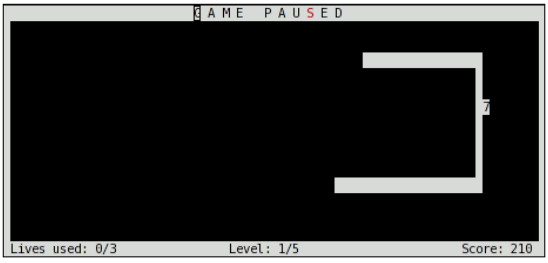
\includegraphics[scale=0.6]{./images/page203-1.png}
\end{center}

脚本的下载地址是 \url{http://www.vim.org/scripts/script.php?script_id=916}.

\subsection{魔方}
\label{subsec:rubik_s_cube}

% FIXME: 字母 o 本来有个双引号重音
1974 年, 匈牙利雕刻家兼建筑学教授 Erno Rubik 发明了一个由 27 个小方块组成的
魔方. 魔方的每一面分别涂上了一种不同的颜色. 如果试图旋转魔方, 那么魔方的颜色
就会变乱, 游戏的目标就是把一个弄乱了的魔方还原成最初的样子.

在 Rubik 发明了魔方的 30 年后, 2005 年, Olivier Vermersch 用 Vim 脚本开发了一
个魔方游戏. Vim 版的魔方同样会让玩家花费几个小时的时间, 把魔方复原.

\begin{center}
    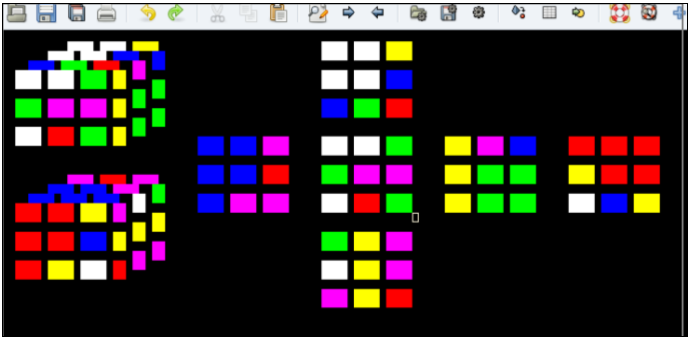
\includegraphics[scale=0.5]{./images/page203-2.png}
\end{center}

\marginpar{204}
游戏的使用方法与脚本的下载地址是
\url{http://www.vim.org/scripts/script.php?script_id=1271}

\subsection{井字棋}
\label{subsec:tic_tac_toe}
应该有很多小孩玩过井字棋 (Tic-Tac-Toe) 这个游戏.

1996 年, Kevin Earls 用一系列宏命令在 Vim 中实现了这个游戏, 游戏双方分别是人类
玩家和 Vim.

\begin{center}
    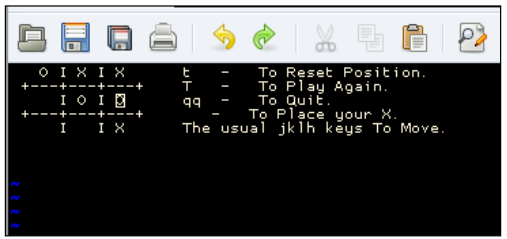
\includegraphics[scale=0.7]{./images/page204.png}
\end{center}

虽然 Vim 的智能不是很先进, 但是想要赢它还是比较困难的.

可以到 Earls 先生的个人主页上下载到游戏脚本, 脚本中包含了游戏的安装与使用方法,
下载地址是 \url{http://www.vanhemert.co.uk/vim/vimacros/ttt.vim}.

\subsection{扫雷}
\label{subsec:mines}

1995 年, 微软在新发布的操作系统 Windows 95 中, 预装了一个称为扫雷的小游戏.
这款游戏混合了数字谜语和一点运气. 玩家的目的是找出雷区中所有的地雷: 或者是
点击没有地雷的方块, 或者是在有地雷的方块上插一把旗子. 方块下的数字表示周围
8 个小方块下的地雷个数. 如果玩家计算出了地雷所在的位置, 就在地雷所在的方块上
插一把小旗子.
\marginpar{205}

2004 年, Charles E. Campbell 用 Vim 脚本重新实现了这个游戏, 游戏包含了多个
难度等级, 脚本的下载地址与使用方法在
\url{http://vim.sourceforge.net/scripts/script.php?script_id=551}.

\subsection{推箱子}
\label{subsec:sokoban}

我比较喜欢智力游戏, 也很喜欢推箱子. 游戏玩起来非常简单, 但是游戏本身却可以
非常得难. 游戏的内容是让一个小人把箱子推到指定的位置上. 听起来很简单是吗?
游戏的规则是一次只能推一个箱子, 而且只能推, 不能拉, 因此, 如果把箱子推到角落
中, 那就再也推不动它了, 这时候玩家就不得不重新开始游戏.

2002 年, Mike Sharpe 用 Vim 脚本实现了这个游戏, 游戏的关卡设计来自以前的
Linux 游戏 XSokoban. Mike Sharpe 尽量保持了用户接口的简单, 但游戏玩起来仍然
十分有趣.

\begin{warning}
    XSokoban 游戏可以到这个网址下载:
    \url{http://www.cs.cornell.edu/andru/xsokoban.html}.
\end{warning}

游戏脚本的下载地址是 \url{http://www.vim.org/scripts/script.php?script_id=211}.
\marginpar{206}

\subsection{俄罗斯方块}
\label{subsec:tetris}

最后要介绍的一款游戏是真正的经典 --- 俄罗斯方块, 游戏中会有不同大小与形状的
方块落下来, 玩家的目的是适当地对它们进行排列, 尽量使得每一行都是满的. 俄罗斯
方块是前苏联人 Alexey Pajitnov 在 1985 年发明的, 在这之后, 几乎每个平台都实现
了这个游戏, 而且产生了数以百计的变种.

\begin{center}
    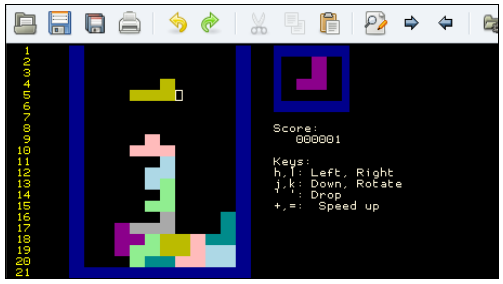
\includegraphics[scale=0.7]{./images/page206.png}
\end{center}

2002 年, Gergely Kontra 用 Vim 脚本实现了这个游戏, 游戏拥有不同的模式, 还可以
记录以前得过的最高分.

脚本的下载地址与使用方法在
\url{http://www.vim.org/scripts/script.php?script_id=172}.

\section{集成开发环境}
\label{sec:programmers_ide}

在书中我几次提到, Vim 可以帮助程序员完成很多事情, 从我个人来说, 几乎所有的
编程工作都是用 Vim 完成, 但有时候会听到其他程序员说: ``这么原始的编辑器你是怎
么用的?'', ``没有了集成开发环境, 你是怎么编程的?''. 其实, Vim 同样可以提供集
成开发环境.

首先来看一下集成开发环境应该提供哪些功能.
\marginpar{207}

一个典型的集成开发环境, 比如 Microsoft Windows Visual Studio\textregistered,
包括了下面这些组件:
\begin{itemize}
    \item 支持自动缩进, 语法高亮, 自动补全的编辑器
    \item 集成的编译器, 如果编译出错, 可以直接跳转到出错的地方
    \item 集成的调试器
    \item 文件浏览器
    \item 项目浏览器
    \item 标签浏览器, 通过它可以快速查看变量, 函数, 方法, 类
    \item 支持在文件间, 或定义间快速跳转
    \item 可能还集成了版本控制系统
\end{itemize}
那么, Vim 是否支持上面所说的全部特性呢? 我们逐条分析各个特性, 看一下 Vim
如何才能支持它们.

第一条是显而易见的, Vim 本身就是一个功能丰富的编辑器.

第二条是编译器的集成. Vim 通常用于编程工作, 因此它本身就支持编译器集成. 对
常见的编程语言来说, 和编译器集成相关的设置在 Vim 中本来就是设置好了的. 如果
不是, 可以用下面的方法查看如何设置它们:
\begin{vimcode}
:help compiler
\end{vimcode}
编译器集成通常会用到另一个功能: quickfix 列表. 当出现编译错误时, 程序员可以通
过这个列表跳转到出错的代码, 在各个错误之间前进或后退, 修正错误, 然后重新编译.

关于 quickfix 列表的更多信息, 可以查看:
\begin{vimcode}
:help quickfix
\end{vimcode}

下一条是集成的调试器. 和前一条不同的是, 对调试器的支持并不是 Vim 的标准特性.
但是有几个脚本可以帮助 Vim 集成调试器. 如果是 Linux, 可以用 VimDebug, 这个脚
本可以让 Vim 集成 gdb (C/C++ 调试器), jdb (Java 调试器), pdb (Python 调试器),
以及 Perl 调试器. 脚本的下载地址是
\url{http://www.vim.org/scripts/script.php?script_id=663}.
\marginpar{208}

另外一个功能更加丰富的调试器集成是 Clewn, 它集成了 gdb 调试器与 Vim, 支持调
试器的所有功能, 它甚至还支持远程调试. Clewn 的下载地址是
\url{http://clewn.sourceforge.net}.

再下一条是文件浏览器. Vim 本身就带有一个文件浏览器, 不过有一个脚本可以让文件
浏览器与集成开发环境更加搭配, 这个脚本是 VtreeExplorer. VtreeExplorer 不仅可
以浏览文件, 还可以把目录按照树状结构显示出来, 树的结点可以打开或折叠. 脚本的
下载地址是 \url{http://www.vim.org/scripts/script.php?script_id=184}.

接下来是集成开发环境的项目管理部分. 项目浏览器必须支持文件与项目的关联, 这样
的话, 当用户打开某个项目时, 项目内的所有文件就可以同时被打开. 如果用户用的是
Gvim, 就可以用 ProjMgr 脚本. ProjMgr 创建一个菜单项, 该菜单项包含了一张可用
项目列表, 除此之外, 它还可以创建新项目. 脚本的下载地址是
\url{http://vim.sourceforge.net/scripts/script.php?script_id=279}, 控制台版
本的下载地址是 \url{http://www.vim.org/scripts/script.php?script_id=69}.

对于标签浏览器, 有两种解决办法, 其中之一是执行标签名, 函数名, 和其他名字的
补全命令, 然后逐一浏览, 另一种办法是将所有可用的标签列在一个单独的窗口中, 为
了创建这样一个窗口, 我推荐 TagList 脚本. 只要是 Ctags 程序支持的编程语言,
TagList 都支持. 脚本会创建一个窗口, 这个窗口列出了所有的定义, 函数, 方法, 和
类, 不仅浏览方便, 还可以快速跳转到声明标签的地方. TagList 的下载地址是
\url{http://vim-taglist.sourceforge.net}.
\marginpar{209}

\begin{center}
    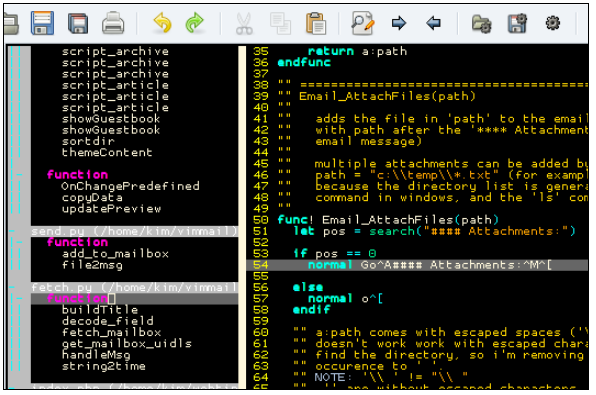
\includegraphics[scale=0.6]{./images/page209.png}
\end{center}
Vim 本身提供了两个命令: \texttt{gf} 与 \texttt{gd}, 分别用来跳转到标签所在
的文件与声明标签的地方, 通过这两个命令的帮助, 用户可以在文件中快速地移动.

最后要谈到的是版本控制系统, 比如 CVS, SVN 和 Perforce. 版本控制系统的集成同
样可以通过脚本来实现. 对于前面提到的三个版本控制系统, 我推荐以下几个脚本:
\begin{itemize}
    \item CVS 与 SVN 相关的脚本在
        \url{http://www.vim.org/scripts/script.php?script_id=90}
    \item Perforce 相关的脚本在
        \url{http://vim.sourceforge.net/scripts/script.php?script_id=240}
\end{itemize}

用来组装集成开发环境的各个组件都已经准备好了, 现在所要做的就是把它们都
集成起来. 可能有用户怕麻烦, 不想自己动手完成最后一步, 不用担心, 已经有其他人
帮你做好了. 比如 Vim JDE (Just a Development Environment), 它集成了上面提到
的所有脚本, 对 Java, C/C++ 程序员来说, 这是一个功能丰富的集成开发环境. Vim JDE
的下载地址是 \url{http://www.vim.org/scripts/script.php?script_id=1213}.
\marginpar{210}
另一种办法是在 Vim 社区中搜索集成脚本的方法, 然后按照方法所说的步骤执行,
比如 \url{http://vim.wikia.com/wiki/Using_vim_as_an_IDE_all_in_one}.

\section{邮件程序}
\label{sec:mail_program}

一直以来, Vim 就支持与多种不同的程序进行集成, 其中就包括一些邮件客户端, 比较
有名的客户端是 Mutt.

对于某些 Vim 用户来说, 与邮件客户端集成还远远不够, 于是他们决定用 Vim 脚本实现
一个完整的邮件客户端, 客户端的功能包括在 Vim 中直接收发和管理邮件.

\begin{warning}
    开源邮件客户端 Mutt 的下载地址是 \url{http://www.mutt.org/}.
\end{warning}

2004 年, Suresh Govindachar 为 Vim 开发了 The Mail Suite (TMS), 这个软件部分
用 Vim 脚本实现, 还有一部分用 Perl 脚本 (嵌入在 Vim 脚本代码) 实现. TMS 支持
邮件客户端的全部功能, 同时还可以用到 Vim 提供的所有特性.

TMS 的下载地址是 \url{http://www.vim.org/scripts/script.php?script_id=1052}.

2005 年, David Elentok 用一个 Vim 脚本和两个 Python 脚本实现了邮件客户端. 虽
然目前脚本还在开发阶段, 但邮件客户端的主要功能已经完成.

Elentok 的脚本的下载地址是
\url{http://www.vim.org/scripts/script.php?script_id=1346}.
\marginpar{211}

\section{聊天}
\label{sec:chat_with_vim}

在如今这个时代, 几乎找不到一台没有安装聊天程序的计算机, 但在过去可不是
这样. 回到 20 世纪 80 年代后期, 当时因特网上的聊天仅限于 BBS 的公告板. 到了
1988 年, 芬兰人 Jarkko Oikarinen 开发一个客户端/服务器模式的聊天程序 ---
Internet Relay Chat (IRC). 在接下来的十年, IRC 成为了一款非常流行的聊天程序,
越来越多的人开始加入到聊天网络中. IRC 的使用方法非常简单: 下载一个 IRC 客户
端, 用客户端连接到 IRC 服务器, 加入到一个你最喜欢的聊天频道, 接下来就可以和
别人畅所欲言了.

\begin{center}
	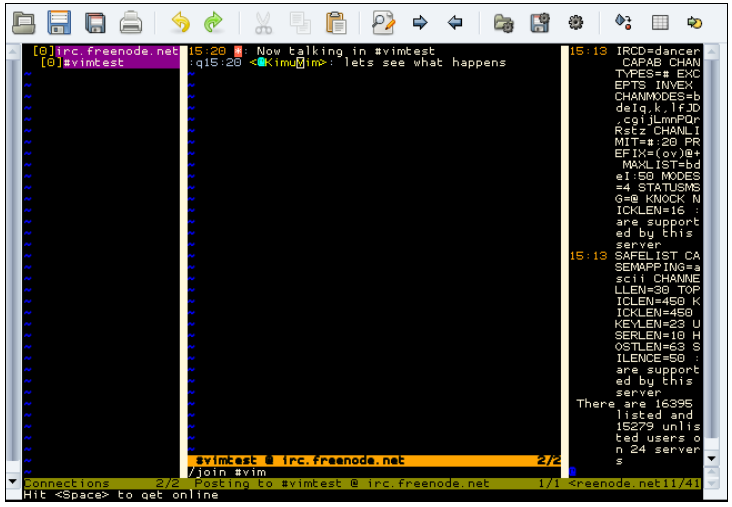
\includegraphics[scale=0.5]{./images/page211.png}
\end{center}

IRC 客户端版本众多, 2004 年, 日本人 Madoka Machitani 在 Vim 中实现了一个 IRC
客户端, 他把它叫作 VimIRC. VimIRC 功能丰富, 支持同时在多个网络的聊天频道中
聊天, 在客户端中还可以使用 Vim 命令, 比如 \texttt{I}, \texttt{/},
\texttt{?} 等.
\marginpar{212}

不过, 在 Vim 中聊天会有一个小问题. 为了让聊天保持在线, 客户端会执行一个循环
来不停地更新所有的东西. 如果用户移动到另一个和 IRC 客户端无关的缓冲区, 循环
就会停止, 用户的聊天网络最终就会断开. 解决这个问题的技巧是让客户端在自己的
Gvim 或 Vim 中启动, 这可以在命令行中完成:
\begin{vimcode}
gvim -i NONE -i .vimircrc -c VimIRC
\end{vimcode}
命令行中的 \texttt{.vimircrc} 是 VimIRC 配置文件的路径.

VimIRC 的下载地址是 \url{http://www.vim.org/scripts/script.php?script_id=931}.

\begin{warning}
    Vim 用户常去的 IRC 网络与频道分别是 \texttt{irc.freenode.net} 和
    \texttt{\#vim}.
\end{warning}

\section{Twitter 客户端}
\label{sec:using_vim_as_a_twitter_client}

最近几年社交网络变得越来越流行, Twitter (\url{http://www.twitter.com}) 是最流
行的社区平台之一, 它的主要功能是和朋友分享 ``状态更新''.

Po Shan Cheah 开发了一个 Vim 脚本, 使用这个脚本就可以在 Vim 中阅读朋友的状态
更新, 还可以直接发送自己的状态更新, 以及向 Twitter 朋友发送私人消息.

脚本的名字是 TwitVim, 下载地址是
\url{http://www.vim.org/scripts/script.php?script_id=2204}.

脚本的输出非常简单, 主要是列出用户所请求的朋友的最近一次状态更新, 它的示例输
出如下图所示:
\marginpar{213}
\begin{center}
    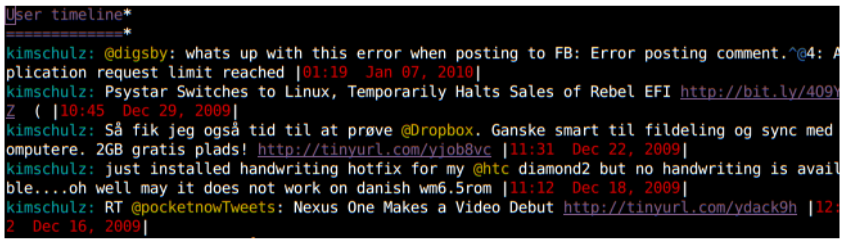
\includegraphics[scale=0.5]{./images/page213.png}
\end{center}

TwitVim 使用命令行程序 cURL (\url{http://curl.haxx.se/}) 从 Twitter 上抓取
信息, 因此在使用 TwitVim 之前, 要先下载安装 cURL.

\begin{warning}
    关于 Twitter 的更多信息, 请登录 \url{http://www.twitter.com}, 在那里可
    以免费注册一个账号.
\end{warning}

% End of appendix A

% vim: ts=4 sts=4 sw=4 tw=80
% FIXME
% 这个附录翻译得很不好, 有很多问题.
\chapter{Vim 配置管理}
\label{chap:vim_configuration_alternatives}
\marginpar{215}

第 \ref{chap:personalizing_vim} 章介绍了 Vim 的主要配置文件, 随着
阅读的深入, 我们不断地往 \texttt{vimrc} 中添加新的配置信息, 最终, 配置文件
可能会变得非常混乱, 难以管理.

本章将介绍一些组织 \texttt{vimrc} 的方法, 从小技巧一直到整个
配置系统.

最后, 将会介绍如何在多个不同的计算机中使用同一个 \texttt{vimrc} 文件,
方法是在网络中保存一份副本.

\section{保持 vimrc 整洁的技巧}
\label{sec:tips_for_keeping_your_vimrc_file_clean}

\texttt{vimrc} 是用户设置 Vim 的核心文件, 如果没有它, 就只能使用系统中原有
的设置, 因此用户要时刻保持 \texttt{vimrc} 的整洁, 并及时更新, 只有这样, 用
户才能时刻知道文件中包含了哪些内容. 有时候, 用户可能没办法在文件中找到自己
想要的内容, 笔者就曾经遇到过这种情况, 当时我的 \texttt{vimrc} 超过了 2000 行,
到那时才意识到整洁的必要性. 保持 \texttt{vimrc} 整洁并组织良好的技巧有:
\marginpar{216}
\begin{enumerate}
	\item 保持 Vim 处于非兼容模式

	这个技巧可能并不会让 \texttt{vimrc} 更整洁, 至少不能马上看出来, 然而
	它却非常重要. 让 Vim 处于非兼容模式下就可以打开许多特性, 而这些特性
	会被很多技巧和脚本使用到. 所以, 最好在 \texttt{vimrc} 的第一行总是写上
	\texttt{set nocompatible}.
	
	\item 使用注释

	有时候, 用户会在 Vim 中改变一些设置, 然后再把设置添加到 \texttt{vimrc},
	过一段时间后, 当用户想要清理 \texttt{vimrc} 时, 就会发现自己已经记不住
	某段脚本是干嘛用的, 以及当初为什么要添加它, 甚至连代码是从哪儿来的都已经记不清
	了. 为了防止这种情况发生, 那就给新加的东西写上注释. 笔者建议在注释中包含这
	些内容: 代码的作用 (描述), 从哪儿得到的 (来源), 代码的原作者. 有了注释的
	帮助, 用户就能够方便地查询到代码的来源, 以及决定是否需要删除它们. 注释
	用引号开始, 比如 \texttt{"This is a comment}.

	\item 数据分组

	脚本通常需要一些额外的设置, 或者是用户想要为脚本中的某些功能设置一些额外
	的按键绑定 (映射). 为了能更方便地看出设置的归属, 最好为数据分组. 分组的
	条件有很多种, 笔者推荐以下这些 (按照在文件中出现的顺序, 从上到下排列):
	\begin{itemize}
	  \item 通用的全局设置
	  \item 自己私有的按键映射
	  \item 特定于脚本的设置, 按脚本分组
	  \item 其他设置
	\end{itemize}

	\item 使用多个文件
	
	有时候, \texttt{vimrc} 可能会变得非常巨大, 无论怎么组织都显得非常混乱. 对
	于这种情况, 最好把它切分成多个文件. 为了切分 \texttt{vimrc}, 首先把需要分
	出的内容剪切到另一个文件中, 文件名最好能描述出文件的作用, 然后在
	\texttt{vimrc} 中原来的位置用 \texttt{source} 命令从新文件读取命令.
	比如, 把和按键映射相关的设置命令都移动到 \texttt{mappings.vim},
	然后在 \texttt{vimrc} 中添加 \texttt{source \$HOME/.vim/mappings.vim}.

\marginpar{217}
    \item 测试时使用其他文件

    从前, 当笔者想要测试某段新的 Vim 脚本代码或者宏时, 通常会把它们添加到
    \texttt{vimrc} 的末尾, 在测试结束后, 笔者往往会忘记把它们删除, 经过一段
    时间后, \texttt{vimrc} 就充满了我的测试代码. 为了避免重蹈覆辙, 读者
    应该把测试代码写在另一个文件中, 然后用 \texttt{source} 命令执行文件中的
    测试代码. 如果觉得不错, 就把代码移动到适当的地方, 否则, 只要把文件删掉即
    可.

	\item 为不同的操作系统使用不同的文件

	如果读者也像我一样, 在多个不同的系统中使用 Vim, 可能会发现有些配置不能
	适应全部的系统. 原因可能是因为有些设置是和操作系统相关的, 又或者是硬件
	配置不一样, 比如说有些系统的屏幕比较小, 而另一些则比较大. 如果出现这样
	的情况, 最好把系统相关的设置写在不同的文件中, 然后把通用的文件拷到所有
	的系统中, 再把系统相关的配置文件拷到各自的系统中.
\end{enumerate}

如果读者能够严格遵守这些技巧, 就很有希望把 \texttt{vimrc} 保持在一个非常整洁
的状态下, 这样的话, 无论想修改什么内容, 你都能快速地找到.

\section{vimrc 配置系统}
\label{sec:a_vimrc_setup_system}

使用 Vim 时, 为了永久地更改某项配置, 用户需要打开配置文件, 修改后再保存. 如果
只是在 Vim 中修改, 而没有写到配置文件中, 程序退出后, 所有的修改都会丢失.

假如有这样一个脚本, 它提供了一个设置菜单, 用户在其中所做的修改在程序退出后
仍然有效, 那将会怎样? Jos van RisWick 就开发出了这样的脚本.

通过使用他的脚本, 并按照他的语法来创建 \texttt{vimrc}, 用户不仅可以使新的配置
持久化, 还可以根据向导的指引, 一步步地对配置加以修改.

脚本的实现方式是, 把配置项周围的注释作为设置向导中所显示的信息的占位符.
笔者发现这个脚本非常聪明, 而且和我们通常用的不太一样, 所以我们在这里简单地介绍
一下如何使用它.
\marginpar{218}

脚本的下载地址是 \url{http://www.vim.org/scripts/script.php?script_id=1894},
下载的压缩包中包含了下面这些文件:
\begin{itemize}
  \item \texttt{setup.vim}: 主要的脚本
  \item \texttt{array.vim}: 包含了处理字符串数组的函数
  \item \texttt{arrayg.vim}: 包含了处理全局字符串数组的函数
  \item \texttt{strfun.vim}: 包含了字符串处理函数
  \item \texttt{tableaf.vim}: 用来在配置系统中显示 tab leaf
\end{itemize}

安装脚本的方法是把压缩包解压到 \texttt{VIMHOME} 目录下, 解压后, 文件就自动
放到了 \texttt{plugin/} 子目录中.

现在, 用户就可以准备好修改 \texttt{vimrc}, 但是在修改之前最好做个备份.

在我们开始往 \texttt{vimrc} 添加设置之前, 先来看一下配置系统的使用语法. 前
面已经说过, 技巧就是配置项周围的注释. 这些注释包含了很特殊的语法, 这样
脚本才能知道这些注释是干嘛用的, 语法的基本规则是
\texttt{"|ID|tabname|text|command|extra|val1|val2|val3|}.

其中每一项的意义如下表所示:
\begin{center}
  \begin{tabular}{lp{30em}}
  \hline
  项名 & 意义 \\
  \hline
   \texttt{"}	& 开始一个注释 \\
   \texttt{ID}	& 一个标识符, 脚本可以用它来区分不同的配置组. 当脚本启动时,
     用户要告诉脚本应该处理哪个配置组 \\
   \texttt{tabname} & 应用配置的 tab 的名字 (在脚本中称为 leaf) \\
   \texttt{text} & 和配置相关的文本信息 \\
   \texttt{command} & 配置项所要执行的实际命令, 比如 \texttt{set textwidth=},
     注意, 不需要填上具体的值 \\
	\hline
  \end{tabular}
\end{center}
\marginpar{219}
\begin{center}
	\begin{tabular}{lp{30em}}
	\hline
	  \texttt{extra} & 比如说, 如果命令是一个映射, 则变量部分就是被映射的
	  按键, 这时候用户还需要设置映射到的命令, 命令就是填在 \texttt{extra} 字
	  段中, 如果不需要它, 就留空 \\

	  \texttt{val1}-\texttt{val3} & 命令参数的默认值, 在配置系统中可以按
	  Tab 键来遍历这三个值. \\
	\hline
	\end{tabular}
\end{center}

再在来看一个例子:
\begin{vimcode}
"|SETTINGS|Layout|Set the text width|set tw=|50|70|90|
set tw=60
"|SETTINGS|Layout|Show a ruler?|let &ruler=||0|1|
let &ruler=1
\end{vimcode}
这个例子展示了设置 Vim 的两种典型方法 --- 用 \texttt{set} 与 \texttt{let} 来
设置一个选项. 在变量名左边加上 \texttt{\&} 是在告诉 Vim 等号右边的表达式要在
设置之前求值, 如果求值结果的类型和选项不一致, 还会自动转换类型. 注释下面是真
正的设置命令.

如果只是想在 tab 中添加一个注释, 只需要把命令替换成 \verb'%', 比如:
\begin{vimcode}
"|SETTINGS|Layout|Here you will find layout settings|%|
\end{vimcode}
用户还可以利用它来插入空行, 这些空行将作为间距来使用, 方法是用空格替换掉文本.

接下来讨论如何设置脚本.

设置脚本的地方在 \texttt{setup.vim}, 在脚本中搜索 \texttt{HERE2}, 找到该单词
出现的第二个地方, 你将会看到:
\begin{vimcode}
" Import settings from these files HERE2:
let setup_files=Arr("settings.vim", "mappings.vim", "scripts.vim")
let setup_group="SETTINGS"
\end{vimcode}
\marginpar{220}

\texttt{setup\_files} 是一个数组, 数组中的每一个元素都是一个文件名, 文件包含
了设置信息. 上面的例子用到了 \texttt{settings.vim},
\texttt{mappings.vim}, \texttt{scripts.vim} 这三个文件.

第二条命令告诉脚本当前设置使用哪一个配置组. 在示例中用的是
\texttt{SETTINGS}, 因此如果某个设置的注释以 \texttt{|SETTINGS|} 开始, 那么这
个设置就会被用到.

在开始使用配置向导之前, 在 \texttt{setup.vim} 中还有一项需要修改.

由于设置分散在多个文件中, 我们需要让 Vim 意识到这点, 因此 \texttt{vimrc} 要
包含 (在 Vim 中称为 source) 这些文件, 除此之外, 为了让修改生效, 还要让 Vim
重新加载 \texttt{vimrc}, 为了处理这种情况, 脚本提供了一个特殊的设置.

在 \texttt{setup.vim} 中搜索 \texttt{HERE1}, 找到单词出现的第二个地方, 用户
将会看到:
\begin{vimcode}
autocmd bufleave _setup source ~/.vimrc
\end{vimcode}
当用户离开配置向导时就会执行 \verb'source ~/.vimrc'. 如果需要的话, 用户
还可以添加其他外部配置文件.

现在讨论如何启动 Vim 配置向导, 并在向导中导航. 为了启动配置向导, 先切换到普通
模式, 然后按下 \texttt{s}, 启动后, 光标位于第一个 tab 的第一个设置上. 在向导
中有很多快捷键可以使用:
\begin{center}
  \begin{tabular}{ll}
    \hline
	快捷键  & 描述 \\
    \hline
    \texttt{r} 或 \texttt{R}  & 进入替换模式 \\
	\texttt{s} & 保存后退出 \\
	\texttt{q} & 不保存退出 \\
	\texttt{<space>} & 遍历所有的 tab leaf \\
	\texttt{j} & 跳转到当前 tab leaf 的下一个设置 \\
	\texttt{k} & 跳转到当前 tab leaf 的前一个设置 \\
	\texttt{<tab>} & 显示被选中的设置的可选值 \\
	\texttt{<cr>} & 接收当前行的修改 \\
	\texttt{<esc>} & 重新绘制当前的 tab leaf (普通模式) \\
	\texttt{<esc>} & 丢弃修改 (插入或替换模式) \\
	\hline
  \end{tabular}
\end{center}
\marginpar{221}

使用配置向导的准备工作就是这些. 下面的截图展示了向导的使用效果:
\begin{center}
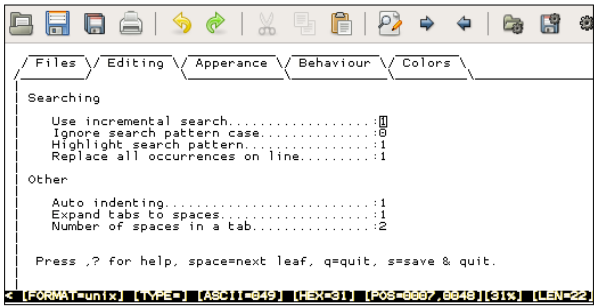
\includegraphics[scale=0.6]{./images/page221.png}
\end{center}

\section{在线存放 vimrc}
\label{sec:storing_vimrc_online}

假设用户要在多种不同的计算机中使用 Vim, 可能会因为每次都要重新设置 Vim, 或者
使用不同的设置而感到很恼火.

现在, 几乎每一台计算机都连接到了因特网上, 所以一个明显的解决办法是在线保存一
份 \texttt{vimrc}. 之前已经说过 Vim 可以编辑远程主机上的文件, 但是, 如果
要读取远程主机上的 \texttt{vimrc} 将会遇到一些问题. 通常情况下, 当 Vim 需要
读取网络上的文件时, 它会用到插件 \texttt{netrw}, 然而, 当 Vim 读取
\texttt{vimrc} 时, 这个插件还没有加载, 也就无法读取远程主机上的 \texttt{vimrc}.

解决办法是使用下面的函数:
\begin{vimcode}
function! GetNetVimrc(vimrc_url)
    source $VIMRUNTIME/plugin/netrwPlugin.vim
    Nread a:vimrc_url
    let tmpfile = tempname()
    save! tmpfile
    source tmpfile
    delete(tmpfile)
    enew
endfunction
\end{vimcode}
\marginpar{222}
读取 \texttt{vimrc} 的所有操作都在 \texttt{GetNetVimrc} 中完成. 函数的输入参数是
\texttt{vimrc} 的 URL 地址, 函数开始时先加载 \texttt{netrw} 插件, 加载后
Vim 就可以使用网络读写功能, 然后, 调用 \texttt{Nread} 从网络上读取
\texttt{vimrc} 到当前缓冲区, 再把文件的内容写到一个临时文件, 加载它, 最后再
把临时文件删掉, 并打开一个干净的缓冲区.

那么, 用户应该如何使用 \texttt{GetNetVimrc}?

首先把 \texttt{vimrc} 保存到网络上的某台主机, 如果用户想要在某个系统中使
用自己的在线 \texttt{vimrc}, 就把 \texttt{GetNetVimrc} 添加到系统本地的
\texttt{vimrc}.

调用函数的方式是:
\begin{vimcode}
:call GetNetVimrc("http://www.domain.com/myvimrc")
\end{vimcode}
还可以把上面这行代码添加到包含 \texttt{GetNetVimrc} 的 \texttt{vimrc} 文件中.

现在, 用户所有系统中的 Vim 都具有了相同的配置, 如果在线的 \texttt{vimrc} 有
了更新, 那么等下一次用户使用系统时, 这些更新也会反映在系统中.

记住, 用户还可以用 \texttt{Nread} 和 \texttt{Nwrite} 这两个函数来直接修改
在线 \texttt{vimrc}.

% end of appendix B

% vim: ts=4 sts=4 sw=4 tw=80
\chapter{索引}
\label{chap:index}

\marginpar{223}
索引中的页码指的是英文原版的页码, 与本书页边标注的页码一致.

\setlength\parindent{0pt}
\setlength\columnsep{1.5cm}
\setlength\columnseprule{0.4pt}

\begin{multicols}{2}

\hangindent=2pc \hangafter=1 \section*{符号}

\hangindent=2pc \hangafter=1 \texttt{:diffsplit} 112

\hangindent=2pc \hangafter=1 \texttt{:diffthis} 112

\hangindent=2pc \hangafter=1 \texttt{:pop} 82

\hangindent=2pc \hangafter=1 \texttt{:ptselect} 82

\hangindent=2pc \hangafter=1 \texttt{:tag} 82

\hangindent=2pc \hangafter=1 \texttt{:tnext} 82

\hangindent=2pc \hangafter=1 \texttt{:tprev} 82

\hangindent=2pc \hangafter=1 \texttt{:tselect} 82

\hangindent=2pc \hangafter=1 \texttt{:vert diffsplit} 112

\hangindent=2pc \hangafter=1 \texttt{<cWROD>} 61

\hangindent=2pc \hangafter=1 \texttt{<Leader>} 178

\hangindent=2pc \hangafter=1 \texttt{<Plug>} 178

\hangindent=2pc \hangafter=1 \texttt{<silent>} 31

\hangindent=2pc \hangafter=1 \texttt{<unique>} 178

\hangindent=2pc \hangafter=1 \section*{A}

\hangindent=2pc \hangafter=1 \texttt{AbbrAsk} 49

\hangindent=2pc \hangafter=1 \texttt{amenu} 33

\hangindent=2pc \hangafter=1 \texttt{argnum} 171

\hangindent=2pc \hangafter=1 Aspell 40

\hangindent=2pc \hangafter=1 autocompletion \par
\hangindent=2pc \hangafter=1\quad about (关于) 84 \par
\hangindent=2pc \hangafter=1\quad all-in-one completion (多合一补全) 89, 90 \par
\hangindent=2pc \hangafter=1\quad dictionary completion (字典补全) 85,86 \par
\hangindent=2pc \hangafter=1\quad known word completion (已知单词补全) 84,85 \par
\hangindent=2pc \hangafter=1\quad omnicompletion 86-88 \par

\hangindent=2pc \hangafter=1 \texttt{autoindent} 130

\hangindent=2pc \hangafter=1 \texttt{autoproto.vim} 84

\hangindent=2pc \hangafter=1 \section*{B}

\hangindent=2pc \hangafter=1 balloons 43

\hangindent=2pc \hangafter=1 Berkeley Par, external formatting tools (外部格式化工具) 137

\hangindent=2pc \hangafter=1 black hole register (黑洞寄存器) 102

\hangindent=2pc \hangafter=1 \texttt{buffers} 32

\hangindent=2pc \hangafter=1 \section*{C}

\hangindent=2pc \hangafter=1 \texttt{calcValue} 81

\hangindent=2pc \hangafter=1 charityware license (慈善授权) 15

\hangindent=2pc \hangafter=1 cindent \par
\hangindent=2pc \hangafter=1\quad about (关于) 131 \par
\hangindent=2pc \hangafter=1\quad setup options (配置选项) 131 \par

\hangindent=2pc \hangafter=1 code block formatting (代码块格式化) \par
\hangindent=2pc \hangafter=1\quad commands (命令) 133 \par

\hangindent=2pc \hangafter=1 code, formatting (代码格式化) \par
\hangindent=2pc \hangafter=1\quad about (关于) 129 \par
\hangindent=2pc \hangafter=1\quad \texttt{autoindent} 130 \par
\hangindent=2pc \hangafter=1\quad cindent 131 \par
\hangindent=2pc \hangafter=1\quad code-block, formatting (代码块格式化) 132-134 \par
\hangindent=2pc \hangafter=1\quad \texttt{indentexpr} 132 \par
\hangindent=2pc \hangafter=1\quad pasted code, auto formatting (自动格式化粘贴的代码) 135 \par
\hangindent=2pc \hangafter=1\quad settings (设置) 130 \par
\hangindent=2pc \hangafter=1\quad \texttt{smartindent} 130 \par

\hangindent=2pc \hangafter=1 color scheme (配色方案) 147

\hangindent=2pc \hangafter=1 color scheme, Vim (Vim 的配色方案) \par
\hangindent=2pc \hangafter=1\quad changing (修改) 21 \par

\hangindent=2pc \hangafter=1 configuration files (配置文件) \par
\hangindent=2pc \hangafter=1\quad \texttt{exrc} 19 \par
\hangindent=2pc \hangafter=1\quad \texttt{gvimrc} 19 \par
\hangindent=2pc \hangafter=1\quad types (配置文件的类型) 18 \par
\hangindent=2pc \hangafter=1\quad \texttt{vimrc} 18,19 \par

\hangindent=2pc \hangafter=1 context-aware navigation (基于上下文的导航) \par
\hangindent=2pc \hangafter=1\quad about (关于) 54 \par
\hangindent=2pc \hangafter=1\quad code file, moving around within (在代码文件内导航) 54, 55 \par
\hangindent=2pc \hangafter=1\quad code file, moving in (在代码文件内导航) 56-58 \par

\hangindent=2pc \hangafter=1 ctags command-line program (ctags 命令行程序) 80

\hangindent=2pc \hangafter=1 \texttt{ctags.vim} 83

\hangindent=2pc \hangafter=1 cURL 213

\hangindent=2pc \hangafter=1 \texttt{cursorline} 38

\hangindent=2pc \hangafter=1 \section*{D}

\hangindent=2pc \hangafter=1 debugger commands (调试器命令) \par
\hangindent=2pc \hangafter=1\quad about (关于) 187 \par
\hangindent=2pc \hangafter=1\quad \texttt{cont} 187 \par
\hangindent=2pc \hangafter=1\quad \texttt{finish} 187 \par
\hangindent=2pc \hangafter=1\quad \texttt{interrupt} 187 \par
\hangindent=2pc \hangafter=1\quad \texttt{next} 187 \par
\hangindent=2pc \hangafter=1\quad \texttt{quit} 187 \par
\hangindent=2pc \hangafter=1\quad \texttt{step} 187 \par

\hangindent=2pc \hangafter=1 debugging (调试) \par
\hangindent=2pc \hangafter=1\quad Vim scripts (Vim 脚本) 186-188 \par

\hangindent=2pc \hangafter=1 drop registers (投递寄存器) 102

\hangindent=2pc \hangafter=1 \section*{E}

\hangindent=2pc \hangafter=1 editor area, Vim (Vim 的编辑器区域) \par
\hangindent=2pc \hangafter=1\quad abbreviations, using (使用缩写) 46-48 \par
\hangindent=2pc \hangafter=1\quad key bindings, modifying (修改按键绑定) 49, 51 \par
\hangindent=2pc \hangafter=1\quad line numbers, adding (添加行号) 39 \par
\hangindent=2pc \hangafter=1\quad personalizing (个性化) 37 \par
\hangindent=2pc \hangafter=1\quad spell check (拼写检查) 40-42 \par
\hangindent=2pc \hangafter=1\quad tooltip, adding (工具提示) 43-46 \par
\hangindent=2pc \hangafter=1\quad editor area, Vim visual cursor, adding (添加可视化光标) 37, 38 \par

\hangindent=2pc \hangafter=1 Elvis \par
\hangindent=2pc \hangafter=1\quad about (关于) 10 \par
\hangindent=2pc \hangafter=1\quad features (特性) 10 \par

\hangindent=2pc \hangafter=1 Emacs editor (Emacs 编辑器) 13

\hangindent=2pc \hangafter=1 expression register (表达式寄存器) 103

\hangindent=2pc \hangafter=1 \texttt{exrc} 19

\hangindent=2pc \hangafter=1 external formatting tools (外部格式化工具) \par
\hangindent=2pc \hangafter=1\quad about (关于) 136 \par
\hangindent=2pc \hangafter=1\quad Berkeley Par 137 \par
\hangindent=2pc \hangafter=1\quad Indent 136 \par
\hangindent=2pc \hangafter=1\quad Tidy 138 \par
\hangindent=2pc \hangafter=1\quad using (使用方法) 136 \par

\hangindent=2pc \hangafter=1 external interpreter (外部解释器) \par
\hangindent=2pc \hangafter=1\quad using in Vim scripting (在 Vim 脚本中使用) 194 \par

\hangindent=2pc \hangafter=1 \section*{F}

\hangindent=2pc \hangafter=1 file explorer (文件浏览器) 208

\hangindent=2pc \hangafter=1 file navigation (文件导航) \par
\hangindent=2pc \hangafter=1\quad about (关于) 54 \par
\hangindent=2pc \hangafter=1\quad context-aware navigation (基于上下文的导航) 54 \par
\hangindent=2pc \hangafter=1\quad long line, navigating (长行导航) 59 \par

\hangindent=2pc \hangafter=1 File-Type plugins group (文件类型插件组) 148

\hangindent=2pc \hangafter=1 fold (折叠) \par
\hangindent=2pc \hangafter=1\quad about (关于) 107 \par
\hangindent=2pc \hangafter=1\quad \texttt{diff}, using to track changes (使用 \texttt{diff} 跟踪差异) 114 \par
\hangindent=2pc \hangafter=1\quad simple text file outlining (简单的文本文件提纲) 110, 111 \par
\hangindent=2pc \hangafter=1\quad types (类型) 107 \par
\hangindent=2pc \hangafter=1\quad using (使用方法) 107-109 \par
\hangindent=2pc \hangafter=1\quad \texttt{vimdiff}, using to track changes (使用 \texttt{vimdiff} 跟踪差异) 111 \par

\hangindent=2pc \hangafter=1 \texttt{foldclose()} 45

\hangindent=2pc \hangafter=1 fonts, Vim (Vim 字体) \par
\hangindent=2pc \hangafter=1\quad changing (修改) 20 \par

\hangindent=2pc \hangafter=1 \texttt{for} loop (\texttt{for} 循环) 164, 165

\hangindent=2pc \hangafter=1 \texttt{formatexpr} 123

\hangindent=2pc \hangafter=1 formatting, Vim (Vim 格式化) \par
\hangindent=2pc \hangafter=1\quad code, formatting (代码格式化) 129 \par
\hangindent=2pc \hangafter=1\quad external formatting tools, using (使用外部格式化工具) 136 \par
\hangindent=2pc \hangafter=1\quad text, formatting (文本格式化) 121 \par

\hangindent=2pc \hangafter=1 functions (函数) \par
\hangindent=2pc \hangafter=1\quad creating (创建) 168-170 \par
\hangindent=2pc \hangafter=1\quad variable argument list (可变参数列表) 170-172 \par

\hangindent=2pc \hangafter=1 \section*{G}

\hangindent=2pc \hangafter=1 Game of Life (生命游戏) 202

\hangindent=2pc \hangafter=1 \texttt{get} 163

\hangindent=2pc \hangafter=1 Global plugins group (全局插件组) 148

\hangindent=2pc \hangafter=1 \texttt{guitablabel} 属性 36

\hangindent=2pc \hangafter=1 \texttt{gvimrc} 19

\hangindent=2pc \hangafter=1 \section*{H}

\hangindent=2pc \hangafter=1 hacker (黑客) 15

\hangindent=2pc \hangafter=1 hacking 15

\hangindent=2pc \hangafter=1 \texttt{hasmapto()} 178

\hangindent=2pc \hangafter=1 \texttt{helpgrep} 67

\hangindent=2pc \hangafter=1 hidden markers (隐藏标记) \par
\hangindent=2pc \hangafter=1\quad about (关于) 71 \par
\hangindent=2pc \hangafter=1\quad marks, using (使用标记) 71 \par

\hangindent=2pc \hangafter=1 \section*{I}

\hangindent=2pc \hangafter=1 IDE (集成开发环境) 208

\hangindent=2pc \hangafter=1 \texttt{indentexpr} 132

\hangindent=2pc \hangafter=1 Indent, external formatting tools (外部格式化工具) 136

\hangindent=2pc \hangafter=1 integrated compiler (集成的编译器) 207

\hangindent=2pc \hangafter=1 integrated debugger (集成的调试器) 207

\hangindent=2pc \hangafter=1 interpreter (解释器) 15
\hangindent=2pc \hangafter=1 Ispell 40

\hangindent=2pc \hangafter=1 \section*{J}

\hangindent=2pc \hangafter=1 \texttt{join} 163

\hangindent=2pc \hangafter=1 \section*{K}

\hangindent=2pc \hangafter=1 key bindings, editor area (按键绑定) \par
\hangindent=2pc \hangafter=1\quad modifying (修改) 49, 51 \par

\hangindent=2pc \hangafter=1 \texttt{keys()} 165

\hangindent=2pc \hangafter=1 \texttt{keyvar} 165

\hangindent=2pc \hangafter=1 \section*{L}

\hangindent=2pc \hangafter=1 line numbers, editor area (行号) \par
\hangindent=2pc \hangafter=1\quad adding (添加) 39 \par

\hangindent=2pc \hangafter=1 \texttt{loaded\_myscript} 176

\hangindent=2pc \hangafter=1 \texttt{LoadTemplate} 77

\hangindent=2pc \hangafter=1 \texttt{lookupfile.vim} 83

\hangindent=2pc \hangafter=1 loops (循环) \par
\hangindent=2pc \hangafter=1\quad about (关于) 164 \par
\hangindent=2pc \hangafter=1\quad \texttt{for} loop (\texttt{for} 循环) 164 \par
\hangindent=2pc \hangafter=1\quad types (类型) 164 \par
\hangindent=2pc \hangafter=1\quad \texttt{while} loop (\texttt{while} 循环) 164 \par

\hangindent=2pc \hangafter=1 \section*{M}

\hangindent=2pc \hangafter=1 marcro recording (宏录制) \par
\hangindent=2pc \hangafter=1\quad about (关于) 90 \par
\hangindent=2pc \hangafter=1\quad using (使用方法) 90-92 \par

\hangindent=2pc \hangafter=1 \texttt{map} 30, 163

\hangindent=2pc \hangafter=1 \texttt{marks} (书签) 71

\hangindent=2pc \hangafter=1 matching features, Vim (Vim 的匹配特性) 22

\hangindent=2pc \hangafter=1 \texttt{menu} 30

\hangindent=2pc \hangafter=1 MicroEmacs code (MicroEmacs 的代码) 13

\hangindent=2pc \hangafter=1 Mines (扫雷) 204

\hangindent=2pc \hangafter=1 MS Visual Studio\textregistered 207

\hangindent=2pc \hangafter=1 Mutt 210

\hangindent=2pc \hangafter=1 \texttt{mydict} dictionary (字典 \texttt{mydict}) 165

\hangindent=2pc \hangafter=1 \texttt{MyIndenter()} 132

\hangindent=2pc \hangafter=1 \section*{N}

\hangindent=2pc \hangafter=1 named registers (命名寄存器) 101

\hangindent=2pc \hangafter=1 navigation, in multiple buffers (在多个缓冲区中导航) 61

\hangindent=2pc \hangafter=1 navigation, in Vim help (在 Vim 帮助系统中导航) 60

\hangindent=2pc \hangafter=1 Nibbles (贪吃蛇) 202

\hangindent=2pc \hangafter=1 numbered registers (编号的寄存器) 100

\hangindent=2pc \hangafter=1 nvi \par
\hangindent=2pc \hangafter=1\quad about (关于) 10 \par
\hangindent=2pc \hangafter=1\quad features (特性) 11 \par

\hangindent=2pc \hangafter=1 \section*{O}

\hangindent=2pc \hangafter=1 omnicompletion 86-88

\hangindent=2pc \hangafter=1 \section*{P}

\hangindent=2pc \hangafter=1 Perl 195

\hangindent=2pc \hangafter=1 personal hightlighting, Vim (Vim 的修改化高亮) \par
\hangindent=2pc \hangafter=1\quad about (关于) 22, 23 \par
\hangindent=2pc \hangafter=1\quad color character, marking (彩色字符标记) 24 \par
\hangindent=2pc \hangafter=1\quad errors, preventing (抑制错误) 26 \par
\hangindent=2pc \hangafter=1\quad tabs not used for indentation, marking (标记不是用作缩进的制表符) 25 \par

\hangindent=2pc \hangafter=1 \texttt{PrintSum} 169

\hangindent=2pc \hangafter=1 project browser (项目浏览器) 208

\hangindent=2pc \hangafter=1 Python 196

\hangindent=2pc \hangafter=1 \section*{R}

\hangindent=2pc \hangafter=1 \texttt{range()} 164

\hangindent=2pc \hangafter=1 read-only registers (只读寄存器) 101

\hangindent=2pc \hangafter=1 registers (寄存器) \par
\hangindent=2pc \hangafter=1\quad about (关于) 98 \par
\hangindent=2pc \hangafter=1\quad drop registers (投递寄存器) 102 \par
\hangindent=2pc \hangafter=1\quad expression registers (表达式寄存器) 103 \par
\hangindent=2pc \hangafter=1\quad named registers (命名寄存器) 101 \par
\hangindent=2pc \hangafter=1\quad numbered registers (带编号的寄存器) 100 \par
\hangindent=2pc \hangafter=1\quad read-only registers (只读寄存器) 101 \par
\hangindent=2pc \hangafter=1\quad search pattern register (搜索模式寄存器) 102 \par
\hangindent=2pc \hangafter=1\quad selection register (选择寄存器) 102 \par
\hangindent=2pc \hangafter=1\quad small delete register (小删除寄存器) 100 \par
\hangindent=2pc \hangafter=1\quad unnamed register (匿名寄存器) 100 \par
\hangindent=2pc \hangafter=1\quad using (使用方法) 99 \par

\hangindent=2pc \hangafter=1 remote files (远程文件) \par
\hangindent=2pc \hangafter=1\quad editing (编辑) 117, 118 \par
\hangindent=2pc \hangafter=1\quad working in (处理远程文件) 115-117 \par

\hangindent=2pc \hangafter=1 Rubik's cube (魔方) 203

\hangindent=2pc \hangafter=1 Ruby 198

\hangindent=2pc \hangafter=1 \section*{S}

\hangindent=2pc \hangafter=1 script (脚本) 15

\hangindent=2pc \hangafter=1 script development (脚本开发) \par
\hangindent=2pc \hangafter=1\quad about (关于) 150, 151 \par
\hangindent=2pc \hangafter=1\quad script writing basic (脚本开发基础) 151 \par

\hangindent=2pc \hangafter=1 scripting tips, Vim (Vim 脚本开发技巧) \par
\hangindent=2pc \hangafter=1\quad Gvim, using (使用 Gvim) 182 \par
\hangindent=2pc \hangafter=1\quad longer lines, printing (打印长行) 185 \par
\hangindent=2pc \hangafter=1\quad multiple operating system, working with (处理多个操作系统) 183 \par
\hangindent=2pc \hangafter=1\quad versions, of Vim (Vim 的版本) 183 \par

\hangindent=2pc \hangafter=1 script writing basics (脚本开发基础) \par
\hangindent=2pc \hangafter=1\quad about (关于) 151 \par
\hangindent=2pc \hangafter=1\quad conditions (条件) 157, 158 \par
\hangindent=2pc \hangafter=1\quad dictionaries, working with (处理字典) 159-163 \par
\hangindent=2pc \hangafter=1\quad functions, creating (创建函数) 168 \par
\hangindent=2pc \hangafter=1\quad lists, working with (处理线性表) 159-163 \par
\hangindent=2pc \hangafter=1\quad loops (循环) 164 \par
\hangindent=2pc \hangafter=1\quad types (类型) 152 \par
\hangindent=2pc \hangafter=1\quad variables (变量) 153-157 \par

\hangindent=2pc \hangafter=1 \texttt{scrollbind} 113

\hangindent=2pc \hangafter=1 search pattern register (搜索模式寄存器) 102

\hangindent=2pc \hangafter=1 search, Vim (Vim 搜索) \par
\hangindent=2pc \hangafter=1\quad examples (例子) 64, 65 \par
\hangindent=2pc \hangafter=1\quad help system, searching (在帮助系统中搜索) 67 \par
\hangindent=2pc \hangafter=1\quad searching, in current file (在当前文件中搜索) 64 \par
\hangindent=2pc \hangafter=1\quad searching, in multiple files (在多个文件中搜索) 65, 66 \par

\hangindent=2pc \hangafter=1 selection registers (选择寄存器) 102

\hangindent=2pc \hangafter=1 \texttt{sessionoptions} \par
\hangindent=2pc \hangafter=1\quad \texttt{blank} 96 \par
\hangindent=2pc \hangafter=1\quad \texttt{buffers} 96 \par
\hangindent=2pc \hangafter=1\quad \texttt{curdir} 96 \par
\hangindent=2pc \hangafter=1\quad \texttt{folds} 96 \par
\hangindent=2pc \hangafter=1\quad \texttt{globals} 96 \par
\hangindent=2pc \hangafter=1\quad \texttt{help} 96 \par
\hangindent=2pc \hangafter=1\quad \texttt{localoptions} 96 \par
\hangindent=2pc \hangafter=1\quad \texttt{options} 96 \par
\hangindent=2pc \hangafter=1\quad \texttt{resize} 96 \par
\hangindent=2pc \hangafter=1\quad \texttt{sesdir} 96 \par
\hangindent=2pc \hangafter=1\quad \texttt{slash} 96 \par
\hangindent=2pc \hangafter=1\quad \texttt{tabpages} 96 \par
\hangindent=2pc \hangafter=1\quad \texttt{unix} 96 \par
\hangindent=2pc \hangafter=1\quad \texttt{winpos} 96 \par
\hangindent=2pc \hangafter=1\quad \texttt{winsize} 96 \par

\hangindent=2pc \hangafter=1 sessions (会话) \par
\hangindent=2pc \hangafter=1\quad \texttt{sessionoptions} 96 \par
\hangindent=2pc \hangafter=1\quad simple session usage (会话的简单用法) 93-95 \par
\hangindent=2pc \hangafter=1\quad using (使用方法) 93 \par
\hangindent=2pc \hangafter=1\quad using, as project manager (项目管理程序) 97, 98 \par

\hangindent=2pc \hangafter=1 setup options, cindent (cindent 的设置选项) \par
\hangindent=2pc \hangafter=1\quad \texttt{cinkeys} 131 \par
\hangindent=2pc \hangafter=1\quad \texttt{cinoptions} 131 \par
\hangindent=2pc \hangafter=1\quad \texttt{cinwords} 131 \par

\hangindent=2pc \hangafter=1 \texttt{ShortTabLine()} 35

\hangindent=2pc \hangafter=1 \texttt{sign} 68

\hangindent=2pc \hangafter=1 Single Unix Specification (SUS, 单一 Unix 规范) 9

\hangindent=2pc \hangafter=1 small delete register (小删除寄存器) 100

\hangindent=2pc \hangafter=1 \texttt{smartindent} 130

\hangindent=2pc \hangafter=1 snipMate plugin (snipMate 插件) 79

\hangindent=2pc \hangafter=1 snipMate system (snipMate 系统) 79

\hangindent=2pc \hangafter=1 Sokoban (推箱子) 205

\hangindent=2pc \hangafter=1 \texttt{sort()} 165

\hangindent=2pc \hangafter=1 \texttt{spelllang} 40

\hangindent=2pc \hangafter=1 \texttt{spellsuggest()} 45

\hangindent=2pc \hangafter=1 \texttt{split} 163

\hangindent=2pc \hangafter=1 status line, Vim (Vim 的状态行) 26, 28

\hangindent=2pc \hangafter=1 STEVIE 9

\hangindent=2pc \hangafter=1 \texttt{suffixadd} 62

\hangindent=2pc \hangafter=1 \texttt{sum} 170

\hangindent=2pc \hangafter=1 syntax coloring (语法高亮) 142, 143, 147

\hangindent=2pc \hangafter=1 syntax-color scheme (语法高亮主题) 141

\hangindent=2pc \hangafter=1 syntax regions (语法区) 143-146

\hangindent=2pc \hangafter=1 \section*{T}

\hangindent=2pc \hangafter=1 tabs, Vim (Vim 的标签页) \par
\hangindent=2pc \hangafter=1\quad modifying (修改) 33-37 \par

\hangindent=2pc \hangafter=1 tag browser (Tag 浏览器) 208

\hangindent=2pc \hangafter=1 tag list generators (Tag list 生成程序) \par
\hangindent=2pc \hangafter=1\quad about (关于) 80 \par
\hangindent=2pc \hangafter=1\quad Ctags 80 \par
\hangindent=2pc \hangafter=1\quad Hdrtags 80 \par
\hangindent=2pc \hangafter=1\quad Jtags 80 \par
\hangindent=2pc \hangafter=1\quad Ptags 80 \par
\hangindent=2pc \hangafter=1\quad Vtags 80 \par

\hangindent=2pc \hangafter=1 tag lists \par
\hangindent=2pc \hangafter=1\quad about (关于) 80 \par
\hangindent=2pc \hangafter=1\quad taglist navigation (taglist 导航) 83 \par
\hangindent=2pc \hangafter=1\quad uses 83 \par
\hangindent=2pc \hangafter=1\quad using (使用方法) 80-82 \par

\hangindent=2pc \hangafter=1 \texttt{taglist.vim} 83

\hangindent=2pc \hangafter=1 templates (模版) \par
\hangindent=2pc \hangafter=1\quad abbreviations, using (使用缩写) 76, 77 \par
\hangindent=2pc \hangafter=1\quad about (关于) 74 \par
\hangindent=2pc \hangafter=1\quad snippets, with snipMate script (通过 snipMate 使用代码片断) 78, 79 \par
\hangindent=2pc \hangafter=1\quad template files, using (使用模版文件) 74, 75 \par

\hangindent=2pc \hangafter=1 Tetris (俄罗斯方块) 206

\hangindent=2pc \hangafter=1 text, formatting (文本格式化) \par
\hangindent=2pc \hangafter=1\quad about (关于) 121 \par
\hangindent=2pc \hangafter=1\quad headlines, marking (标题行标记) 125, 126 \par
\hangindent=2pc \hangafter=1\quad lists, creating (创建线性表) 127-129 \par
\hangindent=2pc \hangafter=1\quad text, aligning (文本对齐) 124 \par
\hangindent=2pc \hangafter=1\quad text, putting into paragraph (文本分段) 122, 123 \par

\hangindent=2pc \hangafter=1 The Mail Suite (TMS, 邮件套装) 210

\hangindent=2pc \hangafter=1 Tic-Tac-Toe (井字棋) 204

\hangindent=2pc \hangafter=1 Tidy, external formatting tools (外部格式化工具 Tidy) 138

\hangindent=2pc \hangafter=1 TwitVim 212

\hangindent=2pc \hangafter=1 \section*{U}

\hangindent=2pc \hangafter=1 undo branching (撤消分支) \par
\hangindent=2pc \hangafter=1\quad about (关于) 98 \par
\hangindent=2pc \hangafter=1\quad using (使用方法) 103-106 \par

\hangindent=2pc \hangafter=1 unnamed register (匿名寄存器) 100

\hangindent=2pc \hangafter=1 \section*{V}

\hangindent=2pc \hangafter=1 variables (变量) \par
\hangindent=2pc \hangafter=1\quad about (关于) 153 \par
\hangindent=2pc \hangafter=1\quad dictionary (字典) 153 \par
\hangindent=2pc \hangafter=1\quad \texttt{funcref} 153 \par
\hangindent=2pc \hangafter=1\quad list (线性表) 153 \par
\hangindent=2pc \hangafter=1\quad number (数值) 153 \par
\hangindent=2pc \hangafter=1\quad string (字符串) 153 \par

\hangindent=2pc \hangafter=1 \texttt{v:folddashes} 109

\hangindent=2pc \hangafter=1 \texttt{v:foldend} 109

\hangindent=2pc \hangafter=1 \texttt{v:foldstart} 109

\hangindent=2pc \hangafter=1 vi 9

\hangindent=2pc \hangafter=1 vi compatibility (vi 兼容性) 14, 15

\hangindent=2pc \hangafter=1 Vile \par
\hangindent=2pc \hangafter=1\quad about (关于) 13 \par
\hangindent=2pc \hangafter=1\quad features (特性) 13 \par

\hangindent=2pc \hangafter=1 Vim \par
\hangindent=2pc \hangafter=1\quad about (关于) 7, 11 \par
\hangindent=2pc \hangafter=1\quad advanced formatting (高级格式化) 121 \par
\hangindent=2pc \hangafter=1\quad autocompletion (自动补全) 84 \par
\hangindent=2pc \hangafter=1\quad charityware license (慈善授权) 15 \par
\hangindent=2pc \hangafter=1\quad color scheme, changing (修改配色方案) 21 \par
\hangindent=2pc \hangafter=1\quad command line buffer (命令行寄存器) 26 \par
\hangindent=2pc \hangafter=1\quad configuration files (配置文件) 18 \par
\hangindent=2pc \hangafter=1\quad download link (下载链接) 8 \par
\hangindent=2pc \hangafter=1\quad editor area, personalizing (个性化的编辑区) 37 \par
\hangindent=2pc \hangafter=1\quad extensibility (可扩展性) 141 \par
\hangindent=2pc \hangafter=1\quad features (特性) 12 \par
\hangindent=2pc \hangafter=1\quad fonts, changing (修改字体) 20 \par
\hangindent=2pc \hangafter=1\quad hidden markers (隐藏标记) 71 \par
\hangindent=2pc \hangafter=1\quad mail program (邮件程序) 210 \par
\hangindent=2pc \hangafter=1\quad marks, adding (添加标记) 68 \par
\hangindent=2pc \hangafter=1\quad matching (匹配) 22 \par
\hangindent=2pc \hangafter=1\quad menu, adding (添加菜单) 29-32 \par
\hangindent=2pc \hangafter=1\quad menu, toggling (切换菜单) 28, 29 \par
\hangindent=2pc \hangafter=1\quad personal highlighting (个性化高亮) 22, 23 \par
\hangindent=2pc \hangafter=1\quad personalizing (个性化) 17 \par
\hangindent=2pc \hangafter=1\quad scripting tips (脚本开发技巧) 182 \par
\hangindent=2pc \hangafter=1\quad script structure (脚本结构) 175 \par
\hangindent=2pc \hangafter=1\quad search (搜索) 63 \par
\hangindent=2pc \hangafter=1\quad status line (状态行) 26 \par
\hangindent=2pc \hangafter=1\quad syntax-color schemes (语法配色方案) 141 \par
\hangindent=2pc \hangafter=1\quad tabs, modifying (修改标签页) 33-37 \par
\hangindent=2pc \hangafter=1\quad toolbar icons, adding (添加工具栏图标) 32, 33 \par
\hangindent=2pc \hangafter=1\quad toolbar, toggling (切换工具栏) 28, 29 \par
\hangindent=2pc \hangafter=1\quad using, as Twitter client (Twitter 客户端) 212 \par
\hangindent=2pc \hangafter=1\quad visible markers (可视化的标记) 68-70 \par

\hangindent=2pc \hangafter=1 Vimballs \par
\hangindent=2pc \hangafter=1\quad creating (创建) 190 \par

\hangindent=2pc \hangafter=1 \texttt{vimdiff} \par
\hangindent=2pc \hangafter=1\quad about (关于) 112 \par
\hangindent=2pc \hangafter=1\quad navigation (导航) 113 \par
\hangindent=2pc \hangafter=1\quad using, to track changes (跟踪差异) 111 \par

\hangindent=2pc \hangafter=1 \texttt{vimdiff} session (\texttt{vimdiff} 会话) 112

\hangindent=2pc \hangafter=1 Vim documentation (Vim 文档) 191, 193

\hangindent=2pc \hangafter=1 Vim games (Vim 游戏) \par
\hangindent=2pc \hangafter=1\quad about (关于) 201 \par
\hangindent=2pc \hangafter=1\quad Game of Life (生命游戏) 202 \par
\hangindent=2pc \hangafter=1\quad Mines (扫雷) 204 \par
\hangindent=2pc \hangafter=1\quad Nibbles (贪吃蛇) 202 \par
\hangindent=2pc \hangafter=1\quad Rubik's cube (魔方) 203 \par
\hangindent=2pc \hangafter=1\quad Sokoban (推箱子) 205 \par
\hangindent=2pc \hangafter=1\quad Tetris (俄罗斯方块) 206 \par
\hangindent=2pc \hangafter=1\quad Tic-Tac-Toe (井字棋) 204 \par

\hangindent=2pc \hangafter=1 VimIRC 211, 212

\hangindent=2pc \hangafter=1 \texttt{vimrc} \par
\hangindent=2pc \hangafter=1\quad about (关于) 18, 19 \par
\hangindent=2pc \hangafter=1\quad cleaning, tips (清理技巧) 215 \par
\hangindent=2pc \hangafter=1\quad online storing (在线存储) 221 \par

\hangindent=2pc \hangafter=1 \texttt{vimrc} file, cleaning tips (\texttt{vimrc} 清理技巧) \par
\hangindent=2pc \hangafter=1\quad comments, using (使用注释) 216 \par
\hangindent=2pc \hangafter=1\quad data, grouping (数据分组) 216 \par
\hangindent=2pc \hangafter=1\quad multiple files, using (使用多个文件) 216 \par
\hangindent=2pc \hangafter=1\quad Vim, using in noncompatible mode (在非兼容模式中使用 Vim) 216 \par

\hangindent=2pc \hangafter=1 \texttt{vimrc} setup system (\texttt{vimrc} 设置系统) \par

\hangindent=2pc \hangafter=1 Vim script (Vim 脚本) \par
\hangindent=2pc \hangafter=1\quad debugging (调试) 186-188 \par
\hangindent=2pc \hangafter=1\quad distributing (发布) 189 \par
\hangindent=2pc \hangafter=1\quad external interpreters, using (外部解释器) 194 \par
\hangindent=2pc \hangafter=1\quad installing (安装) 148, 149 \par
\hangindent=2pc \hangafter=1\quad scripting tips (脚本开发技巧) 182 \par
\hangindent=2pc \hangafter=1\quad structure (结构) 175 \par
\hangindent=2pc \hangafter=1\quad types (类型) 148 \par
\hangindent=2pc \hangafter=1\quad uninstalling (卸载) 150 \par
\hangindent=2pc \hangafter=1\quad using (使用方法) 147 \par

\hangindent=2pc \hangafter=1 Vim scripting, in Perl (使用 Perl 开发 Vim 脚本) 195, 196

\hangindent=2pc \hangafter=1 Vim scripting, in Python (使用 Python 开发 Vim 脚本) 196, 197

\hangindent=2pc \hangafter=1 Vim scripting, in Ruby (使用 Ruby 开发脚本) 198, 199

\hangindent=2pc \hangafter=1 Vimi script structure (Vim 脚本结构) \par
\hangindent=2pc \hangafter=1\quad about (关于) 175 \par
\hangindent=2pc \hangafter=1\quad functions (函数) 178, 179 \par
\hangindent=2pc \hangafter=1\quad key mappings (按键映射) 178, 179 \par
\hangindent=2pc \hangafter=1\quad script configuration (脚本配置) 177 \par
\hangindent=2pc \hangafter=1\quad script header (脚本头部信息) 176 \par
\hangindent=2pc \hangafter=1\quad script-loaded check (脚本加载检查) 176 \par

\hangindent=2pc \hangafter=1 visible markers (可视化标记) \par
\hangindent=2pc \hangafter=1\quad about (关于) 68-70 \par
\hangindent=2pc \hangafter=1\quad \texttt{sign}, using (使用 \texttt{sign}) 68-70 \par

\hangindent=2pc \hangafter=1 visual cursor, editor area (可视化光标) \par
\hangindent=2pc \hangafter=1\quad adding (添加) 37 \par

\hangindent=2pc \hangafter=1 \section*{W}

\hangindent=2pc \hangafter=1 \texttt{while} loop (\texttt{while} 循环) 166, 167

\hangindent=2pc \hangafter=1 \section*{X}

\hangindent=2pc \hangafter=1 xvile 13

\hangindent=2pc \hangafter=1 \end{multicols}


\backmatter

\end{document}
